%\documentclass[a4paper,10pt]{article}
\documentclass[10pt]{scrartcl}
%\usepackage[IL2]{fontenc}
\usepackage[utf8x]{inputenc}
\usepackage[czech]{babel}
\usepackage{listings}  
\usepackage{amsfonts,amsmath,amssymb,graphicx,color}
%\usepackage[total={17cm,27cm}, top=2cm, left=2cm, includefoot]{geometry}
%\usepackage{fancyhdr}
\usepackage{fkssugar}
\usepackage{hyperref}
\usepackage{mhchem}

%\usepackage{caption}

%  Umožňuje rozdělovat obsah na více sloupců
\usepackage{multicol}
\usepackage{booktabs}
\usepackage{pgffor}


% FJFI Types of popi
\renewcommand{\popi}[2]{$\frac{#1}{[\jd{#2}]}$}

\renewcommand{\figurename}{Obr.}
\addto\captionsczech{\renewcommand{\figurename}{Obr.}}
\addto\captionsczech{\renewcommand{\tablename}{Tab.}}
\def\mean#1{\left< #1 \right>}


\newcommand{\MakeFJFIHead}{
\setlength{\parindent}{0cm}
\begin{multicols}{2}
\textsf{\textbf{\FJFISubject \hspace{6.25cm} \FJFIInstitute}\\
\textbf{\large{\FJFITitle}}}

\begin{tabular}{rlrl}
	 \textsf{Jméno:} & \textbf{\textsf\FJFIAuthor}    &      \textsf{Kolega:} & \textsf{\FJFICoauthor} \\[1.5pt]
	  \textsf{Kruh:} & \textbf{\textsf\FJFIGroup}     & \textsf{Číslo skup.:} & \textsf{\FJFICircle}   \\[1.5pt]
	\textsf{Měřeno:} & \textbf{\textsf{\FJFILabdate}} &  \textsf{Zpracování}: & \textsf{\FJFIWorktime}
\end{tabular}

\begin{flushright}


\includegraphics[scale=0.2]{../img/fjfi.pdf}
%\hspace{0.4cm}
%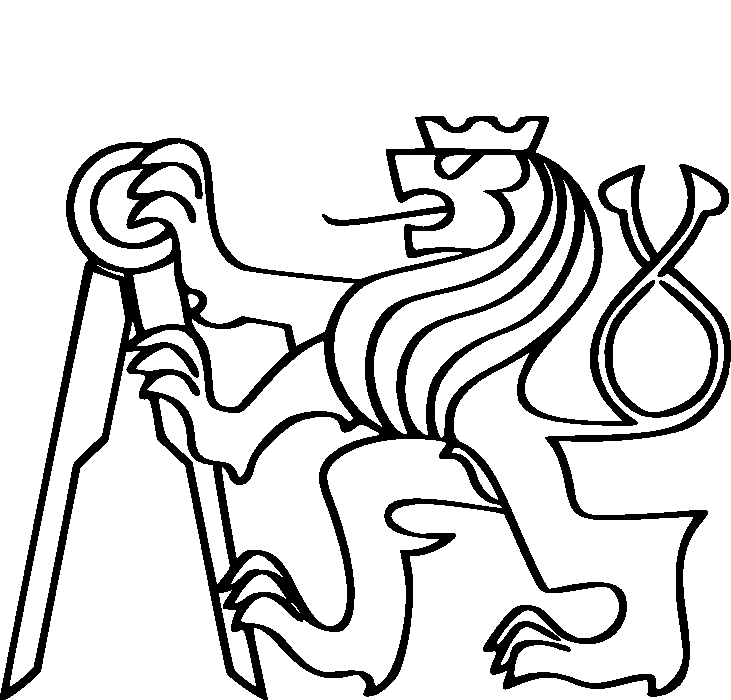
\includegraphics[scale=0.2]{../img/cvut.pdf}


\textsf{Klasifikace:} \hspace{3.2cm} 

\end{flushright}
\end{multicols}

\hrule
}




%  Nastaví autora, název, datum, skupinu měření apod. 
\newcommand{\Institute}{FJFI~ČVUT~v~Praze}
%\newcommand{\Subject}{Základy fyzikálních měření}
\newcommand{\Subject}{Fyzikální praktikum II}  %odkomentujte dle potřeby

%  Máte-li více spoluměřících než jednoho, vložte jen jejich příjmení
\newcommand{\Author}{Michal Červeňák}
\newcommand{\Coauthor}{Ondrej Glac} 
\newcommand{\Group}{Útorok} %den, kdy chodíte na praktika, nikoli obor
\newcommand{\Circle}{1} %číslo skupiny v rámci praktika, nikoli kruh

%  Tato část bude v každém protokolu jiná, nezapomeňte upravit!
\newcommand{\Title}{}
\newcommand{\Labdate}{28.2.2017} %datum měření, nikoli datum odevzdání
\newcommand{\Worktime}{\infy h} %jak dlouho vám trvalo vypracování protokolu


\begin{document}

\MakeFJFIHead{}

\section{Pracovní úkol}
\begin{enumerate}
\item DU: Odvo ďte vzorec (1) pro Brewsterův úhel úplné polarizace. Vycházejte z Obr. 1 a ze zákona lomu světla na rozhraní dvou optických prostředí. Spočtěte
Brewsterův úhel pro rozhraní vzduch - skleněné zrcadlo. Při měření Brewsterova
úhlu se doporučuje mít připravenou tabulku v Excelu pro výpočet stupně polarizace.
\item Při polarizaci bílého světla odrazem na černé skleněné desce proměřte závislost stupně polarizace
na sklonu desky a určete optimální hodnotu Brewsterova úhlu. Výsledky zaneste do grafu
a porovnejte s vypočtenou hodnotou z domácího úkolu.
\item Cernou otočnou desku nahraďte polarizačním filtrem a proměřte závislost intenzity polarizo-vaného světla na úhlu otočení analyzátoru (Malusův zákon). Výsledek srovnejte s teoretickou
předpovědí, znázorněte graficky a výsledek diskutujte.
\item Na optické lavici prozkoumejte vliv čtyř celofánových dvojlomných filtrů, způsobujících interferenci.
Vyzkoušejte vliv otáčení analyzátoru vůči polarizátoru a vliv otáčení dvojlomného filtru
mezi zkříženými i rovnoběžnými polarizátory v bílém světle. Pozorováním zjistěte, které vlnové
délky (barvy) se interferencí zvýrazní. Výsledky pozorování popište.
\item Pomocí dvou polarizačních filtrů, fotočlánku a barevných filtrů změřte měrnou otáčivost
křemene s tloušťkou 1 mm pro 4 vlnové délky světla. Jakou závislost pozorujete mezi vlnovou
délkou světla a měrnou otáčivostí? Naměřené hodnoty porovnejte s tabulkovými. Jak se změní
výsledek když použijete křemenný vzorek s větší tloušťkou? Diskutujte naměřené výsledky.
\end{enumerate}



\section{Teória}
Cievkou s $n_1$ závitami navinutej na toroide o polomere $r$, prechádza prúd $I_M$ 
Potom pre túto cievku môžeme intenzitu magnetického poľa $H$ vyjadriť ako
\eq{
H=\frac{n_1 I_M}{2\pi r}\,. \lbl{R_1}
}

Pre zmenu magnetickej indukcie $B$ v závislosti na výchylke balistického galvanometru $s$ platí vzťah 
\eq{
\Delta B = \frac{B K_b \lambda s_1^{*}}{n_2 S} \,, \lbl{R_2}
}
pričom $K_b$ je balistická konštanta, $R$ je odpor na odporovej dekáde, $s_1^{*}$ je výchylka galvanometra a $n_2$ počet meracích závitov. 

pre balistickú konštantu platí 
\eq{
R K_b \lambda = \frac{2L_{12} I_i}{s_1}\,,
}
kde $L_{12}$ je normálová cievka so známou indukčnosťou, a $s_1$ je výchylka pri zmene prúdu o $I_i$

%%%%%%%%%%%%%%%%%%%%%%%%%%%%%%%%%%%%%%%=
\subsubsection{Spracovanie chýb merania}

Označme $\mean{t}$ aritmetický priemer nameraných hodnôt $t_i$, a $\Delta t$ hodnotu $\mean{t}-t$, pričom 
\eq{
\mean{t} = \frac{1}{n}\sum_{i=1}^n t_i \,, \lbl{SCH_1}
}  
a chybu aritmetického priemeru 
\eq{
  \sigma_0=\sqrt{\frac{\sum_{i=1}^n \(t_i - \mean{t}\)^2}{n\(n-1\)}}\,, \lbl{SCH_2}
}
pričom $n$ je počet meraní.






\section{Pomôcky}

Scintilační detektor, zdroj vysokého napětí NL2410, čítač impulsů NL2301, jednokanálový
analyzátor, multikanálový analyzátor PHYWE, osciloskop, PC, zdroje gama
záření, olověné destičky, program MEASURE.

\section{Postup merania}
Scintilátor bol pripojený k zdroju napätia a pripojený k osciloskopu. 
Na detektor bol položený meraný žiarič.
Bola vyhotovená fotografia obrazu na osciloskope.


Následne bol osciloskop prepojený a scintilátor bol pripojený k mnohokanálovému analyzátoru a jeho výstup k počítaču.
Postupne boli namerané všetky žiariče, pozadie, a známe žiariče, u ktorých bolo medzi detektor a žiarič vložených niekoľko olovených doštičiek.


\section{Výsledky merania}
\subsection{Šošovka \uv{+200}}

Pre spojku \uv{+200} boli hodnoty zaznamenané v Tab. \ref{T_1}.
Pomocou programu \LaTeX\footnote{balíček metapost, ktorý je súčasťou distribúcie texlive-full.}
boli graficky určené polohy ohniskových vzdialeností $f_i$ pre jednotlivé merania 
\eq[m]{
\vect f_1 &= "[20.30\pm0.05,16.88\pm0.05] cm" \,,\\
\vect f_2 &= "[-,-]"\,,\\
\vect f_3 &= "[18.13\pm0.05,18.55\pm0.05] cm" \,,\\
\vect f_4 &="[17.70\pm0.05,18.92\pm0.05] cm" \,,
}
pričom pre druhé meranie sa nepodarilo určiť priesečník.
Zo zvyšných troch bodov bolo vypočítané ťažisko $\vect f="[18.71\pm0.9,18.12\pm0.8] cm" $ a pomocou vzťahu \ref{SCH_1} určená smerodajná odchylka, z $\vect f$ bola určená $f_g ="184.1\pm11.1 mm"$.

Z tabuľky pomocou vzťahu \ref{SCH_1} a \ref{SCH_2} sa určili mohutnosť šošovky $f\_B="181.76\pm4.87 mm"$.

\begin{table}[h]
\begin{center}
\begin{tabular}{ |  c | c | c | c | c | c | }
\hline
\popi{s_1}{cm}& \popi{s_2}{cm} & \popi{s_z}{cm}& \popi{s_o}{cm} & \popi{f\_B}{mm} & \popi{f_g}{mm} \\
\hline
$"50.20\pm0.05"$ & $"71.50\pm0.05"$ & $"100.0\pm0.1"$ & $"20.0\pm0.1"$ & $"185.82\pm0.1"$ & $"185.8\pm18.0"$\\ 
$"62.70\pm0.05"$ & $"65.50\pm0.05"$ & $"100.0\pm0.1"$ & $"30.0\pm0.1"$ & $"174.68\pm0.1"$ & $"-"$\\ 
$"35.50\pm0.05"$ & $"74.20\pm0.05"$ & $"100.0\pm0.1"$ & $"10.0\pm0.1"$ & $"183.34\pm0.1"$ & $"183.4\pm2.1"$\\ 
$"42.10\pm0.05"$ & $"73.70\pm0.05"$ & $"100.0\pm0.1"$ & $"15.0\pm0.1"$ & $"183.13\pm0.1"$ & $"183.1\pm5.1"$\\ 
\hline
\end{tabular}
\caption{Namerané hodnoty pre spojku \uv{+200}, pričom $s_1$ a $s_2$ sú polohy šošovky na dráhe, $s_o$ je poloha tienidla na dráhe, $s_z$ je poloha o zdroja (predmetu) na dráhe, $f\_B$ je vypočítané ohnisko Besselovou metodóu podľa vzťahu \ref{R_1} a $f_g$ je ohnisko učené grafickou metódou.} \label{T_1}
\end{center}
\end{table}

\subsection{Mikroskopický objektív}

Namerané hodnoty sú zaznamenané v tabuľke Tab. \ref{T_2} a z hodnôt $f\_B$ vypočítané pomocou vzťahu \ref{SCH_1} a \ref{SCH_2} vypočítaná ohnisková vzdialenosť $f = "92.15\pm2.63 mm"$.
Ďalej bola určená poloha ohniskových rovín, 
zdroj svetla bol umiestnený na optickej lavici $s_z="\(93.0\pm0.5\) cm"$, 
objektív $s_o="\(87.8\pm0.1\) cm"$, teda $x="\(52\pm6\) mm"$.
\begin{table}[h]
\begin{center}
\begin{tabular}{ |  c | c | c | c | c |  }
\hline
\popi{s_1}{cm}& \popi{s_2}{cm} & \popi{s_z}{cm}& \popi{s_o}{cm} & \popi{f\_B}{mm} \\
\hline
$"47.50\pm0.05"$ & $"88.70\pm0.05"$ & $"93.0\pm0.5"$ & $"30.0\pm0.1"$ & $"90.1\pm0.6"$ \\ 
$"37.30\pm0.05"$ & $"88.60\pm0.05"$ & $"93.0\pm0.5"$ & $"20.0\pm0.1"$ & $"92.4\pm0.6"$ \\ 
$"27.40\pm0.05"$ & $"88.80\pm0.05"$ & $"93.0\pm0.5"$ & $"10.0\pm0.1"$ & $"93.9\pm0.6"$ \\ 

\hline
\end{tabular}
\caption{Namerané hodnoty pre mikroskopický objektív, pričom $s_1$ a $s_2$ sú polohy šošovky na dráhe, $s_o$ je poloha tienidla na dráhe, $s_z$ je poloha o zdroja (predmetu) na dráhe, $f\_B$ je vypočítané ohnisko Besselovou metódou podľa vzťahu \ref{R_1}.} \label{T_2}
\end{center}
\end{table}

\subsection{Ramsdenový objektív}
Namerané hodnoty sú zaznamenané v tabuľke Tab. \ref{T_3} a z hodnôt $f\_B$ vypočítané pomocou vzťahu \ref{SCH_1} a \ref{SCH_2} vypočítaná ohnisková vzdialenosť $f = "93.27\pm0.73 mm"$.

Ďalej bola určená poloha ohniskových rovín, zdroj svetla bol umiestnený na optickej lavici $s_z="\(93.0\pm0.5\) cm"$, objektív $s_o="\(81.7\pm0.1\) cm"$, teda $x="\(113\pm6\) mm"$.

\begin{table}[h]
\begin{center}
\begin{tabular}{ |  c | c | c | c | c |  }
\hline
\popi{s_1}{cm}& \popi{s_2}{cm} & \popi{s_z}{cm}& \popi{s_o}{cm} & \popi{f\_B}{mm} \\
\hline
$"74.40\pm0.05"$ & $"92.80\pm0.05"$ & $"93.0\pm0.5"$ & $"50.0\pm0.1"$ & $"87.8\pm0.6"$ \\ 
$"64.30\pm0.05"$ & $"92.90\pm0.05"$ & $"93.0\pm0.5"$ & $"40.0\pm0.1"$ & $"93.9\pm0.6"$ \\ 
$"54.30\pm0.05"$ & $"93.00\pm0.05"$ & $"93.0\pm0.5"$ & $"30.0\pm0.1"$ & $"98.0\pm0.6"$ \\ 

\hline
\end{tabular}
\caption{Namerané hodnoty pre Ramsdenový objektív, pričom $s_1$ a $s_2$ sú polohy šošovky na dráhe, $s_o$ je poloha tienidla na dráhe, $s_z$ je poloha o zdroja (predmetu) na dráhe, $f\_B$ je vypočítané ohnisko Besselovou metódou podľa vzťahu \ref{R_1} } \label{T_3}
\end{center}
\end{table}


\subsection{Lupa}
Zväčšenie lupy bolo priamou metódou, pričom referenčná stupnica bola umiestnená do vzdialenosti $l="\(25\pm1\) cm"$ a presnosť určenia počtu dielikov bol $"1 dielik" = "10 \%"$ určené na $Z_l=10\pm1$. 


\subsection{Ďalekohľad}
Zväčšenie ďalekohľadu sme určili na základne porovnania zorných uhlov , pričom sme videli jeden dielik v ďalekohľade ako 20 dielikov \uv{vzoru} teda zväčšenie je $Z = 20\pm1$.

\begin{figure}
\includegraphics{data/graph_a.eps}
\caption{Grafické riešenie čočkovej rovnice pre spojku, kde malé body sú priesečniky $\vect f_i , i\in \{1,3,4\}$, šedý veľký krúžok je zistené ohnisko, a čierny je predpokladané ohnisko, čiarkovanou čiarou je druhé meranie, ktoré sa nepretína.}  \label{G_1}
\end{figure}



\section{Diskusia}

V prvej časti sme videli spektrum na osciloskope kde nám hrúbka (svetlosť) čiary vyjadruje intenzitu daného kanálu.
Ekvivalentom hrúbky čiary je jej jasnosť toho sme využili a za pomoci analýzy fotky sme vyniesli spektrum.
Fotka nieje nijak moc kvalitná a fotoaparát nieje kalibrovaný, či už súdkovitosť obrazu, jasnosť alebo citlivosť v rôznych častiach farbeného spektra.
Zároveň nemáme ani zkalibrovanú osu $x$.

Pri pokuse napojiť a skúmať spektrum cez jedno-kanálový analyzátor sa nám nepodarilo toto spektrum namerať.

Pri zapojení do multikanálového analyzátoru sme namerali jednotlivé spektrá. 

Všetky žiariče boli umiestnené v nepriehľadných krabičkćh. Pri pokladaní a výmene vzorkov sa teda mohli vzorky v krabičke otočiť alebo inak zmeniť polohu, a teda ich intenzita mohla byť iná pri rôznych meraniach.

Detekcia píkov, hlavne píkov ktoré sú blízko pri sebe je veľmi nepresná a hlavne pri \ce{Ba} sa jednotlivé píky kryli. Teda pri fitovaní bola zvolená postupná metóda kde bol určený prvý pík a ten odčítaný od spektra a z tohoto nového spektra bol určený ďalší pík. Táto metóda má svoje nevýhody, však na tieto dáta je sa podľa môjho názoru zdala najprijateľnejšia. 

Jednotlivé takto nájdené piky boli použité pri kalibrácii. 

Pomocou kalibračnej krivky bolo preškálované spektrum neznámeho vzorku. Nakoniec bol pomocou tabuľky \cite{C_3} ako \ce{^{134}Cs}. 
Pri určovaní sa hľadal v danej tabuľke žiarič s dlhším ako niekoľkodňovým polčasom rozpadu, 
ktorý má pik najväčší pík okolo energie $E="767.68 keV"$. 
Cézium \ce{^{134}Cs} má píky v $E="795.864\pm0.004 keV"$ a $E="801.953\pm0.004 keV"$, 
ktoré sa javia pri našom rozlíšení ako jeden pík. 
Ďalší charakteristický črt vidíme v okolí nameranej energie $E="544.78\pm4.412 keV"$, 
kde podľa tabuľkových údajov vyskytuje skupina píkov o energiách 
$E ="563.246\pm0.005 keV"$, $E ="569.331\pm0.003 keV"$ a $E ="604.721\pm0.002 keV"$, 
kde je síce naše spektrum posunuté ale to je spôsobené už horeuvedenými dôvodmi.

Následne bolo použitých 5 doštičiek z olova ako tienenie a namerané spektrum. Tu sa sa pri spracovaní ukázalo, že by bolo vhodné pre potreby spracovania namerať aj tienené pozadie. Doštičky položené na detektroe nám nechcene odlifrovali aj časť pozadia a teda pri odčítaní pozadia nám vychádzali záporné hodnoty. Z tohoto dôvodu som sa pri výpočte tienenia rozhodol neodčítať pozadie. 

Fitovanie pomeru útlmu, $I_0/I$, sme robili len v oblasti do $"500 keV"$ resp. do $"700 keV"$, kde ešte neprevládal šum. 

Comptonovo kontinum a Comptonovu hranu som určil z grafu tohoto dôvodu bola chyba stanovená na $"\pm20 keV"$. 

Pík úplného pohltenia ani pík spätného rozptylu sa mi nepodarilo v spektre určiť.

Zároveň sme zistili, že vzorka \ce{^{241}Am} nežiarí alebo má pre nás nemerateľnú aktivitu. 

\section{Záver}
Boli namerané spektrá jednotlivých žiaričov a určené píky. Podľa nich určená kalibračná krivka \ref{R_kal}.

Následne bol určený koeficient útlmu olova \ref{R_u}. 

A určený neznámy žiarič ako \ce{^{134}Cs}.


\begin{thebibliography}{2}
\bibitem{C_1}
gama spektroskopia [cit. 18.04.2017]Dostupné po prihlásení z Kurz: Fyzikální praktikum II:\url{https://praktikum.fjfi.cvut.cz/pluginfile.php/420/mod_resource/content/15/Gamma%20170217.pdf}
\bibitem{C_2}
Online Spectrum Catalogs for Ge and Si(Li) [cit. 18.04.2017] Idaho National Laboratory :\url{http://www4vip.inl.gov/gammaray/catalogs/ge/catalog_ge.shtml}
\bibitem{C_3}
Gamma Energy (KeV) [cit. 18.04.2017] Idaho National Laboratory :\url{https://www.cpp.edu/~pbsiegel/bio431/genergies.html}


\section{Prílohy}
\newpage

\begin{figure}
\includegraphics{data/graph_1.jpg}
\caption{Spektálne čiary pozorované osciloskopom}\label{G_cs}
\end{figure}

\begin{figure}
% GNUPLOT: LaTeX picture
\setlength{\unitlength}{0.240900pt}
\ifx\plotpoint\undefined\newsavebox{\plotpoint}\fi
\sbox{\plotpoint}{\rule[-0.200pt]{0.400pt}{0.400pt}}%
\begin{picture}(1500,900)(0,0)
\sbox{\plotpoint}{\rule[-0.200pt]{0.400pt}{0.400pt}}%
\put(171.0,131.0){\rule[-0.200pt]{4.818pt}{0.400pt}}
\put(151,131){\makebox(0,0)[r]{ 120}}
\put(1419.0,131.0){\rule[-0.200pt]{4.818pt}{0.400pt}}
\put(171.0,235.0){\rule[-0.200pt]{4.818pt}{0.400pt}}
\put(151,235){\makebox(0,0)[r]{ 140}}
\put(1419.0,235.0){\rule[-0.200pt]{4.818pt}{0.400pt}}
\put(171.0,339.0){\rule[-0.200pt]{4.818pt}{0.400pt}}
\put(151,339){\makebox(0,0)[r]{ 160}}
\put(1419.0,339.0){\rule[-0.200pt]{4.818pt}{0.400pt}}
\put(171.0,443.0){\rule[-0.200pt]{4.818pt}{0.400pt}}
\put(151,443){\makebox(0,0)[r]{ 180}}
\put(1419.0,443.0){\rule[-0.200pt]{4.818pt}{0.400pt}}
\put(171.0,547.0){\rule[-0.200pt]{4.818pt}{0.400pt}}
\put(151,547){\makebox(0,0)[r]{ 200}}
\put(1419.0,547.0){\rule[-0.200pt]{4.818pt}{0.400pt}}
\put(171.0,651.0){\rule[-0.200pt]{4.818pt}{0.400pt}}
\put(151,651){\makebox(0,0)[r]{ 220}}
\put(1419.0,651.0){\rule[-0.200pt]{4.818pt}{0.400pt}}
\put(171.0,755.0){\rule[-0.200pt]{4.818pt}{0.400pt}}
\put(151,755){\makebox(0,0)[r]{ 240}}
\put(1419.0,755.0){\rule[-0.200pt]{4.818pt}{0.400pt}}
\put(171.0,859.0){\rule[-0.200pt]{4.818pt}{0.400pt}}
\put(151,859){\makebox(0,0)[r]{ 260}}
\put(1419.0,859.0){\rule[-0.200pt]{4.818pt}{0.400pt}}
\put(169.0,131.0){\rule[-0.200pt]{0.400pt}{4.818pt}}
\put(169,90){\makebox(0,0){ 0}}
\put(169.0,839.0){\rule[-0.200pt]{0.400pt}{4.818pt}}
\put(367.0,131.0){\rule[-0.200pt]{0.400pt}{4.818pt}}
\put(367,90){\makebox(0,0){ 100}}
\put(367.0,839.0){\rule[-0.200pt]{0.400pt}{4.818pt}}
\put(565.0,131.0){\rule[-0.200pt]{0.400pt}{4.818pt}}
\put(565,90){\makebox(0,0){ 200}}
\put(565.0,839.0){\rule[-0.200pt]{0.400pt}{4.818pt}}
\put(762.0,131.0){\rule[-0.200pt]{0.400pt}{4.818pt}}
\put(762,90){\makebox(0,0){ 300}}
\put(762.0,839.0){\rule[-0.200pt]{0.400pt}{4.818pt}}
\put(960.0,131.0){\rule[-0.200pt]{0.400pt}{4.818pt}}
\put(960,90){\makebox(0,0){ 400}}
\put(960.0,839.0){\rule[-0.200pt]{0.400pt}{4.818pt}}
\put(1158.0,131.0){\rule[-0.200pt]{0.400pt}{4.818pt}}
\put(1158,90){\makebox(0,0){ 500}}
\put(1158.0,839.0){\rule[-0.200pt]{0.400pt}{4.818pt}}
\put(1356.0,131.0){\rule[-0.200pt]{0.400pt}{4.818pt}}
\put(1356,90){\makebox(0,0){ 600}}
\put(1356.0,839.0){\rule[-0.200pt]{0.400pt}{4.818pt}}
\put(171.0,131.0){\rule[-0.200pt]{0.400pt}{175.375pt}}
\put(171.0,131.0){\rule[-0.200pt]{305.461pt}{0.400pt}}
\put(1439.0,131.0){\rule[-0.200pt]{0.400pt}{175.375pt}}
\put(171.0,859.0){\rule[-0.200pt]{305.461pt}{0.400pt}}
\put(30,495){\makebox(0,0){\popi{\text{brightness}}{1/2.55 \%}}}
\put(805,29){\makebox(0,0){\popi{x}{px}}}
\put(1279,819){\makebox(0,0)[r]{spekturm}}
\put(1439,833){\makebox(0,0){$+$}}
\put(1437,251){\makebox(0,0){$+$}}
\put(1435,214){\makebox(0,0){$+$}}
\put(1433,225){\makebox(0,0){$+$}}
\put(1431,230){\makebox(0,0){$+$}}
\put(1429,251){\makebox(0,0){$+$}}
\put(1427,271){\makebox(0,0){$+$}}
\put(1425,256){\makebox(0,0){$+$}}
\put(1423,251){\makebox(0,0){$+$}}
\put(1421,277){\makebox(0,0){$+$}}
\put(1419,282){\makebox(0,0){$+$}}
\put(1417,271){\makebox(0,0){$+$}}
\put(1415,245){\makebox(0,0){$+$}}
\put(1413,209){\makebox(0,0){$+$}}
\put(1411,204){\makebox(0,0){$+$}}
\put(1409,235){\makebox(0,0){$+$}}
\put(1407,256){\makebox(0,0){$+$}}
\put(1405,261){\makebox(0,0){$+$}}
\put(1403,303){\makebox(0,0){$+$}}
\put(1401,287){\makebox(0,0){$+$}}
\put(1399,261){\makebox(0,0){$+$}}
\put(1397,245){\makebox(0,0){$+$}}
\put(1395,245){\makebox(0,0){$+$}}
\put(1394,266){\makebox(0,0){$+$}}
\put(1392,292){\makebox(0,0){$+$}}
\put(1390,313){\makebox(0,0){$+$}}
\put(1388,303){\makebox(0,0){$+$}}
\put(1386,303){\makebox(0,0){$+$}}
\put(1384,308){\makebox(0,0){$+$}}
\put(1382,313){\makebox(0,0){$+$}}
\put(1380,323){\makebox(0,0){$+$}}
\put(1378,329){\makebox(0,0){$+$}}
\put(1376,334){\makebox(0,0){$+$}}
\put(1374,334){\makebox(0,0){$+$}}
\put(1372,349){\makebox(0,0){$+$}}
\put(1370,339){\makebox(0,0){$+$}}
\put(1368,349){\makebox(0,0){$+$}}
\put(1366,365){\makebox(0,0){$+$}}
\put(1364,375){\makebox(0,0){$+$}}
\put(1362,360){\makebox(0,0){$+$}}
\put(1360,365){\makebox(0,0){$+$}}
\put(1358,375){\makebox(0,0){$+$}}
\put(1356,391){\makebox(0,0){$+$}}
\put(1354,412){\makebox(0,0){$+$}}
\put(1352,407){\makebox(0,0){$+$}}
\put(1350,407){\makebox(0,0){$+$}}
\put(1348,417){\makebox(0,0){$+$}}
\put(1346,443){\makebox(0,0){$+$}}
\put(1344,459){\makebox(0,0){$+$}}
\put(1342,453){\makebox(0,0){$+$}}
\put(1340,490){\makebox(0,0){$+$}}
\put(1338,505){\makebox(0,0){$+$}}
\put(1336,537){\makebox(0,0){$+$}}
\put(1334,552){\makebox(0,0){$+$}}
\put(1332,563){\makebox(0,0){$+$}}
\put(1330,573){\makebox(0,0){$+$}}
\put(1328,594){\makebox(0,0){$+$}}
\put(1326,615){\makebox(0,0){$+$}}
\put(1324,677){\makebox(0,0){$+$}}
\put(1322,739){\makebox(0,0){$+$}}
\put(1320,729){\makebox(0,0){$+$}}
\put(1318,708){\makebox(0,0){$+$}}
\put(1316,729){\makebox(0,0){$+$}}
\put(1314,719){\makebox(0,0){$+$}}
\put(1312,693){\makebox(0,0){$+$}}
\put(1310,708){\makebox(0,0){$+$}}
\put(1308,729){\makebox(0,0){$+$}}
\put(1306,724){\makebox(0,0){$+$}}
\put(1304,734){\makebox(0,0){$+$}}
\put(1303,734){\makebox(0,0){$+$}}
\put(1301,734){\makebox(0,0){$+$}}
\put(1299,739){\makebox(0,0){$+$}}
\put(1297,739){\makebox(0,0){$+$}}
\put(1295,750){\makebox(0,0){$+$}}
\put(1293,755){\makebox(0,0){$+$}}
\put(1291,739){\makebox(0,0){$+$}}
\put(1289,750){\makebox(0,0){$+$}}
\put(1287,755){\makebox(0,0){$+$}}
\put(1285,734){\makebox(0,0){$+$}}
\put(1283,729){\makebox(0,0){$+$}}
\put(1281,724){\makebox(0,0){$+$}}
\put(1279,703){\makebox(0,0){$+$}}
\put(1277,693){\makebox(0,0){$+$}}
\put(1275,693){\makebox(0,0){$+$}}
\put(1273,687){\makebox(0,0){$+$}}
\put(1271,687){\makebox(0,0){$+$}}
\put(1269,693){\makebox(0,0){$+$}}
\put(1267,703){\makebox(0,0){$+$}}
\put(1265,708){\makebox(0,0){$+$}}
\put(1263,713){\makebox(0,0){$+$}}
\put(1261,703){\makebox(0,0){$+$}}
\put(1259,703){\makebox(0,0){$+$}}
\put(1257,713){\makebox(0,0){$+$}}
\put(1255,713){\makebox(0,0){$+$}}
\put(1253,708){\makebox(0,0){$+$}}
\put(1251,703){\makebox(0,0){$+$}}
\put(1249,708){\makebox(0,0){$+$}}
\put(1247,713){\makebox(0,0){$+$}}
\put(1245,682){\makebox(0,0){$+$}}
\put(1243,687){\makebox(0,0){$+$}}
\put(1241,682){\makebox(0,0){$+$}}
\put(1239,687){\makebox(0,0){$+$}}
\put(1237,682){\makebox(0,0){$+$}}
\put(1235,687){\makebox(0,0){$+$}}
\put(1233,667){\makebox(0,0){$+$}}
\put(1231,651){\makebox(0,0){$+$}}
\put(1229,625){\makebox(0,0){$+$}}
\put(1227,615){\makebox(0,0){$+$}}
\put(1225,646){\makebox(0,0){$+$}}
\put(1223,615){\makebox(0,0){$+$}}
\put(1221,620){\makebox(0,0){$+$}}
\put(1219,526){\makebox(0,0){$+$}}
\put(1217,292){\makebox(0,0){$+$}}
\put(1215,204){\makebox(0,0){$+$}}
\put(1213,282){\makebox(0,0){$+$}}
\put(1212,443){\makebox(0,0){$+$}}
\put(1210,542){\makebox(0,0){$+$}}
\put(1208,542){\makebox(0,0){$+$}}
\put(1206,552){\makebox(0,0){$+$}}
\put(1204,531){\makebox(0,0){$+$}}
\put(1202,516){\makebox(0,0){$+$}}
\put(1200,542){\makebox(0,0){$+$}}
\put(1198,537){\makebox(0,0){$+$}}
\put(1196,531){\makebox(0,0){$+$}}
\put(1194,531){\makebox(0,0){$+$}}
\put(1192,552){\makebox(0,0){$+$}}
\put(1190,578){\makebox(0,0){$+$}}
\put(1188,594){\makebox(0,0){$+$}}
\put(1186,604){\makebox(0,0){$+$}}
\put(1184,604){\makebox(0,0){$+$}}
\put(1182,620){\makebox(0,0){$+$}}
\put(1180,651){\makebox(0,0){$+$}}
\put(1178,667){\makebox(0,0){$+$}}
\put(1176,672){\makebox(0,0){$+$}}
\put(1174,682){\makebox(0,0){$+$}}
\put(1172,703){\makebox(0,0){$+$}}
\put(1170,698){\makebox(0,0){$+$}}
\put(1168,682){\makebox(0,0){$+$}}
\put(1166,682){\makebox(0,0){$+$}}
\put(1164,698){\makebox(0,0){$+$}}
\put(1162,703){\makebox(0,0){$+$}}
\put(1160,693){\makebox(0,0){$+$}}
\put(1158,687){\makebox(0,0){$+$}}
\put(1156,693){\makebox(0,0){$+$}}
\put(1154,703){\makebox(0,0){$+$}}
\put(1152,703){\makebox(0,0){$+$}}
\put(1150,682){\makebox(0,0){$+$}}
\put(1148,672){\makebox(0,0){$+$}}
\put(1146,661){\makebox(0,0){$+$}}
\put(1144,661){\makebox(0,0){$+$}}
\put(1142,677){\makebox(0,0){$+$}}
\put(1140,687){\makebox(0,0){$+$}}
\put(1138,693){\makebox(0,0){$+$}}
\put(1136,687){\makebox(0,0){$+$}}
\put(1134,708){\makebox(0,0){$+$}}
\put(1132,708){\makebox(0,0){$+$}}
\put(1130,698){\makebox(0,0){$+$}}
\put(1128,687){\makebox(0,0){$+$}}
\put(1126,682){\makebox(0,0){$+$}}
\put(1124,687){\makebox(0,0){$+$}}
\put(1122,693){\makebox(0,0){$+$}}
\put(1121,698){\makebox(0,0){$+$}}
\put(1119,703){\makebox(0,0){$+$}}
\put(1117,713){\makebox(0,0){$+$}}
\put(1115,708){\makebox(0,0){$+$}}
\put(1113,656){\makebox(0,0){$+$}}
\put(1111,651){\makebox(0,0){$+$}}
\put(1109,672){\makebox(0,0){$+$}}
\put(1107,682){\makebox(0,0){$+$}}
\put(1105,682){\makebox(0,0){$+$}}
\put(1103,672){\makebox(0,0){$+$}}
\put(1101,682){\makebox(0,0){$+$}}
\put(1099,682){\makebox(0,0){$+$}}
\put(1097,687){\makebox(0,0){$+$}}
\put(1095,693){\makebox(0,0){$+$}}
\put(1093,698){\makebox(0,0){$+$}}
\put(1091,703){\makebox(0,0){$+$}}
\put(1089,703){\makebox(0,0){$+$}}
\put(1087,703){\makebox(0,0){$+$}}
\put(1085,703){\makebox(0,0){$+$}}
\put(1083,693){\makebox(0,0){$+$}}
\put(1081,677){\makebox(0,0){$+$}}
\put(1079,667){\makebox(0,0){$+$}}
\put(1077,651){\makebox(0,0){$+$}}
\put(1075,641){\makebox(0,0){$+$}}
\put(1073,635){\makebox(0,0){$+$}}
\put(1071,573){\makebox(0,0){$+$}}
\put(1069,568){\makebox(0,0){$+$}}
\put(1067,552){\makebox(0,0){$+$}}
\put(1065,542){\makebox(0,0){$+$}}
\put(1063,542){\makebox(0,0){$+$}}
\put(1061,542){\makebox(0,0){$+$}}
\put(1059,557){\makebox(0,0){$+$}}
\put(1057,557){\makebox(0,0){$+$}}
\put(1055,583){\makebox(0,0){$+$}}
\put(1053,557){\makebox(0,0){$+$}}
\put(1051,552){\makebox(0,0){$+$}}
\put(1049,537){\makebox(0,0){$+$}}
\put(1047,526){\makebox(0,0){$+$}}
\put(1045,563){\makebox(0,0){$+$}}
\put(1043,599){\makebox(0,0){$+$}}
\put(1041,589){\makebox(0,0){$+$}}
\put(1039,661){\makebox(0,0){$+$}}
\put(1037,693){\makebox(0,0){$+$}}
\put(1035,713){\makebox(0,0){$+$}}
\put(1033,698){\makebox(0,0){$+$}}
\put(1031,682){\makebox(0,0){$+$}}
\put(1030,682){\makebox(0,0){$+$}}
\put(1028,682){\makebox(0,0){$+$}}
\put(1026,677){\makebox(0,0){$+$}}
\put(1024,667){\makebox(0,0){$+$}}
\put(1022,672){\makebox(0,0){$+$}}
\put(1020,667){\makebox(0,0){$+$}}
\put(1018,661){\makebox(0,0){$+$}}
\put(1016,651){\makebox(0,0){$+$}}
\put(1014,630){\makebox(0,0){$+$}}
\put(1012,609){\makebox(0,0){$+$}}
\put(1010,599){\makebox(0,0){$+$}}
\put(1008,568){\makebox(0,0){$+$}}
\put(1006,573){\makebox(0,0){$+$}}
\put(1004,583){\makebox(0,0){$+$}}
\put(1002,599){\makebox(0,0){$+$}}
\put(1000,615){\makebox(0,0){$+$}}
\put(998,620){\makebox(0,0){$+$}}
\put(996,604){\makebox(0,0){$+$}}
\put(994,589){\makebox(0,0){$+$}}
\put(992,620){\makebox(0,0){$+$}}
\put(990,625){\makebox(0,0){$+$}}
\put(988,620){\makebox(0,0){$+$}}
\put(986,609){\makebox(0,0){$+$}}
\put(984,635){\makebox(0,0){$+$}}
\put(982,672){\makebox(0,0){$+$}}
\put(980,651){\makebox(0,0){$+$}}
\put(978,604){\makebox(0,0){$+$}}
\put(976,573){\makebox(0,0){$+$}}
\put(974,583){\makebox(0,0){$+$}}
\put(972,583){\makebox(0,0){$+$}}
\put(970,568){\makebox(0,0){$+$}}
\put(968,563){\makebox(0,0){$+$}}
\put(966,573){\makebox(0,0){$+$}}
\put(964,583){\makebox(0,0){$+$}}
\put(962,589){\makebox(0,0){$+$}}
\put(960,594){\makebox(0,0){$+$}}
\put(958,615){\makebox(0,0){$+$}}
\put(956,542){\makebox(0,0){$+$}}
\put(954,459){\makebox(0,0){$+$}}
\put(952,453){\makebox(0,0){$+$}}
\put(950,500){\makebox(0,0){$+$}}
\put(948,573){\makebox(0,0){$+$}}
\put(946,646){\makebox(0,0){$+$}}
\put(944,672){\makebox(0,0){$+$}}
\put(942,693){\makebox(0,0){$+$}}
\put(941,693){\makebox(0,0){$+$}}
\put(939,677){\makebox(0,0){$+$}}
\put(937,661){\makebox(0,0){$+$}}
\put(935,656){\makebox(0,0){$+$}}
\put(933,651){\makebox(0,0){$+$}}
\put(931,646){\makebox(0,0){$+$}}
\put(929,615){\makebox(0,0){$+$}}
\put(927,609){\makebox(0,0){$+$}}
\put(925,594){\makebox(0,0){$+$}}
\put(923,573){\makebox(0,0){$+$}}
\put(921,557){\makebox(0,0){$+$}}
\put(919,537){\makebox(0,0){$+$}}
\put(917,516){\makebox(0,0){$+$}}
\put(915,516){\makebox(0,0){$+$}}
\put(913,521){\makebox(0,0){$+$}}
\put(911,521){\makebox(0,0){$+$}}
\put(909,526){\makebox(0,0){$+$}}
\put(907,531){\makebox(0,0){$+$}}
\put(905,531){\makebox(0,0){$+$}}
\put(903,537){\makebox(0,0){$+$}}
\put(901,537){\makebox(0,0){$+$}}
\put(899,537){\makebox(0,0){$+$}}
\put(897,537){\makebox(0,0){$+$}}
\put(895,505){\makebox(0,0){$+$}}
\put(893,500){\makebox(0,0){$+$}}
\put(891,547){\makebox(0,0){$+$}}
\put(889,599){\makebox(0,0){$+$}}
\put(887,625){\makebox(0,0){$+$}}
\put(885,635){\makebox(0,0){$+$}}
\put(883,646){\makebox(0,0){$+$}}
\put(881,672){\makebox(0,0){$+$}}
\put(879,667){\makebox(0,0){$+$}}
\put(877,661){\makebox(0,0){$+$}}
\put(875,651){\makebox(0,0){$+$}}
\put(873,641){\makebox(0,0){$+$}}
\put(871,630){\makebox(0,0){$+$}}
\put(869,625){\makebox(0,0){$+$}}
\put(867,625){\makebox(0,0){$+$}}
\put(865,630){\makebox(0,0){$+$}}
\put(863,641){\makebox(0,0){$+$}}
\put(861,651){\makebox(0,0){$+$}}
\put(859,661){\makebox(0,0){$+$}}
\put(857,667){\makebox(0,0){$+$}}
\put(855,667){\makebox(0,0){$+$}}
\put(853,672){\makebox(0,0){$+$}}
\put(851,672){\makebox(0,0){$+$}}
\put(850,672){\makebox(0,0){$+$}}
\put(848,672){\makebox(0,0){$+$}}
\put(846,641){\makebox(0,0){$+$}}
\put(844,589){\makebox(0,0){$+$}}
\put(842,557){\makebox(0,0){$+$}}
\put(840,552){\makebox(0,0){$+$}}
\put(838,563){\makebox(0,0){$+$}}
\put(836,563){\makebox(0,0){$+$}}
\put(834,552){\makebox(0,0){$+$}}
\put(832,537){\makebox(0,0){$+$}}
\put(830,521){\makebox(0,0){$+$}}
\put(828,526){\makebox(0,0){$+$}}
\put(826,542){\makebox(0,0){$+$}}
\put(824,547){\makebox(0,0){$+$}}
\put(822,547){\makebox(0,0){$+$}}
\put(820,542){\makebox(0,0){$+$}}
\put(818,531){\makebox(0,0){$+$}}
\put(816,531){\makebox(0,0){$+$}}
\put(814,542){\makebox(0,0){$+$}}
\put(812,552){\makebox(0,0){$+$}}
\put(810,542){\makebox(0,0){$+$}}
\put(808,531){\makebox(0,0){$+$}}
\put(806,547){\makebox(0,0){$+$}}
\put(804,563){\makebox(0,0){$+$}}
\put(802,583){\makebox(0,0){$+$}}
\put(800,604){\makebox(0,0){$+$}}
\put(798,625){\makebox(0,0){$+$}}
\put(796,641){\makebox(0,0){$+$}}
\put(794,651){\makebox(0,0){$+$}}
\put(792,661){\makebox(0,0){$+$}}
\put(790,651){\makebox(0,0){$+$}}
\put(788,641){\makebox(0,0){$+$}}
\put(786,641){\makebox(0,0){$+$}}
\put(784,641){\makebox(0,0){$+$}}
\put(782,625){\makebox(0,0){$+$}}
\put(780,615){\makebox(0,0){$+$}}
\put(778,620){\makebox(0,0){$+$}}
\put(776,578){\makebox(0,0){$+$}}
\put(774,547){\makebox(0,0){$+$}}
\put(772,568){\makebox(0,0){$+$}}
\put(770,563){\makebox(0,0){$+$}}
\put(768,542){\makebox(0,0){$+$}}
\put(766,521){\makebox(0,0){$+$}}
\put(764,531){\makebox(0,0){$+$}}
\put(762,557){\makebox(0,0){$+$}}
\put(760,563){\makebox(0,0){$+$}}
\put(759,552){\makebox(0,0){$+$}}
\put(757,542){\makebox(0,0){$+$}}
\put(755,537){\makebox(0,0){$+$}}
\put(753,542){\makebox(0,0){$+$}}
\put(751,547){\makebox(0,0){$+$}}
\put(749,557){\makebox(0,0){$+$}}
\put(747,568){\makebox(0,0){$+$}}
\put(745,578){\makebox(0,0){$+$}}
\put(743,589){\makebox(0,0){$+$}}
\put(741,589){\makebox(0,0){$+$}}
\put(739,604){\makebox(0,0){$+$}}
\put(737,620){\makebox(0,0){$+$}}
\put(735,625){\makebox(0,0){$+$}}
\put(733,630){\makebox(0,0){$+$}}
\put(731,630){\makebox(0,0){$+$}}
\put(729,651){\makebox(0,0){$+$}}
\put(727,677){\makebox(0,0){$+$}}
\put(725,698){\makebox(0,0){$+$}}
\put(723,677){\makebox(0,0){$+$}}
\put(721,687){\makebox(0,0){$+$}}
\put(719,698){\makebox(0,0){$+$}}
\put(717,687){\makebox(0,0){$+$}}
\put(715,693){\makebox(0,0){$+$}}
\put(713,693){\makebox(0,0){$+$}}
\put(711,687){\makebox(0,0){$+$}}
\put(709,677){\makebox(0,0){$+$}}
\put(707,641){\makebox(0,0){$+$}}
\put(705,646){\makebox(0,0){$+$}}
\put(703,687){\makebox(0,0){$+$}}
\put(701,698){\makebox(0,0){$+$}}
\put(699,687){\makebox(0,0){$+$}}
\put(697,693){\makebox(0,0){$+$}}
\put(695,615){\makebox(0,0){$+$}}
\put(693,464){\makebox(0,0){$+$}}
\put(691,453){\makebox(0,0){$+$}}
\put(689,485){\makebox(0,0){$+$}}
\put(687,516){\makebox(0,0){$+$}}
\put(685,547){\makebox(0,0){$+$}}
\put(683,563){\makebox(0,0){$+$}}
\put(681,563){\makebox(0,0){$+$}}
\put(679,557){\makebox(0,0){$+$}}
\put(677,552){\makebox(0,0){$+$}}
\put(675,542){\makebox(0,0){$+$}}
\put(673,542){\makebox(0,0){$+$}}
\put(671,547){\makebox(0,0){$+$}}
\put(669,547){\makebox(0,0){$+$}}
\put(668,537){\makebox(0,0){$+$}}
\put(666,526){\makebox(0,0){$+$}}
\put(664,511){\makebox(0,0){$+$}}
\put(662,505){\makebox(0,0){$+$}}
\put(660,542){\makebox(0,0){$+$}}
\put(658,531){\makebox(0,0){$+$}}
\put(656,521){\makebox(0,0){$+$}}
\put(654,531){\makebox(0,0){$+$}}
\put(652,537){\makebox(0,0){$+$}}
\put(650,521){\makebox(0,0){$+$}}
\put(648,516){\makebox(0,0){$+$}}
\put(646,526){\makebox(0,0){$+$}}
\put(644,542){\makebox(0,0){$+$}}
\put(642,531){\makebox(0,0){$+$}}
\put(640,526){\makebox(0,0){$+$}}
\put(638,516){\makebox(0,0){$+$}}
\put(636,511){\makebox(0,0){$+$}}
\put(634,521){\makebox(0,0){$+$}}
\put(632,526){\makebox(0,0){$+$}}
\put(630,526){\makebox(0,0){$+$}}
\put(628,557){\makebox(0,0){$+$}}
\put(626,573){\makebox(0,0){$+$}}
\put(624,589){\makebox(0,0){$+$}}
\put(622,604){\makebox(0,0){$+$}}
\put(620,620){\makebox(0,0){$+$}}
\put(618,635){\makebox(0,0){$+$}}
\put(616,641){\makebox(0,0){$+$}}
\put(614,641){\makebox(0,0){$+$}}
\put(612,646){\makebox(0,0){$+$}}
\put(610,641){\makebox(0,0){$+$}}
\put(608,646){\makebox(0,0){$+$}}
\put(606,651){\makebox(0,0){$+$}}
\put(604,651){\makebox(0,0){$+$}}
\put(602,635){\makebox(0,0){$+$}}
\put(600,630){\makebox(0,0){$+$}}
\put(598,630){\makebox(0,0){$+$}}
\put(596,620){\makebox(0,0){$+$}}
\put(594,609){\makebox(0,0){$+$}}
\put(592,594){\makebox(0,0){$+$}}
\put(590,568){\makebox(0,0){$+$}}
\put(588,547){\makebox(0,0){$+$}}
\put(586,521){\makebox(0,0){$+$}}
\put(584,500){\makebox(0,0){$+$}}
\put(582,495){\makebox(0,0){$+$}}
\put(580,521){\makebox(0,0){$+$}}
\put(579,521){\makebox(0,0){$+$}}
\put(577,521){\makebox(0,0){$+$}}
\put(575,516){\makebox(0,0){$+$}}
\put(573,516){\makebox(0,0){$+$}}
\put(571,511){\makebox(0,0){$+$}}
\put(569,511){\makebox(0,0){$+$}}
\put(567,511){\makebox(0,0){$+$}}
\put(565,511){\makebox(0,0){$+$}}
\put(563,511){\makebox(0,0){$+$}}
\put(561,505){\makebox(0,0){$+$}}
\put(559,505){\makebox(0,0){$+$}}
\put(557,505){\makebox(0,0){$+$}}
\put(555,505){\makebox(0,0){$+$}}
\put(553,500){\makebox(0,0){$+$}}
\put(551,500){\makebox(0,0){$+$}}
\put(549,521){\makebox(0,0){$+$}}
\put(547,521){\makebox(0,0){$+$}}
\put(545,521){\makebox(0,0){$+$}}
\put(543,521){\makebox(0,0){$+$}}
\put(541,521){\makebox(0,0){$+$}}
\put(539,521){\makebox(0,0){$+$}}
\put(537,521){\makebox(0,0){$+$}}
\put(535,521){\makebox(0,0){$+$}}
\put(533,511){\makebox(0,0){$+$}}
\put(531,505){\makebox(0,0){$+$}}
\put(529,505){\makebox(0,0){$+$}}
\put(527,511){\makebox(0,0){$+$}}
\put(525,521){\makebox(0,0){$+$}}
\put(523,521){\makebox(0,0){$+$}}
\put(521,511){\makebox(0,0){$+$}}
\put(519,495){\makebox(0,0){$+$}}
\put(517,500){\makebox(0,0){$+$}}
\put(515,521){\makebox(0,0){$+$}}
\put(513,521){\makebox(0,0){$+$}}
\put(511,500){\makebox(0,0){$+$}}
\put(509,500){\makebox(0,0){$+$}}
\put(507,526){\makebox(0,0){$+$}}
\put(505,526){\makebox(0,0){$+$}}
\put(503,505){\makebox(0,0){$+$}}
\put(501,505){\makebox(0,0){$+$}}
\put(499,511){\makebox(0,0){$+$}}
\put(497,516){\makebox(0,0){$+$}}
\put(495,526){\makebox(0,0){$+$}}
\put(493,531){\makebox(0,0){$+$}}
\put(491,526){\makebox(0,0){$+$}}
\put(489,521){\makebox(0,0){$+$}}
\put(488,516){\makebox(0,0){$+$}}
\put(486,521){\makebox(0,0){$+$}}
\put(484,516){\makebox(0,0){$+$}}
\put(482,505){\makebox(0,0){$+$}}
\put(480,511){\makebox(0,0){$+$}}
\put(478,521){\makebox(0,0){$+$}}
\put(476,526){\makebox(0,0){$+$}}
\put(474,516){\makebox(0,0){$+$}}
\put(472,511){\makebox(0,0){$+$}}
\put(470,521){\makebox(0,0){$+$}}
\put(468,531){\makebox(0,0){$+$}}
\put(466,542){\makebox(0,0){$+$}}
\put(464,552){\makebox(0,0){$+$}}
\put(462,552){\makebox(0,0){$+$}}
\put(460,557){\makebox(0,0){$+$}}
\put(458,573){\makebox(0,0){$+$}}
\put(456,578){\makebox(0,0){$+$}}
\put(454,594){\makebox(0,0){$+$}}
\put(452,635){\makebox(0,0){$+$}}
\put(450,672){\makebox(0,0){$+$}}
\put(448,672){\makebox(0,0){$+$}}
\put(446,661){\makebox(0,0){$+$}}
\put(444,667){\makebox(0,0){$+$}}
\put(442,682){\makebox(0,0){$+$}}
\put(440,693){\makebox(0,0){$+$}}
\put(438,672){\makebox(0,0){$+$}}
\put(436,563){\makebox(0,0){$+$}}
\put(434,490){\makebox(0,0){$+$}}
\put(432,526){\makebox(0,0){$+$}}
\put(430,635){\makebox(0,0){$+$}}
\put(428,703){\makebox(0,0){$+$}}
\put(426,703){\makebox(0,0){$+$}}
\put(424,682){\makebox(0,0){$+$}}
\put(422,693){\makebox(0,0){$+$}}
\put(420,698){\makebox(0,0){$+$}}
\put(418,698){\makebox(0,0){$+$}}
\put(416,698){\makebox(0,0){$+$}}
\put(414,698){\makebox(0,0){$+$}}
\put(412,693){\makebox(0,0){$+$}}
\put(410,693){\makebox(0,0){$+$}}
\put(408,693){\makebox(0,0){$+$}}
\put(406,698){\makebox(0,0){$+$}}
\put(404,698){\makebox(0,0){$+$}}
\put(402,698){\makebox(0,0){$+$}}
\put(400,698){\makebox(0,0){$+$}}
\put(398,698){\makebox(0,0){$+$}}
\put(397,698){\makebox(0,0){$+$}}
\put(395,698){\makebox(0,0){$+$}}
\put(393,698){\makebox(0,0){$+$}}
\put(391,682){\makebox(0,0){$+$}}
\put(389,667){\makebox(0,0){$+$}}
\put(387,682){\makebox(0,0){$+$}}
\put(385,708){\makebox(0,0){$+$}}
\put(383,703){\makebox(0,0){$+$}}
\put(381,703){\makebox(0,0){$+$}}
\put(379,708){\makebox(0,0){$+$}}
\put(377,708){\makebox(0,0){$+$}}
\put(375,693){\makebox(0,0){$+$}}
\put(373,703){\makebox(0,0){$+$}}
\put(371,703){\makebox(0,0){$+$}}
\put(369,687){\makebox(0,0){$+$}}
\put(367,693){\makebox(0,0){$+$}}
\put(365,713){\makebox(0,0){$+$}}
\put(363,713){\makebox(0,0){$+$}}
\put(361,703){\makebox(0,0){$+$}}
\put(359,682){\makebox(0,0){$+$}}
\put(357,682){\makebox(0,0){$+$}}
\put(355,682){\makebox(0,0){$+$}}
\put(353,682){\makebox(0,0){$+$}}
\put(351,677){\makebox(0,0){$+$}}
\put(349,677){\makebox(0,0){$+$}}
\put(347,672){\makebox(0,0){$+$}}
\put(345,672){\makebox(0,0){$+$}}
\put(343,687){\makebox(0,0){$+$}}
\put(341,682){\makebox(0,0){$+$}}
\put(339,672){\makebox(0,0){$+$}}
\put(337,661){\makebox(0,0){$+$}}
\put(335,651){\makebox(0,0){$+$}}
\put(333,641){\makebox(0,0){$+$}}
\put(331,635){\makebox(0,0){$+$}}
\put(329,630){\makebox(0,0){$+$}}
\put(327,646){\makebox(0,0){$+$}}
\put(325,656){\makebox(0,0){$+$}}
\put(323,677){\makebox(0,0){$+$}}
\put(321,693){\makebox(0,0){$+$}}
\put(319,698){\makebox(0,0){$+$}}
\put(317,693){\makebox(0,0){$+$}}
\put(315,677){\makebox(0,0){$+$}}
\put(313,667){\makebox(0,0){$+$}}
\put(311,677){\makebox(0,0){$+$}}
\put(309,682){\makebox(0,0){$+$}}
\put(307,687){\makebox(0,0){$+$}}
\put(306,693){\makebox(0,0){$+$}}
\put(304,693){\makebox(0,0){$+$}}
\put(302,682){\makebox(0,0){$+$}}
\put(300,677){\makebox(0,0){$+$}}
\put(298,672){\makebox(0,0){$+$}}
\put(296,703){\makebox(0,0){$+$}}
\put(294,677){\makebox(0,0){$+$}}
\put(292,667){\makebox(0,0){$+$}}
\put(290,672){\makebox(0,0){$+$}}
\put(288,661){\makebox(0,0){$+$}}
\put(286,635){\makebox(0,0){$+$}}
\put(284,646){\makebox(0,0){$+$}}
\put(282,693){\makebox(0,0){$+$}}
\put(280,703){\makebox(0,0){$+$}}
\put(278,687){\makebox(0,0){$+$}}
\put(276,693){\makebox(0,0){$+$}}
\put(274,698){\makebox(0,0){$+$}}
\put(272,693){\makebox(0,0){$+$}}
\put(270,703){\makebox(0,0){$+$}}
\put(268,698){\makebox(0,0){$+$}}
\put(266,687){\makebox(0,0){$+$}}
\put(264,698){\makebox(0,0){$+$}}
\put(262,693){\makebox(0,0){$+$}}
\put(260,698){\makebox(0,0){$+$}}
\put(258,703){\makebox(0,0){$+$}}
\put(256,703){\makebox(0,0){$+$}}
\put(254,698){\makebox(0,0){$+$}}
\put(252,682){\makebox(0,0){$+$}}
\put(250,687){\makebox(0,0){$+$}}
\put(248,693){\makebox(0,0){$+$}}
\put(246,703){\makebox(0,0){$+$}}
\put(244,703){\makebox(0,0){$+$}}
\put(242,703){\makebox(0,0){$+$}}
\put(240,708){\makebox(0,0){$+$}}
\put(238,713){\makebox(0,0){$+$}}
\put(236,682){\makebox(0,0){$+$}}
\put(234,635){\makebox(0,0){$+$}}
\put(232,625){\makebox(0,0){$+$}}
\put(230,594){\makebox(0,0){$+$}}
\put(228,563){\makebox(0,0){$+$}}
\put(226,547){\makebox(0,0){$+$}}
\put(224,547){\makebox(0,0){$+$}}
\put(222,531){\makebox(0,0){$+$}}
\put(220,526){\makebox(0,0){$+$}}
\put(218,531){\makebox(0,0){$+$}}
\put(216,516){\makebox(0,0){$+$}}
\put(215,516){\makebox(0,0){$+$}}
\put(213,516){\makebox(0,0){$+$}}
\put(211,516){\makebox(0,0){$+$}}
\put(209,516){\makebox(0,0){$+$}}
\put(207,516){\makebox(0,0){$+$}}
\put(205,516){\makebox(0,0){$+$}}
\put(203,516){\makebox(0,0){$+$}}
\put(201,521){\makebox(0,0){$+$}}
\put(199,516){\makebox(0,0){$+$}}
\put(197,516){\makebox(0,0){$+$}}
\put(195,511){\makebox(0,0){$+$}}
\put(193,505){\makebox(0,0){$+$}}
\put(191,500){\makebox(0,0){$+$}}
\put(189,495){\makebox(0,0){$+$}}
\put(187,490){\makebox(0,0){$+$}}
\put(185,443){\makebox(0,0){$+$}}
\put(183,412){\makebox(0,0){$+$}}
\put(181,303){\makebox(0,0){$+$}}
\put(179,183){\makebox(0,0){$+$}}
\put(177,209){\makebox(0,0){$+$}}
\put(175,334){\makebox(0,0){$+$}}
\put(173,422){\makebox(0,0){$+$}}
\put(171,443){\makebox(0,0){$+$}}
\put(1349,819){\makebox(0,0){$+$}}
\put(171.0,131.0){\rule[-0.200pt]{0.400pt}{175.375pt}}
\put(171.0,131.0){\rule[-0.200pt]{305.461pt}{0.400pt}}
\put(1439.0,131.0){\rule[-0.200pt]{0.400pt}{175.375pt}}
\put(171.0,859.0){\rule[-0.200pt]{305.461pt}{0.400pt}}
\end{picture}

\caption{Spracované spektrum na základe jasnosti z fotky Obr. \ref{G_cs}. Kde $x$ je poloha $\sim E$ a jasnosť $\sim A$.
}\label{G_gs}
\end{figure}

\begin{figure}
% GNUPLOT: LaTeX picture
\setlength{\unitlength}{0.240900pt}
\ifx\plotpoint\undefined\newsavebox{\plotpoint}\fi
\sbox{\plotpoint}{\rule[-0.200pt]{0.400pt}{0.400pt}}%
\begin{picture}(1500,900)(0,0)
\sbox{\plotpoint}{\rule[-0.200pt]{0.400pt}{0.400pt}}%
\put(211.0,131.0){\rule[-0.200pt]{4.818pt}{0.400pt}}
\put(191,131){\makebox(0,0)[r]{ 0.001}}
\put(1419.0,131.0){\rule[-0.200pt]{4.818pt}{0.400pt}}
\put(211.0,175.0){\rule[-0.200pt]{2.409pt}{0.400pt}}
\put(1429.0,175.0){\rule[-0.200pt]{2.409pt}{0.400pt}}
\put(211.0,233.0){\rule[-0.200pt]{2.409pt}{0.400pt}}
\put(1429.0,233.0){\rule[-0.200pt]{2.409pt}{0.400pt}}
\put(211.0,262.0){\rule[-0.200pt]{2.409pt}{0.400pt}}
\put(1429.0,262.0){\rule[-0.200pt]{2.409pt}{0.400pt}}
\put(211.0,277.0){\rule[-0.200pt]{4.818pt}{0.400pt}}
\put(191,277){\makebox(0,0)[r]{ 0.01}}
\put(1419.0,277.0){\rule[-0.200pt]{4.818pt}{0.400pt}}
\put(211.0,320.0){\rule[-0.200pt]{2.409pt}{0.400pt}}
\put(1429.0,320.0){\rule[-0.200pt]{2.409pt}{0.400pt}}
\put(211.0,378.0){\rule[-0.200pt]{2.409pt}{0.400pt}}
\put(1429.0,378.0){\rule[-0.200pt]{2.409pt}{0.400pt}}
\put(211.0,408.0){\rule[-0.200pt]{2.409pt}{0.400pt}}
\put(1429.0,408.0){\rule[-0.200pt]{2.409pt}{0.400pt}}
\put(211.0,422.0){\rule[-0.200pt]{4.818pt}{0.400pt}}
\put(191,422){\makebox(0,0)[r]{ 0.1}}
\put(1419.0,422.0){\rule[-0.200pt]{4.818pt}{0.400pt}}
\put(211.0,466.0){\rule[-0.200pt]{2.409pt}{0.400pt}}
\put(1429.0,466.0){\rule[-0.200pt]{2.409pt}{0.400pt}}
\put(211.0,524.0){\rule[-0.200pt]{2.409pt}{0.400pt}}
\put(1429.0,524.0){\rule[-0.200pt]{2.409pt}{0.400pt}}
\put(211.0,554.0){\rule[-0.200pt]{2.409pt}{0.400pt}}
\put(1429.0,554.0){\rule[-0.200pt]{2.409pt}{0.400pt}}
\put(211.0,568.0){\rule[-0.200pt]{4.818pt}{0.400pt}}
\put(191,568){\makebox(0,0)[r]{ 1}}
\put(1419.0,568.0){\rule[-0.200pt]{4.818pt}{0.400pt}}
\put(211.0,612.0){\rule[-0.200pt]{2.409pt}{0.400pt}}
\put(1429.0,612.0){\rule[-0.200pt]{2.409pt}{0.400pt}}
\put(211.0,670.0){\rule[-0.200pt]{2.409pt}{0.400pt}}
\put(1429.0,670.0){\rule[-0.200pt]{2.409pt}{0.400pt}}
\put(211.0,699.0){\rule[-0.200pt]{2.409pt}{0.400pt}}
\put(1429.0,699.0){\rule[-0.200pt]{2.409pt}{0.400pt}}
\put(211.0,713.0){\rule[-0.200pt]{4.818pt}{0.400pt}}
\put(191,713){\makebox(0,0)[r]{ 10}}
\put(1419.0,713.0){\rule[-0.200pt]{4.818pt}{0.400pt}}
\put(211.0,757.0){\rule[-0.200pt]{2.409pt}{0.400pt}}
\put(1429.0,757.0){\rule[-0.200pt]{2.409pt}{0.400pt}}
\put(211.0,815.0){\rule[-0.200pt]{2.409pt}{0.400pt}}
\put(1429.0,815.0){\rule[-0.200pt]{2.409pt}{0.400pt}}
\put(211.0,845.0){\rule[-0.200pt]{2.409pt}{0.400pt}}
\put(1429.0,845.0){\rule[-0.200pt]{2.409pt}{0.400pt}}
\put(211.0,859.0){\rule[-0.200pt]{4.818pt}{0.400pt}}
\put(191,859){\makebox(0,0)[r]{ 100}}
\put(1419.0,859.0){\rule[-0.200pt]{4.818pt}{0.400pt}}
\put(367.0,131.0){\rule[-0.200pt]{0.400pt}{4.818pt}}
\put(367,90){\makebox(0,0){ 40}}
\put(367.0,839.0){\rule[-0.200pt]{0.400pt}{4.818pt}}
\put(562.0,131.0){\rule[-0.200pt]{0.400pt}{4.818pt}}
\put(562,90){\makebox(0,0){ 60}}
\put(562.0,839.0){\rule[-0.200pt]{0.400pt}{4.818pt}}
\put(757.0,131.0){\rule[-0.200pt]{0.400pt}{4.818pt}}
\put(757,90){\makebox(0,0){ 80}}
\put(757.0,839.0){\rule[-0.200pt]{0.400pt}{4.818pt}}
\put(952.0,131.0){\rule[-0.200pt]{0.400pt}{4.818pt}}
\put(952,90){\makebox(0,0){ 100}}
\put(952.0,839.0){\rule[-0.200pt]{0.400pt}{4.818pt}}
\put(1147.0,131.0){\rule[-0.200pt]{0.400pt}{4.818pt}}
\put(1147,90){\makebox(0,0){ 120}}
\put(1147.0,839.0){\rule[-0.200pt]{0.400pt}{4.818pt}}
\put(1342.0,131.0){\rule[-0.200pt]{0.400pt}{4.818pt}}
\put(1342,90){\makebox(0,0){ 140}}
\put(1342.0,839.0){\rule[-0.200pt]{0.400pt}{4.818pt}}
\put(211.0,131.0){\rule[-0.200pt]{0.400pt}{175.375pt}}
\put(211.0,131.0){\rule[-0.200pt]{295.825pt}{0.400pt}}
\put(1439.0,131.0){\rule[-0.200pt]{0.400pt}{175.375pt}}
\put(211.0,859.0){\rule[-0.200pt]{295.825pt}{0.400pt}}
\put(30,495){\makebox(0,0){\popi{A}{Bq}}}
\put(825,29){\makebox(0,0){\popi{E^\prime}{keV}}}
\put(1279,819){\makebox(0,0)[r]{Namerané hodnoty pre \ce{^{133}Ba}}}
\put(212,470){\makebox(0,0){$+$}}
\put(219,573){\makebox(0,0){$+$}}
\put(226,713){\makebox(0,0){$+$}}
\put(232,761){\makebox(0,0){$+$}}
\put(240,761){\makebox(0,0){$+$}}
\put(247,744){\makebox(0,0){$+$}}
\put(254,740){\makebox(0,0){$+$}}
\put(261,747){\makebox(0,0){$+$}}
\put(268,729){\makebox(0,0){$+$}}
\put(274,726){\makebox(0,0){$+$}}
\put(281,720){\makebox(0,0){$+$}}
\put(288,721){\makebox(0,0){$+$}}
\put(295,732){\makebox(0,0){$+$}}
\put(302,730){\makebox(0,0){$+$}}
\put(309,729){\makebox(0,0){$+$}}
\put(316,734){\makebox(0,0){$+$}}
\put(323,727){\makebox(0,0){$+$}}
\put(330,721){\makebox(0,0){$+$}}
\put(337,730){\makebox(0,0){$+$}}
\put(344,716){\makebox(0,0){$+$}}
\put(350,709){\makebox(0,0){$+$}}
\put(357,717){\makebox(0,0){$+$}}
\put(364,701){\makebox(0,0){$+$}}
\put(371,710){\makebox(0,0){$+$}}
\put(379,698){\makebox(0,0){$+$}}
\put(385,688){\makebox(0,0){$+$}}
\put(392,690){\makebox(0,0){$+$}}
\put(399,688){\makebox(0,0){$+$}}
\put(406,689){\makebox(0,0){$+$}}
\put(413,674){\makebox(0,0){$+$}}
\put(420,678){\makebox(0,0){$+$}}
\put(426,678){\makebox(0,0){$+$}}
\put(433,673){\makebox(0,0){$+$}}
\put(440,679){\makebox(0,0){$+$}}
\put(447,696){\makebox(0,0){$+$}}
\put(455,691){\makebox(0,0){$+$}}
\put(461,706){\makebox(0,0){$+$}}
\put(468,716){\makebox(0,0){$+$}}
\put(475,717){\makebox(0,0){$+$}}
\put(482,737){\makebox(0,0){$+$}}
\put(489,734){\makebox(0,0){$+$}}
\put(496,743){\makebox(0,0){$+$}}
\put(502,750){\makebox(0,0){$+$}}
\put(509,753){\makebox(0,0){$+$}}
\put(516,755){\makebox(0,0){$+$}}
\put(524,761){\makebox(0,0){$+$}}
\put(531,757){\makebox(0,0){$+$}}
\put(537,760){\makebox(0,0){$+$}}
\put(544,757){\makebox(0,0){$+$}}
\put(551,755){\makebox(0,0){$+$}}
\put(558,772){\makebox(0,0){$+$}}
\put(565,768){\makebox(0,0){$+$}}
\put(572,778){\makebox(0,0){$+$}}
\put(578,784){\makebox(0,0){$+$}}
\put(585,786){\makebox(0,0){$+$}}
\put(593,802){\makebox(0,0){$+$}}
\put(600,799){\makebox(0,0){$+$}}
\put(607,793){\makebox(0,0){$+$}}
\put(614,797){\makebox(0,0){$+$}}
\put(620,796){\makebox(0,0){$+$}}
\put(627,785){\makebox(0,0){$+$}}
\put(634,786){\makebox(0,0){$+$}}
\put(641,774){\makebox(0,0){$+$}}
\put(648,768){\makebox(0,0){$+$}}
\put(654,748){\makebox(0,0){$+$}}
\put(661,747){\makebox(0,0){$+$}}
\put(669,744){\makebox(0,0){$+$}}
\put(676,721){\makebox(0,0){$+$}}
\put(683,720){\makebox(0,0){$+$}}
\put(690,702){\makebox(0,0){$+$}}
\put(696,691){\makebox(0,0){$+$}}
\put(703,694){\makebox(0,0){$+$}}
\put(710,673){\makebox(0,0){$+$}}
\put(717,672){\makebox(0,0){$+$}}
\put(724,666){\makebox(0,0){$+$}}
\put(730,663){\makebox(0,0){$+$}}
\put(738,667){\makebox(0,0){$+$}}
\put(745,639){\makebox(0,0){$+$}}
\put(752,638){\makebox(0,0){$+$}}
\put(759,639){\makebox(0,0){$+$}}
\put(766,623){\makebox(0,0){$+$}}
\put(772,615){\makebox(0,0){$+$}}
\put(779,617){\makebox(0,0){$+$}}
\put(786,598){\makebox(0,0){$+$}}
\put(793,593){\makebox(0,0){$+$}}
\put(800,587){\makebox(0,0){$+$}}
\put(807,578){\makebox(0,0){$+$}}
\put(814,588){\makebox(0,0){$+$}}
\put(821,572){\makebox(0,0){$+$}}
\put(828,562){\makebox(0,0){$+$}}
\put(835,560){\makebox(0,0){$+$}}
\put(842,566){\makebox(0,0){$+$}}
\put(848,556){\makebox(0,0){$+$}}
\put(855,552){\makebox(0,0){$+$}}
\put(862,551){\makebox(0,0){$+$}}
\put(869,555){\makebox(0,0){$+$}}
\put(876,534){\makebox(0,0){$+$}}
\put(883,539){\makebox(0,0){$+$}}
\put(890,538){\makebox(0,0){$+$}}
\put(897,533){\makebox(0,0){$+$}}
\put(904,525){\makebox(0,0){$+$}}
\put(911,522){\makebox(0,0){$+$}}
\put(918,525){\makebox(0,0){$+$}}
\put(924,519){\makebox(0,0){$+$}}
\put(931,518){\makebox(0,0){$+$}}
\put(938,504){\makebox(0,0){$+$}}
\put(945,514){\makebox(0,0){$+$}}
\put(953,505){\makebox(0,0){$+$}}
\put(959,509){\makebox(0,0){$+$}}
\put(966,510){\makebox(0,0){$+$}}
\put(973,501){\makebox(0,0){$+$}}
\put(980,497){\makebox(0,0){$+$}}
\put(987,505){\makebox(0,0){$+$}}
\put(994,485){\makebox(0,0){$+$}}
\put(1000,494){\makebox(0,0){$+$}}
\put(1007,486){\makebox(0,0){$+$}}
\put(1014,505){\makebox(0,0){$+$}}
\put(1021,495){\makebox(0,0){$+$}}
\put(1029,469){\makebox(0,0){$+$}}
\put(1036,498){\makebox(0,0){$+$}}
\put(1042,488){\makebox(0,0){$+$}}
\put(1049,480){\makebox(0,0){$+$}}
\put(1056,488){\makebox(0,0){$+$}}
\put(1063,456){\makebox(0,0){$+$}}
\put(1070,469){\makebox(0,0){$+$}}
\put(1076,483){\makebox(0,0){$+$}}
\put(1083,475){\makebox(0,0){$+$}}
\put(1090,475){\makebox(0,0){$+$}}
\put(1098,459){\makebox(0,0){$+$}}
\put(1105,472){\makebox(0,0){$+$}}
\put(1112,485){\makebox(0,0){$+$}}
\put(1118,446){\makebox(0,0){$+$}}
\put(1125,481){\makebox(0,0){$+$}}
\put(1132,448){\makebox(0,0){$+$}}
\put(1139,404){\makebox(0,0){$+$}}
\put(1146,435){\makebox(0,0){$+$}}
\put(1152,416){\makebox(0,0){$+$}}
\put(1159,403){\makebox(0,0){$+$}}
\put(1167,441){\makebox(0,0){$+$}}
\put(1174,413){\makebox(0,0){$+$}}
\put(1181,367){\makebox(0,0){$+$}}
\put(1188,411){\makebox(0,0){$+$}}
\put(1194,408){\makebox(0,0){$+$}}
\put(1201,384){\makebox(0,0){$+$}}
\put(1208,362){\makebox(0,0){$+$}}
\put(1222,163){\makebox(0,0){$+$}}
\put(1235,302){\makebox(0,0){$+$}}
\put(1243,163){\makebox(0,0){$+$}}
\put(1250,163){\makebox(0,0){$+$}}
\put(1349,819){\makebox(0,0){$+$}}
\put(1279,778){\makebox(0,0)[r]{$f_1\(x\)$}}
\multiput(1299,778)(20.756,0.000){5}{\usebox{\plotpoint}}
\put(1399,778){\usebox{\plotpoint}}
\multiput(379,131)(3.507,20.457){2}{\usebox{\plotpoint}}
\multiput(385,166)(3.556,20.449){4}{\usebox{\plotpoint}}
\multiput(397,235)(3.768,20.411){3}{\usebox{\plotpoint}}
\multiput(409,300)(4.326,20.300){3}{\usebox{\plotpoint}}
\multiput(422,361)(4.276,20.310){3}{\usebox{\plotpoint}}
\multiput(434,418)(4.944,20.158){2}{\usebox{\plotpoint}}
\multiput(447,471)(4.937,20.160){3}{\usebox{\plotpoint}}
\multiput(459,520)(5.461,20.024){2}{\usebox{\plotpoint}}
\multiput(471,564)(6.273,19.785){2}{\usebox{\plotpoint}}
\multiput(484,605)(6.403,19.743){2}{\usebox{\plotpoint}}
\put(501.44,655.81){\usebox{\plotpoint}}
\multiput(509,675)(7.936,19.178){2}{\usebox{\plotpoint}}
\put(525.73,713.10){\usebox{\plotpoint}}
\multiput(534,729)(10.298,18.021){2}{\usebox{\plotpoint}}
\put(557.63,766.47){\usebox{\plotpoint}}
\put(572.38,781.03){\usebox{\plotpoint}}
\put(589.98,791.68){\usebox{\plotpoint}}
\put(610.19,794.45){\usebox{\plotpoint}}
\put(629.38,786.95){\usebox{\plotpoint}}
\put(645.24,773.73){\usebox{\plotpoint}}
\multiput(658,759)(11.083,-17.549){2}{\usebox{\plotpoint}}
\put(679.39,722.00){\usebox{\plotpoint}}
\put(688.37,703.29){\usebox{\plotpoint}}
\multiput(695,689)(7.493,-19.356){2}{\usebox{\plotpoint}}
\multiput(707,658)(7.227,-19.457){2}{\usebox{\plotpoint}}
\multiput(720,623)(6.104,-19.838){2}{\usebox{\plotpoint}}
\multiput(732,584)(5.579,-19.992){2}{\usebox{\plotpoint}}
\multiput(744,541)(5.533,-20.004){2}{\usebox{\plotpoint}}
\multiput(757,494)(4.754,-20.204){3}{\usebox{\plotpoint}}
\multiput(769,443)(4.774,-20.199){2}{\usebox{\plotpoint}}
\multiput(782,388)(4.137,-20.339){3}{\usebox{\plotpoint}}
\multiput(794,329)(3.884,-20.389){3}{\usebox{\plotpoint}}
\multiput(806,266)(3.953,-20.375){4}{\usebox{\plotpoint}}
\multiput(819,199)(3.607,-20.440){3}{\usebox{\plotpoint}}
\put(831,131){\usebox{\plotpoint}}
\sbox{\plotpoint}{\rule[-0.400pt]{0.800pt}{0.800pt}}%
\sbox{\plotpoint}{\rule[-0.200pt]{0.400pt}{0.400pt}}%
\put(1279,737){\makebox(0,0)[r]{$f_2\(x\)$}}
\sbox{\plotpoint}{\rule[-0.400pt]{0.800pt}{0.800pt}}%
\put(369.84,131){\rule{0.800pt}{2.891pt}}
\multiput(369.34,131.00)(1.000,6.000){2}{\rule{0.800pt}{1.445pt}}
\multiput(373.41,143.00)(0.509,4.504){19}{\rule{0.123pt}{6.969pt}}
\multiput(370.34,143.00)(13.000,95.535){2}{\rule{0.800pt}{3.485pt}}
\multiput(386.41,253.00)(0.511,4.423){17}{\rule{0.123pt}{6.800pt}}
\multiput(383.34,253.00)(12.000,84.886){2}{\rule{0.800pt}{3.400pt}}
\multiput(398.41,352.00)(0.511,3.926){17}{\rule{0.123pt}{6.067pt}}
\multiput(395.34,352.00)(12.000,75.408){2}{\rule{0.800pt}{3.033pt}}
\multiput(410.41,440.00)(0.509,3.098){19}{\rule{0.123pt}{4.877pt}}
\multiput(407.34,440.00)(13.000,65.878){2}{\rule{0.800pt}{2.438pt}}
\multiput(423.41,516.00)(0.511,2.886){17}{\rule{0.123pt}{4.533pt}}
\multiput(420.34,516.00)(12.000,55.591){2}{\rule{0.800pt}{2.267pt}}
\multiput(435.41,581.00)(0.509,2.188){19}{\rule{0.123pt}{3.523pt}}
\multiput(432.34,581.00)(13.000,46.688){2}{\rule{0.800pt}{1.762pt}}
\multiput(448.41,635.00)(0.511,1.847){17}{\rule{0.123pt}{3.000pt}}
\multiput(445.34,635.00)(12.000,35.773){2}{\rule{0.800pt}{1.500pt}}
\multiput(460.41,677.00)(0.511,1.304){17}{\rule{0.123pt}{2.200pt}}
\multiput(457.34,677.00)(12.000,25.434){2}{\rule{0.800pt}{1.100pt}}
\multiput(472.41,707.00)(0.509,0.740){19}{\rule{0.123pt}{1.369pt}}
\multiput(469.34,707.00)(13.000,16.158){2}{\rule{0.800pt}{0.685pt}}
\multiput(484.00,727.40)(0.774,0.520){9}{\rule{1.400pt}{0.125pt}}
\multiput(484.00,724.34)(9.094,8.000){2}{\rule{0.700pt}{0.800pt}}
\put(496,730.84){\rule{3.132pt}{0.800pt}}
\multiput(496.00,732.34)(6.500,-3.000){2}{\rule{1.566pt}{0.800pt}}
\multiput(510.41,725.74)(0.511,-0.671){17}{\rule{0.123pt}{1.267pt}}
\multiput(507.34,728.37)(12.000,-13.371){2}{\rule{0.800pt}{0.633pt}}
\multiput(522.41,707.53)(0.509,-1.029){19}{\rule{0.123pt}{1.800pt}}
\multiput(519.34,711.26)(13.000,-22.264){2}{\rule{0.800pt}{0.900pt}}
\multiput(535.41,677.65)(0.511,-1.666){17}{\rule{0.123pt}{2.733pt}}
\multiput(532.34,683.33)(12.000,-32.327){2}{\rule{0.800pt}{1.367pt}}
\multiput(547.41,636.61)(0.511,-2.163){17}{\rule{0.123pt}{3.467pt}}
\multiput(544.34,643.80)(12.000,-41.805){2}{\rule{0.800pt}{1.733pt}}
\multiput(559.41,585.59)(0.509,-2.477){19}{\rule{0.123pt}{3.954pt}}
\multiput(556.34,593.79)(13.000,-52.794){2}{\rule{0.800pt}{1.977pt}}
\multiput(572.41,520.24)(0.511,-3.203){17}{\rule{0.123pt}{5.000pt}}
\multiput(569.34,530.62)(12.000,-61.622){2}{\rule{0.800pt}{2.500pt}}
\multiput(584.41,446.71)(0.509,-3.428){19}{\rule{0.123pt}{5.369pt}}
\multiput(581.34,457.86)(13.000,-72.856){2}{\rule{0.800pt}{2.685pt}}
\multiput(597.41,357.88)(0.511,-4.242){17}{\rule{0.123pt}{6.533pt}}
\multiput(594.34,371.44)(12.000,-81.440){2}{\rule{0.800pt}{3.267pt}}
\multiput(609.41,259.84)(0.511,-4.740){17}{\rule{0.123pt}{7.267pt}}
\multiput(606.34,274.92)(12.000,-90.918){2}{\rule{0.800pt}{3.633pt}}
\multiput(621.39,153.84)(0.536,-5.709){5}{\rule{0.129pt}{7.267pt}}
\multiput(618.34,168.92)(6.000,-37.918){2}{\rule{0.800pt}{3.633pt}}
\put(1299.0,737.0){\rule[-0.400pt]{24.090pt}{0.800pt}}
\sbox{\plotpoint}{\rule[-0.500pt]{1.000pt}{1.000pt}}%
\sbox{\plotpoint}{\rule[-0.200pt]{0.400pt}{0.400pt}}%
\put(1279,696){\makebox(0,0)[r]{$f_3\(x\)$}}
\sbox{\plotpoint}{\rule[-0.500pt]{1.000pt}{1.000pt}}%
\multiput(1299,696)(20.756,0.000){5}{\usebox{\plotpoint}}
\put(1399,696){\usebox{\plotpoint}}
\put(211,652){\usebox{\plotpoint}}
\multiput(211,652)(11.513,17.270){2}{\usebox{\plotpoint}}
\put(235.07,685.79){\usebox{\plotpoint}}
\put(249.18,701.00){\usebox{\plotpoint}}
\put(265.21,714.16){\usebox{\plotpoint}}
\put(282.86,724.93){\usebox{\plotpoint}}
\put(303.00,729.42){\usebox{\plotpoint}}
\put(323.55,727.82){\usebox{\plotpoint}}
\put(342.50,719.62){\usebox{\plotpoint}}
\put(359.33,707.52){\usebox{\plotpoint}}
\put(374.00,692.85){\usebox{\plotpoint}}
\put(387.64,677.25){\usebox{\plotpoint}}
\put(399.33,660.11){\usebox{\plotpoint}}
\multiput(409,644)(10.213,-18.069){2}{\usebox{\plotpoint}}
\put(429.63,605.75){\usebox{\plotpoint}}
\put(438.62,587.04){\usebox{\plotpoint}}
\multiput(447,569)(7.708,-19.271){2}{\usebox{\plotpoint}}
\multiput(459,539)(7.093,-19.506){2}{\usebox{\plotpoint}}
\multiput(471,506)(7.227,-19.457){2}{\usebox{\plotpoint}}
\put(490.37,451.37){\usebox{\plotpoint}}
\multiput(496,434)(6.273,-19.785){2}{\usebox{\plotpoint}}
\multiput(509,393)(5.579,-19.992){3}{\usebox{\plotpoint}}
\multiput(521,350)(5.760,-19.940){2}{\usebox{\plotpoint}}
\multiput(534,305)(5.034,-20.136){2}{\usebox{\plotpoint}}
\multiput(546,257)(4.754,-20.204){3}{\usebox{\plotpoint}}
\multiput(558,206)(4.944,-20.158){2}{\usebox{\plotpoint}}
\put(571.47,150.92){\usebox{\plotpoint}}
\put(576,131){\usebox{\plotpoint}}
\sbox{\plotpoint}{\rule[-0.200pt]{0.400pt}{0.400pt}}%
\put(211.0,131.0){\rule[-0.200pt]{0.400pt}{175.375pt}}
\put(211.0,131.0){\rule[-0.200pt]{295.825pt}{0.400pt}}
\put(1439.0,131.0){\rule[-0.200pt]{0.400pt}{175.375pt}}
\put(211.0,859.0){\rule[-0.200pt]{295.825pt}{0.400pt}}
\end{picture}

\caption{Namerané hodnoty aktivity $A$ žiariča \ce{^{133}Ba} na energií $E^\prime$, pred kalibráciou, a píky preložené závislosti funkciami $f_i$ ,kde
$f_1\(x\)= \(36.30\pm0.69\)\mathrm{exp}\(-\frac{\(x-\(64.40\pm0.17\)\)^2}{2\(5.06\pm0.17\)^2}\)$,
$f_2\(x\)= \(13.94\pm0.74\)\mathrm{exp}\(-\frac{\(x-\(53.50\pm0.22\)\)^2}{2\(2.99\pm0.25\)^2}\)$,
$f_3\(x\)= \(13.00\pm0.37\)\mathrm{exp}\(-\frac{\(x-\(33.93\pm0.40\)\)^2}{2\(6.31\pm0.77\)^2}\)$.
}\label{G_ba}
\end{figure}


\begin{figure}
% GNUPLOT: LaTeX picture
\setlength{\unitlength}{0.240900pt}
\ifx\plotpoint\undefined\newsavebox{\plotpoint}\fi
\sbox{\plotpoint}{\rule[-0.200pt]{0.400pt}{0.400pt}}%
\begin{picture}(1500,900)(0,0)
\sbox{\plotpoint}{\rule[-0.200pt]{0.400pt}{0.400pt}}%
\put(211.0,131.0){\rule[-0.200pt]{4.818pt}{0.400pt}}
\put(191,131){\makebox(0,0)[r]{ 0.001}}
\put(1419.0,131.0){\rule[-0.200pt]{4.818pt}{0.400pt}}
\put(211.0,175.0){\rule[-0.200pt]{2.409pt}{0.400pt}}
\put(1429.0,175.0){\rule[-0.200pt]{2.409pt}{0.400pt}}
\put(211.0,233.0){\rule[-0.200pt]{2.409pt}{0.400pt}}
\put(1429.0,233.0){\rule[-0.200pt]{2.409pt}{0.400pt}}
\put(211.0,262.0){\rule[-0.200pt]{2.409pt}{0.400pt}}
\put(1429.0,262.0){\rule[-0.200pt]{2.409pt}{0.400pt}}
\put(211.0,277.0){\rule[-0.200pt]{4.818pt}{0.400pt}}
\put(191,277){\makebox(0,0)[r]{ 0.01}}
\put(1419.0,277.0){\rule[-0.200pt]{4.818pt}{0.400pt}}
\put(211.0,320.0){\rule[-0.200pt]{2.409pt}{0.400pt}}
\put(1429.0,320.0){\rule[-0.200pt]{2.409pt}{0.400pt}}
\put(211.0,378.0){\rule[-0.200pt]{2.409pt}{0.400pt}}
\put(1429.0,378.0){\rule[-0.200pt]{2.409pt}{0.400pt}}
\put(211.0,408.0){\rule[-0.200pt]{2.409pt}{0.400pt}}
\put(1429.0,408.0){\rule[-0.200pt]{2.409pt}{0.400pt}}
\put(211.0,422.0){\rule[-0.200pt]{4.818pt}{0.400pt}}
\put(191,422){\makebox(0,0)[r]{ 0.1}}
\put(1419.0,422.0){\rule[-0.200pt]{4.818pt}{0.400pt}}
\put(211.0,466.0){\rule[-0.200pt]{2.409pt}{0.400pt}}
\put(1429.0,466.0){\rule[-0.200pt]{2.409pt}{0.400pt}}
\put(211.0,524.0){\rule[-0.200pt]{2.409pt}{0.400pt}}
\put(1429.0,524.0){\rule[-0.200pt]{2.409pt}{0.400pt}}
\put(211.0,554.0){\rule[-0.200pt]{2.409pt}{0.400pt}}
\put(1429.0,554.0){\rule[-0.200pt]{2.409pt}{0.400pt}}
\put(211.0,568.0){\rule[-0.200pt]{4.818pt}{0.400pt}}
\put(191,568){\makebox(0,0)[r]{ 1}}
\put(1419.0,568.0){\rule[-0.200pt]{4.818pt}{0.400pt}}
\put(211.0,612.0){\rule[-0.200pt]{2.409pt}{0.400pt}}
\put(1429.0,612.0){\rule[-0.200pt]{2.409pt}{0.400pt}}
\put(211.0,670.0){\rule[-0.200pt]{2.409pt}{0.400pt}}
\put(1429.0,670.0){\rule[-0.200pt]{2.409pt}{0.400pt}}
\put(211.0,699.0){\rule[-0.200pt]{2.409pt}{0.400pt}}
\put(1429.0,699.0){\rule[-0.200pt]{2.409pt}{0.400pt}}
\put(211.0,713.0){\rule[-0.200pt]{4.818pt}{0.400pt}}
\put(191,713){\makebox(0,0)[r]{ 10}}
\put(1419.0,713.0){\rule[-0.200pt]{4.818pt}{0.400pt}}
\put(211.0,757.0){\rule[-0.200pt]{2.409pt}{0.400pt}}
\put(1429.0,757.0){\rule[-0.200pt]{2.409pt}{0.400pt}}
\put(211.0,815.0){\rule[-0.200pt]{2.409pt}{0.400pt}}
\put(1429.0,815.0){\rule[-0.200pt]{2.409pt}{0.400pt}}
\put(211.0,845.0){\rule[-0.200pt]{2.409pt}{0.400pt}}
\put(1429.0,845.0){\rule[-0.200pt]{2.409pt}{0.400pt}}
\put(211.0,859.0){\rule[-0.200pt]{4.818pt}{0.400pt}}
\put(191,859){\makebox(0,0)[r]{ 100}}
\put(1419.0,859.0){\rule[-0.200pt]{4.818pt}{0.400pt}}
\put(367.0,131.0){\rule[-0.200pt]{0.400pt}{4.818pt}}
\put(367,90){\makebox(0,0){ 40}}
\put(367.0,839.0){\rule[-0.200pt]{0.400pt}{4.818pt}}
\put(562.0,131.0){\rule[-0.200pt]{0.400pt}{4.818pt}}
\put(562,90){\makebox(0,0){ 60}}
\put(562.0,839.0){\rule[-0.200pt]{0.400pt}{4.818pt}}
\put(757.0,131.0){\rule[-0.200pt]{0.400pt}{4.818pt}}
\put(757,90){\makebox(0,0){ 80}}
\put(757.0,839.0){\rule[-0.200pt]{0.400pt}{4.818pt}}
\put(952.0,131.0){\rule[-0.200pt]{0.400pt}{4.818pt}}
\put(952,90){\makebox(0,0){ 100}}
\put(952.0,839.0){\rule[-0.200pt]{0.400pt}{4.818pt}}
\put(1147.0,131.0){\rule[-0.200pt]{0.400pt}{4.818pt}}
\put(1147,90){\makebox(0,0){ 120}}
\put(1147.0,839.0){\rule[-0.200pt]{0.400pt}{4.818pt}}
\put(1342.0,131.0){\rule[-0.200pt]{0.400pt}{4.818pt}}
\put(1342,90){\makebox(0,0){ 140}}
\put(1342.0,839.0){\rule[-0.200pt]{0.400pt}{4.818pt}}
\put(211.0,131.0){\rule[-0.200pt]{0.400pt}{175.375pt}}
\put(211.0,131.0){\rule[-0.200pt]{295.825pt}{0.400pt}}
\put(1439.0,131.0){\rule[-0.200pt]{0.400pt}{175.375pt}}
\put(211.0,859.0){\rule[-0.200pt]{295.825pt}{0.400pt}}
\put(30,495){\makebox(0,0){\popi{A}{Bq}}}
\put(825,29){\makebox(0,0){\popi{E^\prime}{keV}}}
\put(1279,819){\makebox(0,0)[r]{namerané spektrum}}
\put(211,207){\makebox(0,0){$+$}}
\put(221,163){\makebox(0,0){$+$}}
\put(230,518){\makebox(0,0){$+$}}
\put(240,529){\makebox(0,0){$+$}}
\put(240,526){\makebox(0,0){$+$}}
\put(250,531){\makebox(0,0){$+$}}
\put(260,514){\makebox(0,0){$+$}}
\put(260,509){\makebox(0,0){$+$}}
\put(269,523){\makebox(0,0){$+$}}
\put(279,514){\makebox(0,0){$+$}}
\put(279,556){\makebox(0,0){$+$}}
\put(289,538){\makebox(0,0){$+$}}
\put(299,532){\makebox(0,0){$+$}}
\put(308,543){\makebox(0,0){$+$}}
\put(308,550){\makebox(0,0){$+$}}
\put(318,539){\makebox(0,0){$+$}}
\put(328,549){\makebox(0,0){$+$}}
\put(328,556){\makebox(0,0){$+$}}
\put(338,537){\makebox(0,0){$+$}}
\put(347,551){\makebox(0,0){$+$}}
\put(357,563){\makebox(0,0){$+$}}
\put(357,558){\makebox(0,0){$+$}}
\put(367,575){\makebox(0,0){$+$}}
\put(377,567){\makebox(0,0){$+$}}
\put(377,554){\makebox(0,0){$+$}}
\put(386,558){\makebox(0,0){$+$}}
\put(396,560){\makebox(0,0){$+$}}
\put(406,576){\makebox(0,0){$+$}}
\put(406,544){\makebox(0,0){$+$}}
\put(416,551){\makebox(0,0){$+$}}
\put(425,555){\makebox(0,0){$+$}}
\put(425,525){\makebox(0,0){$+$}}
\put(435,553){\makebox(0,0){$+$}}
\put(445,566){\makebox(0,0){$+$}}
\put(455,553){\makebox(0,0){$+$}}
\put(455,550){\makebox(0,0){$+$}}
\put(464,560){\makebox(0,0){$+$}}
\put(474,542){\makebox(0,0){$+$}}
\put(474,563){\makebox(0,0){$+$}}
\put(484,549){\makebox(0,0){$+$}}
\put(494,553){\makebox(0,0){$+$}}
\put(494,551){\makebox(0,0){$+$}}
\put(503,558){\makebox(0,0){$+$}}
\put(513,553){\makebox(0,0){$+$}}
\put(523,565){\makebox(0,0){$+$}}
\put(523,545){\makebox(0,0){$+$}}
\put(533,554){\makebox(0,0){$+$}}
\put(542,551){\makebox(0,0){$+$}}
\put(542,542){\makebox(0,0){$+$}}
\put(552,556){\makebox(0,0){$+$}}
\put(562,552){\makebox(0,0){$+$}}
\put(572,549){\makebox(0,0){$+$}}
\put(572,556){\makebox(0,0){$+$}}
\put(581,538){\makebox(0,0){$+$}}
\put(591,551){\makebox(0,0){$+$}}
\put(591,549){\makebox(0,0){$+$}}
\put(601,539){\makebox(0,0){$+$}}
\put(611,549){\makebox(0,0){$+$}}
\put(620,558){\makebox(0,0){$+$}}
\put(620,551){\makebox(0,0){$+$}}
\put(630,557){\makebox(0,0){$+$}}
\put(640,551){\makebox(0,0){$+$}}
\put(640,564){\makebox(0,0){$+$}}
\put(650,552){\makebox(0,0){$+$}}
\put(659,559){\makebox(0,0){$+$}}
\put(669,562){\makebox(0,0){$+$}}
\put(669,560){\makebox(0,0){$+$}}
\put(679,560){\makebox(0,0){$+$}}
\put(689,555){\makebox(0,0){$+$}}
\put(689,555){\makebox(0,0){$+$}}
\put(698,567){\makebox(0,0){$+$}}
\put(708,545){\makebox(0,0){$+$}}
\put(708,561){\makebox(0,0){$+$}}
\put(718,561){\makebox(0,0){$+$}}
\put(728,560){\makebox(0,0){$+$}}
\put(737,571){\makebox(0,0){$+$}}
\put(737,541){\makebox(0,0){$+$}}
\put(747,545){\makebox(0,0){$+$}}
\put(757,551){\makebox(0,0){$+$}}
\put(757,543){\makebox(0,0){$+$}}
\put(767,533){\makebox(0,0){$+$}}
\put(776,532){\makebox(0,0){$+$}}
\put(786,515){\makebox(0,0){$+$}}
\put(786,513){\makebox(0,0){$+$}}
\put(796,508){\makebox(0,0){$+$}}
\put(806,490){\makebox(0,0){$+$}}
\put(806,498){\makebox(0,0){$+$}}
\put(815,483){\makebox(0,0){$+$}}
\put(825,463){\makebox(0,0){$+$}}
\put(835,468){\makebox(0,0){$+$}}
\put(835,490){\makebox(0,0){$+$}}
\put(844,458){\makebox(0,0){$+$}}
\put(854,459){\makebox(0,0){$+$}}
\put(854,454){\makebox(0,0){$+$}}
\put(864,439){\makebox(0,0){$+$}}
\put(874,464){\makebox(0,0){$+$}}
\put(883,393){\makebox(0,0){$+$}}
\put(883,376){\makebox(0,0){$+$}}
\put(893,446){\makebox(0,0){$+$}}
\put(903,437){\makebox(0,0){$+$}}
\put(903,455){\makebox(0,0){$+$}}
\put(913,439){\makebox(0,0){$+$}}
\put(922,449){\makebox(0,0){$+$}}
\put(922,456){\makebox(0,0){$+$}}
\put(932,460){\makebox(0,0){$+$}}
\put(942,479){\makebox(0,0){$+$}}
\put(952,489){\makebox(0,0){$+$}}
\put(952,496){\makebox(0,0){$+$}}
\put(961,521){\makebox(0,0){$+$}}
\put(971,529){\makebox(0,0){$+$}}
\put(971,543){\makebox(0,0){$+$}}
\put(981,554){\makebox(0,0){$+$}}
\put(991,567){\makebox(0,0){$+$}}
\put(1000,587){\makebox(0,0){$+$}}
\put(1000,589){\makebox(0,0){$+$}}
\put(1010,605){\makebox(0,0){$+$}}
\put(1020,612){\makebox(0,0){$+$}}
\put(1020,613){\makebox(0,0){$+$}}
\put(1030,630){\makebox(0,0){$+$}}
\put(1039,627){\makebox(0,0){$+$}}
\put(1049,621){\makebox(0,0){$+$}}
\put(1049,633){\makebox(0,0){$+$}}
\put(1059,629){\makebox(0,0){$+$}}
\put(1069,629){\makebox(0,0){$+$}}
\put(1069,622){\makebox(0,0){$+$}}
\put(1078,615){\makebox(0,0){$+$}}
\put(1088,613){\makebox(0,0){$+$}}
\put(1098,594){\makebox(0,0){$+$}}
\put(1098,593){\makebox(0,0){$+$}}
\put(1108,590){\makebox(0,0){$+$}}
\put(1117,571){\makebox(0,0){$+$}}
\put(1117,573){\makebox(0,0){$+$}}
\put(1127,548){\makebox(0,0){$+$}}
\put(1137,547){\makebox(0,0){$+$}}
\put(1137,542){\makebox(0,0){$+$}}
\put(1147,524){\makebox(0,0){$+$}}
\put(1156,517){\makebox(0,0){$+$}}
\put(1166,520){\makebox(0,0){$+$}}
\put(1166,500){\makebox(0,0){$+$}}
\put(1176,493){\makebox(0,0){$+$}}
\put(1186,491){\makebox(0,0){$+$}}
\put(1186,491){\makebox(0,0){$+$}}
\put(1195,477){\makebox(0,0){$+$}}
\put(1205,474){\makebox(0,0){$+$}}
\put(1215,459){\makebox(0,0){$+$}}
\put(1215,454){\makebox(0,0){$+$}}
\put(1225,466){\makebox(0,0){$+$}}
\put(1234,401){\makebox(0,0){$+$}}
\put(1234,456){\makebox(0,0){$+$}}
\put(1244,455){\makebox(0,0){$+$}}
\put(1254,443){\makebox(0,0){$+$}}
\put(1264,434){\makebox(0,0){$+$}}
\put(1264,419){\makebox(0,0){$+$}}
\put(1273,438){\makebox(0,0){$+$}}
\put(1283,397){\makebox(0,0){$+$}}
\put(1283,408){\makebox(0,0){$+$}}
\put(1293,416){\makebox(0,0){$+$}}
\put(1303,408){\makebox(0,0){$+$}}
\put(1312,395){\makebox(0,0){$+$}}
\put(1312,413){\makebox(0,0){$+$}}
\put(1322,401){\makebox(0,0){$+$}}
\put(1332,420){\makebox(0,0){$+$}}
\put(1332,384){\makebox(0,0){$+$}}
\put(1351,388){\makebox(0,0){$+$}}
\put(1351,342){\makebox(0,0){$+$}}
\put(1371,390){\makebox(0,0){$+$}}
\put(1381,403){\makebox(0,0){$+$}}
\put(1381,386){\makebox(0,0){$+$}}
\put(1390,388){\makebox(0,0){$+$}}
\put(1400,382){\makebox(0,0){$+$}}
\put(1400,382){\makebox(0,0){$+$}}
\put(1410,359){\makebox(0,0){$+$}}
\put(1420,315){\makebox(0,0){$+$}}
\put(1429,380){\makebox(0,0){$+$}}
\put(1429,393){\makebox(0,0){$+$}}
\put(1439,233){\makebox(0,0){$+$}}
\put(1349,819){\makebox(0,0){$+$}}
\put(1279,778){\makebox(0,0)[r]{$f_1\(x\)$}}
\multiput(1299,778)(20.756,0.000){5}{\usebox{\plotpoint}}
\put(1399,778){\usebox{\plotpoint}}
\multiput(857,131)(4.143,20.338){3}{\usebox{\plotpoint}}
\multiput(868,185)(4.615,20.236){3}{\usebox{\plotpoint}}
\multiput(881,242)(4.503,20.261){3}{\usebox{\plotpoint}}
\multiput(893,296)(5.322,20.061){2}{\usebox{\plotpoint}}
\multiput(906,345)(5.239,20.083){2}{\usebox{\plotpoint}}
\multiput(918,391)(5.830,19.920){2}{\usebox{\plotpoint}}
\multiput(930,432)(6.718,19.638){2}{\usebox{\plotpoint}}
\multiput(943,470)(7.093,19.506){2}{\usebox{\plotpoint}}
\multiput(955,503)(8.253,19.044){2}{\usebox{\plotpoint}}
\put(975.81,549.27){\usebox{\plotpoint}}
\put(985.30,567.72){\usebox{\plotpoint}}
\put(996.11,585.38){\usebox{\plotpoint}}
\put(1008.99,601.65){\usebox{\plotpoint}}
\put(1023.94,615.80){\usebox{\plotpoint}}
\put(1041.97,625.99){\usebox{\plotpoint}}
\put(1062.34,626.08){\usebox{\plotpoint}}
\put(1080.95,617.35){\usebox{\plotpoint}}
\put(1096.09,603.23){\usebox{\plotpoint}}
\put(1108.77,586.85){\usebox{\plotpoint}}
\put(1119.80,569.28){\usebox{\plotpoint}}
\multiput(1129,553)(8.698,-18.845){2}{\usebox{\plotpoint}}
\put(1146.94,513.30){\usebox{\plotpoint}}
\multiput(1154,497)(6.908,-19.572){2}{\usebox{\plotpoint}}
\multiput(1166,463)(6.563,-19.690){2}{\usebox{\plotpoint}}
\multiput(1179,424)(5.702,-19.957){2}{\usebox{\plotpoint}}
\multiput(1191,382)(5.239,-20.083){2}{\usebox{\plotpoint}}
\multiput(1203,336)(5.223,-20.088){3}{\usebox{\plotpoint}}
\multiput(1216,286)(4.424,-20.278){3}{\usebox{\plotpoint}}
\multiput(1228,231)(4.539,-20.253){3}{\usebox{\plotpoint}}
\multiput(1241,173)(3.884,-20.389){2}{\usebox{\plotpoint}}
\put(1249,131){\usebox{\plotpoint}}
\put(211.0,131.0){\rule[-0.200pt]{0.400pt}{175.375pt}}
\put(211.0,131.0){\rule[-0.200pt]{295.825pt}{0.400pt}}
\put(1439.0,131.0){\rule[-0.200pt]{0.400pt}{175.375pt}}
\put(211.0,859.0){\rule[-0.200pt]{295.825pt}{0.400pt}}
\end{picture}

\caption{Namerané hodnoty aktivity $A$ žiariča \ce{^{137}Cs} na energií $E^\prime$, pred kalibráciou, a píky preložené závislosti 
funciou $f_1\(x\)= \(2.57\pm0.05\)\mathrm{exp}\(-\frac{\(x-\(110.41\pm0.10\)\)^2}{2\(5.07\pm0.10\)^2}\)$.
}\label{G_cs}
\end{figure}


\begin{figure}
% GNUPLOT: LaTeX picture
\setlength{\unitlength}{0.240900pt}
\ifx\plotpoint\undefined\newsavebox{\plotpoint}\fi
\sbox{\plotpoint}{\rule[-0.200pt]{0.400pt}{0.400pt}}%
\begin{picture}(1500,900)(0,0)
\sbox{\plotpoint}{\rule[-0.200pt]{0.400pt}{0.400pt}}%
\put(211.0,131.0){\rule[-0.200pt]{4.818pt}{0.400pt}}
\put(191,131){\makebox(0,0)[r]{ 0.001}}
\put(1419.0,131.0){\rule[-0.200pt]{4.818pt}{0.400pt}}
\put(211.0,175.0){\rule[-0.200pt]{2.409pt}{0.400pt}}
\put(1429.0,175.0){\rule[-0.200pt]{2.409pt}{0.400pt}}
\put(211.0,233.0){\rule[-0.200pt]{2.409pt}{0.400pt}}
\put(1429.0,233.0){\rule[-0.200pt]{2.409pt}{0.400pt}}
\put(211.0,262.0){\rule[-0.200pt]{2.409pt}{0.400pt}}
\put(1429.0,262.0){\rule[-0.200pt]{2.409pt}{0.400pt}}
\put(211.0,277.0){\rule[-0.200pt]{4.818pt}{0.400pt}}
\put(191,277){\makebox(0,0)[r]{ 0.01}}
\put(1419.0,277.0){\rule[-0.200pt]{4.818pt}{0.400pt}}
\put(211.0,320.0){\rule[-0.200pt]{2.409pt}{0.400pt}}
\put(1429.0,320.0){\rule[-0.200pt]{2.409pt}{0.400pt}}
\put(211.0,378.0){\rule[-0.200pt]{2.409pt}{0.400pt}}
\put(1429.0,378.0){\rule[-0.200pt]{2.409pt}{0.400pt}}
\put(211.0,408.0){\rule[-0.200pt]{2.409pt}{0.400pt}}
\put(1429.0,408.0){\rule[-0.200pt]{2.409pt}{0.400pt}}
\put(211.0,422.0){\rule[-0.200pt]{4.818pt}{0.400pt}}
\put(191,422){\makebox(0,0)[r]{ 0.1}}
\put(1419.0,422.0){\rule[-0.200pt]{4.818pt}{0.400pt}}
\put(211.0,466.0){\rule[-0.200pt]{2.409pt}{0.400pt}}
\put(1429.0,466.0){\rule[-0.200pt]{2.409pt}{0.400pt}}
\put(211.0,524.0){\rule[-0.200pt]{2.409pt}{0.400pt}}
\put(1429.0,524.0){\rule[-0.200pt]{2.409pt}{0.400pt}}
\put(211.0,554.0){\rule[-0.200pt]{2.409pt}{0.400pt}}
\put(1429.0,554.0){\rule[-0.200pt]{2.409pt}{0.400pt}}
\put(211.0,568.0){\rule[-0.200pt]{4.818pt}{0.400pt}}
\put(191,568){\makebox(0,0)[r]{ 1}}
\put(1419.0,568.0){\rule[-0.200pt]{4.818pt}{0.400pt}}
\put(211.0,612.0){\rule[-0.200pt]{2.409pt}{0.400pt}}
\put(1429.0,612.0){\rule[-0.200pt]{2.409pt}{0.400pt}}
\put(211.0,670.0){\rule[-0.200pt]{2.409pt}{0.400pt}}
\put(1429.0,670.0){\rule[-0.200pt]{2.409pt}{0.400pt}}
\put(211.0,699.0){\rule[-0.200pt]{2.409pt}{0.400pt}}
\put(1429.0,699.0){\rule[-0.200pt]{2.409pt}{0.400pt}}
\put(211.0,713.0){\rule[-0.200pt]{4.818pt}{0.400pt}}
\put(191,713){\makebox(0,0)[r]{ 10}}
\put(1419.0,713.0){\rule[-0.200pt]{4.818pt}{0.400pt}}
\put(211.0,757.0){\rule[-0.200pt]{2.409pt}{0.400pt}}
\put(1429.0,757.0){\rule[-0.200pt]{2.409pt}{0.400pt}}
\put(211.0,815.0){\rule[-0.200pt]{2.409pt}{0.400pt}}
\put(1429.0,815.0){\rule[-0.200pt]{2.409pt}{0.400pt}}
\put(211.0,845.0){\rule[-0.200pt]{2.409pt}{0.400pt}}
\put(1429.0,845.0){\rule[-0.200pt]{2.409pt}{0.400pt}}
\put(211.0,859.0){\rule[-0.200pt]{4.818pt}{0.400pt}}
\put(191,859){\makebox(0,0)[r]{ 100}}
\put(1419.0,859.0){\rule[-0.200pt]{4.818pt}{0.400pt}}
\put(278.0,131.0){\rule[-0.200pt]{0.400pt}{4.818pt}}
\put(278,90){\makebox(0,0){ 50}}
\put(278.0,839.0){\rule[-0.200pt]{0.400pt}{4.818pt}}
\put(407.0,131.0){\rule[-0.200pt]{0.400pt}{4.818pt}}
\put(407,90){\makebox(0,0){ 100}}
\put(407.0,839.0){\rule[-0.200pt]{0.400pt}{4.818pt}}
\put(536.0,131.0){\rule[-0.200pt]{0.400pt}{4.818pt}}
\put(536,90){\makebox(0,0){ 150}}
\put(536.0,839.0){\rule[-0.200pt]{0.400pt}{4.818pt}}
\put(665.0,131.0){\rule[-0.200pt]{0.400pt}{4.818pt}}
\put(665,90){\makebox(0,0){ 200}}
\put(665.0,839.0){\rule[-0.200pt]{0.400pt}{4.818pt}}
\put(794.0,131.0){\rule[-0.200pt]{0.400pt}{4.818pt}}
\put(794,90){\makebox(0,0){ 250}}
\put(794.0,839.0){\rule[-0.200pt]{0.400pt}{4.818pt}}
\put(923.0,131.0){\rule[-0.200pt]{0.400pt}{4.818pt}}
\put(923,90){\makebox(0,0){ 300}}
\put(923.0,839.0){\rule[-0.200pt]{0.400pt}{4.818pt}}
\put(1052.0,131.0){\rule[-0.200pt]{0.400pt}{4.818pt}}
\put(1052,90){\makebox(0,0){ 350}}
\put(1052.0,839.0){\rule[-0.200pt]{0.400pt}{4.818pt}}
\put(1181.0,131.0){\rule[-0.200pt]{0.400pt}{4.818pt}}
\put(1181,90){\makebox(0,0){ 400}}
\put(1181.0,839.0){\rule[-0.200pt]{0.400pt}{4.818pt}}
\put(1310.0,131.0){\rule[-0.200pt]{0.400pt}{4.818pt}}
\put(1310,90){\makebox(0,0){ 450}}
\put(1310.0,839.0){\rule[-0.200pt]{0.400pt}{4.818pt}}
\put(1439.0,131.0){\rule[-0.200pt]{0.400pt}{4.818pt}}
\put(1439,90){\makebox(0,0){ 500}}
\put(1439.0,839.0){\rule[-0.200pt]{0.400pt}{4.818pt}}
\put(211.0,131.0){\rule[-0.200pt]{0.400pt}{175.375pt}}
\put(211.0,131.0){\rule[-0.200pt]{295.825pt}{0.400pt}}
\put(1439.0,131.0){\rule[-0.200pt]{0.400pt}{175.375pt}}
\put(211.0,859.0){\rule[-0.200pt]{295.825pt}{0.400pt}}
\put(30,495){\makebox(0,0){\popi{A}{Bq}}}
\put(825,29){\makebox(0,0){\popi{E^\prime}{keV}}}
\put(1279,819){\makebox(0,0)[r]{Namerané dáta}}
\put(211,418){\makebox(0,0){$+$}}
\put(213,412){\makebox(0,0){$+$}}
\put(221,516){\makebox(0,0){$+$}}
\put(222,538){\makebox(0,0){$+$}}
\put(224,558){\makebox(0,0){$+$}}
\put(226,555){\makebox(0,0){$+$}}
\put(228,594){\makebox(0,0){$+$}}
\put(230,586){\makebox(0,0){$+$}}
\put(231,606){\makebox(0,0){$+$}}
\put(233,610){\makebox(0,0){$+$}}
\put(235,608){\makebox(0,0){$+$}}
\put(237,615){\makebox(0,0){$+$}}
\put(239,622){\makebox(0,0){$+$}}
\put(241,625){\makebox(0,0){$+$}}
\put(242,626){\makebox(0,0){$+$}}
\put(244,638){\makebox(0,0){$+$}}
\put(246,626){\makebox(0,0){$+$}}
\put(248,630){\makebox(0,0){$+$}}
\put(250,646){\makebox(0,0){$+$}}
\put(252,638){\makebox(0,0){$+$}}
\put(253,654){\makebox(0,0){$+$}}
\put(255,652){\makebox(0,0){$+$}}
\put(257,650){\makebox(0,0){$+$}}
\put(259,658){\makebox(0,0){$+$}}
\put(261,665){\makebox(0,0){$+$}}
\put(263,667){\makebox(0,0){$+$}}
\put(264,657){\makebox(0,0){$+$}}
\put(266,660){\makebox(0,0){$+$}}
\put(268,664){\makebox(0,0){$+$}}
\put(270,655){\makebox(0,0){$+$}}
\put(272,660){\makebox(0,0){$+$}}
\put(273,672){\makebox(0,0){$+$}}
\put(275,658){\makebox(0,0){$+$}}
\put(277,663){\makebox(0,0){$+$}}
\put(279,667){\makebox(0,0){$+$}}
\put(281,656){\makebox(0,0){$+$}}
\put(283,668){\makebox(0,0){$+$}}
\put(285,660){\makebox(0,0){$+$}}
\put(286,660){\makebox(0,0){$+$}}
\put(288,663){\makebox(0,0){$+$}}
\put(290,662){\makebox(0,0){$+$}}
\put(292,662){\makebox(0,0){$+$}}
\put(294,666){\makebox(0,0){$+$}}
\put(296,662){\makebox(0,0){$+$}}
\put(297,666){\makebox(0,0){$+$}}
\put(299,660){\makebox(0,0){$+$}}
\put(301,655){\makebox(0,0){$+$}}
\put(303,669){\makebox(0,0){$+$}}
\put(305,657){\makebox(0,0){$+$}}
\put(306,660){\makebox(0,0){$+$}}
\put(308,659){\makebox(0,0){$+$}}
\put(310,654){\makebox(0,0){$+$}}
\put(312,665){\makebox(0,0){$+$}}
\put(314,659){\makebox(0,0){$+$}}
\put(316,652){\makebox(0,0){$+$}}
\put(318,659){\makebox(0,0){$+$}}
\put(319,662){\makebox(0,0){$+$}}
\put(321,656){\makebox(0,0){$+$}}
\put(323,665){\makebox(0,0){$+$}}
\put(325,658){\makebox(0,0){$+$}}
\put(327,661){\makebox(0,0){$+$}}
\put(328,651){\makebox(0,0){$+$}}
\put(330,660){\makebox(0,0){$+$}}
\put(332,662){\makebox(0,0){$+$}}
\put(334,658){\makebox(0,0){$+$}}
\put(336,663){\makebox(0,0){$+$}}
\put(338,658){\makebox(0,0){$+$}}
\put(339,654){\makebox(0,0){$+$}}
\put(341,669){\makebox(0,0){$+$}}
\put(343,654){\makebox(0,0){$+$}}
\put(345,661){\makebox(0,0){$+$}}
\put(347,661){\makebox(0,0){$+$}}
\put(349,661){\makebox(0,0){$+$}}
\put(351,675){\makebox(0,0){$+$}}
\put(352,655){\makebox(0,0){$+$}}
\put(354,659){\makebox(0,0){$+$}}
\put(356,665){\makebox(0,0){$+$}}
\put(358,657){\makebox(0,0){$+$}}
\put(360,658){\makebox(0,0){$+$}}
\put(361,666){\makebox(0,0){$+$}}
\put(363,655){\makebox(0,0){$+$}}
\put(365,656){\makebox(0,0){$+$}}
\put(367,663){\makebox(0,0){$+$}}
\put(369,657){\makebox(0,0){$+$}}
\put(371,666){\makebox(0,0){$+$}}
\put(372,660){\makebox(0,0){$+$}}
\put(374,655){\makebox(0,0){$+$}}
\put(376,663){\makebox(0,0){$+$}}
\put(378,658){\makebox(0,0){$+$}}
\put(380,661){\makebox(0,0){$+$}}
\put(382,662){\makebox(0,0){$+$}}
\put(383,661){\makebox(0,0){$+$}}
\put(385,663){\makebox(0,0){$+$}}
\put(387,654){\makebox(0,0){$+$}}
\put(389,661){\makebox(0,0){$+$}}
\put(391,666){\makebox(0,0){$+$}}
\put(393,658){\makebox(0,0){$+$}}
\put(394,662){\makebox(0,0){$+$}}
\put(396,660){\makebox(0,0){$+$}}
\put(398,656){\makebox(0,0){$+$}}
\put(400,668){\makebox(0,0){$+$}}
\put(402,660){\makebox(0,0){$+$}}
\put(403,658){\makebox(0,0){$+$}}
\put(405,667){\makebox(0,0){$+$}}
\put(407,664){\makebox(0,0){$+$}}
\put(409,661){\makebox(0,0){$+$}}
\put(411,671){\makebox(0,0){$+$}}
\put(413,663){\makebox(0,0){$+$}}
\put(415,667){\makebox(0,0){$+$}}
\put(416,663){\makebox(0,0){$+$}}
\put(418,657){\makebox(0,0){$+$}}
\put(420,673){\makebox(0,0){$+$}}
\put(422,658){\makebox(0,0){$+$}}
\put(424,665){\makebox(0,0){$+$}}
\put(425,664){\makebox(0,0){$+$}}
\put(427,658){\makebox(0,0){$+$}}
\put(429,674){\makebox(0,0){$+$}}
\put(431,669){\makebox(0,0){$+$}}
\put(433,660){\makebox(0,0){$+$}}
\put(435,669){\makebox(0,0){$+$}}
\put(436,667){\makebox(0,0){$+$}}
\put(438,665){\makebox(0,0){$+$}}
\put(440,667){\makebox(0,0){$+$}}
\put(442,667){\makebox(0,0){$+$}}
\put(444,674){\makebox(0,0){$+$}}
\put(446,659){\makebox(0,0){$+$}}
\put(448,666){\makebox(0,0){$+$}}
\put(449,676){\makebox(0,0){$+$}}
\put(451,666){\makebox(0,0){$+$}}
\put(453,674){\makebox(0,0){$+$}}
\put(455,668){\makebox(0,0){$+$}}
\put(457,666){\makebox(0,0){$+$}}
\put(458,675){\makebox(0,0){$+$}}
\put(460,666){\makebox(0,0){$+$}}
\put(462,672){\makebox(0,0){$+$}}
\put(464,675){\makebox(0,0){$+$}}
\put(466,672){\makebox(0,0){$+$}}
\put(468,678){\makebox(0,0){$+$}}
\put(469,678){\makebox(0,0){$+$}}
\put(471,672){\makebox(0,0){$+$}}
\put(473,678){\makebox(0,0){$+$}}
\put(475,671){\makebox(0,0){$+$}}
\put(477,669){\makebox(0,0){$+$}}
\put(479,681){\makebox(0,0){$+$}}
\put(480,671){\makebox(0,0){$+$}}
\put(482,669){\makebox(0,0){$+$}}
\put(484,681){\makebox(0,0){$+$}}
\put(486,670){\makebox(0,0){$+$}}
\put(488,683){\makebox(0,0){$+$}}
\put(490,678){\makebox(0,0){$+$}}
\put(491,673){\makebox(0,0){$+$}}
\put(493,679){\makebox(0,0){$+$}}
\put(495,682){\makebox(0,0){$+$}}
\put(497,685){\makebox(0,0){$+$}}
\put(499,675){\makebox(0,0){$+$}}
\put(500,678){\makebox(0,0){$+$}}
\put(503,681){\makebox(0,0){$+$}}
\put(504,675){\makebox(0,0){$+$}}
\put(506,679){\makebox(0,0){$+$}}
\put(508,687){\makebox(0,0){$+$}}
\put(510,674){\makebox(0,0){$+$}}
\put(512,680){\makebox(0,0){$+$}}
\put(513,683){\makebox(0,0){$+$}}
\put(515,675){\makebox(0,0){$+$}}
\put(517,685){\makebox(0,0){$+$}}
\put(519,675){\makebox(0,0){$+$}}
\put(521,680){\makebox(0,0){$+$}}
\put(523,682){\makebox(0,0){$+$}}
\put(524,679){\makebox(0,0){$+$}}
\put(526,685){\makebox(0,0){$+$}}
\put(528,673){\makebox(0,0){$+$}}
\put(530,677){\makebox(0,0){$+$}}
\put(532,678){\makebox(0,0){$+$}}
\put(533,671){\makebox(0,0){$+$}}
\put(535,668){\makebox(0,0){$+$}}
\put(537,677){\makebox(0,0){$+$}}
\put(539,667){\makebox(0,0){$+$}}
\put(541,671){\makebox(0,0){$+$}}
\put(543,669){\makebox(0,0){$+$}}
\put(545,660){\makebox(0,0){$+$}}
\put(546,672){\makebox(0,0){$+$}}
\put(548,668){\makebox(0,0){$+$}}
\put(550,661){\makebox(0,0){$+$}}
\put(552,664){\makebox(0,0){$+$}}
\put(554,666){\makebox(0,0){$+$}}
\put(555,662){\makebox(0,0){$+$}}
\put(557,670){\makebox(0,0){$+$}}
\put(559,664){\makebox(0,0){$+$}}
\put(561,665){\makebox(0,0){$+$}}
\put(563,653){\makebox(0,0){$+$}}
\put(565,662){\makebox(0,0){$+$}}
\put(567,666){\makebox(0,0){$+$}}
\put(568,656){\makebox(0,0){$+$}}
\put(570,665){\makebox(0,0){$+$}}
\put(572,658){\makebox(0,0){$+$}}
\put(574,657){\makebox(0,0){$+$}}
\put(576,667){\makebox(0,0){$+$}}
\put(578,652){\makebox(0,0){$+$}}
\put(579,659){\makebox(0,0){$+$}}
\put(581,659){\makebox(0,0){$+$}}
\put(583,662){\makebox(0,0){$+$}}
\put(585,674){\makebox(0,0){$+$}}
\put(587,659){\makebox(0,0){$+$}}
\put(588,661){\makebox(0,0){$+$}}
\put(590,666){\makebox(0,0){$+$}}
\put(592,661){\makebox(0,0){$+$}}
\put(594,662){\makebox(0,0){$+$}}
\put(596,672){\makebox(0,0){$+$}}
\put(598,666){\makebox(0,0){$+$}}
\put(600,669){\makebox(0,0){$+$}}
\put(601,674){\makebox(0,0){$+$}}
\put(603,670){\makebox(0,0){$+$}}
\put(605,686){\makebox(0,0){$+$}}
\put(607,680){\makebox(0,0){$+$}}
\put(609,676){\makebox(0,0){$+$}}
\put(610,685){\makebox(0,0){$+$}}
\put(612,689){\makebox(0,0){$+$}}
\put(614,692){\makebox(0,0){$+$}}
\put(616,685){\makebox(0,0){$+$}}
\put(618,688){\makebox(0,0){$+$}}
\put(620,690){\makebox(0,0){$+$}}
\put(621,682){\makebox(0,0){$+$}}
\put(623,685){\makebox(0,0){$+$}}
\put(625,694){\makebox(0,0){$+$}}
\put(627,680){\makebox(0,0){$+$}}
\put(629,685){\makebox(0,0){$+$}}
\put(630,678){\makebox(0,0){$+$}}
\put(632,675){\makebox(0,0){$+$}}
\put(634,679){\makebox(0,0){$+$}}
\put(636,670){\makebox(0,0){$+$}}
\put(638,665){\makebox(0,0){$+$}}
\put(640,668){\makebox(0,0){$+$}}
\put(642,664){\makebox(0,0){$+$}}
\put(643,652){\makebox(0,0){$+$}}
\put(645,668){\makebox(0,0){$+$}}
\put(647,656){\makebox(0,0){$+$}}
\put(649,656){\makebox(0,0){$+$}}
\put(651,649){\makebox(0,0){$+$}}
\put(652,645){\makebox(0,0){$+$}}
\put(654,660){\makebox(0,0){$+$}}
\put(656,649){\makebox(0,0){$+$}}
\put(658,656){\makebox(0,0){$+$}}
\put(660,656){\makebox(0,0){$+$}}
\put(662,656){\makebox(0,0){$+$}}
\put(664,668){\makebox(0,0){$+$}}
\put(665,665){\makebox(0,0){$+$}}
\put(667,659){\makebox(0,0){$+$}}
\put(669,667){\makebox(0,0){$+$}}
\put(671,671){\makebox(0,0){$+$}}
\put(673,673){\makebox(0,0){$+$}}
\put(675,672){\makebox(0,0){$+$}}
\put(676,672){\makebox(0,0){$+$}}
\put(678,676){\makebox(0,0){$+$}}
\put(680,663){\makebox(0,0){$+$}}
\put(682,672){\makebox(0,0){$+$}}
\put(684,677){\makebox(0,0){$+$}}
\put(685,664){\makebox(0,0){$+$}}
\put(687,671){\makebox(0,0){$+$}}
\put(689,662){\makebox(0,0){$+$}}
\put(691,658){\makebox(0,0){$+$}}
\put(693,665){\makebox(0,0){$+$}}
\put(695,649){\makebox(0,0){$+$}}
\put(697,650){\makebox(0,0){$+$}}
\put(698,649){\makebox(0,0){$+$}}
\put(700,644){\makebox(0,0){$+$}}
\put(702,649){\makebox(0,0){$+$}}
\put(704,634){\makebox(0,0){$+$}}
\put(706,630){\makebox(0,0){$+$}}
\put(707,629){\makebox(0,0){$+$}}
\put(709,621){\makebox(0,0){$+$}}
\put(711,615){\makebox(0,0){$+$}}
\put(713,621){\makebox(0,0){$+$}}
\put(715,606){\makebox(0,0){$+$}}
\put(717,600){\makebox(0,0){$+$}}
\put(718,609){\makebox(0,0){$+$}}
\put(720,597){\makebox(0,0){$+$}}
\put(722,600){\makebox(0,0){$+$}}
\put(724,596){\makebox(0,0){$+$}}
\put(726,586){\makebox(0,0){$+$}}
\put(727,595){\makebox(0,0){$+$}}
\put(730,593){\makebox(0,0){$+$}}
\put(731,587){\makebox(0,0){$+$}}
\put(733,583){\makebox(0,0){$+$}}
\put(735,582){\makebox(0,0){$+$}}
\put(737,579){\makebox(0,0){$+$}}
\put(739,571){\makebox(0,0){$+$}}
\put(740,579){\makebox(0,0){$+$}}
\put(742,586){\makebox(0,0){$+$}}
\put(744,568){\makebox(0,0){$+$}}
\put(746,572){\makebox(0,0){$+$}}
\put(748,574){\makebox(0,0){$+$}}
\put(750,566){\makebox(0,0){$+$}}
\put(751,575){\makebox(0,0){$+$}}
\put(753,571){\makebox(0,0){$+$}}
\put(755,563){\makebox(0,0){$+$}}
\put(757,570){\makebox(0,0){$+$}}
\put(759,574){\makebox(0,0){$+$}}
\put(761,565){\makebox(0,0){$+$}}
\put(762,573){\makebox(0,0){$+$}}
\put(764,569){\makebox(0,0){$+$}}
\put(766,567){\makebox(0,0){$+$}}
\put(768,558){\makebox(0,0){$+$}}
\put(770,556){\makebox(0,0){$+$}}
\put(772,561){\makebox(0,0){$+$}}
\put(773,552){\makebox(0,0){$+$}}
\put(775,556){\makebox(0,0){$+$}}
\put(777,554){\makebox(0,0){$+$}}
\put(779,553){\makebox(0,0){$+$}}
\put(781,568){\makebox(0,0){$+$}}
\put(782,552){\makebox(0,0){$+$}}
\put(784,552){\makebox(0,0){$+$}}
\put(786,556){\makebox(0,0){$+$}}
\put(788,556){\makebox(0,0){$+$}}
\put(790,549){\makebox(0,0){$+$}}
\put(792,555){\makebox(0,0){$+$}}
\put(794,550){\makebox(0,0){$+$}}
\put(795,551){\makebox(0,0){$+$}}
\put(797,540){\makebox(0,0){$+$}}
\put(799,549){\makebox(0,0){$+$}}
\put(801,556){\makebox(0,0){$+$}}
\put(803,548){\makebox(0,0){$+$}}
\put(805,546){\makebox(0,0){$+$}}
\put(806,546){\makebox(0,0){$+$}}
\put(808,537){\makebox(0,0){$+$}}
\put(810,549){\makebox(0,0){$+$}}
\put(812,532){\makebox(0,0){$+$}}
\put(814,544){\makebox(0,0){$+$}}
\put(815,543){\makebox(0,0){$+$}}
\put(817,543){\makebox(0,0){$+$}}
\put(819,551){\makebox(0,0){$+$}}
\put(821,534){\makebox(0,0){$+$}}
\put(823,539){\makebox(0,0){$+$}}
\put(825,545){\makebox(0,0){$+$}}
\put(827,530){\makebox(0,0){$+$}}
\put(828,533){\makebox(0,0){$+$}}
\put(830,544){\makebox(0,0){$+$}}
\put(832,535){\makebox(0,0){$+$}}
\put(834,531){\makebox(0,0){$+$}}
\put(836,540){\makebox(0,0){$+$}}
\put(837,532){\makebox(0,0){$+$}}
\put(839,545){\makebox(0,0){$+$}}
\put(841,534){\makebox(0,0){$+$}}
\put(843,527){\makebox(0,0){$+$}}
\put(845,531){\makebox(0,0){$+$}}
\put(847,532){\makebox(0,0){$+$}}
\put(848,535){\makebox(0,0){$+$}}
\put(850,529){\makebox(0,0){$+$}}
\put(852,529){\makebox(0,0){$+$}}
\put(854,536){\makebox(0,0){$+$}}
\put(856,521){\makebox(0,0){$+$}}
\put(858,523){\makebox(0,0){$+$}}
\put(859,532){\makebox(0,0){$+$}}
\put(861,526){\makebox(0,0){$+$}}
\put(863,522){\makebox(0,0){$+$}}
\put(865,527){\makebox(0,0){$+$}}
\put(867,520){\makebox(0,0){$+$}}
\put(869,530){\makebox(0,0){$+$}}
\put(870,519){\makebox(0,0){$+$}}
\put(872,522){\makebox(0,0){$+$}}
\put(874,536){\makebox(0,0){$+$}}
\put(876,527){\makebox(0,0){$+$}}
\put(878,529){\makebox(0,0){$+$}}
\put(879,509){\makebox(0,0){$+$}}
\put(881,518){\makebox(0,0){$+$}}
\put(883,520){\makebox(0,0){$+$}}
\put(885,522){\makebox(0,0){$+$}}
\put(887,521){\makebox(0,0){$+$}}
\put(889,524){\makebox(0,0){$+$}}
\put(891,515){\makebox(0,0){$+$}}
\put(892,518){\makebox(0,0){$+$}}
\put(894,514){\makebox(0,0){$+$}}
\put(896,510){\makebox(0,0){$+$}}
\put(898,525){\makebox(0,0){$+$}}
\put(900,511){\makebox(0,0){$+$}}
\put(902,501){\makebox(0,0){$+$}}
\put(903,517){\makebox(0,0){$+$}}
\put(905,510){\makebox(0,0){$+$}}
\put(907,522){\makebox(0,0){$+$}}
\put(909,521){\makebox(0,0){$+$}}
\put(911,512){\makebox(0,0){$+$}}
\put(912,516){\makebox(0,0){$+$}}
\put(914,510){\makebox(0,0){$+$}}
\put(916,499){\makebox(0,0){$+$}}
\put(918,512){\makebox(0,0){$+$}}
\put(920,512){\makebox(0,0){$+$}}
\put(922,515){\makebox(0,0){$+$}}
\put(924,515){\makebox(0,0){$+$}}
\put(925,509){\makebox(0,0){$+$}}
\put(927,503){\makebox(0,0){$+$}}
\put(929,507){\makebox(0,0){$+$}}
\put(931,504){\makebox(0,0){$+$}}
\put(933,507){\makebox(0,0){$+$}}
\put(934,503){\makebox(0,0){$+$}}
\put(936,513){\makebox(0,0){$+$}}
\put(938,504){\makebox(0,0){$+$}}
\put(940,503){\makebox(0,0){$+$}}
\put(942,503){\makebox(0,0){$+$}}
\put(944,502){\makebox(0,0){$+$}}
\put(945,492){\makebox(0,0){$+$}}
\put(947,503){\makebox(0,0){$+$}}
\put(949,492){\makebox(0,0){$+$}}
\put(951,485){\makebox(0,0){$+$}}
\put(953,498){\makebox(0,0){$+$}}
\put(955,491){\makebox(0,0){$+$}}
\put(957,504){\makebox(0,0){$+$}}
\put(958,498){\makebox(0,0){$+$}}
\put(960,495){\makebox(0,0){$+$}}
\put(962,497){\makebox(0,0){$+$}}
\put(964,500){\makebox(0,0){$+$}}
\put(966,511){\makebox(0,0){$+$}}
\put(967,491){\makebox(0,0){$+$}}
\put(969,492){\makebox(0,0){$+$}}
\put(971,487){\makebox(0,0){$+$}}
\put(973,493){\makebox(0,0){$+$}}
\put(975,499){\makebox(0,0){$+$}}
\put(977,498){\makebox(0,0){$+$}}
\put(979,490){\makebox(0,0){$+$}}
\put(980,496){\makebox(0,0){$+$}}
\put(982,485){\makebox(0,0){$+$}}
\put(984,484){\makebox(0,0){$+$}}
\put(986,497){\makebox(0,0){$+$}}
\put(988,486){\makebox(0,0){$+$}}
\put(989,490){\makebox(0,0){$+$}}
\put(991,490){\makebox(0,0){$+$}}
\put(993,492){\makebox(0,0){$+$}}
\put(995,492){\makebox(0,0){$+$}}
\put(997,483){\makebox(0,0){$+$}}
\put(999,489){\makebox(0,0){$+$}}
\put(1000,488){\makebox(0,0){$+$}}
\put(1002,481){\makebox(0,0){$+$}}
\put(1004,466){\makebox(0,0){$+$}}
\put(1006,485){\makebox(0,0){$+$}}
\put(1008,487){\makebox(0,0){$+$}}
\put(1009,478){\makebox(0,0){$+$}}
\put(1011,482){\makebox(0,0){$+$}}
\put(1013,475){\makebox(0,0){$+$}}
\put(1015,484){\makebox(0,0){$+$}}
\put(1017,478){\makebox(0,0){$+$}}
\put(1019,479){\makebox(0,0){$+$}}
\put(1021,477){\makebox(0,0){$+$}}
\put(1022,478){\makebox(0,0){$+$}}
\put(1024,462){\makebox(0,0){$+$}}
\put(1026,487){\makebox(0,0){$+$}}
\put(1028,480){\makebox(0,0){$+$}}
\put(1030,491){\makebox(0,0){$+$}}
\put(1031,459){\makebox(0,0){$+$}}
\put(1033,470){\makebox(0,0){$+$}}
\put(1035,474){\makebox(0,0){$+$}}
\put(1037,471){\makebox(0,0){$+$}}
\put(1039,472){\makebox(0,0){$+$}}
\put(1041,456){\makebox(0,0){$+$}}
\put(1042,472){\makebox(0,0){$+$}}
\put(1044,475){\makebox(0,0){$+$}}
\put(1046,469){\makebox(0,0){$+$}}
\put(1048,467){\makebox(0,0){$+$}}
\put(1050,465){\makebox(0,0){$+$}}
\put(1052,466){\makebox(0,0){$+$}}
\put(1054,465){\makebox(0,0){$+$}}
\put(1055,461){\makebox(0,0){$+$}}
\put(1057,467){\makebox(0,0){$+$}}
\put(1059,462){\makebox(0,0){$+$}}
\put(1061,467){\makebox(0,0){$+$}}
\put(1063,463){\makebox(0,0){$+$}}
\put(1064,463){\makebox(0,0){$+$}}
\put(1066,449){\makebox(0,0){$+$}}
\put(1068,467){\makebox(0,0){$+$}}
\put(1070,461){\makebox(0,0){$+$}}
\put(1072,454){\makebox(0,0){$+$}}
\put(1074,456){\makebox(0,0){$+$}}
\put(1076,451){\makebox(0,0){$+$}}
\put(1077,453){\makebox(0,0){$+$}}
\put(1079,463){\makebox(0,0){$+$}}
\put(1081,452){\makebox(0,0){$+$}}
\put(1083,473){\makebox(0,0){$+$}}
\put(1085,457){\makebox(0,0){$+$}}
\put(1086,455){\makebox(0,0){$+$}}
\put(1088,438){\makebox(0,0){$+$}}
\put(1090,440){\makebox(0,0){$+$}}
\put(1092,448){\makebox(0,0){$+$}}
\put(1094,450){\makebox(0,0){$+$}}
\put(1096,451){\makebox(0,0){$+$}}
\put(1097,458){\makebox(0,0){$+$}}
\put(1099,440){\makebox(0,0){$+$}}
\put(1101,440){\makebox(0,0){$+$}}
\put(1103,451){\makebox(0,0){$+$}}
\put(1105,443){\makebox(0,0){$+$}}
\put(1106,447){\makebox(0,0){$+$}}
\put(1109,450){\makebox(0,0){$+$}}
\put(1110,442){\makebox(0,0){$+$}}
\put(1112,413){\makebox(0,0){$+$}}
\put(1114,437){\makebox(0,0){$+$}}
\put(1116,436){\makebox(0,0){$+$}}
\put(1118,448){\makebox(0,0){$+$}}
\put(1119,420){\makebox(0,0){$+$}}
\put(1121,432){\makebox(0,0){$+$}}
\put(1123,435){\makebox(0,0){$+$}}
\put(1125,436){\makebox(0,0){$+$}}
\put(1127,442){\makebox(0,0){$+$}}
\put(1129,423){\makebox(0,0){$+$}}
\put(1130,404){\makebox(0,0){$+$}}
\put(1132,427){\makebox(0,0){$+$}}
\put(1134,440){\makebox(0,0){$+$}}
\put(1136,434){\makebox(0,0){$+$}}
\put(1138,424){\makebox(0,0){$+$}}
\put(1139,422){\makebox(0,0){$+$}}
\put(1141,425){\makebox(0,0){$+$}}
\put(1143,429){\makebox(0,0){$+$}}
\put(1145,408){\makebox(0,0){$+$}}
\put(1147,426){\makebox(0,0){$+$}}
\put(1149,411){\makebox(0,0){$+$}}
\put(1151,422){\makebox(0,0){$+$}}
\put(1152,413){\makebox(0,0){$+$}}
\put(1154,413){\makebox(0,0){$+$}}
\put(1156,397){\makebox(0,0){$+$}}
\put(1158,422){\makebox(0,0){$+$}}
\put(1160,411){\makebox(0,0){$+$}}
\put(1161,420){\makebox(0,0){$+$}}
\put(1163,405){\makebox(0,0){$+$}}
\put(1165,397){\makebox(0,0){$+$}}
\put(1167,398){\makebox(0,0){$+$}}
\put(1169,421){\makebox(0,0){$+$}}
\put(1171,417){\makebox(0,0){$+$}}
\put(1173,374){\makebox(0,0){$+$}}
\put(1174,403){\makebox(0,0){$+$}}
\put(1176,422){\makebox(0,0){$+$}}
\put(1178,374){\makebox(0,0){$+$}}
\put(1180,382){\makebox(0,0){$+$}}
\put(1182,382){\makebox(0,0){$+$}}
\put(1184,390){\makebox(0,0){$+$}}
\put(1185,401){\makebox(0,0){$+$}}
\put(1187,386){\makebox(0,0){$+$}}
\put(1189,384){\makebox(0,0){$+$}}
\put(1191,407){\makebox(0,0){$+$}}
\put(1193,405){\makebox(0,0){$+$}}
\put(1194,386){\makebox(0,0){$+$}}
\put(1196,390){\makebox(0,0){$+$}}
\put(1198,372){\makebox(0,0){$+$}}
\put(1200,386){\makebox(0,0){$+$}}
\put(1202,364){\makebox(0,0){$+$}}
\put(1204,367){\makebox(0,0){$+$}}
\put(1206,382){\makebox(0,0){$+$}}
\put(1207,378){\makebox(0,0){$+$}}
\put(1209,386){\makebox(0,0){$+$}}
\put(1211,372){\makebox(0,0){$+$}}
\put(1213,364){\makebox(0,0){$+$}}
\put(1215,384){\makebox(0,0){$+$}}
\put(1216,342){\makebox(0,0){$+$}}
\put(1218,382){\makebox(0,0){$+$}}
\put(1220,362){\makebox(0,0){$+$}}
\put(1222,374){\makebox(0,0){$+$}}
\put(1224,342){\makebox(0,0){$+$}}
\put(1226,367){\makebox(0,0){$+$}}
\put(1227,325){\makebox(0,0){$+$}}
\put(1229,353){\makebox(0,0){$+$}}
\put(1231,349){\makebox(0,0){$+$}}
\put(1233,356){\makebox(0,0){$+$}}
\put(1235,335){\makebox(0,0){$+$}}
\put(1236,367){\makebox(0,0){$+$}}
\put(1238,339){\makebox(0,0){$+$}}
\put(1240,315){\makebox(0,0){$+$}}
\put(1242,339){\makebox(0,0){$+$}}
\put(1244,359){\makebox(0,0){$+$}}
\put(1246,364){\makebox(0,0){$+$}}
\put(1248,359){\makebox(0,0){$+$}}
\put(1249,356){\makebox(0,0){$+$}}
\put(1251,362){\makebox(0,0){$+$}}
\put(1253,349){\makebox(0,0){$+$}}
\put(1255,339){\makebox(0,0){$+$}}
\put(1257,339){\makebox(0,0){$+$}}
\put(1258,330){\makebox(0,0){$+$}}
\put(1260,325){\makebox(0,0){$+$}}
\put(1262,346){\makebox(0,0){$+$}}
\put(1264,353){\makebox(0,0){$+$}}
\put(1266,349){\makebox(0,0){$+$}}
\put(1268,362){\makebox(0,0){$+$}}
\put(1270,364){\makebox(0,0){$+$}}
\put(1271,353){\makebox(0,0){$+$}}
\put(1273,330){\makebox(0,0){$+$}}
\put(1275,339){\makebox(0,0){$+$}}
\put(1277,330){\makebox(0,0){$+$}}
\put(1279,330){\makebox(0,0){$+$}}
\put(1281,320){\makebox(0,0){$+$}}
\put(1282,342){\makebox(0,0){$+$}}
\put(1284,309){\makebox(0,0){$+$}}
\put(1286,325){\makebox(0,0){$+$}}
\put(1288,335){\makebox(0,0){$+$}}
\put(1290,325){\makebox(0,0){$+$}}
\put(1291,330){\makebox(0,0){$+$}}
\put(1293,320){\makebox(0,0){$+$}}
\put(1295,330){\makebox(0,0){$+$}}
\put(1297,325){\makebox(0,0){$+$}}
\put(1299,349){\makebox(0,0){$+$}}
\put(1301,302){\makebox(0,0){$+$}}
\put(1303,335){\makebox(0,0){$+$}}
\put(1304,335){\makebox(0,0){$+$}}
\put(1306,320){\makebox(0,0){$+$}}
\put(1308,315){\makebox(0,0){$+$}}
\put(1310,325){\makebox(0,0){$+$}}
\put(1312,309){\makebox(0,0){$+$}}
\put(1313,320){\makebox(0,0){$+$}}
\put(1315,309){\makebox(0,0){$+$}}
\put(1317,309){\makebox(0,0){$+$}}
\put(1319,277){\makebox(0,0){$+$}}
\put(1321,277){\makebox(0,0){$+$}}
\put(1323,330){\makebox(0,0){$+$}}
\put(1324,251){\makebox(0,0){$+$}}
\put(1326,346){\makebox(0,0){$+$}}
\put(1328,286){\makebox(0,0){$+$}}
\put(1330,251){\makebox(0,0){$+$}}
\put(1332,325){\makebox(0,0){$+$}}
\put(1333,320){\makebox(0,0){$+$}}
\put(1336,286){\makebox(0,0){$+$}}
\put(1337,265){\makebox(0,0){$+$}}
\put(1339,320){\makebox(0,0){$+$}}
\put(1341,251){\makebox(0,0){$+$}}
\put(1343,315){\makebox(0,0){$+$}}
\put(1345,309){\makebox(0,0){$+$}}
\put(1346,207){\makebox(0,0){$+$}}
\put(1348,277){\makebox(0,0){$+$}}
\put(1350,265){\makebox(0,0){$+$}}
\put(1352,251){\makebox(0,0){$+$}}
\put(1354,233){\makebox(0,0){$+$}}
\put(1356,302){\makebox(0,0){$+$}}
\put(1357,320){\makebox(0,0){$+$}}
\put(1359,286){\makebox(0,0){$+$}}
\put(1361,265){\makebox(0,0){$+$}}
\put(1363,286){\makebox(0,0){$+$}}
\put(1365,286){\makebox(0,0){$+$}}
\put(1367,320){\makebox(0,0){$+$}}
\put(1368,277){\makebox(0,0){$+$}}
\put(1370,309){\makebox(0,0){$+$}}
\put(1372,286){\makebox(0,0){$+$}}
\put(1374,265){\makebox(0,0){$+$}}
\put(1376,233){\makebox(0,0){$+$}}
\put(1378,251){\makebox(0,0){$+$}}
\put(1379,295){\makebox(0,0){$+$}}
\put(1381,309){\makebox(0,0){$+$}}
\put(1383,265){\makebox(0,0){$+$}}
\put(1385,265){\makebox(0,0){$+$}}
\put(1387,251){\makebox(0,0){$+$}}
\put(1388,295){\makebox(0,0){$+$}}
\put(1390,302){\makebox(0,0){$+$}}
\put(1392,295){\makebox(0,0){$+$}}
\put(1394,302){\makebox(0,0){$+$}}
\put(1396,295){\makebox(0,0){$+$}}
\put(1398,295){\makebox(0,0){$+$}}
\put(1400,286){\makebox(0,0){$+$}}
\put(1401,277){\makebox(0,0){$+$}}
\put(1403,277){\makebox(0,0){$+$}}
\put(1405,309){\makebox(0,0){$+$}}
\put(1407,265){\makebox(0,0){$+$}}
\put(1409,277){\makebox(0,0){$+$}}
\put(1410,295){\makebox(0,0){$+$}}
\put(1412,207){\makebox(0,0){$+$}}
\put(1414,309){\makebox(0,0){$+$}}
\put(1416,265){\makebox(0,0){$+$}}
\put(1418,207){\makebox(0,0){$+$}}
\put(1420,286){\makebox(0,0){$+$}}
\put(1421,277){\makebox(0,0){$+$}}
\put(1423,286){\makebox(0,0){$+$}}
\put(1425,207){\makebox(0,0){$+$}}
\put(1427,295){\makebox(0,0){$+$}}
\put(1429,233){\makebox(0,0){$+$}}
\put(1431,233){\makebox(0,0){$+$}}
\put(1433,295){\makebox(0,0){$+$}}
\put(1434,265){\makebox(0,0){$+$}}
\put(1436,251){\makebox(0,0){$+$}}
\put(1438,265){\makebox(0,0){$+$}}
\put(1349,819){\makebox(0,0){$+$}}
\put(1279,778){\makebox(0,0)[r]{$f_1\(x\)$}}
\multiput(1299,778)(20.756,0.000){5}{\usebox{\plotpoint}}
\put(1399,778){\usebox{\plotpoint}}
\multiput(572,131)(2.065,20.652){6}{\usebox{\plotpoint}}
\multiput(583,241)(2.527,20.601){5}{\usebox{\plotpoint}}
\multiput(596,347)(2.713,20.577){4}{\usebox{\plotpoint}}
\multiput(608,438)(3.237,20.502){4}{\usebox{\plotpoint}}
\multiput(620,514)(4.326,20.300){3}{\usebox{\plotpoint}}
\multiput(633,575)(5.239,20.083){2}{\usebox{\plotpoint}}
\multiput(645,621)(8.027,19.141){2}{\usebox{\plotpoint}}
\put(663.79,660.21){\usebox{\plotpoint}}
\put(679.96,669.83){\usebox{\plotpoint}}
\multiput(695,657)(8.176,-19.077){2}{\usebox{\plotpoint}}
\multiput(707,629)(5.881,-19.905){2}{\usebox{\plotpoint}}
\multiput(720,585)(4.205,-20.325){3}{\usebox{\plotpoint}}
\multiput(732,527)(3.412,-20.473){4}{\usebox{\plotpoint}}
\multiput(744,455)(3.033,-20.533){4}{\usebox{\plotpoint}}
\multiput(757,367)(2.402,-20.616){5}{\usebox{\plotpoint}}
\multiput(769,264)(2.292,-20.629){5}{\usebox{\plotpoint}}
\put(782.02,146.73){\usebox{\plotpoint}}
\put(783,131){\usebox{\plotpoint}}
\sbox{\plotpoint}{\rule[-0.400pt]{0.800pt}{0.800pt}}%
\sbox{\plotpoint}{\rule[-0.200pt]{0.400pt}{0.400pt}}%
\put(1279,737){\makebox(0,0)[r]{$f_4\(x\)$}}
\sbox{\plotpoint}{\rule[-0.400pt]{0.800pt}{0.800pt}}%
\multiput(567.38,131.00)(0.560,14.529){3}{\rule{0.135pt}{14.440pt}}
\multiput(564.34,131.00)(5.000,59.029){2}{\rule{0.800pt}{7.220pt}}
\multiput(572.41,220.00)(0.511,8.763){17}{\rule{0.123pt}{13.200pt}}
\multiput(569.34,220.00)(12.000,167.603){2}{\rule{0.800pt}{6.600pt}}
\multiput(584.41,415.00)(0.509,5.703){19}{\rule{0.123pt}{8.754pt}}
\multiput(581.34,415.00)(13.000,120.831){2}{\rule{0.800pt}{4.377pt}}
\multiput(597.41,554.00)(0.511,3.700){17}{\rule{0.123pt}{5.733pt}}
\multiput(594.34,554.00)(12.000,71.100){2}{\rule{0.800pt}{2.867pt}}
\multiput(609.41,637.00)(0.511,1.214){17}{\rule{0.123pt}{2.067pt}}
\multiput(606.34,637.00)(12.000,23.711){2}{\rule{0.800pt}{1.033pt}}
\multiput(621.41,657.02)(0.509,-1.112){19}{\rule{0.123pt}{1.923pt}}
\multiput(618.34,661.01)(13.000,-24.009){2}{\rule{0.800pt}{0.962pt}}
\multiput(634.41,613.20)(0.511,-3.700){17}{\rule{0.123pt}{5.733pt}}
\multiput(631.34,625.10)(12.000,-71.100){2}{\rule{0.800pt}{2.867pt}}
\multiput(646.41,517.66)(0.509,-5.703){19}{\rule{0.123pt}{8.754pt}}
\multiput(643.34,535.83)(13.000,-120.831){2}{\rule{0.800pt}{4.377pt}}
\multiput(659.41,360.48)(0.511,-8.718){17}{\rule{0.123pt}{13.133pt}}
\multiput(656.34,387.74)(12.000,-166.741){2}{\rule{0.800pt}{6.567pt}}
\put(670.34,131){\rule{0.800pt}{18.200pt}}
\multiput(668.34,183.22)(4.000,-52.225){2}{\rule{0.800pt}{9.100pt}}
\put(1299.0,737.0){\rule[-0.400pt]{24.090pt}{0.800pt}}
\sbox{\plotpoint}{\rule[-0.200pt]{0.400pt}{0.400pt}}%
\put(211.0,131.0){\rule[-0.200pt]{0.400pt}{175.375pt}}
\put(211.0,131.0){\rule[-0.200pt]{295.825pt}{0.400pt}}
\put(1439.0,131.0){\rule[-0.200pt]{0.400pt}{175.375pt}}
\put(211.0,859.0){\rule[-0.200pt]{295.825pt}{0.400pt}}
\end{picture}

\caption{Namerané hodnoty aktivity $A$ žiariča \ce{^{60}Co} na energií $E^\prime$, pred kalibráciou, a píky preložené závislosťami
$f_1\(x\)= \(5.14\pm0.09\)\mathrm{exp}\(-\frac{\(x-\(204.80\pm0.48\)\)^2}{2\(9.91\pm0.53\)^2}\)$,
$f_4\(x\)= \(4.67\pm0.20\)\mathrm{exp}\(-\frac{\(x-\(182.67\pm0.59\)\)^2}{2\(5.13\pm0.53\)^2}\)$.
}\label{G_co}
\end{figure}

\begin{figure}
% GNUPLOT: LaTeX picture
\setlength{\unitlength}{0.240900pt}
\ifx\plotpoint\undefined\newsavebox{\plotpoint}\fi
\sbox{\plotpoint}{\rule[-0.200pt]{0.400pt}{0.400pt}}%
\begin{picture}(1500,900)(0,0)
\sbox{\plotpoint}{\rule[-0.200pt]{0.400pt}{0.400pt}}%
\put(171.0,131.0){\rule[-0.200pt]{4.818pt}{0.400pt}}
\put(151,131){\makebox(0,0)[r]{ 0}}
\put(1419.0,131.0){\rule[-0.200pt]{4.818pt}{0.400pt}}
\put(171.0,277.0){\rule[-0.200pt]{4.818pt}{0.400pt}}
\put(151,277){\makebox(0,0)[r]{ 50}}
\put(1419.0,277.0){\rule[-0.200pt]{4.818pt}{0.400pt}}
\put(171.0,422.0){\rule[-0.200pt]{4.818pt}{0.400pt}}
\put(151,422){\makebox(0,0)[r]{ 100}}
\put(1419.0,422.0){\rule[-0.200pt]{4.818pt}{0.400pt}}
\put(171.0,568.0){\rule[-0.200pt]{4.818pt}{0.400pt}}
\put(151,568){\makebox(0,0)[r]{ 150}}
\put(1419.0,568.0){\rule[-0.200pt]{4.818pt}{0.400pt}}
\put(171.0,713.0){\rule[-0.200pt]{4.818pt}{0.400pt}}
\put(151,713){\makebox(0,0)[r]{ 200}}
\put(1419.0,713.0){\rule[-0.200pt]{4.818pt}{0.400pt}}
\put(171.0,859.0){\rule[-0.200pt]{4.818pt}{0.400pt}}
\put(151,859){\makebox(0,0)[r]{ 250}}
\put(1419.0,859.0){\rule[-0.200pt]{4.818pt}{0.400pt}}
\put(171.0,131.0){\rule[-0.200pt]{0.400pt}{4.818pt}}
\put(171,90){\makebox(0,0){ 0}}
\put(171.0,839.0){\rule[-0.200pt]{0.400pt}{4.818pt}}
\put(352.0,131.0){\rule[-0.200pt]{0.400pt}{4.818pt}}
\put(352,90){\makebox(0,0){ 200}}
\put(352.0,839.0){\rule[-0.200pt]{0.400pt}{4.818pt}}
\put(533.0,131.0){\rule[-0.200pt]{0.400pt}{4.818pt}}
\put(533,90){\makebox(0,0){ 400}}
\put(533.0,839.0){\rule[-0.200pt]{0.400pt}{4.818pt}}
\put(714.0,131.0){\rule[-0.200pt]{0.400pt}{4.818pt}}
\put(714,90){\makebox(0,0){ 600}}
\put(714.0,839.0){\rule[-0.200pt]{0.400pt}{4.818pt}}
\put(896.0,131.0){\rule[-0.200pt]{0.400pt}{4.818pt}}
\put(896,90){\makebox(0,0){ 800}}
\put(896.0,839.0){\rule[-0.200pt]{0.400pt}{4.818pt}}
\put(1077.0,131.0){\rule[-0.200pt]{0.400pt}{4.818pt}}
\put(1077,90){\makebox(0,0){ 1000}}
\put(1077.0,839.0){\rule[-0.200pt]{0.400pt}{4.818pt}}
\put(1258.0,131.0){\rule[-0.200pt]{0.400pt}{4.818pt}}
\put(1258,90){\makebox(0,0){ 1200}}
\put(1258.0,839.0){\rule[-0.200pt]{0.400pt}{4.818pt}}
\put(1439.0,131.0){\rule[-0.200pt]{0.400pt}{4.818pt}}
\put(1439,90){\makebox(0,0){ 1400}}
\put(1439.0,839.0){\rule[-0.200pt]{0.400pt}{4.818pt}}
\put(171.0,131.0){\rule[-0.200pt]{0.400pt}{175.375pt}}
\put(171.0,131.0){\rule[-0.200pt]{305.461pt}{0.400pt}}
\put(1439.0,131.0){\rule[-0.200pt]{0.400pt}{175.375pt}}
\put(171.0,859.0){\rule[-0.200pt]{305.461pt}{0.400pt}}
\put(30,495){\makebox(0,0){\popi{E\prime}{keV}}}
\put(805,29){\makebox(0,0){\popi{E\_t}{keV}}}
\put(731,819){\makebox(0,0)[r]{kalibračné hodnoty \ce{^{137}Cs}}}
\put(751.0,819.0){\rule[-0.200pt]{24.090pt}{0.400pt}}
\put(751.0,809.0){\rule[-0.200pt]{0.400pt}{4.818pt}}
\put(851.0,809.0){\rule[-0.200pt]{0.400pt}{4.818pt}}
\put(770.0,452.0){\usebox{\plotpoint}}
\put(760.0,452.0){\rule[-0.200pt]{4.818pt}{0.400pt}}
\put(760.0,453.0){\rule[-0.200pt]{4.818pt}{0.400pt}}
\put(770,453){\usebox{\plotpoint}}
\put(770.0,443.0){\rule[-0.200pt]{0.400pt}{4.818pt}}
\put(770,453){\makebox(0,0){$+$}}
\put(801,819){\makebox(0,0){$+$}}
\put(770.0,443.0){\rule[-0.200pt]{0.400pt}{4.818pt}}
\put(731,778){\makebox(0,0)[r]{kalibračné hodnoty \ce{^{60}Co}}}
\multiput(751,778)(20.756,0.000){5}{\usebox{\plotpoint}}
\put(851,778){\usebox{\plotpoint}}
\put(751.00,788.00){\usebox{\plotpoint}}
\put(751,768){\usebox{\plotpoint}}
\put(851.00,788.00){\usebox{\plotpoint}}
\put(851,768){\usebox{\plotpoint}}
\put(1378.00,818.00){\usebox{\plotpoint}}
\put(1378,823){\usebox{\plotpoint}}
\put(1368.00,818.00){\usebox{\plotpoint}}
\put(1388,818){\usebox{\plotpoint}}
\put(1368.00,823.00){\usebox{\plotpoint}}
\put(1388,823){\usebox{\plotpoint}}
\put(1234.00,726.00){\usebox{\plotpoint}}
\put(1234,729){\usebox{\plotpoint}}
\put(1224.00,726.00){\usebox{\plotpoint}}
\put(1244,726){\usebox{\plotpoint}}
\put(1224.00,729.00){\usebox{\plotpoint}}
\put(1244,729){\usebox{\plotpoint}}
\put(1378,820){\usebox{\plotpoint}}
\put(1378,820){\usebox{\plotpoint}}
\put(1378.00,810.00){\usebox{\plotpoint}}
\put(1378,830){\usebox{\plotpoint}}
\put(1378.00,810.00){\usebox{\plotpoint}}
\put(1378,830){\usebox{\plotpoint}}
\put(1234,727){\usebox{\plotpoint}}
\put(1234,727){\usebox{\plotpoint}}
\put(1234.00,717.00){\usebox{\plotpoint}}
\put(1234,737){\usebox{\plotpoint}}
\put(1234.00,717.00){\usebox{\plotpoint}}
\put(1234,737){\usebox{\plotpoint}}
\put(1378,820){\makebox(0,0){$\times$}}
\put(1234,727){\makebox(0,0){$\times$}}
\put(801,778){\makebox(0,0){$\times$}}
\sbox{\plotpoint}{\rule[-0.400pt]{0.800pt}{0.800pt}}%
\sbox{\plotpoint}{\rule[-0.200pt]{0.400pt}{0.400pt}}%
\put(731,737){\makebox(0,0)[r]{kalibračné hodnoty \ce{^{133}Ba}}}
\sbox{\plotpoint}{\rule[-0.400pt]{0.800pt}{0.800pt}}%
\put(751.0,737.0){\rule[-0.400pt]{24.090pt}{0.800pt}}
\put(751.0,727.0){\rule[-0.400pt]{0.800pt}{4.818pt}}
\put(851.0,727.0){\rule[-0.400pt]{0.800pt}{4.818pt}}
\put(493.0,318.0){\usebox{\plotpoint}}
\put(483.0,318.0){\rule[-0.400pt]{4.818pt}{0.800pt}}
\put(483.0,319.0){\rule[-0.400pt]{4.818pt}{0.800pt}}
\put(445.0,286.0){\usebox{\plotpoint}}
\put(435.0,286.0){\rule[-0.400pt]{4.818pt}{0.800pt}}
\put(435.0,287.0){\rule[-0.400pt]{4.818pt}{0.800pt}}
\put(316.0,229.0){\usebox{\plotpoint}}
\put(306.0,229.0){\rule[-0.400pt]{4.818pt}{0.800pt}}
\put(306.0,231.0){\rule[-0.400pt]{4.818pt}{0.800pt}}
\put(493,319){\usebox{\plotpoint}}
\put(493.0,309.0){\rule[-0.400pt]{0.800pt}{4.818pt}}
\put(493.0,309.0){\rule[-0.400pt]{0.800pt}{4.818pt}}
\put(445,287){\usebox{\plotpoint}}
\put(445.0,277.0){\rule[-0.400pt]{0.800pt}{4.818pt}}
\put(445.0,277.0){\rule[-0.400pt]{0.800pt}{4.818pt}}
\put(316,230){\usebox{\plotpoint}}
\put(316.0,220.0){\rule[-0.400pt]{0.800pt}{4.818pt}}
\put(493,319){\makebox(0,0){$\ast$}}
\put(445,287){\makebox(0,0){$\ast$}}
\put(316,230){\makebox(0,0){$\ast$}}
\put(801,737){\makebox(0,0){$\ast$}}
\put(316.0,220.0){\rule[-0.400pt]{0.800pt}{4.818pt}}
\sbox{\plotpoint}{\rule[-0.500pt]{1.000pt}{1.000pt}}%
\sbox{\plotpoint}{\rule[-0.200pt]{0.400pt}{0.400pt}}%
\put(731,696){\makebox(0,0)[r]{kalibračná krivka}}
\sbox{\plotpoint}{\rule[-0.500pt]{1.000pt}{1.000pt}}%
\multiput(751,696)(20.756,0.000){5}{\usebox{\plotpoint}}
\put(851,696){\usebox{\plotpoint}}
\put(316,218){\usebox{\plotpoint}}
\put(316.00,218.00){\usebox{\plotpoint}}
\put(334.22,227.94){\usebox{\plotpoint}}
\put(352.36,238.02){\usebox{\plotpoint}}
\put(370.43,248.23){\usebox{\plotpoint}}
\put(388.65,258.17){\usebox{\plotpoint}}
\put(406.63,268.53){\usebox{\plotpoint}}
\put(424.83,278.50){\usebox{\plotpoint}}
\put(442.83,288.82){\usebox{\plotpoint}}
\put(461.06,298.76){\usebox{\plotpoint}}
\put(479.04,309.11){\usebox{\plotpoint}}
\put(497.26,319.05){\usebox{\plotpoint}}
\put(515.24,329.41){\usebox{\plotpoint}}
\put(533.46,339.34){\usebox{\plotpoint}}
\put(551.87,348.93){\usebox{\plotpoint}}
\put(570.09,358.87){\usebox{\plotpoint}}
\put(588.07,369.22){\usebox{\plotpoint}}
\put(606.30,379.16){\usebox{\plotpoint}}
\put(624.34,389.41){\usebox{\plotpoint}}
\put(642.50,399.45){\usebox{\plotpoint}}
\put(660.70,409.42){\usebox{\plotpoint}}
\put(678.70,419.75){\usebox{\plotpoint}}
\put(696.81,429.89){\usebox{\plotpoint}}
\put(714.91,440.04){\usebox{\plotpoint}}
\put(733.13,449.98){\usebox{\plotpoint}}
\put(751.11,460.33){\usebox{\plotpoint}}
\put(769.28,470.37){\usebox{\plotpoint}}
\put(787.32,480.63){\usebox{\plotpoint}}
\put(805.54,490.57){\usebox{\plotpoint}}
\put(823.52,500.92){\usebox{\plotpoint}}
\put(841.74,510.86){\usebox{\plotpoint}}
\put(859.80,521.08){\usebox{\plotpoint}}
\put(877.95,531.15){\usebox{\plotpoint}}
\put(895.93,541.51){\usebox{\plotpoint}}
\put(914.15,551.45){\usebox{\plotpoint}}
\put(932.27,561.56){\usebox{\plotpoint}}
\put(950.36,571.74){\usebox{\plotpoint}}
\put(968.38,582.03){\usebox{\plotpoint}}
\put(986.56,592.03){\usebox{\plotpoint}}
\put(1004.74,602.04){\usebox{\plotpoint}}
\put(1022.77,612.33){\usebox{\plotpoint}}
\put(1040.99,622.27){\usebox{\plotpoint}}
\put(1058.97,632.62){\usebox{\plotpoint}}
\put(1077.19,642.56){\usebox{\plotpoint}}
\put(1095.17,652.91){\usebox{\plotpoint}}
\put(1113.40,662.85){\usebox{\plotpoint}}
\put(1131.38,673.21){\usebox{\plotpoint}}
\put(1149.60,683.15){\usebox{\plotpoint}}
\put(1167.58,693.50){\usebox{\plotpoint}}
\put(1185.80,703.44){\usebox{\plotpoint}}
\put(1203.84,713.70){\usebox{\plotpoint}}
\put(1222.40,722.95){\usebox{\plotpoint}}
\put(1240.38,733.30){\usebox{\plotpoint}}
\put(1258.61,743.24){\usebox{\plotpoint}}
\put(1276.69,753.41){\usebox{\plotpoint}}
\put(1294.81,763.53){\usebox{\plotpoint}}
\put(1313.03,773.47){\usebox{\plotpoint}}
\put(1331.01,783.83){\usebox{\plotpoint}}
\put(1349.16,793.90){\usebox{\plotpoint}}
\put(1367.22,804.12){\usebox{\plotpoint}}
\put(1378,810){\usebox{\plotpoint}}
\sbox{\plotpoint}{\rule[-0.200pt]{0.400pt}{0.400pt}}%
\put(171.0,131.0){\rule[-0.200pt]{0.400pt}{175.375pt}}
\put(171.0,131.0){\rule[-0.200pt]{305.461pt}{0.400pt}}
\put(1439.0,131.0){\rule[-0.200pt]{0.400pt}{175.375pt}}
\put(171.0,859.0){\rule[-0.200pt]{305.461pt}{0.400pt}}
\end{picture}

\caption{kalibračná krivka kde $E\_t$ je tabuľková hodnota a $E^\prime$ je hodnota nameraná.
}\label{G_kal}
\end{figure}

\begin{figure}
% GNUPLOT: LaTeX picture
\setlength{\unitlength}{0.240900pt}
\ifx\plotpoint\undefined\newsavebox{\plotpoint}\fi
\sbox{\plotpoint}{\rule[-0.200pt]{0.400pt}{0.400pt}}%
\begin{picture}(1500,900)(0,0)
\sbox{\plotpoint}{\rule[-0.200pt]{0.400pt}{0.400pt}}%
\put(151.0,131.0){\rule[-0.200pt]{4.818pt}{0.400pt}}
\put(131,131){\makebox(0,0)[r]{ 6}}
\put(1419.0,131.0){\rule[-0.200pt]{4.818pt}{0.400pt}}
\put(151.0,204.0){\rule[-0.200pt]{4.818pt}{0.400pt}}
\put(131,204){\makebox(0,0)[r]{ 8}}
\put(1419.0,204.0){\rule[-0.200pt]{4.818pt}{0.400pt}}
\put(151.0,277.0){\rule[-0.200pt]{4.818pt}{0.400pt}}
\put(131,277){\makebox(0,0)[r]{ 10}}
\put(1419.0,277.0){\rule[-0.200pt]{4.818pt}{0.400pt}}
\put(151.0,349.0){\rule[-0.200pt]{4.818pt}{0.400pt}}
\put(131,349){\makebox(0,0)[r]{ 12}}
\put(1419.0,349.0){\rule[-0.200pt]{4.818pt}{0.400pt}}
\put(151.0,422.0){\rule[-0.200pt]{4.818pt}{0.400pt}}
\put(131,422){\makebox(0,0)[r]{ 14}}
\put(1419.0,422.0){\rule[-0.200pt]{4.818pt}{0.400pt}}
\put(151.0,495.0){\rule[-0.200pt]{4.818pt}{0.400pt}}
\put(131,495){\makebox(0,0)[r]{ 16}}
\put(1419.0,495.0){\rule[-0.200pt]{4.818pt}{0.400pt}}
\put(151.0,568.0){\rule[-0.200pt]{4.818pt}{0.400pt}}
\put(131,568){\makebox(0,0)[r]{ 18}}
\put(1419.0,568.0){\rule[-0.200pt]{4.818pt}{0.400pt}}
\put(151.0,641.0){\rule[-0.200pt]{4.818pt}{0.400pt}}
\put(131,641){\makebox(0,0)[r]{ 20}}
\put(1419.0,641.0){\rule[-0.200pt]{4.818pt}{0.400pt}}
\put(151.0,713.0){\rule[-0.200pt]{4.818pt}{0.400pt}}
\put(131,713){\makebox(0,0)[r]{ 22}}
\put(1419.0,713.0){\rule[-0.200pt]{4.818pt}{0.400pt}}
\put(151.0,786.0){\rule[-0.200pt]{4.818pt}{0.400pt}}
\put(131,786){\makebox(0,0)[r]{ 24}}
\put(1419.0,786.0){\rule[-0.200pt]{4.818pt}{0.400pt}}
\put(151.0,859.0){\rule[-0.200pt]{4.818pt}{0.400pt}}
\put(131,859){\makebox(0,0)[r]{ 26}}
\put(1419.0,859.0){\rule[-0.200pt]{4.818pt}{0.400pt}}
\put(151.0,131.0){\rule[-0.200pt]{0.400pt}{4.818pt}}
\put(151,90){\makebox(0,0){ 0}}
\put(151.0,839.0){\rule[-0.200pt]{0.400pt}{4.818pt}}
\put(366.0,131.0){\rule[-0.200pt]{0.400pt}{4.818pt}}
\put(366,90){\makebox(0,0){ 200}}
\put(366.0,839.0){\rule[-0.200pt]{0.400pt}{4.818pt}}
\put(580.0,131.0){\rule[-0.200pt]{0.400pt}{4.818pt}}
\put(580,90){\makebox(0,0){ 400}}
\put(580.0,839.0){\rule[-0.200pt]{0.400pt}{4.818pt}}
\put(795.0,131.0){\rule[-0.200pt]{0.400pt}{4.818pt}}
\put(795,90){\makebox(0,0){ 600}}
\put(795.0,839.0){\rule[-0.200pt]{0.400pt}{4.818pt}}
\put(1010.0,131.0){\rule[-0.200pt]{0.400pt}{4.818pt}}
\put(1010,90){\makebox(0,0){ 800}}
\put(1010.0,839.0){\rule[-0.200pt]{0.400pt}{4.818pt}}
\put(1224.0,131.0){\rule[-0.200pt]{0.400pt}{4.818pt}}
\put(1224,90){\makebox(0,0){ 1000}}
\put(1224.0,839.0){\rule[-0.200pt]{0.400pt}{4.818pt}}
\put(1439.0,131.0){\rule[-0.200pt]{0.400pt}{4.818pt}}
\put(1439,90){\makebox(0,0){ 1200}}
\put(1439.0,839.0){\rule[-0.200pt]{0.400pt}{4.818pt}}
\put(151.0,131.0){\rule[-0.200pt]{0.400pt}{175.375pt}}
\put(151.0,131.0){\rule[-0.200pt]{310.279pt}{0.400pt}}
\put(1439.0,131.0){\rule[-0.200pt]{0.400pt}{175.375pt}}
\put(151.0,859.0){\rule[-0.200pt]{310.279pt}{0.400pt}}
\put(30,495){\makebox(0,0){\popi{\text{FWHM}}{KeV}}}
\put(795,29){\makebox(0,0){\popi{E}{keV}}}
\put(1279,819){\makebox(0,0)[r]{namerané hodnoty}}
\put(1299.0,819.0){\rule[-0.200pt]{24.090pt}{0.400pt}}
\put(1299.0,809.0){\rule[-0.200pt]{0.400pt}{4.818pt}}
\put(1399.0,809.0){\rule[-0.200pt]{0.400pt}{4.818pt}}
\put(822.0,338.0){\rule[-0.200pt]{0.400pt}{4.336pt}}
\put(812.0,338.0){\rule[-0.200pt]{4.818pt}{0.400pt}}
\put(812.0,356.0){\rule[-0.200pt]{4.818pt}{0.400pt}}
\put(349.0,387.0){\rule[-0.200pt]{0.400pt}{32.040pt}}
\put(339.0,387.0){\rule[-0.200pt]{4.818pt}{0.400pt}}
\put(339.0,520.0){\rule[-0.200pt]{4.818pt}{0.400pt}}
\put(470.0,147.0){\rule[-0.200pt]{0.400pt}{10.600pt}}
\put(460.0,147.0){\rule[-0.200pt]{4.818pt}{0.400pt}}
\put(460.0,191.0){\rule[-0.200pt]{4.818pt}{0.400pt}}
\put(537.0,331.0){\rule[-0.200pt]{0.400pt}{7.468pt}}
\put(527.0,331.0){\rule[-0.200pt]{4.818pt}{0.400pt}}
\put(527.0,362.0){\rule[-0.200pt]{4.818pt}{0.400pt}}
\put(1405.0,717.0){\rule[-0.200pt]{0.400pt}{21.681pt}}
\put(1395.0,717.0){\rule[-0.200pt]{4.818pt}{0.400pt}}
\put(1395.0,807.0){\rule[-0.200pt]{4.818pt}{0.400pt}}
\put(1268.0,307.0){\rule[-0.200pt]{0.400pt}{21.681pt}}
\put(1258.0,307.0){\rule[-0.200pt]{4.818pt}{0.400pt}}
\put(1258.0,397.0){\rule[-0.200pt]{4.818pt}{0.400pt}}
\put(810.0,347.0){\rule[-0.200pt]{5.541pt}{0.400pt}}
\put(833.0,337.0){\rule[-0.200pt]{0.400pt}{4.818pt}}
\put(810.0,337.0){\rule[-0.200pt]{0.400pt}{4.818pt}}
\put(339.0,454.0){\rule[-0.200pt]{4.577pt}{0.400pt}}
\put(358.0,444.0){\rule[-0.200pt]{0.400pt}{4.818pt}}
\put(339.0,444.0){\rule[-0.200pt]{0.400pt}{4.818pt}}
\put(459.0,169.0){\rule[-0.200pt]{5.059pt}{0.400pt}}
\put(480.0,159.0){\rule[-0.200pt]{0.400pt}{4.818pt}}
\put(459.0,159.0){\rule[-0.200pt]{0.400pt}{4.818pt}}
\put(526.0,346.0){\rule[-0.200pt]{5.300pt}{0.400pt}}
\put(548.0,336.0){\rule[-0.200pt]{0.400pt}{4.818pt}}
\put(526.0,336.0){\rule[-0.200pt]{0.400pt}{4.818pt}}
\put(1396.0,762.0){\rule[-0.200pt]{4.336pt}{0.400pt}}
\put(1414.0,752.0){\rule[-0.200pt]{0.400pt}{4.818pt}}
\put(1396.0,752.0){\rule[-0.200pt]{0.400pt}{4.818pt}}
\put(1260.0,352.0){\rule[-0.200pt]{4.095pt}{0.400pt}}
\put(1277.0,342.0){\rule[-0.200pt]{0.400pt}{4.818pt}}
\put(822,347){\makebox(0,0){$+$}}
\put(349,454){\makebox(0,0){$+$}}
\put(470,169){\makebox(0,0){$+$}}
\put(537,346){\makebox(0,0){$+$}}
\put(1405,762){\makebox(0,0){$+$}}
\put(1268,352){\makebox(0,0){$+$}}
\put(1349,819){\makebox(0,0){$+$}}
\put(1260.0,342.0){\rule[-0.200pt]{0.400pt}{4.818pt}}
\put(151.0,131.0){\rule[-0.200pt]{0.400pt}{175.375pt}}
\put(151.0,131.0){\rule[-0.200pt]{310.279pt}{0.400pt}}
\put(1439.0,131.0){\rule[-0.200pt]{0.400pt}{175.375pt}}
\put(151.0,859.0){\rule[-0.200pt]{310.279pt}{0.400pt}}
\end{picture}

\caption{Závislosť FWHM píkov na energí $E$. 
}\label{G_e}
\end{figure}



\begin{figure}
% GNUPLOT: LaTeX picture
\setlength{\unitlength}{0.240900pt}
\ifx\plotpoint\undefined\newsavebox{\plotpoint}\fi
\sbox{\plotpoint}{\rule[-0.200pt]{0.400pt}{0.400pt}}%
\begin{picture}(1500,900)(0,0)
\sbox{\plotpoint}{\rule[-0.200pt]{0.400pt}{0.400pt}}%
\put(131.0,131.0){\rule[-0.200pt]{4.818pt}{0.400pt}}
\put(111,131){\makebox(0,0)[r]{ 0}}
\put(1419.0,131.0){\rule[-0.200pt]{4.818pt}{0.400pt}}
\put(131.0,277.0){\rule[-0.200pt]{4.818pt}{0.400pt}}
\put(111,277){\makebox(0,0)[r]{ 1}}
\put(1419.0,277.0){\rule[-0.200pt]{4.818pt}{0.400pt}}
\put(131.0,422.0){\rule[-0.200pt]{4.818pt}{0.400pt}}
\put(111,422){\makebox(0,0)[r]{ 2}}
\put(1419.0,422.0){\rule[-0.200pt]{4.818pt}{0.400pt}}
\put(131.0,568.0){\rule[-0.200pt]{4.818pt}{0.400pt}}
\put(111,568){\makebox(0,0)[r]{ 3}}
\put(1419.0,568.0){\rule[-0.200pt]{4.818pt}{0.400pt}}
\put(131.0,713.0){\rule[-0.200pt]{4.818pt}{0.400pt}}
\put(111,713){\makebox(0,0)[r]{ 4}}
\put(1419.0,713.0){\rule[-0.200pt]{4.818pt}{0.400pt}}
\put(131.0,859.0){\rule[-0.200pt]{4.818pt}{0.400pt}}
\put(111,859){\makebox(0,0)[r]{ 5}}
\put(1419.0,859.0){\rule[-0.200pt]{4.818pt}{0.400pt}}
\put(166.0,131.0){\rule[-0.200pt]{0.400pt}{4.818pt}}
\put(166,90){\makebox(0,0){ 200}}
\put(166.0,839.0){\rule[-0.200pt]{0.400pt}{4.818pt}}
\put(308.0,131.0){\rule[-0.200pt]{0.400pt}{4.818pt}}
\put(308,90){\makebox(0,0){ 400}}
\put(308.0,839.0){\rule[-0.200pt]{0.400pt}{4.818pt}}
\put(449.0,131.0){\rule[-0.200pt]{0.400pt}{4.818pt}}
\put(449,90){\makebox(0,0){ 600}}
\put(449.0,839.0){\rule[-0.200pt]{0.400pt}{4.818pt}}
\put(591.0,131.0){\rule[-0.200pt]{0.400pt}{4.818pt}}
\put(591,90){\makebox(0,0){ 800}}
\put(591.0,839.0){\rule[-0.200pt]{0.400pt}{4.818pt}}
\put(732.0,131.0){\rule[-0.200pt]{0.400pt}{4.818pt}}
\put(732,90){\makebox(0,0){ 1000}}
\put(732.0,839.0){\rule[-0.200pt]{0.400pt}{4.818pt}}
\put(873.0,131.0){\rule[-0.200pt]{0.400pt}{4.818pt}}
\put(873,90){\makebox(0,0){ 1200}}
\put(873.0,839.0){\rule[-0.200pt]{0.400pt}{4.818pt}}
\put(1015.0,131.0){\rule[-0.200pt]{0.400pt}{4.818pt}}
\put(1015,90){\makebox(0,0){ 1400}}
\put(1015.0,839.0){\rule[-0.200pt]{0.400pt}{4.818pt}}
\put(1156.0,131.0){\rule[-0.200pt]{0.400pt}{4.818pt}}
\put(1156,90){\makebox(0,0){ 1600}}
\put(1156.0,839.0){\rule[-0.200pt]{0.400pt}{4.818pt}}
\put(1298.0,131.0){\rule[-0.200pt]{0.400pt}{4.818pt}}
\put(1298,90){\makebox(0,0){ 1800}}
\put(1298.0,839.0){\rule[-0.200pt]{0.400pt}{4.818pt}}
\put(1439.0,131.0){\rule[-0.200pt]{0.400pt}{4.818pt}}
\put(1439,90){\makebox(0,0){ 2000}}
\put(1439.0,839.0){\rule[-0.200pt]{0.400pt}{4.818pt}}
\put(131.0,131.0){\rule[-0.200pt]{0.400pt}{175.375pt}}
\put(131.0,131.0){\rule[-0.200pt]{315.097pt}{0.400pt}}
\put(1439.0,131.0){\rule[-0.200pt]{0.400pt}{175.375pt}}
\put(131.0,859.0){\rule[-0.200pt]{315.097pt}{0.400pt}}
\put(30,495){\makebox(0,0){\popi{I_0/I}{-}}}
\put(785,29){\makebox(0,0){\popi{E}{keV}}}
\put(1279,819){\makebox(0,0)[r]{$I\(E\)$}}
\put(133,715){\makebox(0,0){$+$}}
\put(136,669){\makebox(0,0){$+$}}
\put(138,630){\makebox(0,0){$+$}}
\put(141,583){\makebox(0,0){$+$}}
\put(144,548){\makebox(0,0){$+$}}
\put(147,550){\makebox(0,0){$+$}}
\put(150,563){\makebox(0,0){$+$}}
\put(153,583){\makebox(0,0){$+$}}
\put(156,585){\makebox(0,0){$+$}}
\put(159,628){\makebox(0,0){$+$}}
\put(162,636){\makebox(0,0){$+$}}
\put(164,614){\makebox(0,0){$+$}}
\put(167,592){\makebox(0,0){$+$}}
\put(170,597){\makebox(0,0){$+$}}
\put(173,570){\makebox(0,0){$+$}}
\put(176,562){\makebox(0,0){$+$}}
\put(179,544){\makebox(0,0){$+$}}
\put(182,567){\makebox(0,0){$+$}}
\put(185,537){\makebox(0,0){$+$}}
\put(188,552){\makebox(0,0){$+$}}
\put(191,525){\makebox(0,0){$+$}}
\put(193,524){\makebox(0,0){$+$}}
\put(196,524){\makebox(0,0){$+$}}
\put(199,516){\makebox(0,0){$+$}}
\put(202,502){\makebox(0,0){$+$}}
\put(205,490){\makebox(0,0){$+$}}
\put(208,508){\makebox(0,0){$+$}}
\put(211,493){\makebox(0,0){$+$}}
\put(213,506){\makebox(0,0){$+$}}
\put(217,530){\makebox(0,0){$+$}}
\put(219,553){\makebox(0,0){$+$}}
\put(222,573){\makebox(0,0){$+$}}
\put(225,586){\makebox(0,0){$+$}}
\put(228,619){\makebox(0,0){$+$}}
\put(231,616){\makebox(0,0){$+$}}
\put(234,624){\makebox(0,0){$+$}}
\put(237,621){\makebox(0,0){$+$}}
\put(239,619){\makebox(0,0){$+$}}
\put(242,619){\makebox(0,0){$+$}}
\put(246,612){\makebox(0,0){$+$}}
\put(248,605){\makebox(0,0){$+$}}
\put(251,592){\makebox(0,0){$+$}}
\put(254,602){\makebox(0,0){$+$}}
\put(257,579){\makebox(0,0){$+$}}
\put(260,561){\makebox(0,0){$+$}}
\put(263,562){\makebox(0,0){$+$}}
\put(265,528){\makebox(0,0){$+$}}
\put(268,524){\makebox(0,0){$+$}}
\put(271,517){\makebox(0,0){$+$}}
\put(274,506){\makebox(0,0){$+$}}
\put(277,501){\makebox(0,0){$+$}}
\put(280,504){\makebox(0,0){$+$}}
\put(283,489){\makebox(0,0){$+$}}
\put(286,493){\makebox(0,0){$+$}}
\put(289,497){\makebox(0,0){$+$}}
\put(292,500){\makebox(0,0){$+$}}
\put(294,510){\makebox(0,0){$+$}}
\put(297,531){\makebox(0,0){$+$}}
\put(300,537){\makebox(0,0){$+$}}
\put(303,548){\makebox(0,0){$+$}}
\put(306,583){\makebox(0,0){$+$}}
\put(309,585){\makebox(0,0){$+$}}
\put(312,604){\makebox(0,0){$+$}}
\put(315,600){\makebox(0,0){$+$}}
\put(318,616){\makebox(0,0){$+$}}
\put(320,656){\makebox(0,0){$+$}}
\put(323,693){\makebox(0,0){$+$}}
\put(326,712){\makebox(0,0){$+$}}
\put(329,676){\makebox(0,0){$+$}}
\put(332,734){\makebox(0,0){$+$}}
\put(335,762){\makebox(0,0){$+$}}
\put(338,681){\makebox(0,0){$+$}}
\put(341,758){\makebox(0,0){$+$}}
\put(344,714){\makebox(0,0){$+$}}
\put(347,686){\makebox(0,0){$+$}}
\put(349,669){\makebox(0,0){$+$}}
\put(352,628){\makebox(0,0){$+$}}
\put(355,588){\makebox(0,0){$+$}}
\put(358,610){\makebox(0,0){$+$}}
\put(361,563){\makebox(0,0){$+$}}
\put(364,525){\makebox(0,0){$+$}}
\put(367,511){\makebox(0,0){$+$}}
\put(370,460){\makebox(0,0){$+$}}
\put(373,508){\makebox(0,0){$+$}}
\put(375,494){\makebox(0,0){$+$}}
\put(378,541){\makebox(0,0){$+$}}
\put(381,499){\makebox(0,0){$+$}}
\put(384,504){\makebox(0,0){$+$}}
\put(387,458){\makebox(0,0){$+$}}
\put(390,457){\makebox(0,0){$+$}}
\put(393,419){\makebox(0,0){$+$}}
\put(396,533){\makebox(0,0){$+$}}
\put(399,467){\makebox(0,0){$+$}}
\put(402,453){\makebox(0,0){$+$}}
\put(404,458){\makebox(0,0){$+$}}
\put(407,435){\makebox(0,0){$+$}}
\put(410,500){\makebox(0,0){$+$}}
\put(413,463){\makebox(0,0){$+$}}
\put(416,460){\makebox(0,0){$+$}}
\put(419,480){\makebox(0,0){$+$}}
\put(421,469){\makebox(0,0){$+$}}
\put(425,434){\makebox(0,0){$+$}}
\put(428,433){\makebox(0,0){$+$}}
\put(430,417){\makebox(0,0){$+$}}
\put(433,428){\makebox(0,0){$+$}}
\put(436,463){\makebox(0,0){$+$}}
\put(439,492){\makebox(0,0){$+$}}
\put(442,493){\makebox(0,0){$+$}}
\put(445,460){\makebox(0,0){$+$}}
\put(448,440){\makebox(0,0){$+$}}
\put(450,459){\makebox(0,0){$+$}}
\put(453,447){\makebox(0,0){$+$}}
\put(456,480){\makebox(0,0){$+$}}
\put(459,510){\makebox(0,0){$+$}}
\put(462,497){\makebox(0,0){$+$}}
\put(465,573){\makebox(0,0){$+$}}
\put(468,462){\makebox(0,0){$+$}}
\put(471,443){\makebox(0,0){$+$}}
\put(474,448){\makebox(0,0){$+$}}
\put(476,501){\makebox(0,0){$+$}}
\put(479,463){\makebox(0,0){$+$}}
\put(482,520){\makebox(0,0){$+$}}
\put(485,497){\makebox(0,0){$+$}}
\put(488,490){\makebox(0,0){$+$}}
\put(491,546){\makebox(0,0){$+$}}
\put(494,402){\makebox(0,0){$+$}}
\put(497,515){\makebox(0,0){$+$}}
\put(500,422){\makebox(0,0){$+$}}
\put(503,406){\makebox(0,0){$+$}}
\put(505,431){\makebox(0,0){$+$}}
\put(508,408){\makebox(0,0){$+$}}
\put(511,392){\makebox(0,0){$+$}}
\put(514,432){\makebox(0,0){$+$}}
\put(517,400){\makebox(0,0){$+$}}
\put(520,422){\makebox(0,0){$+$}}
\put(523,402){\makebox(0,0){$+$}}
\put(526,399){\makebox(0,0){$+$}}
\put(529,340){\makebox(0,0){$+$}}
\put(531,298){\makebox(0,0){$+$}}
\put(534,289){\makebox(0,0){$+$}}
\put(537,315){\makebox(0,0){$+$}}
\put(540,300){\makebox(0,0){$+$}}
\put(543,346){\makebox(0,0){$+$}}
\put(546,287){\makebox(0,0){$+$}}
\put(549,288){\makebox(0,0){$+$}}
\put(552,269){\makebox(0,0){$+$}}
\put(555,295){\makebox(0,0){$+$}}
\put(558,266){\makebox(0,0){$+$}}
\put(560,277){\makebox(0,0){$+$}}
\put(563,303){\makebox(0,0){$+$}}
\put(566,272){\makebox(0,0){$+$}}
\put(569,239){\makebox(0,0){$+$}}
\put(572,241){\makebox(0,0){$+$}}
\put(575,223){\makebox(0,0){$+$}}
\put(578,263){\makebox(0,0){$+$}}
\put(581,236){\makebox(0,0){$+$}}
\put(584,226){\makebox(0,0){$+$}}
\put(586,208){\makebox(0,0){$+$}}
\put(589,228){\makebox(0,0){$+$}}
\put(592,191){\makebox(0,0){$+$}}
\put(595,219){\makebox(0,0){$+$}}
\put(598,230){\makebox(0,0){$+$}}
\put(601,233){\makebox(0,0){$+$}}
\put(604,230){\makebox(0,0){$+$}}
\put(607,206){\makebox(0,0){$+$}}
\put(610,191){\makebox(0,0){$+$}}
\put(612,249){\makebox(0,0){$+$}}
\put(615,191){\makebox(0,0){$+$}}
\put(618,213){\makebox(0,0){$+$}}
\put(621,193){\makebox(0,0){$+$}}
\put(624,198){\makebox(0,0){$+$}}
\put(627,197){\makebox(0,0){$+$}}
\put(630,212){\makebox(0,0){$+$}}
\put(632,250){\makebox(0,0){$+$}}
\put(636,247){\makebox(0,0){$+$}}
\put(639,199){\makebox(0,0){$+$}}
\put(641,198){\makebox(0,0){$+$}}
\put(644,218){\makebox(0,0){$+$}}
\put(647,269){\makebox(0,0){$+$}}
\put(650,247){\makebox(0,0){$+$}}
\put(653,207){\makebox(0,0){$+$}}
\put(656,175){\makebox(0,0){$+$}}
\put(659,192){\makebox(0,0){$+$}}
\put(661,221){\makebox(0,0){$+$}}
\put(665,231){\makebox(0,0){$+$}}
\put(667,191){\makebox(0,0){$+$}}
\put(670,206){\makebox(0,0){$+$}}
\put(673,237){\makebox(0,0){$+$}}
\put(676,186){\makebox(0,0){$+$}}
\put(679,173){\makebox(0,0){$+$}}
\put(682,183){\makebox(0,0){$+$}}
\put(685,244){\makebox(0,0){$+$}}
\put(687,184){\makebox(0,0){$+$}}
\put(690,219){\makebox(0,0){$+$}}
\put(694,229){\makebox(0,0){$+$}}
\put(696,193){\makebox(0,0){$+$}}
\put(699,235){\makebox(0,0){$+$}}
\put(702,199){\makebox(0,0){$+$}}
\put(705,209){\makebox(0,0){$+$}}
\put(708,234){\makebox(0,0){$+$}}
\put(711,182){\makebox(0,0){$+$}}
\put(713,195){\makebox(0,0){$+$}}
\put(716,192){\makebox(0,0){$+$}}
\put(719,208){\makebox(0,0){$+$}}
\put(722,198){\makebox(0,0){$+$}}
\put(725,272){\makebox(0,0){$+$}}
\put(728,175){\makebox(0,0){$+$}}
\put(731,246){\makebox(0,0){$+$}}
\put(734,201){\makebox(0,0){$+$}}
\put(737,178){\makebox(0,0){$+$}}
\put(740,204){\makebox(0,0){$+$}}
\put(742,225){\makebox(0,0){$+$}}
\put(745,174){\makebox(0,0){$+$}}
\put(748,206){\makebox(0,0){$+$}}
\put(751,209){\makebox(0,0){$+$}}
\put(754,241){\makebox(0,0){$+$}}
\put(757,166){\makebox(0,0){$+$}}
\put(760,184){\makebox(0,0){$+$}}
\put(763,192){\makebox(0,0){$+$}}
\put(766,191){\makebox(0,0){$+$}}
\put(768,229){\makebox(0,0){$+$}}
\put(771,204){\makebox(0,0){$+$}}
\put(774,241){\makebox(0,0){$+$}}
\put(777,173){\makebox(0,0){$+$}}
\put(780,183){\makebox(0,0){$+$}}
\put(783,174){\makebox(0,0){$+$}}
\put(786,184){\makebox(0,0){$+$}}
\put(789,216){\makebox(0,0){$+$}}
\put(792,196){\makebox(0,0){$+$}}
\put(795,232){\makebox(0,0){$+$}}
\put(797,204){\makebox(0,0){$+$}}
\put(800,293){\makebox(0,0){$+$}}
\put(803,224){\makebox(0,0){$+$}}
\put(806,214){\makebox(0,0){$+$}}
\put(809,201){\makebox(0,0){$+$}}
\put(812,204){\makebox(0,0){$+$}}
\put(815,197){\makebox(0,0){$+$}}
\put(818,233){\makebox(0,0){$+$}}
\put(821,196){\makebox(0,0){$+$}}
\put(823,250){\makebox(0,0){$+$}}
\put(826,238){\makebox(0,0){$+$}}
\put(829,206){\makebox(0,0){$+$}}
\put(832,228){\makebox(0,0){$+$}}
\put(835,226){\makebox(0,0){$+$}}
\put(838,191){\makebox(0,0){$+$}}
\put(841,263){\makebox(0,0){$+$}}
\put(844,196){\makebox(0,0){$+$}}
\put(847,197){\makebox(0,0){$+$}}
\put(850,260){\makebox(0,0){$+$}}
\put(852,172){\makebox(0,0){$+$}}
\put(855,193){\makebox(0,0){$+$}}
\put(858,223){\makebox(0,0){$+$}}
\put(861,193){\makebox(0,0){$+$}}
\put(864,198){\makebox(0,0){$+$}}
\put(867,192){\makebox(0,0){$+$}}
\put(869,240){\makebox(0,0){$+$}}
\put(873,223){\makebox(0,0){$+$}}
\put(876,226){\makebox(0,0){$+$}}
\put(878,178){\makebox(0,0){$+$}}
\put(881,284){\makebox(0,0){$+$}}
\put(884,201){\makebox(0,0){$+$}}
\put(887,240){\makebox(0,0){$+$}}
\put(890,216){\makebox(0,0){$+$}}
\put(893,185){\makebox(0,0){$+$}}
\put(896,208){\makebox(0,0){$+$}}
\put(898,206){\makebox(0,0){$+$}}
\put(901,213){\makebox(0,0){$+$}}
\put(905,183){\makebox(0,0){$+$}}
\put(907,183){\makebox(0,0){$+$}}
\put(910,197){\makebox(0,0){$+$}}
\put(913,198){\makebox(0,0){$+$}}
\put(916,198){\makebox(0,0){$+$}}
\put(919,315){\makebox(0,0){$+$}}
\put(922,204){\makebox(0,0){$+$}}
\put(924,171){\makebox(0,0){$+$}}
\put(927,198){\makebox(0,0){$+$}}
\put(930,216){\makebox(0,0){$+$}}
\put(933,196){\makebox(0,0){$+$}}
\put(936,153){\makebox(0,0){$+$}}
\put(939,160){\makebox(0,0){$+$}}
\put(942,173){\makebox(0,0){$+$}}
\put(945,240){\makebox(0,0){$+$}}
\put(948,192){\makebox(0,0){$+$}}
\put(951,218){\makebox(0,0){$+$}}
\put(953,218){\makebox(0,0){$+$}}
\put(956,208){\makebox(0,0){$+$}}
\put(959,204){\makebox(0,0){$+$}}
\put(962,174){\makebox(0,0){$+$}}
\put(965,191){\makebox(0,0){$+$}}
\put(968,216){\makebox(0,0){$+$}}
\put(971,217){\makebox(0,0){$+$}}
\put(974,190){\makebox(0,0){$+$}}
\put(977,306){\makebox(0,0){$+$}}
\put(979,215){\makebox(0,0){$+$}}
\put(982,201){\makebox(0,0){$+$}}
\put(985,186){\makebox(0,0){$+$}}
\put(988,242){\makebox(0,0){$+$}}
\put(991,200){\makebox(0,0){$+$}}
\put(994,193){\makebox(0,0){$+$}}
\put(997,180){\makebox(0,0){$+$}}
\put(1000,188){\makebox(0,0){$+$}}
\put(1003,204){\makebox(0,0){$+$}}
\put(1006,250){\makebox(0,0){$+$}}
\put(1008,240){\makebox(0,0){$+$}}
\put(1011,204){\makebox(0,0){$+$}}
\put(1014,195){\makebox(0,0){$+$}}
\put(1017,199){\makebox(0,0){$+$}}
\put(1020,166){\makebox(0,0){$+$}}
\put(1023,177){\makebox(0,0){$+$}}
\put(1026,277){\makebox(0,0){$+$}}
\put(1029,192){\makebox(0,0){$+$}}
\put(1032,193){\makebox(0,0){$+$}}
\put(1034,155){\makebox(0,0){$+$}}
\put(1037,180){\makebox(0,0){$+$}}
\put(1040,189){\makebox(0,0){$+$}}
\put(1043,218){\makebox(0,0){$+$}}
\put(1046,195){\makebox(0,0){$+$}}
\put(1049,218){\makebox(0,0){$+$}}
\put(1052,262){\makebox(0,0){$+$}}
\put(1055,306){\makebox(0,0){$+$}}
\put(1058,277){\makebox(0,0){$+$}}
\put(1060,171){\makebox(0,0){$+$}}
\put(1063,155){\makebox(0,0){$+$}}
\put(1066,193){\makebox(0,0){$+$}}
\put(1069,297){\makebox(0,0){$+$}}
\put(1072,210){\makebox(0,0){$+$}}
\put(1075,209){\makebox(0,0){$+$}}
\put(1078,204){\makebox(0,0){$+$}}
\put(1080,204){\makebox(0,0){$+$}}
\put(1084,163){\makebox(0,0){$+$}}
\put(1087,142){\makebox(0,0){$+$}}
\put(1089,147){\makebox(0,0){$+$}}
\put(1092,199){\makebox(0,0){$+$}}
\put(1095,193){\makebox(0,0){$+$}}
\put(1098,142){\makebox(0,0){$+$}}
\put(1101,218){\makebox(0,0){$+$}}
\put(1104,184){\makebox(0,0){$+$}}
\put(1107,144){\makebox(0,0){$+$}}
\put(1109,204){\makebox(0,0){$+$}}
\put(1113,173){\makebox(0,0){$+$}}
\put(1115,240){\makebox(0,0){$+$}}
\put(1118,252){\makebox(0,0){$+$}}
\put(1121,210){\makebox(0,0){$+$}}
\put(1124,163){\makebox(0,0){$+$}}
\put(1127,252){\makebox(0,0){$+$}}
\put(1130,146){\makebox(0,0){$+$}}
\put(1133,197){\makebox(0,0){$+$}}
\put(1135,228){\makebox(0,0){$+$}}
\put(1138,196){\makebox(0,0){$+$}}
\put(1142,189){\makebox(0,0){$+$}}
\put(1144,146){\makebox(0,0){$+$}}
\put(1147,160){\makebox(0,0){$+$}}
\put(1150,277){\makebox(0,0){$+$}}
\put(1153,214){\makebox(0,0){$+$}}
\put(1156,228){\makebox(0,0){$+$}}
\put(1159,180){\makebox(0,0){$+$}}
\put(1162,186){\makebox(0,0){$+$}}
\put(1164,277){\makebox(0,0){$+$}}
\put(1167,186){\makebox(0,0){$+$}}
\put(1170,163){\makebox(0,0){$+$}}
\put(1173,252){\makebox(0,0){$+$}}
\put(1176,313){\makebox(0,0){$+$}}
\put(1179,240){\makebox(0,0){$+$}}
\put(1182,228){\makebox(0,0){$+$}}
\put(1185,152){\makebox(0,0){$+$}}
\put(1188,175){\makebox(0,0){$+$}}
\put(1190,192){\makebox(0,0){$+$}}
\put(1193,173){\makebox(0,0){$+$}}
\put(1196,180){\makebox(0,0){$+$}}
\put(1199,212){\makebox(0,0){$+$}}
\put(1202,277){\makebox(0,0){$+$}}
\put(1205,155){\makebox(0,0){$+$}}
\put(1208,256){\makebox(0,0){$+$}}
\put(1211,204){\makebox(0,0){$+$}}
\put(1214,228){\makebox(0,0){$+$}}
\put(1216,193){\makebox(0,0){$+$}}
\put(1219,240){\makebox(0,0){$+$}}
\put(1222,131){\makebox(0,0){$+$}}
\put(1225,131){\makebox(0,0){$+$}}
\put(1228,240){\makebox(0,0){$+$}}
\put(1231,301){\makebox(0,0){$+$}}
\put(1234,131){\makebox(0,0){$+$}}
\put(1237,240){\makebox(0,0){$+$}}
\put(1240,204){\makebox(0,0){$+$}}
\put(1243,277){\makebox(0,0){$+$}}
\put(1245,180){\makebox(0,0){$+$}}
\put(1248,374){\makebox(0,0){$+$}}
\put(1251,189){\makebox(0,0){$+$}}
\put(1254,131){\makebox(0,0){$+$}}
\put(1257,173){\makebox(0,0){$+$}}
\put(1260,240){\makebox(0,0){$+$}}
\put(1263,155){\makebox(0,0){$+$}}
\put(1266,173){\makebox(0,0){$+$}}
\put(1269,131){\makebox(0,0){$+$}}
\put(1271,167){\makebox(0,0){$+$}}
\put(1274,204){\makebox(0,0){$+$}}
\put(1277,422){\makebox(0,0){$+$}}
\put(1280,277){\makebox(0,0){$+$}}
\put(1283,277){\makebox(0,0){$+$}}
\put(1286,196){\makebox(0,0){$+$}}
\put(1289,277){\makebox(0,0){$+$}}
\put(1292,131){\makebox(0,0){$+$}}
\put(1295,374){\makebox(0,0){$+$}}
\put(1298,277){\makebox(0,0){$+$}}
\put(1300,568){\makebox(0,0){$+$}}
\put(1303,189){\makebox(0,0){$+$}}
\put(1306,155){\makebox(0,0){$+$}}
\put(1309,186){\makebox(0,0){$+$}}
\put(1312,131){\makebox(0,0){$+$}}
\put(1315,167){\makebox(0,0){$+$}}
\put(1317,240){\makebox(0,0){$+$}}
\put(1320,228){\makebox(0,0){$+$}}
\put(1324,131){\makebox(0,0){$+$}}
\put(1326,277){\makebox(0,0){$+$}}
\put(1329,277){\makebox(0,0){$+$}}
\put(1332,228){\makebox(0,0){$+$}}
\put(1335,277){\makebox(0,0){$+$}}
\put(1338,228){\makebox(0,0){$+$}}
\put(1341,131){\makebox(0,0){$+$}}
\put(1344,204){\makebox(0,0){$+$}}
\put(1346,131){\makebox(0,0){$+$}}
\put(1349,131){\makebox(0,0){$+$}}
\put(1353,180){\makebox(0,0){$+$}}
\put(1355,152){\makebox(0,0){$+$}}
\put(1358,155){\makebox(0,0){$+$}}
\put(1361,160){\makebox(0,0){$+$}}
\put(1364,131){\makebox(0,0){$+$}}
\put(1367,160){\makebox(0,0){$+$}}
\put(1370,180){\makebox(0,0){$+$}}
\put(1372,349){\makebox(0,0){$+$}}
\put(1375,240){\makebox(0,0){$+$}}
\put(1378,131){\makebox(0,0){$+$}}
\put(1381,568){\makebox(0,0){$+$}}
\put(1384,218){\makebox(0,0){$+$}}
\put(1387,422){\makebox(0,0){$+$}}
\put(1390,149){\makebox(0,0){$+$}}
\put(1393,228){\makebox(0,0){$+$}}
\put(1396,204){\makebox(0,0){$+$}}
\put(1399,218){\makebox(0,0){$+$}}
\put(1401,131){\makebox(0,0){$+$}}
\put(1404,228){\makebox(0,0){$+$}}
\put(1407,155){\makebox(0,0){$+$}}
\put(1410,859){\makebox(0,0){$+$}}
\put(1413,131){\makebox(0,0){$+$}}
\put(1416,131){\makebox(0,0){$+$}}
\put(1419,180){\makebox(0,0){$+$}}
\put(1422,160){\makebox(0,0){$+$}}
\put(1425,189){\makebox(0,0){$+$}}
\put(1427,218){\makebox(0,0){$+$}}
\put(1430,131){\makebox(0,0){$+$}}
\put(1433,277){\makebox(0,0){$+$}}
\put(1436,277){\makebox(0,0){$+$}}
\put(1439,167){\makebox(0,0){$+$}}
\put(1349,819){\makebox(0,0){$+$}}
\put(1279,778){\makebox(0,0)[r]{$I = "\(2.79\pm0.18\)I_0"$}}
\multiput(1299,778)(20.756,0.000){5}{\usebox{\plotpoint}}
\put(1399,778){\usebox{\plotpoint}}
\put(131,538){\usebox{\plotpoint}}
\put(131.00,538.00){\usebox{\plotpoint}}
\put(151.76,538.00){\usebox{\plotpoint}}
\put(172.51,538.00){\usebox{\plotpoint}}
\put(193.27,538.00){\usebox{\plotpoint}}
\put(214.02,538.00){\usebox{\plotpoint}}
\put(234.78,538.00){\usebox{\plotpoint}}
\put(255.53,538.00){\usebox{\plotpoint}}
\put(276.29,538.00){\usebox{\plotpoint}}
\put(297.04,538.00){\usebox{\plotpoint}}
\put(317.80,538.00){\usebox{\plotpoint}}
\put(338.55,538.00){\usebox{\plotpoint}}
\put(359.31,538.00){\usebox{\plotpoint}}
\put(380.07,538.00){\usebox{\plotpoint}}
\put(400.82,538.00){\usebox{\plotpoint}}
\put(421.58,538.00){\usebox{\plotpoint}}
\put(442.33,538.00){\usebox{\plotpoint}}
\put(463.09,538.00){\usebox{\plotpoint}}
\put(483.84,538.00){\usebox{\plotpoint}}
\put(504.60,538.00){\usebox{\plotpoint}}
\put(525.35,538.00){\usebox{\plotpoint}}
\put(546.11,538.00){\usebox{\plotpoint}}
\put(566.87,538.00){\usebox{\plotpoint}}
\put(587.62,538.00){\usebox{\plotpoint}}
\put(608.38,538.00){\usebox{\plotpoint}}
\put(629.13,538.00){\usebox{\plotpoint}}
\put(649.89,538.00){\usebox{\plotpoint}}
\put(670.64,538.00){\usebox{\plotpoint}}
\put(691.40,538.00){\usebox{\plotpoint}}
\put(712.15,538.00){\usebox{\plotpoint}}
\put(732.91,538.00){\usebox{\plotpoint}}
\put(753.66,538.00){\usebox{\plotpoint}}
\put(774.42,538.00){\usebox{\plotpoint}}
\put(795.18,538.00){\usebox{\plotpoint}}
\put(815.93,538.00){\usebox{\plotpoint}}
\put(836.69,538.00){\usebox{\plotpoint}}
\put(857.44,538.00){\usebox{\plotpoint}}
\put(878.20,538.00){\usebox{\plotpoint}}
\put(898.95,538.00){\usebox{\plotpoint}}
\put(919.71,538.00){\usebox{\plotpoint}}
\put(940.46,538.00){\usebox{\plotpoint}}
\put(961.22,538.00){\usebox{\plotpoint}}
\put(981.98,538.00){\usebox{\plotpoint}}
\put(1002.73,538.00){\usebox{\plotpoint}}
\put(1023.49,538.00){\usebox{\plotpoint}}
\put(1044.24,538.00){\usebox{\plotpoint}}
\put(1065.00,538.00){\usebox{\plotpoint}}
\put(1085.75,538.00){\usebox{\plotpoint}}
\put(1106.51,538.00){\usebox{\plotpoint}}
\put(1127.26,538.00){\usebox{\plotpoint}}
\put(1148.02,538.00){\usebox{\plotpoint}}
\put(1168.77,538.00){\usebox{\plotpoint}}
\put(1189.53,538.00){\usebox{\plotpoint}}
\put(1210.29,538.00){\usebox{\plotpoint}}
\put(1231.04,538.00){\usebox{\plotpoint}}
\put(1251.80,538.00){\usebox{\plotpoint}}
\put(1272.55,538.00){\usebox{\plotpoint}}
\put(1293.31,538.00){\usebox{\plotpoint}}
\put(1314.06,538.00){\usebox{\plotpoint}}
\put(1334.82,538.00){\usebox{\plotpoint}}
\put(1355.57,538.00){\usebox{\plotpoint}}
\put(1376.33,538.00){\usebox{\plotpoint}}
\put(1397.09,538.00){\usebox{\plotpoint}}
\put(1417.84,538.00){\usebox{\plotpoint}}
\put(1438.60,538.00){\usebox{\plotpoint}}
\put(1439,538){\usebox{\plotpoint}}
\put(131.0,131.0){\rule[-0.200pt]{0.400pt}{175.375pt}}
\put(131.0,131.0){\rule[-0.200pt]{315.097pt}{0.400pt}}
\put(1439.0,131.0){\rule[-0.200pt]{0.400pt}{175.375pt}}
\put(131.0,859.0){\rule[-0.200pt]{315.097pt}{0.400pt}}
\end{picture}

\caption{
Pomer aktivity tieneného a netieného vzorku $I$ v závislosti na energíi $I$ pre \ce{^{133}Ba}. A vypočítaný koeficient útlmu.
}\label{G_ba-t-1}
\end{figure}

\begin{figure}
% GNUPLOT: LaTeX picture
\setlength{\unitlength}{0.240900pt}
\ifx\plotpoint\undefined\newsavebox{\plotpoint}\fi
\begin{picture}(1500,900)(0,0)
\sbox{\plotpoint}{\rule[-0.200pt]{0.400pt}{0.400pt}}%
\put(211.0,131.0){\rule[-0.200pt]{4.818pt}{0.400pt}}
\put(191,131){\makebox(0,0)[r]{ 0.001}}
\put(1419.0,131.0){\rule[-0.200pt]{4.818pt}{0.400pt}}
\put(211.0,175.0){\rule[-0.200pt]{2.409pt}{0.400pt}}
\put(1429.0,175.0){\rule[-0.200pt]{2.409pt}{0.400pt}}
\put(211.0,233.0){\rule[-0.200pt]{2.409pt}{0.400pt}}
\put(1429.0,233.0){\rule[-0.200pt]{2.409pt}{0.400pt}}
\put(211.0,262.0){\rule[-0.200pt]{2.409pt}{0.400pt}}
\put(1429.0,262.0){\rule[-0.200pt]{2.409pt}{0.400pt}}
\put(211.0,277.0){\rule[-0.200pt]{4.818pt}{0.400pt}}
\put(191,277){\makebox(0,0)[r]{ 0.01}}
\put(1419.0,277.0){\rule[-0.200pt]{4.818pt}{0.400pt}}
\put(211.0,320.0){\rule[-0.200pt]{2.409pt}{0.400pt}}
\put(1429.0,320.0){\rule[-0.200pt]{2.409pt}{0.400pt}}
\put(211.0,378.0){\rule[-0.200pt]{2.409pt}{0.400pt}}
\put(1429.0,378.0){\rule[-0.200pt]{2.409pt}{0.400pt}}
\put(211.0,408.0){\rule[-0.200pt]{2.409pt}{0.400pt}}
\put(1429.0,408.0){\rule[-0.200pt]{2.409pt}{0.400pt}}
\put(211.0,422.0){\rule[-0.200pt]{4.818pt}{0.400pt}}
\put(191,422){\makebox(0,0)[r]{ 0.1}}
\put(1419.0,422.0){\rule[-0.200pt]{4.818pt}{0.400pt}}
\put(211.0,466.0){\rule[-0.200pt]{2.409pt}{0.400pt}}
\put(1429.0,466.0){\rule[-0.200pt]{2.409pt}{0.400pt}}
\put(211.0,524.0){\rule[-0.200pt]{2.409pt}{0.400pt}}
\put(1429.0,524.0){\rule[-0.200pt]{2.409pt}{0.400pt}}
\put(211.0,554.0){\rule[-0.200pt]{2.409pt}{0.400pt}}
\put(1429.0,554.0){\rule[-0.200pt]{2.409pt}{0.400pt}}
\put(211.0,568.0){\rule[-0.200pt]{4.818pt}{0.400pt}}
\put(191,568){\makebox(0,0)[r]{ 1}}
\put(1419.0,568.0){\rule[-0.200pt]{4.818pt}{0.400pt}}
\put(211.0,612.0){\rule[-0.200pt]{2.409pt}{0.400pt}}
\put(1429.0,612.0){\rule[-0.200pt]{2.409pt}{0.400pt}}
\put(211.0,670.0){\rule[-0.200pt]{2.409pt}{0.400pt}}
\put(1429.0,670.0){\rule[-0.200pt]{2.409pt}{0.400pt}}
\put(211.0,699.0){\rule[-0.200pt]{2.409pt}{0.400pt}}
\put(1429.0,699.0){\rule[-0.200pt]{2.409pt}{0.400pt}}
\put(211.0,713.0){\rule[-0.200pt]{4.818pt}{0.400pt}}
\put(191,713){\makebox(0,0)[r]{ 10}}
\put(1419.0,713.0){\rule[-0.200pt]{4.818pt}{0.400pt}}
\put(211.0,757.0){\rule[-0.200pt]{2.409pt}{0.400pt}}
\put(1429.0,757.0){\rule[-0.200pt]{2.409pt}{0.400pt}}
\put(211.0,815.0){\rule[-0.200pt]{2.409pt}{0.400pt}}
\put(1429.0,815.0){\rule[-0.200pt]{2.409pt}{0.400pt}}
\put(211.0,845.0){\rule[-0.200pt]{2.409pt}{0.400pt}}
\put(1429.0,845.0){\rule[-0.200pt]{2.409pt}{0.400pt}}
\put(211.0,859.0){\rule[-0.200pt]{4.818pt}{0.400pt}}
\put(191,859){\makebox(0,0)[r]{ 100}}
\put(1419.0,859.0){\rule[-0.200pt]{4.818pt}{0.400pt}}
\put(244.0,131.0){\rule[-0.200pt]{0.400pt}{4.818pt}}
\put(244,90){\makebox(0,0){ 200}}
\put(244.0,839.0){\rule[-0.200pt]{0.400pt}{4.818pt}}
\put(377.0,131.0){\rule[-0.200pt]{0.400pt}{4.818pt}}
\put(377,90){\makebox(0,0){ 400}}
\put(377.0,839.0){\rule[-0.200pt]{0.400pt}{4.818pt}}
\put(510.0,131.0){\rule[-0.200pt]{0.400pt}{4.818pt}}
\put(510,90){\makebox(0,0){ 600}}
\put(510.0,839.0){\rule[-0.200pt]{0.400pt}{4.818pt}}
\put(642.0,131.0){\rule[-0.200pt]{0.400pt}{4.818pt}}
\put(642,90){\makebox(0,0){ 800}}
\put(642.0,839.0){\rule[-0.200pt]{0.400pt}{4.818pt}}
\put(775.0,131.0){\rule[-0.200pt]{0.400pt}{4.818pt}}
\put(775,90){\makebox(0,0){ 1000}}
\put(775.0,839.0){\rule[-0.200pt]{0.400pt}{4.818pt}}
\put(908.0,131.0){\rule[-0.200pt]{0.400pt}{4.818pt}}
\put(908,90){\makebox(0,0){ 1200}}
\put(908.0,839.0){\rule[-0.200pt]{0.400pt}{4.818pt}}
\put(1041.0,131.0){\rule[-0.200pt]{0.400pt}{4.818pt}}
\put(1041,90){\makebox(0,0){ 1400}}
\put(1041.0,839.0){\rule[-0.200pt]{0.400pt}{4.818pt}}
\put(1173.0,131.0){\rule[-0.200pt]{0.400pt}{4.818pt}}
\put(1173,90){\makebox(0,0){ 1600}}
\put(1173.0,839.0){\rule[-0.200pt]{0.400pt}{4.818pt}}
\put(1306.0,131.0){\rule[-0.200pt]{0.400pt}{4.818pt}}
\put(1306,90){\makebox(0,0){ 1800}}
\put(1306.0,839.0){\rule[-0.200pt]{0.400pt}{4.818pt}}
\put(1439.0,131.0){\rule[-0.200pt]{0.400pt}{4.818pt}}
\put(1439,90){\makebox(0,0){ 2000}}
\put(1439.0,839.0){\rule[-0.200pt]{0.400pt}{4.818pt}}
\put(211.0,131.0){\rule[-0.200pt]{0.400pt}{175.375pt}}
\put(211.0,131.0){\rule[-0.200pt]{295.825pt}{0.400pt}}
\put(1439.0,131.0){\rule[-0.200pt]{0.400pt}{175.375pt}}
\put(211.0,859.0){\rule[-0.200pt]{295.825pt}{0.400pt}}
\put(30,495){\makebox(0,0){\popi{A}{Bq}}}
\put(825,29){\makebox(0,0){\popi{E}{keV}}}
\put(1279,819){\makebox(0,0)[r]{Netienené spektrum (bez odčítaného pozadia)}}
\put(211,756.17){\rule{0.482pt}{0.400pt}}
\multiput(211.00,757.17)(1.000,-2.000){2}{\rule{0.241pt}{0.400pt}}
\put(213.17,756){\rule{0.400pt}{1.700pt}}
\multiput(212.17,756.00)(2.000,4.472){2}{\rule{0.400pt}{0.850pt}}
\multiput(215.61,754.73)(0.447,-3.365){3}{\rule{0.108pt}{2.233pt}}
\multiput(214.17,759.36)(3.000,-11.365){2}{\rule{0.400pt}{1.117pt}}
\multiput(218.00,746.95)(0.462,-0.447){3}{\rule{0.500pt}{0.108pt}}
\multiput(218.00,747.17)(1.962,-3.000){2}{\rule{0.250pt}{0.400pt}}
\put(221.17,742){\rule{0.400pt}{0.700pt}}
\multiput(220.17,743.55)(2.000,-1.547){2}{\rule{0.400pt}{0.350pt}}
\put(223,740.17){\rule{0.700pt}{0.400pt}}
\multiput(223.00,741.17)(1.547,-2.000){2}{\rule{0.350pt}{0.400pt}}
\multiput(226.61,740.00)(0.447,2.025){3}{\rule{0.108pt}{1.433pt}}
\multiput(225.17,740.00)(3.000,7.025){2}{\rule{0.400pt}{0.717pt}}
\put(229.17,746){\rule{0.400pt}{0.900pt}}
\multiput(228.17,748.13)(2.000,-2.132){2}{\rule{0.400pt}{0.450pt}}
\put(231,744.17){\rule{0.700pt}{0.400pt}}
\multiput(231.00,745.17)(1.547,-2.000){2}{\rule{0.350pt}{0.400pt}}
\multiput(234.61,744.00)(0.447,0.685){3}{\rule{0.108pt}{0.633pt}}
\multiput(233.17,744.00)(3.000,2.685){2}{\rule{0.400pt}{0.317pt}}
\multiput(237.61,743.71)(0.447,-1.355){3}{\rule{0.108pt}{1.033pt}}
\multiput(236.17,745.86)(3.000,-4.855){2}{\rule{0.400pt}{0.517pt}}
\put(240.17,735){\rule{0.400pt}{1.300pt}}
\multiput(239.17,738.30)(2.000,-3.302){2}{\rule{0.400pt}{0.650pt}}
\multiput(242.61,735.00)(0.447,1.802){3}{\rule{0.108pt}{1.300pt}}
\multiput(241.17,735.00)(3.000,6.302){2}{\rule{0.400pt}{0.650pt}}
\multiput(245.61,735.84)(0.447,-2.918){3}{\rule{0.108pt}{1.967pt}}
\multiput(244.17,739.92)(3.000,-9.918){2}{\rule{0.400pt}{0.983pt}}
\put(248.17,724){\rule{0.400pt}{1.300pt}}
\multiput(247.17,727.30)(2.000,-3.302){2}{\rule{0.400pt}{0.650pt}}
\multiput(250.61,724.00)(0.447,1.355){3}{\rule{0.108pt}{1.033pt}}
\multiput(249.17,724.00)(3.000,4.855){2}{\rule{0.400pt}{0.517pt}}
\multiput(253.61,722.28)(0.447,-3.141){3}{\rule{0.108pt}{2.100pt}}
\multiput(252.17,726.64)(3.000,-10.641){2}{\rule{0.400pt}{1.050pt}}
\put(256.17,716){\rule{0.400pt}{2.100pt}}
\multiput(255.17,716.00)(2.000,5.641){2}{\rule{0.400pt}{1.050pt}}
\multiput(258.60,720.60)(0.468,-1.651){5}{\rule{0.113pt}{1.300pt}}
\multiput(257.17,723.30)(4.000,-9.302){2}{\rule{0.400pt}{0.650pt}}
\put(262.17,705){\rule{0.400pt}{1.900pt}}
\multiput(261.17,710.06)(2.000,-5.056){2}{\rule{0.400pt}{0.950pt}}
\put(264,705.17){\rule{0.700pt}{0.400pt}}
\multiput(264.00,704.17)(1.547,2.000){2}{\rule{0.350pt}{0.400pt}}
\put(267,705.67){\rule{0.723pt}{0.400pt}}
\multiput(267.00,706.17)(1.500,-1.000){2}{\rule{0.361pt}{0.400pt}}
\put(1299.0,819.0){\rule[-0.200pt]{24.090pt}{0.400pt}}
\multiput(272.61,698.39)(0.447,-2.695){3}{\rule{0.108pt}{1.833pt}}
\multiput(271.17,702.19)(3.000,-9.195){2}{\rule{0.400pt}{0.917pt}}
\multiput(275.00,693.61)(0.462,0.447){3}{\rule{0.500pt}{0.108pt}}
\multiput(275.00,692.17)(1.962,3.000){2}{\rule{0.250pt}{0.400pt}}
\put(270.0,706.0){\rule[-0.200pt]{0.482pt}{0.400pt}}
\multiput(280.61,692.26)(0.447,-1.132){3}{\rule{0.108pt}{0.900pt}}
\multiput(279.17,694.13)(3.000,-4.132){2}{\rule{0.400pt}{0.450pt}}
\multiput(283.61,690.00)(0.447,0.909){3}{\rule{0.108pt}{0.767pt}}
\multiput(282.17,690.00)(3.000,3.409){2}{\rule{0.400pt}{0.383pt}}
\put(286.17,695){\rule{0.400pt}{2.900pt}}
\multiput(285.17,695.00)(2.000,7.981){2}{\rule{0.400pt}{1.450pt}}
\multiput(288.61,705.26)(0.447,-1.132){3}{\rule{0.108pt}{0.900pt}}
\multiput(287.17,707.13)(3.000,-4.132){2}{\rule{0.400pt}{0.450pt}}
\multiput(291.61,703.00)(0.447,2.472){3}{\rule{0.108pt}{1.700pt}}
\multiput(290.17,703.00)(3.000,8.472){2}{\rule{0.400pt}{0.850pt}}
\multiput(294.61,715.00)(0.447,1.802){3}{\rule{0.108pt}{1.300pt}}
\multiput(293.17,715.00)(3.000,6.302){2}{\rule{0.400pt}{0.650pt}}
\put(297,723.67){\rule{0.482pt}{0.400pt}}
\multiput(297.00,723.17)(1.000,1.000){2}{\rule{0.241pt}{0.400pt}}
\multiput(299.61,725.00)(0.447,3.811){3}{\rule{0.108pt}{2.500pt}}
\multiput(298.17,725.00)(3.000,12.811){2}{\rule{0.400pt}{1.250pt}}
\multiput(302.00,741.95)(0.462,-0.447){3}{\rule{0.500pt}{0.108pt}}
\multiput(302.00,742.17)(1.962,-3.000){2}{\rule{0.250pt}{0.400pt}}
\put(305.17,740){\rule{0.400pt}{1.500pt}}
\multiput(304.17,740.00)(2.000,3.887){2}{\rule{0.400pt}{0.750pt}}
\multiput(307.61,747.00)(0.447,1.355){3}{\rule{0.108pt}{1.033pt}}
\multiput(306.17,747.00)(3.000,4.855){2}{\rule{0.400pt}{0.517pt}}
\multiput(310.00,754.61)(0.462,0.447){3}{\rule{0.500pt}{0.108pt}}
\multiput(310.00,753.17)(1.962,3.000){2}{\rule{0.250pt}{0.400pt}}
\put(313,756.67){\rule{0.482pt}{0.400pt}}
\multiput(313.00,756.17)(1.000,1.000){2}{\rule{0.241pt}{0.400pt}}
\multiput(315.60,758.00)(0.468,0.774){5}{\rule{0.113pt}{0.700pt}}
\multiput(314.17,758.00)(4.000,4.547){2}{\rule{0.400pt}{0.350pt}}
\put(319.17,760){\rule{0.400pt}{0.900pt}}
\multiput(318.17,762.13)(2.000,-2.132){2}{\rule{0.400pt}{0.450pt}}
\multiput(321.00,760.61)(0.462,0.447){3}{\rule{0.500pt}{0.108pt}}
\multiput(321.00,759.17)(1.962,3.000){2}{\rule{0.250pt}{0.400pt}}
\multiput(324.61,760.37)(0.447,-0.685){3}{\rule{0.108pt}{0.633pt}}
\multiput(323.17,761.69)(3.000,-2.685){2}{\rule{0.400pt}{0.317pt}}
\put(327,757.67){\rule{0.482pt}{0.400pt}}
\multiput(327.00,758.17)(1.000,-1.000){2}{\rule{0.241pt}{0.400pt}}
\multiput(329.61,758.00)(0.447,3.588){3}{\rule{0.108pt}{2.367pt}}
\multiput(328.17,758.00)(3.000,12.088){2}{\rule{0.400pt}{1.183pt}}
\multiput(332.61,771.82)(0.447,-0.909){3}{\rule{0.108pt}{0.767pt}}
\multiput(331.17,773.41)(3.000,-3.409){2}{\rule{0.400pt}{0.383pt}}
\put(335.17,770){\rule{0.400pt}{2.100pt}}
\multiput(334.17,770.00)(2.000,5.641){2}{\rule{0.400pt}{1.050pt}}
\multiput(337.61,780.00)(0.447,1.132){3}{\rule{0.108pt}{0.900pt}}
\multiput(336.17,780.00)(3.000,4.132){2}{\rule{0.400pt}{0.450pt}}
\put(340,785.67){\rule{0.723pt}{0.400pt}}
\multiput(340.00,785.17)(1.500,1.000){2}{\rule{0.361pt}{0.400pt}}
\multiput(343.61,787.00)(0.447,3.365){3}{\rule{0.108pt}{2.233pt}}
\multiput(342.17,787.00)(3.000,11.365){2}{\rule{0.400pt}{1.117pt}}
\put(346.17,800){\rule{0.400pt}{0.700pt}}
\multiput(345.17,801.55)(2.000,-1.547){2}{\rule{0.400pt}{0.350pt}}
\multiput(348.61,796.26)(0.447,-1.132){3}{\rule{0.108pt}{0.900pt}}
\multiput(347.17,798.13)(3.000,-4.132){2}{\rule{0.400pt}{0.450pt}}
\multiput(351.61,794.00)(0.447,0.685){3}{\rule{0.108pt}{0.633pt}}
\multiput(350.17,794.00)(3.000,2.685){2}{\rule{0.400pt}{0.317pt}}
\put(354,796.67){\rule{0.482pt}{0.400pt}}
\multiput(354.00,797.17)(1.000,-1.000){2}{\rule{0.241pt}{0.400pt}}
\multiput(356.61,790.50)(0.447,-2.248){3}{\rule{0.108pt}{1.567pt}}
\multiput(355.17,793.75)(3.000,-7.748){2}{\rule{0.400pt}{0.783pt}}
\put(359,785.67){\rule{0.723pt}{0.400pt}}
\multiput(359.00,785.17)(1.500,1.000){2}{\rule{0.361pt}{0.400pt}}
\put(362.17,775){\rule{0.400pt}{2.500pt}}
\multiput(361.17,781.81)(2.000,-6.811){2}{\rule{0.400pt}{1.250pt}}
\multiput(364.61,771.82)(0.447,-0.909){3}{\rule{0.108pt}{0.767pt}}
\multiput(363.17,773.41)(3.000,-3.409){2}{\rule{0.400pt}{0.383pt}}
\multiput(367.61,757.96)(0.447,-4.481){3}{\rule{0.108pt}{2.900pt}}
\multiput(366.17,763.98)(3.000,-14.981){2}{\rule{0.400pt}{1.450pt}}
\put(278.0,696.0){\rule[-0.200pt]{0.482pt}{0.400pt}}
\multiput(372.00,747.95)(0.462,-0.447){3}{\rule{0.500pt}{0.108pt}}
\multiput(372.00,748.17)(1.962,-3.000){2}{\rule{0.250pt}{0.400pt}}
\multiput(375.61,733.41)(0.447,-4.704){3}{\rule{0.108pt}{3.033pt}}
\multiput(374.17,739.70)(3.000,-15.704){2}{\rule{0.400pt}{1.517pt}}
\put(378,722.67){\rule{0.723pt}{0.400pt}}
\multiput(378.00,723.17)(1.500,-1.000){2}{\rule{0.361pt}{0.400pt}}
\multiput(381.61,712.62)(0.447,-3.811){3}{\rule{0.108pt}{2.500pt}}
\multiput(380.17,717.81)(3.000,-12.811){2}{\rule{0.400pt}{1.250pt}}
\put(384.17,695){\rule{0.400pt}{2.100pt}}
\multiput(383.17,700.64)(2.000,-5.641){2}{\rule{0.400pt}{1.050pt}}
\multiput(386.00,695.61)(0.462,0.447){3}{\rule{0.500pt}{0.108pt}}
\multiput(386.00,694.17)(1.962,3.000){2}{\rule{0.250pt}{0.400pt}}
\multiput(389.61,686.52)(0.447,-4.258){3}{\rule{0.108pt}{2.767pt}}
\multiput(388.17,692.26)(3.000,-14.258){2}{\rule{0.400pt}{1.383pt}}
\put(392,676.17){\rule{0.482pt}{0.400pt}}
\multiput(392.00,677.17)(1.000,-2.000){2}{\rule{0.241pt}{0.400pt}}
\multiput(394.61,672.82)(0.447,-0.909){3}{\rule{0.108pt}{0.767pt}}
\multiput(393.17,674.41)(3.000,-3.409){2}{\rule{0.400pt}{0.383pt}}
\multiput(397.00,669.95)(0.462,-0.447){3}{\rule{0.500pt}{0.108pt}}
\multiput(397.00,670.17)(1.962,-3.000){2}{\rule{0.250pt}{0.400pt}}
\multiput(400.61,668.00)(0.447,0.909){3}{\rule{0.108pt}{0.767pt}}
\multiput(399.17,668.00)(3.000,3.409){2}{\rule{0.400pt}{0.383pt}}
\put(403.17,646){\rule{0.400pt}{5.500pt}}
\multiput(402.17,661.58)(2.000,-15.584){2}{\rule{0.400pt}{2.750pt}}
\put(405,644.67){\rule{0.723pt}{0.400pt}}
\multiput(405.00,645.17)(1.500,-1.000){2}{\rule{0.361pt}{0.400pt}}
\put(370.0,749.0){\rule[-0.200pt]{0.482pt}{0.400pt}}
\put(411.17,631){\rule{0.400pt}{2.900pt}}
\multiput(410.17,638.98)(2.000,-7.981){2}{\rule{0.400pt}{1.450pt}}
\multiput(413.61,626.16)(0.447,-1.579){3}{\rule{0.108pt}{1.167pt}}
\multiput(412.17,628.58)(3.000,-5.579){2}{\rule{0.400pt}{0.583pt}}
\multiput(416.61,623.00)(0.447,0.685){3}{\rule{0.108pt}{0.633pt}}
\multiput(415.17,623.00)(3.000,2.685){2}{\rule{0.400pt}{0.317pt}}
\put(419.17,609){\rule{0.400pt}{3.700pt}}
\multiput(418.17,619.32)(2.000,-10.320){2}{\rule{0.400pt}{1.850pt}}
\multiput(421.61,606.37)(0.447,-0.685){3}{\rule{0.108pt}{0.633pt}}
\multiput(420.17,607.69)(3.000,-2.685){2}{\rule{0.400pt}{0.317pt}}
\multiput(424.61,601.82)(0.447,-0.909){3}{\rule{0.108pt}{0.767pt}}
\multiput(423.17,603.41)(3.000,-3.409){2}{\rule{0.400pt}{0.383pt}}
\multiput(427.61,595.16)(0.447,-1.579){3}{\rule{0.108pt}{1.167pt}}
\multiput(426.17,597.58)(3.000,-5.579){2}{\rule{0.400pt}{0.583pt}}
\put(430.17,592){\rule{0.400pt}{1.900pt}}
\multiput(429.17,592.00)(2.000,5.056){2}{\rule{0.400pt}{0.950pt}}
\multiput(432.61,592.84)(0.447,-2.918){3}{\rule{0.108pt}{1.967pt}}
\multiput(431.17,596.92)(3.000,-9.918){2}{\rule{0.400pt}{0.983pt}}
\multiput(435.61,582.71)(0.447,-1.355){3}{\rule{0.108pt}{1.033pt}}
\multiput(434.17,584.86)(3.000,-4.855){2}{\rule{0.400pt}{0.517pt}}
\put(408.0,645.0){\rule[-0.200pt]{0.723pt}{0.400pt}}
\put(440,579.67){\rule{0.723pt}{0.400pt}}
\multiput(440.00,579.17)(1.500,1.000){2}{\rule{0.361pt}{0.400pt}}
\multiput(443.61,577.26)(0.447,-1.132){3}{\rule{0.108pt}{0.900pt}}
\multiput(442.17,579.13)(3.000,-4.132){2}{\rule{0.400pt}{0.450pt}}
\multiput(446.61,571.82)(0.447,-0.909){3}{\rule{0.108pt}{0.767pt}}
\multiput(445.17,573.41)(3.000,-3.409){2}{\rule{0.400pt}{0.383pt}}
\put(438.0,580.0){\rule[-0.200pt]{0.482pt}{0.400pt}}
\put(451,570.17){\rule{0.700pt}{0.400pt}}
\multiput(451.00,569.17)(1.547,2.000){2}{\rule{0.350pt}{0.400pt}}
\multiput(454.61,561.07)(0.447,-4.034){3}{\rule{0.108pt}{2.633pt}}
\multiput(453.17,566.53)(3.000,-13.534){2}{\rule{0.400pt}{1.317pt}}
\multiput(457.61,553.00)(0.447,1.579){3}{\rule{0.108pt}{1.167pt}}
\multiput(456.17,553.00)(3.000,5.579){2}{\rule{0.400pt}{0.583pt}}
\put(460.17,561){\rule{0.400pt}{1.100pt}}
\multiput(459.17,561.00)(2.000,2.717){2}{\rule{0.400pt}{0.550pt}}
\multiput(462.61,558.39)(0.447,-2.695){3}{\rule{0.108pt}{1.833pt}}
\multiput(461.17,562.19)(3.000,-9.195){2}{\rule{0.400pt}{0.917pt}}
\put(465,551.67){\rule{0.723pt}{0.400pt}}
\multiput(465.00,552.17)(1.500,-1.000){2}{\rule{0.361pt}{0.400pt}}
\put(468.17,549){\rule{0.400pt}{0.700pt}}
\multiput(467.17,550.55)(2.000,-1.547){2}{\rule{0.400pt}{0.350pt}}
\put(470,547.17){\rule{0.700pt}{0.400pt}}
\multiput(470.00,548.17)(1.547,-2.000){2}{\rule{0.350pt}{0.400pt}}
\put(449.0,570.0){\rule[-0.200pt]{0.482pt}{0.400pt}}
\put(476.17,541){\rule{0.400pt}{1.300pt}}
\multiput(475.17,544.30)(2.000,-3.302){2}{\rule{0.400pt}{0.650pt}}
\multiput(478.61,537.26)(0.447,-1.132){3}{\rule{0.108pt}{0.900pt}}
\multiput(477.17,539.13)(3.000,-4.132){2}{\rule{0.400pt}{0.450pt}}
\multiput(481.61,535.00)(0.447,1.802){3}{\rule{0.108pt}{1.300pt}}
\multiput(480.17,535.00)(3.000,6.302){2}{\rule{0.400pt}{0.650pt}}
\multiput(484.61,539.16)(0.447,-1.579){3}{\rule{0.108pt}{1.167pt}}
\multiput(483.17,541.58)(3.000,-5.579){2}{\rule{0.400pt}{0.583pt}}
\put(473.0,547.0){\rule[-0.200pt]{0.723pt}{0.400pt}}
\multiput(489.61,536.00)(0.447,1.132){3}{\rule{0.108pt}{0.900pt}}
\multiput(488.17,536.00)(3.000,4.132){2}{\rule{0.400pt}{0.450pt}}
\multiput(492.61,535.50)(0.447,-2.248){3}{\rule{0.108pt}{1.567pt}}
\multiput(491.17,538.75)(3.000,-7.748){2}{\rule{0.400pt}{0.783pt}}
\put(495,531.17){\rule{0.482pt}{0.400pt}}
\multiput(495.00,530.17)(1.000,2.000){2}{\rule{0.241pt}{0.400pt}}
\put(487.0,536.0){\rule[-0.200pt]{0.482pt}{0.400pt}}
\multiput(500.61,526.50)(0.447,-2.248){3}{\rule{0.108pt}{1.567pt}}
\multiput(499.17,529.75)(3.000,-7.748){2}{\rule{0.400pt}{0.783pt}}
\multiput(503.61,522.00)(0.447,1.579){3}{\rule{0.108pt}{1.167pt}}
\multiput(502.17,522.00)(3.000,5.579){2}{\rule{0.400pt}{0.583pt}}
\put(506.17,516){\rule{0.400pt}{2.900pt}}
\multiput(505.17,523.98)(2.000,-7.981){2}{\rule{0.400pt}{1.450pt}}
\multiput(508.61,516.00)(0.447,3.141){3}{\rule{0.108pt}{2.100pt}}
\multiput(507.17,516.00)(3.000,10.641){2}{\rule{0.400pt}{1.050pt}}
\multiput(511.61,525.60)(0.447,-1.802){3}{\rule{0.108pt}{1.300pt}}
\multiput(510.17,528.30)(3.000,-6.302){2}{\rule{0.400pt}{0.650pt}}
\multiput(514.61,514.94)(0.447,-2.472){3}{\rule{0.108pt}{1.700pt}}
\multiput(513.17,518.47)(3.000,-8.472){2}{\rule{0.400pt}{0.850pt}}
\put(517.17,510){\rule{0.400pt}{3.300pt}}
\multiput(516.17,510.00)(2.000,9.151){2}{\rule{0.400pt}{1.650pt}}
\multiput(519.61,523.37)(0.447,-0.685){3}{\rule{0.108pt}{0.633pt}}
\multiput(518.17,524.69)(3.000,-2.685){2}{\rule{0.400pt}{0.317pt}}
\multiput(522.61,518.26)(0.447,-1.132){3}{\rule{0.108pt}{0.900pt}}
\multiput(521.17,520.13)(3.000,-4.132){2}{\rule{0.400pt}{0.450pt}}
\put(497.0,533.0){\rule[-0.200pt]{0.723pt}{0.400pt}}
\multiput(527.61,510.05)(0.447,-2.025){3}{\rule{0.108pt}{1.433pt}}
\multiput(526.17,513.03)(3.000,-7.025){2}{\rule{0.400pt}{0.717pt}}
\multiput(530.00,506.61)(0.462,0.447){3}{\rule{0.500pt}{0.108pt}}
\multiput(530.00,505.17)(1.962,3.000){2}{\rule{0.250pt}{0.400pt}}
\put(533.17,509){\rule{0.400pt}{0.700pt}}
\multiput(532.17,509.00)(2.000,1.547){2}{\rule{0.400pt}{0.350pt}}
\multiput(535.00,510.95)(0.462,-0.447){3}{\rule{0.500pt}{0.108pt}}
\multiput(535.00,511.17)(1.962,-3.000){2}{\rule{0.250pt}{0.400pt}}
\put(538,509.17){\rule{0.700pt}{0.400pt}}
\multiput(538.00,508.17)(1.547,2.000){2}{\rule{0.350pt}{0.400pt}}
\multiput(541.61,502.84)(0.447,-2.918){3}{\rule{0.108pt}{1.967pt}}
\multiput(540.17,506.92)(3.000,-9.918){2}{\rule{0.400pt}{0.983pt}}
\put(544.17,497){\rule{0.400pt}{2.100pt}}
\multiput(543.17,497.00)(2.000,5.641){2}{\rule{0.400pt}{1.050pt}}
\multiput(546.61,507.00)(0.447,1.802){3}{\rule{0.108pt}{1.300pt}}
\multiput(545.17,507.00)(3.000,6.302){2}{\rule{0.400pt}{0.650pt}}
\multiput(549.61,501.75)(0.447,-5.374){3}{\rule{0.108pt}{3.433pt}}
\multiput(548.17,508.87)(3.000,-17.874){2}{\rule{0.400pt}{1.717pt}}
\put(552.17,491){\rule{0.400pt}{3.900pt}}
\multiput(551.17,491.00)(2.000,10.905){2}{\rule{0.400pt}{1.950pt}}
\multiput(554.61,497.41)(0.447,-4.704){3}{\rule{0.108pt}{3.033pt}}
\multiput(553.17,503.70)(3.000,-15.704){2}{\rule{0.400pt}{1.517pt}}
\multiput(557.61,479.28)(0.447,-3.141){3}{\rule{0.108pt}{2.100pt}}
\multiput(556.17,483.64)(3.000,-10.641){2}{\rule{0.400pt}{1.050pt}}
\put(560.17,473){\rule{0.400pt}{2.500pt}}
\multiput(559.17,473.00)(2.000,6.811){2}{\rule{0.400pt}{1.250pt}}
\multiput(562.61,478.50)(0.447,-2.248){3}{\rule{0.108pt}{1.567pt}}
\multiput(561.17,481.75)(3.000,-7.748){2}{\rule{0.400pt}{0.783pt}}
\put(565,472.17){\rule{0.700pt}{0.400pt}}
\multiput(565.00,473.17)(1.547,-2.000){2}{\rule{0.350pt}{0.400pt}}
\multiput(568.61,472.00)(0.447,1.355){3}{\rule{0.108pt}{1.033pt}}
\multiput(567.17,472.00)(3.000,4.855){2}{\rule{0.400pt}{0.517pt}}
\multiput(571.61,475.26)(0.447,-1.132){3}{\rule{0.108pt}{0.900pt}}
\multiput(570.17,477.13)(3.000,-4.132){2}{\rule{0.400pt}{0.450pt}}
\put(574.17,467){\rule{0.400pt}{1.300pt}}
\multiput(573.17,470.30)(2.000,-3.302){2}{\rule{0.400pt}{0.650pt}}
\multiput(576.61,467.00)(0.447,0.909){3}{\rule{0.108pt}{0.767pt}}
\multiput(575.17,467.00)(3.000,3.409){2}{\rule{0.400pt}{0.383pt}}
\multiput(579.61,466.60)(0.447,-1.802){3}{\rule{0.108pt}{1.300pt}}
\multiput(578.17,469.30)(3.000,-6.302){2}{\rule{0.400pt}{0.650pt}}
\put(582.17,458){\rule{0.400pt}{1.100pt}}
\multiput(581.17,460.72)(2.000,-2.717){2}{\rule{0.400pt}{0.550pt}}
\multiput(584.61,447.07)(0.447,-4.034){3}{\rule{0.108pt}{2.633pt}}
\multiput(583.17,452.53)(3.000,-13.534){2}{\rule{0.400pt}{1.317pt}}
\multiput(587.61,430.84)(0.447,-2.918){3}{\rule{0.108pt}{1.967pt}}
\multiput(586.17,434.92)(3.000,-9.918){2}{\rule{0.400pt}{0.983pt}}
\put(590.17,425){\rule{0.400pt}{5.300pt}}
\multiput(589.17,425.00)(2.000,15.000){2}{\rule{0.400pt}{2.650pt}}
\multiput(592.61,437.85)(0.447,-4.927){3}{\rule{0.108pt}{3.167pt}}
\multiput(591.17,444.43)(3.000,-16.427){2}{\rule{0.400pt}{1.583pt}}
\multiput(595.61,428.00)(0.447,3.811){3}{\rule{0.108pt}{2.500pt}}
\multiput(594.17,428.00)(3.000,12.811){2}{\rule{0.400pt}{1.250pt}}
\multiput(598.61,441.71)(0.447,-1.355){3}{\rule{0.108pt}{1.033pt}}
\multiput(597.17,443.86)(3.000,-4.855){2}{\rule{0.400pt}{0.517pt}}
\put(601.17,431){\rule{0.400pt}{1.700pt}}
\multiput(600.17,435.47)(2.000,-4.472){2}{\rule{0.400pt}{0.850pt}}
\put(603,431.17){\rule{0.700pt}{0.400pt}}
\multiput(603.00,430.17)(1.547,2.000){2}{\rule{0.350pt}{0.400pt}}
\multiput(606.61,423.18)(0.447,-3.588){3}{\rule{0.108pt}{2.367pt}}
\multiput(605.17,428.09)(3.000,-12.088){2}{\rule{0.400pt}{1.183pt}}
\put(609.17,409){\rule{0.400pt}{1.500pt}}
\multiput(608.17,412.89)(2.000,-3.887){2}{\rule{0.400pt}{0.750pt}}
\multiput(611.61,409.00)(0.447,2.472){3}{\rule{0.108pt}{1.700pt}}
\multiput(610.17,409.00)(3.000,8.472){2}{\rule{0.400pt}{0.850pt}}
\put(525.0,516.0){\rule[-0.200pt]{0.482pt}{0.400pt}}
\put(617.17,421){\rule{0.400pt}{0.900pt}}
\multiput(616.17,421.00)(2.000,2.132){2}{\rule{0.400pt}{0.450pt}}
\multiput(619.61,413.52)(0.447,-4.258){3}{\rule{0.108pt}{2.767pt}}
\multiput(618.17,419.26)(3.000,-14.258){2}{\rule{0.400pt}{1.383pt}}
\multiput(622.61,397.39)(0.447,-2.695){3}{\rule{0.108pt}{1.833pt}}
\multiput(621.17,401.19)(3.000,-9.195){2}{\rule{0.400pt}{0.917pt}}
\multiput(625.61,392.00)(0.447,2.695){3}{\rule{0.108pt}{1.833pt}}
\multiput(624.17,392.00)(3.000,9.195){2}{\rule{0.400pt}{0.917pt}}
\multiput(628.61,399.05)(0.447,-2.025){3}{\rule{0.108pt}{1.433pt}}
\multiput(627.17,402.03)(3.000,-7.025){2}{\rule{0.400pt}{0.717pt}}
\put(631.17,395){\rule{0.400pt}{1.700pt}}
\multiput(630.17,395.00)(2.000,4.472){2}{\rule{0.400pt}{0.850pt}}
\multiput(633.61,403.00)(0.447,0.685){3}{\rule{0.108pt}{0.633pt}}
\multiput(632.17,403.00)(3.000,2.685){2}{\rule{0.400pt}{0.317pt}}
\multiput(636.61,389.43)(0.447,-6.714){3}{\rule{0.108pt}{4.233pt}}
\multiput(635.17,398.21)(3.000,-22.214){2}{\rule{0.400pt}{2.117pt}}
\put(639.17,376){\rule{0.400pt}{2.100pt}}
\multiput(638.17,376.00)(2.000,5.641){2}{\rule{0.400pt}{1.050pt}}
\multiput(641.61,376.18)(0.447,-3.588){3}{\rule{0.108pt}{2.367pt}}
\multiput(640.17,381.09)(3.000,-12.088){2}{\rule{0.400pt}{1.183pt}}
\multiput(644.61,369.00)(0.447,2.695){3}{\rule{0.108pt}{1.833pt}}
\multiput(643.17,369.00)(3.000,9.195){2}{\rule{0.400pt}{0.917pt}}
\put(647.17,382){\rule{0.400pt}{0.900pt}}
\multiput(646.17,382.00)(2.000,2.132){2}{\rule{0.400pt}{0.450pt}}
\multiput(649.61,386.00)(0.447,1.355){3}{\rule{0.108pt}{1.033pt}}
\multiput(648.17,386.00)(3.000,4.855){2}{\rule{0.400pt}{0.517pt}}
\multiput(652.61,386.50)(0.447,-2.248){3}{\rule{0.108pt}{1.567pt}}
\multiput(651.17,389.75)(3.000,-7.748){2}{\rule{0.400pt}{0.783pt}}
\multiput(655.61,377.16)(0.447,-1.579){3}{\rule{0.108pt}{1.167pt}}
\multiput(654.17,379.58)(3.000,-5.579){2}{\rule{0.400pt}{0.583pt}}
\put(658.17,369){\rule{0.400pt}{1.100pt}}
\multiput(657.17,371.72)(2.000,-2.717){2}{\rule{0.400pt}{0.550pt}}
\multiput(660.61,369.00)(0.447,5.151){3}{\rule{0.108pt}{3.300pt}}
\multiput(659.17,369.00)(3.000,17.151){2}{\rule{0.400pt}{1.650pt}}
\multiput(663.61,368.23)(0.447,-9.616){3}{\rule{0.108pt}{5.967pt}}
\multiput(662.17,380.62)(3.000,-31.616){2}{\rule{0.400pt}{2.983pt}}
\put(666.17,349){\rule{0.400pt}{5.100pt}}
\multiput(665.17,349.00)(2.000,14.415){2}{\rule{0.400pt}{2.550pt}}
\multiput(668.61,368.05)(0.447,-2.025){3}{\rule{0.108pt}{1.433pt}}
\multiput(667.17,371.03)(3.000,-7.025){2}{\rule{0.400pt}{0.717pt}}
\multiput(671.61,360.82)(0.447,-0.909){3}{\rule{0.108pt}{0.767pt}}
\multiput(670.17,362.41)(3.000,-3.409){2}{\rule{0.400pt}{0.383pt}}
\put(674.17,359){\rule{0.400pt}{1.700pt}}
\multiput(673.17,359.00)(2.000,4.472){2}{\rule{0.400pt}{0.850pt}}
\put(676,367.17){\rule{0.700pt}{0.400pt}}
\multiput(676.00,366.17)(1.547,2.000){2}{\rule{0.350pt}{0.400pt}}
\multiput(679.61,369.00)(0.447,2.248){3}{\rule{0.108pt}{1.567pt}}
\multiput(678.17,369.00)(3.000,7.748){2}{\rule{0.400pt}{0.783pt}}
\multiput(682.61,380.00)(0.447,2.025){3}{\rule{0.108pt}{1.433pt}}
\multiput(681.17,380.00)(3.000,7.025){2}{\rule{0.400pt}{0.717pt}}
\multiput(685.61,374.09)(0.447,-6.044){3}{\rule{0.108pt}{3.833pt}}
\multiput(684.17,382.04)(3.000,-20.044){2}{\rule{0.400pt}{1.917pt}}
\put(688.17,359){\rule{0.400pt}{0.700pt}}
\multiput(687.17,360.55)(2.000,-1.547){2}{\rule{0.400pt}{0.350pt}}
\multiput(690.61,359.00)(0.447,5.820){3}{\rule{0.108pt}{3.700pt}}
\multiput(689.17,359.00)(3.000,19.320){2}{\rule{0.400pt}{1.850pt}}
\put(693,386.17){\rule{0.700pt}{0.400pt}}
\multiput(693.00,385.17)(1.547,2.000){2}{\rule{0.350pt}{0.400pt}}
\put(696.17,364){\rule{0.400pt}{4.900pt}}
\multiput(695.17,377.83)(2.000,-13.830){2}{\rule{0.400pt}{2.450pt}}
\put(614.0,421.0){\rule[-0.200pt]{0.723pt}{0.400pt}}
\multiput(701.61,349.75)(0.447,-5.374){3}{\rule{0.108pt}{3.433pt}}
\multiput(700.17,356.87)(3.000,-17.874){2}{\rule{0.400pt}{1.717pt}}
\put(704.17,339){\rule{0.400pt}{2.100pt}}
\multiput(703.17,339.00)(2.000,5.641){2}{\rule{0.400pt}{1.050pt}}
\multiput(706.61,349.00)(0.447,5.820){3}{\rule{0.108pt}{3.700pt}}
\multiput(705.17,349.00)(3.000,19.320){2}{\rule{0.400pt}{1.850pt}}
\multiput(709.61,371.71)(0.447,-1.355){3}{\rule{0.108pt}{1.033pt}}
\multiput(708.17,373.86)(3.000,-4.855){2}{\rule{0.400pt}{0.517pt}}
\multiput(712.61,355.85)(0.447,-4.927){3}{\rule{0.108pt}{3.167pt}}
\multiput(711.17,362.43)(3.000,-16.427){2}{\rule{0.400pt}{1.583pt}}
\put(715.17,342){\rule{0.400pt}{0.900pt}}
\multiput(714.17,344.13)(2.000,-2.132){2}{\rule{0.400pt}{0.450pt}}
\multiput(717.61,342.00)(0.447,6.490){3}{\rule{0.108pt}{4.100pt}}
\multiput(716.17,342.00)(3.000,21.490){2}{\rule{0.400pt}{2.050pt}}
\multiput(720.61,348.34)(0.447,-9.169){3}{\rule{0.108pt}{5.700pt}}
\multiput(719.17,360.17)(3.000,-30.169){2}{\rule{0.400pt}{2.850pt}}
\put(723.17,315){\rule{0.400pt}{3.100pt}}
\multiput(722.17,323.57)(2.000,-8.566){2}{\rule{0.400pt}{1.550pt}}
\multiput(725.61,315.00)(0.447,4.258){3}{\rule{0.108pt}{2.767pt}}
\multiput(724.17,315.00)(3.000,14.258){2}{\rule{0.400pt}{1.383pt}}
\multiput(728.61,335.00)(0.447,4.481){3}{\rule{0.108pt}{2.900pt}}
\multiput(727.17,335.00)(3.000,14.981){2}{\rule{0.400pt}{1.450pt}}
\put(731.17,339){\rule{0.400pt}{3.500pt}}
\multiput(730.17,348.74)(2.000,-9.736){2}{\rule{0.400pt}{1.750pt}}
\multiput(733.61,339.00)(0.447,6.490){3}{\rule{0.108pt}{4.100pt}}
\multiput(732.17,339.00)(3.000,21.490){2}{\rule{0.400pt}{2.050pt}}
\multiput(736.61,364.71)(0.447,-1.355){3}{\rule{0.108pt}{1.033pt}}
\multiput(735.17,366.86)(3.000,-4.855){2}{\rule{0.400pt}{0.517pt}}
\multiput(739.61,352.73)(0.447,-3.365){3}{\rule{0.108pt}{2.233pt}}
\multiput(738.17,357.36)(3.000,-11.365){2}{\rule{0.400pt}{1.117pt}}
\put(742.17,346){\rule{0.400pt}{4.300pt}}
\multiput(741.17,346.00)(2.000,12.075){2}{\rule{0.400pt}{2.150pt}}
\multiput(744.61,348.87)(0.447,-6.937){3}{\rule{0.108pt}{4.367pt}}
\multiput(743.17,357.94)(3.000,-22.937){2}{\rule{0.400pt}{2.183pt}}
\multiput(747.61,335.00)(0.447,5.151){3}{\rule{0.108pt}{3.300pt}}
\multiput(746.17,335.00)(3.000,17.151){2}{\rule{0.400pt}{1.650pt}}
\multiput(750.61,359.00)(0.447,0.909){3}{\rule{0.108pt}{0.767pt}}
\multiput(749.17,359.00)(3.000,3.409){2}{\rule{0.400pt}{0.383pt}}
\put(753.17,330){\rule{0.400pt}{6.900pt}}
\multiput(752.17,349.68)(2.000,-19.679){2}{\rule{0.400pt}{3.450pt}}
\multiput(755.61,330.00)(0.447,0.909){3}{\rule{0.108pt}{0.767pt}}
\multiput(754.17,330.00)(3.000,3.409){2}{\rule{0.400pt}{0.383pt}}
\multiput(758.61,335.00)(0.447,2.918){3}{\rule{0.108pt}{1.967pt}}
\multiput(757.17,335.00)(3.000,9.918){2}{\rule{0.400pt}{0.983pt}}
\put(761.17,346){\rule{0.400pt}{0.700pt}}
\multiput(760.17,347.55)(2.000,-1.547){2}{\rule{0.400pt}{0.350pt}}
\multiput(763.61,346.00)(0.447,3.365){3}{\rule{0.108pt}{2.233pt}}
\multiput(762.17,346.00)(3.000,11.365){2}{\rule{0.400pt}{1.117pt}}
\multiput(766.61,362.00)(0.447,3.811){3}{\rule{0.108pt}{2.500pt}}
\multiput(765.17,362.00)(3.000,12.811){2}{\rule{0.400pt}{1.250pt}}
\multiput(769.61,346.38)(0.447,-13.188){3}{\rule{0.108pt}{8.100pt}}
\multiput(768.17,363.19)(3.000,-43.188){2}{\rule{0.400pt}{4.050pt}}
\put(772.17,320){\rule{0.400pt}{9.900pt}}
\multiput(771.17,320.00)(2.000,28.452){2}{\rule{0.400pt}{4.950pt}}
\multiput(774.61,347.00)(0.447,-8.500){3}{\rule{0.108pt}{5.300pt}}
\multiput(773.17,358.00)(3.000,-28.000){2}{\rule{0.400pt}{2.650pt}}
\multiput(777.61,330.00)(0.447,1.802){3}{\rule{0.108pt}{1.300pt}}
\multiput(776.17,330.00)(3.000,6.302){2}{\rule{0.400pt}{0.650pt}}
\put(698.0,364.0){\rule[-0.200pt]{0.723pt}{0.400pt}}
\multiput(782.61,339.00)(0.447,4.258){3}{\rule{0.108pt}{2.767pt}}
\multiput(781.17,339.00)(3.000,14.258){2}{\rule{0.400pt}{1.383pt}}
\multiput(785.61,342.53)(0.447,-6.267){3}{\rule{0.108pt}{3.967pt}}
\multiput(784.17,350.77)(3.000,-20.767){2}{\rule{0.400pt}{1.983pt}}
\put(788.17,330){\rule{0.400pt}{4.700pt}}
\multiput(787.17,330.00)(2.000,13.245){2}{\rule{0.400pt}{2.350pt}}
\multiput(790.00,353.61)(0.462,0.447){3}{\rule{0.500pt}{0.108pt}}
\multiput(790.00,352.17)(1.962,3.000){2}{\rule{0.250pt}{0.400pt}}
\multiput(793.61,356.00)(0.447,2.248){3}{\rule{0.108pt}{1.567pt}}
\multiput(792.17,356.00)(3.000,7.748){2}{\rule{0.400pt}{0.783pt}}
\multiput(796.61,337.80)(0.447,-11.402){3}{\rule{0.108pt}{7.033pt}}
\multiput(795.17,352.40)(3.000,-37.402){2}{\rule{0.400pt}{3.517pt}}
\put(799.17,315){\rule{0.400pt}{6.900pt}}
\multiput(798.17,315.00)(2.000,19.679){2}{\rule{0.400pt}{3.450pt}}
\multiput(801.61,340.84)(0.447,-2.918){3}{\rule{0.108pt}{1.967pt}}
\multiput(800.17,344.92)(3.000,-9.918){2}{\rule{0.400pt}{0.983pt}}
\multiput(804.61,335.00)(0.447,2.248){3}{\rule{0.108pt}{1.567pt}}
\multiput(803.17,335.00)(3.000,7.748){2}{\rule{0.400pt}{0.783pt}}
\put(807.17,346){\rule{0.400pt}{3.300pt}}
\multiput(806.17,346.00)(2.000,9.151){2}{\rule{0.400pt}{1.650pt}}
\multiput(809.61,348.85)(0.447,-4.927){3}{\rule{0.108pt}{3.167pt}}
\multiput(808.17,355.43)(3.000,-16.427){2}{\rule{0.400pt}{1.583pt}}
\multiput(812.61,339.00)(0.447,6.044){3}{\rule{0.108pt}{3.833pt}}
\multiput(811.17,339.00)(3.000,20.044){2}{\rule{0.400pt}{1.917pt}}
\multiput(815.61,330.61)(0.447,-14.304){3}{\rule{0.108pt}{8.767pt}}
\multiput(814.17,348.80)(3.000,-46.804){2}{\rule{0.400pt}{4.383pt}}
\put(818.17,302){\rule{0.400pt}{5.700pt}}
\multiput(817.17,302.00)(2.000,16.169){2}{\rule{0.400pt}{2.850pt}}
\multiput(820.61,326.82)(0.447,-0.909){3}{\rule{0.108pt}{0.767pt}}
\multiput(819.17,328.41)(3.000,-3.409){2}{\rule{0.400pt}{0.383pt}}
\multiput(823.61,319.05)(0.447,-2.025){3}{\rule{0.108pt}{1.433pt}}
\multiput(822.17,322.03)(3.000,-7.025){2}{\rule{0.400pt}{0.717pt}}
\multiput(826.61,315.00)(0.447,8.946){3}{\rule{0.108pt}{5.567pt}}
\multiput(825.17,315.00)(3.000,29.446){2}{\rule{0.400pt}{2.783pt}}
\put(829.17,320){\rule{0.400pt}{7.300pt}}
\multiput(828.17,340.85)(2.000,-20.848){2}{\rule{0.400pt}{3.650pt}}
\multiput(831.61,320.00)(0.447,11.402){3}{\rule{0.108pt}{7.033pt}}
\multiput(830.17,320.00)(3.000,37.402){2}{\rule{0.400pt}{3.517pt}}
\multiput(834.61,340.04)(0.447,-12.518){3}{\rule{0.108pt}{7.700pt}}
\multiput(833.17,356.02)(3.000,-41.018){2}{\rule{0.400pt}{3.850pt}}
\put(837.17,315){\rule{0.400pt}{12.700pt}}
\multiput(836.17,315.00)(2.000,36.641){2}{\rule{0.400pt}{6.350pt}}
\multiput(839.61,356.00)(0.447,-8.500){3}{\rule{0.108pt}{5.300pt}}
\multiput(838.17,367.00)(3.000,-28.000){2}{\rule{0.400pt}{2.650pt}}
\multiput(842.61,339.00)(0.447,2.918){3}{\rule{0.108pt}{1.967pt}}
\multiput(841.17,339.00)(3.000,9.918){2}{\rule{0.400pt}{0.983pt}}
\put(845.17,330){\rule{0.400pt}{4.700pt}}
\multiput(844.17,343.24)(2.000,-13.245){2}{\rule{0.400pt}{2.350pt}}
\multiput(847.61,317.96)(0.447,-4.481){3}{\rule{0.108pt}{2.900pt}}
\multiput(846.17,323.98)(3.000,-14.981){2}{\rule{0.400pt}{1.450pt}}
\multiput(850.61,309.00)(0.447,4.481){3}{\rule{0.108pt}{2.900pt}}
\multiput(849.17,309.00)(3.000,14.981){2}{\rule{0.400pt}{1.450pt}}
\put(780.0,339.0){\rule[-0.200pt]{0.482pt}{0.400pt}}
\put(856.17,320){\rule{0.400pt}{2.100pt}}
\multiput(855.17,325.64)(2.000,-5.641){2}{\rule{0.400pt}{1.050pt}}
\multiput(858.61,320.00)(0.447,5.597){3}{\rule{0.108pt}{3.567pt}}
\multiput(857.17,320.00)(3.000,18.597){2}{\rule{0.400pt}{1.783pt}}
\multiput(861.61,336.73)(0.447,-3.365){3}{\rule{0.108pt}{2.233pt}}
\multiput(860.17,341.36)(3.000,-11.365){2}{\rule{0.400pt}{1.117pt}}
\put(864.17,330){\rule{0.400pt}{2.500pt}}
\multiput(863.17,330.00)(2.000,6.811){2}{\rule{0.400pt}{1.250pt}}
\multiput(866.61,342.00)(0.447,2.248){3}{\rule{0.108pt}{1.567pt}}
\multiput(865.17,342.00)(3.000,7.748){2}{\rule{0.400pt}{0.783pt}}
\multiput(869.61,342.62)(0.447,-3.811){3}{\rule{0.108pt}{2.500pt}}
\multiput(868.17,347.81)(3.000,-12.811){2}{\rule{0.400pt}{1.250pt}}
\put(872.17,302){\rule{0.400pt}{6.700pt}}
\multiput(871.17,321.09)(2.000,-19.094){2}{\rule{0.400pt}{3.350pt}}
\multiput(874.61,302.00)(0.447,10.286){3}{\rule{0.108pt}{6.367pt}}
\multiput(873.17,302.00)(3.000,33.786){2}{\rule{0.400pt}{3.183pt}}
\multiput(877.61,332.53)(0.447,-6.267){3}{\rule{0.108pt}{3.967pt}}
\multiput(876.17,340.77)(3.000,-20.767){2}{\rule{0.400pt}{1.983pt}}
\multiput(880.61,309.62)(0.447,-3.811){3}{\rule{0.108pt}{2.500pt}}
\multiput(879.17,314.81)(3.000,-12.811){2}{\rule{0.400pt}{1.250pt}}
\multiput(883.61,302.00)(0.447,8.053){3}{\rule{0.108pt}{5.033pt}}
\multiput(882.17,302.00)(3.000,26.553){2}{\rule{0.400pt}{2.517pt}}
\put(886.17,302){\rule{0.400pt}{7.500pt}}
\multiput(885.17,323.43)(2.000,-21.433){2}{\rule{0.400pt}{3.750pt}}
\put(853.0,330.0){\rule[-0.200pt]{0.723pt}{0.400pt}}
\multiput(891.61,302.00)(0.447,8.723){3}{\rule{0.108pt}{5.433pt}}
\multiput(890.17,302.00)(3.000,28.723){2}{\rule{0.400pt}{2.717pt}}
\put(894.17,320){\rule{0.400pt}{4.500pt}}
\multiput(893.17,332.66)(2.000,-12.660){2}{\rule{0.400pt}{2.250pt}}
\multiput(896.61,316.82)(0.447,-0.909){3}{\rule{0.108pt}{0.767pt}}
\multiput(895.17,318.41)(3.000,-3.409){2}{\rule{0.400pt}{0.383pt}}
\multiput(899.61,311.26)(0.447,-1.132){3}{\rule{0.108pt}{0.900pt}}
\multiput(898.17,313.13)(3.000,-4.132){2}{\rule{0.400pt}{0.450pt}}
\put(902.17,309){\rule{0.400pt}{5.300pt}}
\multiput(901.17,309.00)(2.000,15.000){2}{\rule{0.400pt}{2.650pt}}
\multiput(904.61,326.28)(0.447,-3.141){3}{\rule{0.108pt}{2.100pt}}
\multiput(903.17,330.64)(3.000,-10.641){2}{\rule{0.400pt}{1.050pt}}
\multiput(907.61,320.00)(0.447,0.909){3}{\rule{0.108pt}{0.767pt}}
\multiput(906.17,320.00)(3.000,3.409){2}{\rule{0.400pt}{0.383pt}}
\multiput(910.61,311.85)(0.447,-4.927){3}{\rule{0.108pt}{3.167pt}}
\multiput(909.17,318.43)(3.000,-16.427){2}{\rule{0.400pt}{1.583pt}}
\put(913.17,302){\rule{0.400pt}{10.900pt}}
\multiput(912.17,302.00)(2.000,31.377){2}{\rule{0.400pt}{5.450pt}}
\multiput(915.61,332.89)(0.447,-8.946){3}{\rule{0.108pt}{5.567pt}}
\multiput(914.17,344.45)(3.000,-29.446){2}{\rule{0.400pt}{2.783pt}}
\multiput(918.61,315.00)(0.447,4.258){3}{\rule{0.108pt}{2.767pt}}
\multiput(917.17,315.00)(3.000,14.258){2}{\rule{0.400pt}{1.383pt}}
\put(921.17,330){\rule{0.400pt}{1.100pt}}
\multiput(920.17,332.72)(2.000,-2.717){2}{\rule{0.400pt}{0.550pt}}
\multiput(923.61,317.96)(0.447,-4.481){3}{\rule{0.108pt}{2.900pt}}
\multiput(922.17,323.98)(3.000,-14.981){2}{\rule{0.400pt}{1.450pt}}
\multiput(926.61,304.71)(0.447,-1.355){3}{\rule{0.108pt}{1.033pt}}
\multiput(925.17,306.86)(3.000,-4.855){2}{\rule{0.400pt}{0.517pt}}
\put(929.17,302){\rule{0.400pt}{8.100pt}}
\multiput(928.17,302.00)(2.000,23.188){2}{\rule{0.400pt}{4.050pt}}
\multiput(931.61,332.18)(0.447,-3.588){3}{\rule{0.108pt}{2.367pt}}
\multiput(930.17,337.09)(3.000,-12.088){2}{\rule{0.400pt}{1.183pt}}
\multiput(934.61,311.85)(0.447,-4.927){3}{\rule{0.108pt}{3.167pt}}
\multiput(933.17,318.43)(3.000,-16.427){2}{\rule{0.400pt}{1.583pt}}
\put(888.0,302.0){\rule[-0.200pt]{0.723pt}{0.400pt}}
\multiput(940.61,302.00)(0.447,1.355){3}{\rule{0.108pt}{1.033pt}}
\multiput(939.17,302.00)(3.000,4.855){2}{\rule{0.400pt}{0.517pt}}
\put(943.17,309){\rule{0.400pt}{1.300pt}}
\multiput(942.17,309.00)(2.000,3.302){2}{\rule{0.400pt}{0.650pt}}
\multiput(945.61,315.00)(0.447,0.909){3}{\rule{0.108pt}{0.767pt}}
\multiput(944.17,315.00)(3.000,3.409){2}{\rule{0.400pt}{0.383pt}}
\multiput(948.61,320.00)(0.447,6.267){3}{\rule{0.108pt}{3.967pt}}
\multiput(947.17,320.00)(3.000,20.767){2}{\rule{0.400pt}{1.983pt}}
\put(951.17,330){\rule{0.400pt}{3.900pt}}
\multiput(950.17,340.91)(2.000,-10.905){2}{\rule{0.400pt}{1.950pt}}
\multiput(953.61,310.21)(0.447,-7.607){3}{\rule{0.108pt}{4.767pt}}
\multiput(952.17,320.11)(3.000,-25.107){2}{\rule{0.400pt}{2.383pt}}
\multiput(956.61,295.00)(0.447,5.374){3}{\rule{0.108pt}{3.433pt}}
\multiput(955.17,295.00)(3.000,17.874){2}{\rule{0.400pt}{1.717pt}}
\put(959.17,320){\rule{0.400pt}{2.100pt}}
\multiput(958.17,320.00)(2.000,5.641){2}{\rule{0.400pt}{1.050pt}}
\multiput(961.61,324.05)(0.447,-2.025){3}{\rule{0.108pt}{1.433pt}}
\multiput(960.17,327.03)(3.000,-7.025){2}{\rule{0.400pt}{0.717pt}}
\multiput(964.61,295.79)(0.447,-9.393){3}{\rule{0.108pt}{5.833pt}}
\multiput(963.17,307.89)(3.000,-30.893){2}{\rule{0.400pt}{2.917pt}}
\multiput(967.61,262.19)(0.447,-5.597){3}{\rule{0.108pt}{3.567pt}}
\multiput(966.17,269.60)(3.000,-18.597){2}{\rule{0.400pt}{1.783pt}}
\put(970.17,251){\rule{0.400pt}{7.100pt}}
\multiput(969.17,251.00)(2.000,20.264){2}{\rule{0.400pt}{3.550pt}}
\multiput(972.61,286.00)(0.447,10.732){3}{\rule{0.108pt}{6.633pt}}
\multiput(971.17,286.00)(3.000,35.232){2}{\rule{0.400pt}{3.317pt}}
\multiput(975.61,320.19)(0.447,-5.597){3}{\rule{0.108pt}{3.567pt}}
\multiput(974.17,327.60)(3.000,-18.597){2}{\rule{0.400pt}{1.783pt}}
\put(978.17,309){\rule{0.400pt}{2.300pt}}
\multiput(977.17,309.00)(2.000,6.226){2}{\rule{0.400pt}{1.150pt}}
\put(937.0,302.0){\rule[-0.200pt]{0.723pt}{0.400pt}}
\multiput(983.61,309.62)(0.447,-3.811){3}{\rule{0.108pt}{2.500pt}}
\multiput(982.17,314.81)(3.000,-12.811){2}{\rule{0.400pt}{1.250pt}}
\put(980.0,320.0){\rule[-0.200pt]{0.723pt}{0.400pt}}
\multiput(988.61,297.71)(0.447,-1.355){3}{\rule{0.108pt}{1.033pt}}
\multiput(987.17,299.86)(3.000,-4.855){2}{\rule{0.400pt}{0.517pt}}
\multiput(991.61,289.60)(0.447,-1.802){3}{\rule{0.108pt}{1.300pt}}
\multiput(990.17,292.30)(3.000,-6.302){2}{\rule{0.400pt}{0.650pt}}
\multiput(994.61,286.00)(0.447,9.616){3}{\rule{0.108pt}{5.967pt}}
\multiput(993.17,286.00)(3.000,31.616){2}{\rule{0.400pt}{2.983pt}}
\multiput(997.61,317.96)(0.447,-4.481){3}{\rule{0.108pt}{2.900pt}}
\multiput(996.17,323.98)(3.000,-14.981){2}{\rule{0.400pt}{1.450pt}}
\put(1000.17,309){\rule{0.400pt}{1.300pt}}
\multiput(999.17,309.00)(2.000,3.302){2}{\rule{0.400pt}{0.650pt}}
\multiput(1002.61,315.00)(0.447,0.909){3}{\rule{0.108pt}{0.767pt}}
\multiput(1001.17,315.00)(3.000,3.409){2}{\rule{0.400pt}{0.383pt}}
\multiput(1005.61,316.82)(0.447,-0.909){3}{\rule{0.108pt}{0.767pt}}
\multiput(1004.17,318.41)(3.000,-3.409){2}{\rule{0.400pt}{0.383pt}}
\put(1008.17,315){\rule{0.400pt}{1.100pt}}
\multiput(1007.17,315.00)(2.000,2.717){2}{\rule{0.400pt}{0.550pt}}
\multiput(1010.61,305.75)(0.447,-5.374){3}{\rule{0.108pt}{3.433pt}}
\multiput(1009.17,312.87)(3.000,-17.874){2}{\rule{0.400pt}{1.717pt}}
\multiput(1013.61,295.00)(0.447,6.490){3}{\rule{0.108pt}{4.100pt}}
\multiput(1012.17,295.00)(3.000,21.490){2}{\rule{0.400pt}{2.050pt}}
\put(1016.17,295){\rule{0.400pt}{6.100pt}}
\multiput(1015.17,312.34)(2.000,-17.339){2}{\rule{0.400pt}{3.050pt}}
\multiput(1018.61,284.62)(0.447,-3.811){3}{\rule{0.108pt}{2.500pt}}
\multiput(1017.17,289.81)(3.000,-12.811){2}{\rule{0.400pt}{1.250pt}}
\multiput(1021.61,262.19)(0.447,-5.597){3}{\rule{0.108pt}{3.567pt}}
\multiput(1020.17,269.60)(3.000,-18.597){2}{\rule{0.400pt}{1.783pt}}
\multiput(1024.61,251.00)(0.447,7.607){3}{\rule{0.108pt}{4.767pt}}
\multiput(1023.17,251.00)(3.000,25.107){2}{\rule{0.400pt}{2.383pt}}
\put(986.0,302.0){\rule[-0.200pt]{0.482pt}{0.400pt}}
\multiput(1029.61,286.00)(0.447,3.365){3}{\rule{0.108pt}{2.233pt}}
\multiput(1028.17,286.00)(3.000,11.365){2}{\rule{0.400pt}{1.117pt}}
\multiput(1032.61,287.75)(0.447,-5.374){3}{\rule{0.108pt}{3.433pt}}
\multiput(1031.17,294.87)(3.000,-17.874){2}{\rule{0.400pt}{1.717pt}}
\put(1035.17,277){\rule{0.400pt}{1.900pt}}
\multiput(1034.17,277.00)(2.000,5.056){2}{\rule{0.400pt}{0.950pt}}
\put(1027.0,286.0){\rule[-0.200pt]{0.482pt}{0.400pt}}
\put(1043.17,277){\rule{0.400pt}{1.900pt}}
\multiput(1042.17,282.06)(2.000,-5.056){2}{\rule{0.400pt}{0.950pt}}
\put(1037.0,286.0){\rule[-0.200pt]{1.445pt}{0.400pt}}
\multiput(1048.61,277.00)(0.447,1.802){3}{\rule{0.108pt}{1.300pt}}
\multiput(1047.17,277.00)(3.000,6.302){2}{\rule{0.400pt}{0.650pt}}
\multiput(1051.61,273.96)(0.447,-4.481){3}{\rule{0.108pt}{2.900pt}}
\multiput(1050.17,279.98)(3.000,-14.981){2}{\rule{0.400pt}{1.450pt}}
\put(1054.17,265){\rule{0.400pt}{2.500pt}}
\multiput(1053.17,265.00)(2.000,6.811){2}{\rule{0.400pt}{1.250pt}}
\multiput(1056.61,252.23)(0.447,-9.616){3}{\rule{0.108pt}{5.967pt}}
\multiput(1055.17,264.62)(3.000,-31.616){2}{\rule{0.400pt}{2.983pt}}
\multiput(1059.61,233.00)(0.447,6.937){3}{\rule{0.108pt}{4.367pt}}
\multiput(1058.17,233.00)(3.000,22.937){2}{\rule{0.400pt}{2.183pt}}
\multiput(1062.61,256.84)(0.447,-2.918){3}{\rule{0.108pt}{1.967pt}}
\multiput(1061.17,260.92)(3.000,-9.918){2}{\rule{0.400pt}{0.983pt}}
\put(1065.17,251){\rule{0.400pt}{10.300pt}}
\multiput(1064.17,251.00)(2.000,29.622){2}{\rule{0.400pt}{5.150pt}}
\multiput(1067.61,292.73)(0.447,-3.365){3}{\rule{0.108pt}{2.233pt}}
\multiput(1066.17,297.36)(3.000,-11.365){2}{\rule{0.400pt}{1.117pt}}
\multiput(1070.61,280.60)(0.447,-1.802){3}{\rule{0.108pt}{1.300pt}}
\multiput(1069.17,283.30)(3.000,-6.302){2}{\rule{0.400pt}{0.650pt}}
\multiput(1073.61,277.00)(0.447,5.374){3}{\rule{0.108pt}{3.433pt}}
\multiput(1072.17,277.00)(3.000,17.874){2}{\rule{0.400pt}{1.717pt}}
\put(1076.17,277){\rule{0.400pt}{5.100pt}}
\multiput(1075.17,291.41)(2.000,-14.415){2}{\rule{0.400pt}{2.550pt}}
\multiput(1078.61,269.94)(0.447,-2.472){3}{\rule{0.108pt}{1.700pt}}
\multiput(1077.17,273.47)(3.000,-8.472){2}{\rule{0.400pt}{0.850pt}}
\put(1045.0,277.0){\rule[-0.200pt]{0.723pt}{0.400pt}}
\put(1084.17,207){\rule{0.400pt}{11.700pt}}
\multiput(1083.17,240.72)(2.000,-33.716){2}{\rule{0.400pt}{5.850pt}}
\multiput(1086.61,207.00)(0.447,15.421){3}{\rule{0.108pt}{9.433pt}}
\multiput(1085.17,207.00)(3.000,50.421){2}{\rule{0.400pt}{4.717pt}}
\multiput(1089.61,277.00)(0.447,3.811){3}{\rule{0.108pt}{2.500pt}}
\multiput(1088.17,277.00)(3.000,12.811){2}{\rule{0.400pt}{1.250pt}}
\put(1092.17,277){\rule{0.400pt}{3.700pt}}
\multiput(1091.17,287.32)(2.000,-10.320){2}{\rule{0.400pt}{1.850pt}}
\multiput(1094.61,277.00)(0.447,3.811){3}{\rule{0.108pt}{2.500pt}}
\multiput(1093.17,277.00)(3.000,12.811){2}{\rule{0.400pt}{1.250pt}}
\multiput(1097.61,284.62)(0.447,-3.811){3}{\rule{0.108pt}{2.500pt}}
\multiput(1096.17,289.81)(3.000,-12.811){2}{\rule{0.400pt}{1.250pt}}
\put(1100.17,251){\rule{0.400pt}{5.300pt}}
\multiput(1099.17,266.00)(2.000,-15.000){2}{\rule{0.400pt}{2.650pt}}
\put(1081.0,265.0){\rule[-0.200pt]{0.723pt}{0.400pt}}
\multiput(1105.61,201.88)(0.447,-19.439){3}{\rule{0.108pt}{11.833pt}}
\multiput(1104.17,226.44)(3.000,-63.439){2}{\rule{0.400pt}{5.917pt}}
\put(1102.0,251.0){\rule[-0.200pt]{0.723pt}{0.400pt}}
\put(1111.17,163){\rule{0.400pt}{24.700pt}}
\multiput(1110.17,163.00)(2.000,71.734){2}{\rule{0.400pt}{12.350pt}}
\multiput(1113.61,256.25)(0.447,-11.625){3}{\rule{0.108pt}{7.167pt}}
\multiput(1112.17,271.13)(3.000,-38.125){2}{\rule{0.400pt}{3.583pt}}
\multiput(1116.61,193.84)(0.447,-15.421){3}{\rule{0.108pt}{9.433pt}}
\multiput(1115.17,213.42)(3.000,-50.421){2}{\rule{0.400pt}{4.717pt}}
\multiput(1119.61,163.00)(0.447,15.421){3}{\rule{0.108pt}{9.433pt}}
\multiput(1118.17,163.00)(3.000,50.421){2}{\rule{0.400pt}{4.717pt}}
\put(1122.17,233){\rule{0.400pt}{3.700pt}}
\multiput(1121.17,233.00)(2.000,10.320){2}{\rule{0.400pt}{1.850pt}}
\multiput(1124.61,201.88)(0.447,-19.439){3}{\rule{0.108pt}{11.833pt}}
\multiput(1123.17,226.44)(3.000,-63.439){2}{\rule{0.400pt}{5.917pt}}
\multiput(1127.61,163.00)(0.447,22.565){3}{\rule{0.108pt}{13.700pt}}
\multiput(1126.17,163.00)(3.000,73.565){2}{\rule{0.400pt}{6.850pt}}
\multiput(1130.61,232.48)(0.447,-12.742){3}{\rule{0.108pt}{7.833pt}}
\multiput(1129.17,248.74)(3.000,-41.742){2}{\rule{0.400pt}{3.917pt}}
\put(1133.17,207){\rule{0.400pt}{14.100pt}}
\multiput(1132.17,207.00)(2.000,40.735){2}{\rule{0.400pt}{7.050pt}}
\multiput(1135.61,269.94)(0.447,-2.472){3}{\rule{0.108pt}{1.700pt}}
\multiput(1134.17,273.47)(3.000,-8.472){2}{\rule{0.400pt}{0.850pt}}
\multiput(1138.61,265.00)(0.447,2.472){3}{\rule{0.108pt}{1.700pt}}
\multiput(1137.17,265.00)(3.000,8.472){2}{\rule{0.400pt}{0.850pt}}
\put(1141.17,207){\rule{0.400pt}{14.100pt}}
\multiput(1140.17,247.73)(2.000,-40.735){2}{\rule{0.400pt}{7.050pt}}
\multiput(1143.61,207.00)(0.447,12.742){3}{\rule{0.108pt}{7.833pt}}
\multiput(1142.17,207.00)(3.000,41.742){2}{\rule{0.400pt}{3.917pt}}
\multiput(1146.61,232.48)(0.447,-12.742){3}{\rule{0.108pt}{7.833pt}}
\multiput(1145.17,248.74)(3.000,-41.742){2}{\rule{0.400pt}{3.917pt}}
\put(1149.17,207){\rule{0.400pt}{11.700pt}}
\multiput(1148.17,207.00)(2.000,33.716){2}{\rule{0.400pt}{5.850pt}}
\multiput(1151.61,256.84)(0.447,-2.918){3}{\rule{0.108pt}{1.967pt}}
\multiput(1150.17,260.92)(3.000,-9.918){2}{\rule{0.400pt}{0.983pt}}
\put(1108.0,163.0){\rule[-0.200pt]{0.723pt}{0.400pt}}
\put(1160.17,163){\rule{0.400pt}{17.700pt}}
\multiput(1159.17,214.26)(2.000,-51.263){2}{\rule{0.400pt}{8.850pt}}
\put(1154.0,251.0){\rule[-0.200pt]{1.445pt}{0.400pt}}
\multiput(1165.61,163.00)(0.447,25.244){3}{\rule{0.108pt}{15.300pt}}
\multiput(1164.17,163.00)(3.000,82.244){2}{\rule{0.400pt}{7.650pt}}
\put(1168.17,251){\rule{0.400pt}{5.300pt}}
\multiput(1167.17,266.00)(2.000,-15.000){2}{\rule{0.400pt}{2.650pt}}
\put(1162.0,163.0){\rule[-0.200pt]{0.723pt}{0.400pt}}
\multiput(1173.61,226.23)(0.447,-9.616){3}{\rule{0.108pt}{5.967pt}}
\multiput(1172.17,238.62)(3.000,-31.616){2}{\rule{0.400pt}{2.983pt}}
\put(1176.17,207){\rule{0.400pt}{5.300pt}}
\multiput(1175.17,207.00)(2.000,15.000){2}{\rule{0.400pt}{2.650pt}}
\multiput(1178.61,233.00)(0.447,6.937){3}{\rule{0.108pt}{4.367pt}}
\multiput(1177.17,233.00)(3.000,22.937){2}{\rule{0.400pt}{2.183pt}}
\multiput(1181.61,246.87)(0.447,-6.937){3}{\rule{0.108pt}{4.367pt}}
\multiput(1180.17,255.94)(3.000,-22.937){2}{\rule{0.400pt}{2.183pt}}
\multiput(1184.61,218.19)(0.447,-5.597){3}{\rule{0.108pt}{3.567pt}}
\multiput(1183.17,225.60)(3.000,-18.597){2}{\rule{0.400pt}{1.783pt}}
\multiput(1187.61,207.00)(0.447,12.742){3}{\rule{0.108pt}{7.833pt}}
\multiput(1186.17,207.00)(3.000,41.742){2}{\rule{0.400pt}{3.917pt}}
\put(1170.0,251.0){\rule[-0.200pt]{0.723pt}{0.400pt}}
\multiput(1192.61,265.00)(0.447,2.472){3}{\rule{0.108pt}{1.700pt}}
\multiput(1191.17,265.00)(3.000,8.472){2}{\rule{0.400pt}{0.850pt}}
\multiput(1195.61,262.19)(0.447,-5.597){3}{\rule{0.108pt}{3.567pt}}
\multiput(1194.17,269.60)(3.000,-18.597){2}{\rule{0.400pt}{1.783pt}}
\put(1198.17,163){\rule{0.400pt}{17.700pt}}
\multiput(1197.17,214.26)(2.000,-51.263){2}{\rule{0.400pt}{8.850pt}}
\multiput(1200.61,163.00)(0.447,15.421){3}{\rule{0.108pt}{9.433pt}}
\multiput(1199.17,163.00)(3.000,50.421){2}{\rule{0.400pt}{4.717pt}}
\multiput(1203.61,233.00)(0.447,6.937){3}{\rule{0.108pt}{4.367pt}}
\multiput(1202.17,233.00)(3.000,22.937){2}{\rule{0.400pt}{2.183pt}}
\put(1206.17,207){\rule{0.400pt}{11.700pt}}
\multiput(1205.17,240.72)(2.000,-33.716){2}{\rule{0.400pt}{5.850pt}}
\put(1190.0,265.0){\rule[-0.200pt]{0.482pt}{0.400pt}}
\multiput(1211.61,207.00)(0.447,12.742){3}{\rule{0.108pt}{7.833pt}}
\multiput(1210.17,207.00)(3.000,41.742){2}{\rule{0.400pt}{3.917pt}}
\multiput(1214.61,246.87)(0.447,-6.937){3}{\rule{0.108pt}{4.367pt}}
\multiput(1213.17,255.94)(3.000,-22.937){2}{\rule{0.400pt}{2.183pt}}
\put(1217.17,163){\rule{0.400pt}{14.100pt}}
\multiput(1216.17,203.73)(2.000,-40.735){2}{\rule{0.400pt}{7.050pt}}
\multiput(1219.61,163.00)(0.447,25.244){3}{\rule{0.108pt}{15.300pt}}
\multiput(1218.17,163.00)(3.000,82.244){2}{\rule{0.400pt}{7.650pt}}
\multiput(1222.61,252.23)(0.447,-9.616){3}{\rule{0.108pt}{5.967pt}}
\multiput(1221.17,264.62)(3.000,-31.616){2}{\rule{0.400pt}{2.983pt}}
\put(1225.17,207){\rule{0.400pt}{5.300pt}}
\multiput(1224.17,222.00)(2.000,-15.000){2}{\rule{0.400pt}{2.650pt}}
\multiput(1227.61,207.00)(0.447,5.597){3}{\rule{0.108pt}{3.567pt}}
\multiput(1226.17,207.00)(3.000,18.597){2}{\rule{0.400pt}{1.783pt}}
\put(1208.0,207.0){\rule[-0.200pt]{0.723pt}{0.400pt}}
\put(1230.0,233.0){\rule[-0.200pt]{0.723pt}{0.400pt}}
\put(1233.0,131.0){\rule[-0.200pt]{0.400pt}{24.572pt}}
\put(1241.17,233){\rule{0.400pt}{10.700pt}}
\multiput(1240.17,233.00)(2.000,30.792){2}{\rule{0.400pt}{5.350pt}}
\put(1241.0,131.0){\rule[-0.200pt]{0.400pt}{24.572pt}}
\put(1243.0,131.0){\rule[-0.200pt]{0.400pt}{37.339pt}}
\multiput(1249.61,218.19)(0.447,-5.597){3}{\rule{0.108pt}{3.567pt}}
\multiput(1248.17,225.60)(3.000,-18.597){2}{\rule{0.400pt}{1.783pt}}
\multiput(1252.61,207.00)(0.447,5.597){3}{\rule{0.108pt}{3.567pt}}
\multiput(1251.17,207.00)(3.000,18.597){2}{\rule{0.400pt}{1.783pt}}
\put(1255.17,207){\rule{0.400pt}{5.300pt}}
\multiput(1254.17,222.00)(2.000,-15.000){2}{\rule{0.400pt}{2.650pt}}
\multiput(1257.61,207.00)(0.447,12.742){3}{\rule{0.108pt}{7.833pt}}
\multiput(1256.17,207.00)(3.000,41.742){2}{\rule{0.400pt}{3.917pt}}
\multiput(1260.61,232.48)(0.447,-12.742){3}{\rule{0.108pt}{7.833pt}}
\multiput(1259.17,248.74)(3.000,-41.742){2}{\rule{0.400pt}{3.917pt}}
\put(1249.0,131.0){\rule[-0.200pt]{0.400pt}{24.572pt}}
\put(1263.0,131.0){\rule[-0.200pt]{0.400pt}{18.308pt}}
\multiput(1268.61,207.00)(0.447,15.421){3}{\rule{0.108pt}{9.433pt}}
\multiput(1267.17,207.00)(3.000,50.421){2}{\rule{0.400pt}{4.717pt}}
\multiput(1271.61,213.49)(0.447,-25.244){3}{\rule{0.108pt}{15.300pt}}
\multiput(1270.17,245.24)(3.000,-82.244){2}{\rule{0.400pt}{7.650pt}}
\put(1274.17,163){\rule{0.400pt}{8.900pt}}
\multiput(1273.17,163.00)(2.000,25.528){2}{\rule{0.400pt}{4.450pt}}
\put(1268.0,131.0){\rule[-0.200pt]{0.400pt}{18.308pt}}
\put(1276.0,131.0){\rule[-0.200pt]{0.400pt}{18.308pt}}
\put(1282.17,163){\rule{0.400pt}{8.900pt}}
\multiput(1281.17,163.00)(2.000,25.528){2}{\rule{0.400pt}{4.450pt}}
\multiput(1284.61,207.00)(0.447,9.616){3}{\rule{0.108pt}{5.967pt}}
\multiput(1283.17,207.00)(3.000,31.616){2}{\rule{0.400pt}{2.983pt}}
\multiput(1287.61,240.62)(0.447,-3.811){3}{\rule{0.108pt}{2.500pt}}
\multiput(1286.17,245.81)(3.000,-12.811){2}{\rule{0.400pt}{1.250pt}}
\put(1290.17,207){\rule{0.400pt}{5.300pt}}
\multiput(1289.17,222.00)(2.000,-15.000){2}{\rule{0.400pt}{2.650pt}}
\multiput(1292.61,207.00)(0.447,9.616){3}{\rule{0.108pt}{5.967pt}}
\multiput(1291.17,207.00)(3.000,31.616){2}{\rule{0.400pt}{2.983pt}}
\multiput(1295.61,226.23)(0.447,-9.616){3}{\rule{0.108pt}{5.967pt}}
\multiput(1294.17,238.62)(3.000,-31.616){2}{\rule{0.400pt}{2.983pt}}
\put(1282.0,131.0){\rule[-0.200pt]{0.400pt}{7.709pt}}
\put(1298.0,131.0){\rule[-0.200pt]{0.400pt}{18.308pt}}
\put(1304.17,207){\rule{0.400pt}{11.700pt}}
\multiput(1303.17,240.72)(2.000,-33.716){2}{\rule{0.400pt}{5.850pt}}
\multiput(1306.61,207.00)(0.447,5.597){3}{\rule{0.108pt}{3.567pt}}
\multiput(1305.17,207.00)(3.000,18.597){2}{\rule{0.400pt}{1.783pt}}
\multiput(1309.61,218.19)(0.447,-5.597){3}{\rule{0.108pt}{3.567pt}}
\multiput(1308.17,225.60)(3.000,-18.597){2}{\rule{0.400pt}{1.783pt}}
\put(1312.17,163){\rule{0.400pt}{8.900pt}}
\multiput(1311.17,188.53)(2.000,-25.528){2}{\rule{0.400pt}{4.450pt}}
\multiput(1314.61,163.00)(0.447,15.421){3}{\rule{0.108pt}{9.433pt}}
\multiput(1313.17,163.00)(3.000,50.421){2}{\rule{0.400pt}{4.717pt}}
\put(1304.0,131.0){\rule[-0.200pt]{0.400pt}{32.281pt}}
\put(1317.0,131.0){\rule[-0.200pt]{0.400pt}{24.572pt}}
\multiput(1322.61,163.00)(0.447,15.421){3}{\rule{0.108pt}{9.433pt}}
\multiput(1321.17,163.00)(3.000,50.421){2}{\rule{0.400pt}{4.717pt}}
\multiput(1325.61,218.19)(0.447,-5.597){3}{\rule{0.108pt}{3.567pt}}
\multiput(1324.17,225.60)(3.000,-18.597){2}{\rule{0.400pt}{1.783pt}}
\put(1322.0,131.0){\rule[-0.200pt]{0.400pt}{7.709pt}}
\put(1328.0,131.0){\rule[-0.200pt]{0.400pt}{18.308pt}}
\multiput(1333.61,163.00)(0.447,15.421){3}{\rule{0.108pt}{9.433pt}}
\multiput(1332.17,163.00)(3.000,50.421){2}{\rule{0.400pt}{4.717pt}}
\multiput(1336.61,218.19)(0.447,-5.597){3}{\rule{0.108pt}{3.567pt}}
\multiput(1335.17,225.60)(3.000,-18.597){2}{\rule{0.400pt}{1.783pt}}
\put(1339.17,207){\rule{0.400pt}{5.300pt}}
\multiput(1338.17,207.00)(2.000,15.000){2}{\rule{0.400pt}{2.650pt}}
\multiput(1341.61,218.19)(0.447,-5.597){3}{\rule{0.108pt}{3.567pt}}
\multiput(1340.17,225.60)(3.000,-18.597){2}{\rule{0.400pt}{1.783pt}}
\put(1333.0,131.0){\rule[-0.200pt]{0.400pt}{7.709pt}}
\put(1344.0,131.0){\rule[-0.200pt]{0.400pt}{18.308pt}}
\put(1349.0,131.0){\rule[-0.200pt]{0.400pt}{18.308pt}}
\put(1349.0,131.0){\rule[-0.200pt]{0.400pt}{18.308pt}}
\put(1358.0,131.0){\rule[-0.200pt]{0.400pt}{7.709pt}}
\put(1358.0,163.0){\rule[-0.200pt]{1.927pt}{0.400pt}}
\put(1366.0,131.0){\rule[-0.200pt]{0.400pt}{7.709pt}}
\multiput(1371.61,163.00)(0.447,9.616){3}{\rule{0.108pt}{5.967pt}}
\multiput(1370.17,163.00)(3.000,31.616){2}{\rule{0.400pt}{2.983pt}}
\multiput(1374.61,207.00)(0.447,5.597){3}{\rule{0.108pt}{3.567pt}}
\multiput(1373.17,207.00)(3.000,18.597){2}{\rule{0.400pt}{1.783pt}}
\put(1371.0,131.0){\rule[-0.200pt]{0.400pt}{7.709pt}}
\put(1377.0,233.0){\rule[-0.200pt]{0.482pt}{0.400pt}}
\put(1379.0,131.0){\rule[-0.200pt]{0.400pt}{24.572pt}}
\put(1385.0,131.0){\rule[-0.200pt]{0.400pt}{24.572pt}}
\put(1388.17,207){\rule{0.400pt}{5.300pt}}
\multiput(1387.17,222.00)(2.000,-15.000){2}{\rule{0.400pt}{2.650pt}}
\multiput(1390.61,182.23)(0.447,-9.616){3}{\rule{0.108pt}{5.967pt}}
\multiput(1389.17,194.62)(3.000,-31.616){2}{\rule{0.400pt}{2.983pt}}
\multiput(1393.61,163.00)(0.447,9.616){3}{\rule{0.108pt}{5.967pt}}
\multiput(1392.17,163.00)(3.000,31.616){2}{\rule{0.400pt}{2.983pt}}
\put(1396.17,163){\rule{0.400pt}{8.900pt}}
\multiput(1395.17,188.53)(2.000,-25.528){2}{\rule{0.400pt}{4.450pt}}
\multiput(1398.61,163.00)(0.447,15.421){3}{\rule{0.108pt}{9.433pt}}
\multiput(1397.17,163.00)(3.000,50.421){2}{\rule{0.400pt}{4.717pt}}
\put(1385.0,233.0){\rule[-0.200pt]{0.723pt}{0.400pt}}
\put(1401.0,131.0){\rule[-0.200pt]{0.400pt}{24.572pt}}
\multiput(1406.61,201.88)(0.447,-19.439){3}{\rule{0.108pt}{11.833pt}}
\multiput(1405.17,226.44)(3.000,-63.439){2}{\rule{0.400pt}{5.917pt}}
\multiput(1409.61,163.00)(0.447,22.565){3}{\rule{0.108pt}{13.700pt}}
\multiput(1408.17,163.00)(3.000,73.565){2}{\rule{0.400pt}{6.850pt}}
\put(1406.0,131.0){\rule[-0.200pt]{0.400pt}{28.908pt}}
\put(1412.0,131.0){\rule[-0.200pt]{0.400pt}{32.281pt}}
\put(1420.0,131.0){\rule[-0.200pt]{0.400pt}{7.709pt}}
\put(1423.17,163){\rule{0.400pt}{8.900pt}}
\multiput(1422.17,163.00)(2.000,25.528){2}{\rule{0.400pt}{4.450pt}}
\multiput(1425.61,207.00)(0.447,5.597){3}{\rule{0.108pt}{3.567pt}}
\multiput(1424.17,207.00)(3.000,18.597){2}{\rule{0.400pt}{1.783pt}}
\put(1420.0,163.0){\rule[-0.200pt]{0.723pt}{0.400pt}}
\put(1428.0,131.0){\rule[-0.200pt]{0.400pt}{24.572pt}}
\put(1434.0,131.0){\rule[-0.200pt]{0.400pt}{24.572pt}}
\multiput(1436.61,193.84)(0.447,-15.421){3}{\rule{0.108pt}{9.433pt}}
\multiput(1435.17,213.42)(3.000,-50.421){2}{\rule{0.400pt}{4.717pt}}
\put(1434.0,233.0){\rule[-0.200pt]{0.482pt}{0.400pt}}
\put(1439,163){\usebox{\plotpoint}}
\put(1279,778){\makebox(0,0)[r]{Tienené spektrum (bez odčítaného pozadia)}}
\multiput(1299,778)(20.756,0.000){5}{\usebox{\plotpoint}}
\put(1399,778){\usebox{\plotpoint}}
\put(211.00,670.00){\usebox{\plotpoint}}
\put(216.26,676.39){\usebox{\plotpoint}}
\put(227.15,676.08){\usebox{\plotpoint}}
\put(237.47,668.76){\usebox{\plotpoint}}
\put(244.41,668.63){\usebox{\plotpoint}}
\put(250.41,656.10){\usebox{\plotpoint}}
\put(256.01,650.04){\usebox{\plotpoint}}
\put(262.82,644.50){\usebox{\plotpoint}}
\put(272.55,640.79){\usebox{\plotpoint}}
\put(280.36,637.93){\usebox{\plotpoint}}
\put(286.69,641.79){\usebox{\plotpoint}}
\put(291.94,641.83){\usebox{\plotpoint}}
\put(300.11,658.19){\usebox{\plotpoint}}
\put(306.85,669.49){\usebox{\plotpoint}}
\put(318.07,686.61){\usebox{\plotpoint}}
\put(329.38,689.56){\usebox{\plotpoint}}
\put(333.40,704.21){\usebox{\plotpoint}}
\put(337.47,717.94){\usebox{\plotpoint}}
\put(344.89,736.69){\usebox{\plotpoint}}
\put(353.01,739.02){\usebox{\plotpoint}}
\put(362.16,727.86){\usebox{\plotpoint}}
\put(366.45,707.64){\usebox{\plotpoint}}
\put(369.69,687.16){\usebox{\plotpoint}}
\put(375.93,667.86){\usebox{\plotpoint}}
\put(380.86,648.19){\usebox{\plotpoint}}
\put(384.53,627.79){\usebox{\plotpoint}}
\put(389.98,608.82){\usebox{\plotpoint}}
\put(394.17,588.88){\usebox{\plotpoint}}
\put(403.47,575.76){\usebox{\plotpoint}}
\put(407.19,555.44){\usebox{\plotpoint}}
\put(413.89,544.21){\usebox{\plotpoint}}
\put(420.08,542.53){\usebox{\plotpoint}}
\put(429.78,529.22){\usebox{\plotpoint}}
\put(435.45,533.60){\usebox{\plotpoint}}
\put(441.83,518.34){\usebox{\plotpoint}}
\put(451.88,519.59){\usebox{\plotpoint}}
\put(458.43,503.34){\usebox{\plotpoint}}
\put(461.55,509.16){\usebox{\plotpoint}}
\put(470.00,502.99){\usebox{\plotpoint}}
\put(475.16,493.03){\usebox{\plotpoint}}
\put(481.80,482.67){\usebox{\plotpoint}}
\put(491.56,497.68){\usebox{\plotpoint}}
\put(497.33,480.45){\usebox{\plotpoint}}
\put(503.94,469.06){\usebox{\plotpoint}}
\put(508.33,469.34){\usebox{\plotpoint}}
\put(514.35,470.88){\usebox{\plotpoint}}
\put(517.83,459.58){\usebox{\plotpoint}}
\put(523.74,453.16){\usebox{\plotpoint}}
\put(526.49,459.40){\usebox{\plotpoint}}
\put(534.98,453.06){\usebox{\plotpoint}}
\put(543.05,442.16){\usebox{\plotpoint}}
\put(551.73,451.82){\usebox{\plotpoint}}
\put(559.89,433.39){\usebox{\plotpoint}}
\put(570.66,433.23){\usebox{\plotpoint}}
\put(577.73,428.75){\usebox{\plotpoint}}
\put(583.22,430.72){\usebox{\plotpoint}}
\put(590.02,420.13){\usebox{\plotpoint}}
\put(592.83,431.31){\usebox{\plotpoint}}
\put(598.98,425.55){\usebox{\plotpoint}}
\put(603.54,427.79){\usebox{\plotpoint}}
\put(607.30,423.88){\usebox{\plotpoint}}
\put(610.51,412.54){\usebox{\plotpoint}}
\put(617.14,412.15){\usebox{\plotpoint}}
\put(622.30,422.48){\usebox{\plotpoint}}
\put(625.80,415.96){\usebox{\plotpoint}}
\multiput(628,435)(1.824,-20.675){2}{\usebox{\plotpoint}}
\put(631.81,409.93){\usebox{\plotpoint}}
\put(635.01,430.36){\usebox{\plotpoint}}
\put(638.95,417.27){\usebox{\plotpoint}}
\put(644.46,423.31){\usebox{\plotpoint}}
\put(652.53,414.42){\usebox{\plotpoint}}
\put(658.75,419.37){\usebox{\plotpoint}}
\put(662.46,410.22){\usebox{\plotpoint}}
\put(670.98,417.95){\usebox{\plotpoint}}
\put(676.30,416.00){\usebox{\plotpoint}}
\put(681.38,395.89){\usebox{\plotpoint}}
\put(688.50,408.75){\usebox{\plotpoint}}
\put(693.85,411.37){\usebox{\plotpoint}}
\put(696.18,390.74){\usebox{\plotpoint}}
\put(698.87,385.84){\usebox{\plotpoint}}
\put(701.47,406.40){\usebox{\plotpoint}}
\put(707.80,405.80){\usebox{\plotpoint}}
\put(713.36,397.54){\usebox{\plotpoint}}
\put(716.58,388.03){\usebox{\plotpoint}}
\put(726.15,395.69){\usebox{\plotpoint}}
\put(729.71,384.03){\usebox{\plotpoint}}
\multiput(731,372)(1.336,20.712){2}{\usebox{\plotpoint}}
\put(739.04,386.20){\usebox{\plotpoint}}
\put(743.09,393.45){\usebox{\plotpoint}}
\put(748.57,390.38){\usebox{\plotpoint}}
\put(753.11,386.62){\usebox{\plotpoint}}
\put(757.69,387.15){\usebox{\plotpoint}}
\put(761.14,402.70){\usebox{\plotpoint}}
\multiput(763,386)(2.473,20.608){2}{\usebox{\plotpoint}}
\put(768.09,390.82){\usebox{\plotpoint}}
\put(771.33,393.66){\usebox{\plotpoint}}
\put(775.47,380.07){\usebox{\plotpoint}}
\put(778.40,392.34){\usebox{\plotpoint}}
\multiput(780,411)(1.428,-20.706){2}{\usebox{\plotpoint}}
\put(786.34,395.38){\usebox{\plotpoint}}
\put(789.48,398.11){\usebox{\plotpoint}}
\put(796.45,387.17){\usebox{\plotpoint}}
\put(799.67,407.66){\usebox{\plotpoint}}
\put(802.97,397.87){\usebox{\plotpoint}}
\put(806.88,402.49){\usebox{\plotpoint}}
\put(810.87,383.51){\usebox{\plotpoint}}
\put(819.36,390.17){\usebox{\plotpoint}}
\put(823.87,395.71){\usebox{\plotpoint}}
\put(826.71,380.83){\usebox{\plotpoint}}
\put(830.25,378.76){\usebox{\plotpoint}}
\put(832.80,385.83){\usebox{\plotpoint}}
\multiput(834,395)(1.724,-20.684){2}{\usebox{\plotpoint}}
\put(840.93,368.79){\usebox{\plotpoint}}
\put(844.64,385.48){\usebox{\plotpoint}}
\put(847.78,370.01){\usebox{\plotpoint}}
\multiput(850,353)(2.292,20.629){2}{\usebox{\plotpoint}}
\put(854.98,362.16){\usebox{\plotpoint}}
\put(857.21,364.48){\usebox{\plotpoint}}
\put(860.97,359.15){\usebox{\plotpoint}}
\multiput(864,349)(1.184,20.722){2}{\usebox{\plotpoint}}
\put(870.83,368.26){\usebox{\plotpoint}}
\put(878.20,362.42){\usebox{\plotpoint}}
\put(881.72,361.12){\usebox{\plotpoint}}
\multiput(886,346)(1.151,20.724){2}{\usebox{\plotpoint}}
\put(889.19,371.70){\usebox{\plotpoint}}
\put(891.91,360.87){\usebox{\plotpoint}}
\put(897.90,367.67){\usebox{\plotpoint}}
\put(905.64,350.81){\usebox{\plotpoint}}
\put(911.91,366.36){\usebox{\plotpoint}}
\put(914.24,361.02){\usebox{\plotpoint}}
\put(919.02,358.95){\usebox{\plotpoint}}
\put(924.16,367.09){\usebox{\plotpoint}}
\put(927.54,356.57){\usebox{\plotpoint}}
\multiput(929,342)(0.987,20.732){2}{\usebox{\plotpoint}}
\put(931.75,378.47){\usebox{\plotpoint}}
\put(936.13,365.54){\usebox{\plotpoint}}
\put(946.09,365.82){\usebox{\plotpoint}}
\put(949.50,352.01){\usebox{\plotpoint}}
\multiput(951,335)(1.063,20.728){2}{\usebox{\plotpoint}}
\put(957.00,373.67){\usebox{\plotpoint}}
\multiput(964,372)(2.473,20.608){2}{\usebox{\plotpoint}}
\multiput(967,397)(1.412,-20.707){2}{\usebox{\plotpoint}}
\put(973.13,359.85){\usebox{\plotpoint}}
\put(978.40,361.78){\usebox{\plotpoint}}
\put(985.32,344.48){\usebox{\plotpoint}}
\put(989.57,359.62){\usebox{\plotpoint}}
\multiput(991,372)(2.065,-20.652){2}{\usebox{\plotpoint}}
\put(996.66,361.47){\usebox{\plotpoint}}
\put(999.46,345.96){\usebox{\plotpoint}}
\put(1001.11,358.72){\usebox{\plotpoint}}
\multiput(1002,372)(0.987,-20.732){3}{\usebox{\plotpoint}}
\multiput(1005,309)(1.552,20.697){2}{\usebox{\plotpoint}}
\put(1008.89,356.99){\usebox{\plotpoint}}
\put(1012.81,356.69){\usebox{\plotpoint}}
\put(1018.90,338.39){\usebox{\plotpoint}}
\multiput(1024,320)(2.379,20.619){2}{\usebox{\plotpoint}}
\put(1029.17,329.14){\usebox{\plotpoint}}
\put(1032.94,308.73){\usebox{\plotpoint}}
\multiput(1035,295)(1.184,20.722){2}{\usebox{\plotpoint}}
\put(1042.30,335.93){\usebox{\plotpoint}}
\put(1044.22,354.55){\usebox{\plotpoint}}
\put(1046.36,358.83){\usebox{\plotpoint}}
\multiput(1048,349)(0.987,-20.732){3}{\usebox{\plotpoint}}
\multiput(1051,286)(1.824,20.675){2}{\usebox{\plotpoint}}
\put(1057.32,337.04){\usebox{\plotpoint}}
\multiput(1062,335)(2.379,-20.619){2}{\usebox{\plotpoint}}
\put(1066.19,324.53){\usebox{\plotpoint}}
\multiput(1070,339)(2.065,-20.652){2}{\usebox{\plotpoint}}
\multiput(1076,309)(0.942,-20.734){2}{\usebox{\plotpoint}}
\multiput(1081,265)(0.768,20.741){4}{\usebox{\plotpoint}}
\put(1084.77,335.98){\usebox{\plotpoint}}
\put(1087.36,324.53){\usebox{\plotpoint}}
\multiput(1089,330)(1.412,-20.707){2}{\usebox{\plotpoint}}
\put(1092.86,298.43){\usebox{\plotpoint}}
\put(1094.61,319.10){\usebox{\plotpoint}}
\put(1097.92,330.42){\usebox{\plotpoint}}
\put(1100.81,309.90){\usebox{\plotpoint}}
\multiput(1102,295)(1.219,20.720){3}{\usebox{\plotpoint}}
\put(1107.40,329.19){\usebox{\plotpoint}}
\put(1110.14,308.61){\usebox{\plotpoint}}
\put(1111.85,316.06){\usebox{\plotpoint}}
\multiput(1113,335)(1.268,-20.717){3}{\usebox{\plotpoint}}
\multiput(1116,286)(1.592,20.694){2}{\usebox{\plotpoint}}
\multiput(1119,325)(1.036,-20.730){3}{\usebox{\plotpoint}}
\multiput(1122,265)(0.830,20.739){2}{\usebox{\plotpoint}}
\multiput(1130,309)(2.684,-20.581){2}{\usebox{\plotpoint}}
\put(1136.71,284.74){\usebox{\plotpoint}}
\multiput(1138,277)(1.634,20.691){2}{\usebox{\plotpoint}}
\multiput(1143,302)(2.473,-20.608){2}{\usebox{\plotpoint}}
\multiput(1146,277)(0.864,20.738){3}{\usebox{\plotpoint}}
\multiput(1149,349)(1.219,-20.720){2}{\usebox{\plotpoint}}
\multiput(1151,315)(1.634,-20.691){2}{\usebox{\plotpoint}}
\put(1156.45,297.38){\usebox{\plotpoint}}
\multiput(1162,309)(1.412,-20.707){2}{\usebox{\plotpoint}}
\put(1165.95,268.78){\usebox{\plotpoint}}
\put(1170.97,283.09){\usebox{\plotpoint}}
\put(1177.25,288.26){\usebox{\plotpoint}}
\put(1179.39,281.09){\usebox{\plotpoint}}
\multiput(1181,265)(2.065,20.652){2}{\usebox{\plotpoint}}
\put(1187.99,293.73){\usebox{\plotpoint}}
\multiput(1190,277)(1.592,-20.694){2}{\usebox{\plotpoint}}
\multiput(1192,251)(1.412,20.707){2}{\usebox{\plotpoint}}
\put(1197.75,278.48){\usebox{\plotpoint}}
\put(1201.30,295.95){\usebox{\plotpoint}}
\put(1205.00,316.33){\usebox{\plotpoint}}
\put(1207.00,303.08){\usebox{\plotpoint}}
\put(1209.15,282.54){\usebox{\plotpoint}}
\put(1212.78,291.81){\usebox{\plotpoint}}
\multiput(1214,302)(0.902,-20.736){3}{\usebox{\plotpoint}}
\multiput(1217,233)(0.942,20.734){2}{\usebox{\plotpoint}}
\put(1219.37,278.10){\usebox{\plotpoint}}
\multiput(1225,277)(0.942,-20.734){2}{\usebox{\plotpoint}}
\multiput(1227,233)(1.173,20.722){3}{\usebox{\plotpoint}}
\multiput(1230,286)(1.773,-20.680){2}{\usebox{\plotpoint}}
\multiput(1233,251)(0.472,20.750){4}{\usebox{\plotpoint}}
\multiput(1235,339)(1.412,-20.707){2}{\usebox{\plotpoint}}
\multiput(1238,295)(1.412,-20.707){2}{\usebox{\plotpoint}}
\put(1241.44,256.77){\usebox{\plotpoint}}
\multiput(1243,277)(1.879,-20.670){3}{\usebox{\plotpoint}}
\put(1249.44,251.00){\usebox{\plotpoint}}
\put(1254.99,233.05){\usebox{\plotpoint}}
\multiput(1255,233)(0.942,20.734){2}{\usebox{\plotpoint}}
\multiput(1257,277)(1.412,-20.707){2}{\usebox{\plotpoint}}
\put(1261.45,248.51){\usebox{\plotpoint}}
\put(1265.31,267.17){\usebox{\plotpoint}}
\put(1268.55,287.65){\usebox{\plotpoint}}
\put(1273.14,282.17){\usebox{\plotpoint}}
\multiput(1276,286)(1.773,-20.680){2}{\usebox{\plotpoint}}
\multiput(1284,251)(1.412,-20.707){2}{\usebox{\plotpoint}}
\multiput(1287,207)(2.379,20.619){2}{\usebox{\plotpoint}}
\put(1291.57,212.64){\usebox{\plotpoint}}
\multiput(1292,207)(0.655,20.745){4}{\usebox{\plotpoint}}
\multiput(1295,302)(0.655,-20.745){5}{\usebox{\plotpoint}}
\multiput(1298,207)(0.707,20.743){4}{\usebox{\plotpoint}}
\multiput(1301,295)(1.003,-20.731){3}{\usebox{\plotpoint}}
\put(1304.54,226.04){\usebox{\plotpoint}}
\multiput(1306,207)(1.412,-20.707){3}{\usebox{\plotpoint}}
\multiput(1309,163)(0.610,20.747){4}{\usebox{\plotpoint}}
\put(1312.13,265.80){\usebox{\plotpoint}}
\put(1315.55,286.27){\usebox{\plotpoint}}
\put(1318.18,283.15){\usebox{\plotpoint}}
\put(1320.36,262.51){\usebox{\plotpoint}}
\put(1326.01,244.96){\usebox{\plotpoint}}
\put(1329.42,241.51){\usebox{\plotpoint}}
\multiput(1331,251)(0.472,-20.750){4}{\usebox{\plotpoint}}
\multiput(1333,163)(0.889,20.736){4}{\usebox{\plotpoint}}
\multiput(1344,233)(0.889,-20.736){3}{\usebox{\plotpoint}}
\multiput(1347,163)(0.472,20.750){5}{\usebox{\plotpoint}}
\multiput(1349,251)(1.412,20.707){2}{\usebox{\plotpoint}}
\multiput(1352,295)(1.003,-20.731){3}{\usebox{\plotpoint}}
\multiput(1358,233)(0.783,20.741){2}{\usebox{\plotpoint}}
\put(1360.67,283.99){\usebox{\plotpoint}}
\multiput(1366,265)(1.072,-20.728){3}{\usebox{\plotpoint}}
\multiput(1369,207)(0.715,20.743){3}{\usebox{\plotpoint}}
\put(1373.29,274.16){\usebox{\plotpoint}}
\multiput(1374,277)(0.889,-20.736){3}{\usebox{\plotpoint}}
\multiput(1377,207)(0.942,20.734){2}{\usebox{\plotpoint}}
\multiput(1382,251)(0.707,-20.743){5}{\usebox{\plotpoint}}
\multiput(1385,163)(0.610,20.747){4}{\usebox{\plotpoint}}
\multiput(1388,265)(0.407,-20.752){5}{\usebox{\plotpoint}}
\multiput(1390,163)(0.472,20.750){7}{\usebox{\plotpoint}}
\multiput(1393,295)(1.003,-20.731){3}{\usebox{\plotpoint}}
\put(1397.26,216.65){\usebox{\plotpoint}}
\multiput(1398,207)(1.072,20.728){3}{\usebox{\plotpoint}}
\multiput(1404,251)(1.592,20.694){2}{\usebox{\plotpoint}}
\multiput(1409,277)(0.546,-20.748){5}{\usebox{\plotpoint}}
\multiput(1412,163)(0.610,20.747){5}{\usebox{\plotpoint}}
\multiput(1415,265)(1.295,-20.715){2}{\usebox{\plotpoint}}
\multiput(1420,233)(1.937,20.665){2}{\usebox{\plotpoint}}
\put(1429.46,249.39){\usebox{\plotpoint}}
\put(1435.30,233.00){\usebox{\plotpoint}}
\put(1439,251){\usebox{\plotpoint}}
\put(211.0,131.0){\rule[-0.200pt]{0.400pt}{175.375pt}}
\put(211.0,131.0){\rule[-0.200pt]{295.825pt}{0.400pt}}
\put(1439.0,131.0){\rule[-0.200pt]{0.400pt}{175.375pt}}
\put(211.0,859.0){\rule[-0.200pt]{295.825pt}{0.400pt}}
\end{picture}

\caption{
Porovanie Aktivity tieneneho a netieneného vzorku v závislosti na energíi pre \ce{^{133}Ba}.
}\label{G_ba-t-2}
\end{figure}


\begin{figure}
% GNUPLOT: LaTeX picture
\setlength{\unitlength}{0.240900pt}
\ifx\plotpoint\undefined\newsavebox{\plotpoint}\fi
\sbox{\plotpoint}{\rule[-0.200pt]{0.400pt}{0.400pt}}%
\begin{picture}(1500,900)(0,0)
\sbox{\plotpoint}{\rule[-0.200pt]{0.400pt}{0.400pt}}%
\put(171.0,131.0){\rule[-0.200pt]{4.818pt}{0.400pt}}
\put(151,131){\makebox(0,0)[r]{ 0.8}}
\put(1419.0,131.0){\rule[-0.200pt]{4.818pt}{0.400pt}}
\put(171.0,222.0){\rule[-0.200pt]{4.818pt}{0.400pt}}
\put(151,222){\makebox(0,0)[r]{ 1}}
\put(1419.0,222.0){\rule[-0.200pt]{4.818pt}{0.400pt}}
\put(171.0,313.0){\rule[-0.200pt]{4.818pt}{0.400pt}}
\put(151,313){\makebox(0,0)[r]{ 1.2}}
\put(1419.0,313.0){\rule[-0.200pt]{4.818pt}{0.400pt}}
\put(171.0,404.0){\rule[-0.200pt]{4.818pt}{0.400pt}}
\put(151,404){\makebox(0,0)[r]{ 1.4}}
\put(1419.0,404.0){\rule[-0.200pt]{4.818pt}{0.400pt}}
\put(171.0,495.0){\rule[-0.200pt]{4.818pt}{0.400pt}}
\put(151,495){\makebox(0,0)[r]{ 1.6}}
\put(1419.0,495.0){\rule[-0.200pt]{4.818pt}{0.400pt}}
\put(171.0,586.0){\rule[-0.200pt]{4.818pt}{0.400pt}}
\put(151,586){\makebox(0,0)[r]{ 1.8}}
\put(1419.0,586.0){\rule[-0.200pt]{4.818pt}{0.400pt}}
\put(171.0,677.0){\rule[-0.200pt]{4.818pt}{0.400pt}}
\put(151,677){\makebox(0,0)[r]{ 2}}
\put(1419.0,677.0){\rule[-0.200pt]{4.818pt}{0.400pt}}
\put(171.0,768.0){\rule[-0.200pt]{4.818pt}{0.400pt}}
\put(151,768){\makebox(0,0)[r]{ 2.2}}
\put(1419.0,768.0){\rule[-0.200pt]{4.818pt}{0.400pt}}
\put(171.0,859.0){\rule[-0.200pt]{4.818pt}{0.400pt}}
\put(151,859){\makebox(0,0)[r]{ 2.4}}
\put(1419.0,859.0){\rule[-0.200pt]{4.818pt}{0.400pt}}
\put(205.0,131.0){\rule[-0.200pt]{0.400pt}{4.818pt}}
\put(205,90){\makebox(0,0){ 200}}
\put(205.0,839.0){\rule[-0.200pt]{0.400pt}{4.818pt}}
\put(342.0,131.0){\rule[-0.200pt]{0.400pt}{4.818pt}}
\put(342,90){\makebox(0,0){ 400}}
\put(342.0,839.0){\rule[-0.200pt]{0.400pt}{4.818pt}}
\put(479.0,131.0){\rule[-0.200pt]{0.400pt}{4.818pt}}
\put(479,90){\makebox(0,0){ 600}}
\put(479.0,839.0){\rule[-0.200pt]{0.400pt}{4.818pt}}
\put(617.0,131.0){\rule[-0.200pt]{0.400pt}{4.818pt}}
\put(617,90){\makebox(0,0){ 800}}
\put(617.0,839.0){\rule[-0.200pt]{0.400pt}{4.818pt}}
\put(754.0,131.0){\rule[-0.200pt]{0.400pt}{4.818pt}}
\put(754,90){\makebox(0,0){ 1000}}
\put(754.0,839.0){\rule[-0.200pt]{0.400pt}{4.818pt}}
\put(891.0,131.0){\rule[-0.200pt]{0.400pt}{4.818pt}}
\put(891,90){\makebox(0,0){ 1200}}
\put(891.0,839.0){\rule[-0.200pt]{0.400pt}{4.818pt}}
\put(1028.0,131.0){\rule[-0.200pt]{0.400pt}{4.818pt}}
\put(1028,90){\makebox(0,0){ 1400}}
\put(1028.0,839.0){\rule[-0.200pt]{0.400pt}{4.818pt}}
\put(1165.0,131.0){\rule[-0.200pt]{0.400pt}{4.818pt}}
\put(1165,90){\makebox(0,0){ 1600}}
\put(1165.0,839.0){\rule[-0.200pt]{0.400pt}{4.818pt}}
\put(1302.0,131.0){\rule[-0.200pt]{0.400pt}{4.818pt}}
\put(1302,90){\makebox(0,0){ 1800}}
\put(1302.0,839.0){\rule[-0.200pt]{0.400pt}{4.818pt}}
\put(1439.0,131.0){\rule[-0.200pt]{0.400pt}{4.818pt}}
\put(1439,90){\makebox(0,0){ 2000}}
\put(1439.0,839.0){\rule[-0.200pt]{0.400pt}{4.818pt}}
\put(171.0,131.0){\rule[-0.200pt]{0.400pt}{175.375pt}}
\put(171.0,131.0){\rule[-0.200pt]{305.461pt}{0.400pt}}
\put(1439.0,131.0){\rule[-0.200pt]{0.400pt}{175.375pt}}
\put(171.0,859.0){\rule[-0.200pt]{305.461pt}{0.400pt}}
\put(30,495){\makebox(0,0){\popi{I_0/I}{-}}}
\put(805,29){\makebox(0,0){\popi{E}{keV}}}
\put(611,819){\makebox(0,0)[r]{$I\(E\)$}}
\put(173,175){\makebox(0,0){$+$}}
\put(175,174){\makebox(0,0){$+$}}
\put(178,169){\makebox(0,0){$+$}}
\put(181,192){\makebox(0,0){$+$}}
\put(184,190){\makebox(0,0){$+$}}
\put(186,196){\makebox(0,0){$+$}}
\put(189,175){\makebox(0,0){$+$}}
\put(192,183){\makebox(0,0){$+$}}
\put(195,179){\makebox(0,0){$+$}}
\put(198,174){\makebox(0,0){$+$}}
\put(201,186){\makebox(0,0){$+$}}
\put(203,194){\makebox(0,0){$+$}}
\put(206,199){\makebox(0,0){$+$}}
\put(209,172){\makebox(0,0){$+$}}
\put(212,179){\makebox(0,0){$+$}}
\put(215,193){\makebox(0,0){$+$}}
\put(217,211){\makebox(0,0){$+$}}
\put(220,206){\makebox(0,0){$+$}}
\put(223,206){\makebox(0,0){$+$}}
\put(226,221){\makebox(0,0){$+$}}
\put(229,227){\makebox(0,0){$+$}}
\put(231,249){\makebox(0,0){$+$}}
\put(234,233){\makebox(0,0){$+$}}
\put(237,228){\makebox(0,0){$+$}}
\put(240,225){\makebox(0,0){$+$}}
\put(243,211){\makebox(0,0){$+$}}
\put(245,227){\makebox(0,0){$+$}}
\put(248,205){\makebox(0,0){$+$}}
\put(251,235){\makebox(0,0){$+$}}
\put(254,200){\makebox(0,0){$+$}}
\put(257,197){\makebox(0,0){$+$}}
\put(260,217){\makebox(0,0){$+$}}
\put(262,177){\makebox(0,0){$+$}}
\put(265,183){\makebox(0,0){$+$}}
\put(268,192){\makebox(0,0){$+$}}
\put(271,165){\makebox(0,0){$+$}}
\put(273,176){\makebox(0,0){$+$}}
\put(276,168){\makebox(0,0){$+$}}
\put(279,160){\makebox(0,0){$+$}}
\put(282,165){\makebox(0,0){$+$}}
\put(285,167){\makebox(0,0){$+$}}
\put(288,174){\makebox(0,0){$+$}}
\put(290,164){\makebox(0,0){$+$}}
\put(293,139){\makebox(0,0){$+$}}
\put(296,164){\makebox(0,0){$+$}}
\put(299,159){\makebox(0,0){$+$}}
\put(301,151){\makebox(0,0){$+$}}
\put(304,149){\makebox(0,0){$+$}}
\put(307,146){\makebox(0,0){$+$}}
\put(310,142){\makebox(0,0){$+$}}
\put(313,148){\makebox(0,0){$+$}}
\put(316,135){\makebox(0,0){$+$}}
\put(318,136){\makebox(0,0){$+$}}
\put(321,153){\makebox(0,0){$+$}}
\put(324,149){\makebox(0,0){$+$}}
\put(327,142){\makebox(0,0){$+$}}
\put(329,143){\makebox(0,0){$+$}}
\put(332,149){\makebox(0,0){$+$}}
\put(335,132){\makebox(0,0){$+$}}
\put(338,165){\makebox(0,0){$+$}}
\put(341,142){\makebox(0,0){$+$}}
\put(344,161){\makebox(0,0){$+$}}
\put(346,142){\makebox(0,0){$+$}}
\put(349,151){\makebox(0,0){$+$}}
\put(352,145){\makebox(0,0){$+$}}
\put(355,174){\makebox(0,0){$+$}}
\put(357,157){\makebox(0,0){$+$}}
\put(360,158){\makebox(0,0){$+$}}
\put(363,156){\makebox(0,0){$+$}}
\put(366,151){\makebox(0,0){$+$}}
\put(369,163){\makebox(0,0){$+$}}
\put(372,161){\makebox(0,0){$+$}}
\put(374,153){\makebox(0,0){$+$}}
\put(377,171){\makebox(0,0){$+$}}
\put(380,164){\makebox(0,0){$+$}}
\put(383,176){\makebox(0,0){$+$}}
\put(385,145){\makebox(0,0){$+$}}
\put(388,156){\makebox(0,0){$+$}}
\put(391,147){\makebox(0,0){$+$}}
\put(394,168){\makebox(0,0){$+$}}
\put(397,176){\makebox(0,0){$+$}}
\put(400,144){\makebox(0,0){$+$}}
\put(402,162){\makebox(0,0){$+$}}
\put(405,158){\makebox(0,0){$+$}}
\put(408,191){\makebox(0,0){$+$}}
\put(411,140){\makebox(0,0){$+$}}
\put(414,170){\makebox(0,0){$+$}}
\put(416,170){\makebox(0,0){$+$}}
\put(419,168){\makebox(0,0){$+$}}
\put(422,169){\makebox(0,0){$+$}}
\put(425,167){\makebox(0,0){$+$}}
\put(428,175){\makebox(0,0){$+$}}
\put(430,155){\makebox(0,0){$+$}}
\put(433,193){\makebox(0,0){$+$}}
\put(436,171){\makebox(0,0){$+$}}
\put(439,173){\makebox(0,0){$+$}}
\put(442,165){\makebox(0,0){$+$}}
\put(444,196){\makebox(0,0){$+$}}
\put(447,189){\makebox(0,0){$+$}}
\put(450,177){\makebox(0,0){$+$}}
\put(453,213){\makebox(0,0){$+$}}
\put(456,205){\makebox(0,0){$+$}}
\put(459,215){\makebox(0,0){$+$}}
\put(461,196){\makebox(0,0){$+$}}
\put(464,194){\makebox(0,0){$+$}}
\put(467,194){\makebox(0,0){$+$}}
\put(470,194){\makebox(0,0){$+$}}
\put(472,190){\makebox(0,0){$+$}}
\put(475,188){\makebox(0,0){$+$}}
\put(478,194){\makebox(0,0){$+$}}
\put(481,188){\makebox(0,0){$+$}}
\put(483,206){\makebox(0,0){$+$}}
\put(487,193){\makebox(0,0){$+$}}
\put(489,203){\makebox(0,0){$+$}}
\put(492,228){\makebox(0,0){$+$}}
\put(495,209){\makebox(0,0){$+$}}
\put(498,217){\makebox(0,0){$+$}}
\put(500,208){\makebox(0,0){$+$}}
\put(503,208){\makebox(0,0){$+$}}
\put(506,215){\makebox(0,0){$+$}}
\put(509,205){\makebox(0,0){$+$}}
\put(511,240){\makebox(0,0){$+$}}
\put(515,219){\makebox(0,0){$+$}}
\put(517,204){\makebox(0,0){$+$}}
\put(520,218){\makebox(0,0){$+$}}
\put(523,227){\makebox(0,0){$+$}}
\put(526,217){\makebox(0,0){$+$}}
\put(528,221){\makebox(0,0){$+$}}
\put(531,221){\makebox(0,0){$+$}}
\put(534,218){\makebox(0,0){$+$}}
\put(537,232){\makebox(0,0){$+$}}
\put(539,223){\makebox(0,0){$+$}}
\put(543,228){\makebox(0,0){$+$}}
\put(545,223){\makebox(0,0){$+$}}
\put(548,235){\makebox(0,0){$+$}}
\put(551,244){\makebox(0,0){$+$}}
\put(554,239){\makebox(0,0){$+$}}
\put(556,257){\makebox(0,0){$+$}}
\put(559,234){\makebox(0,0){$+$}}
\put(562,257){\makebox(0,0){$+$}}
\put(565,248){\makebox(0,0){$+$}}
\put(567,230){\makebox(0,0){$+$}}
\put(570,229){\makebox(0,0){$+$}}
\put(573,240){\makebox(0,0){$+$}}
\put(576,234){\makebox(0,0){$+$}}
\put(579,255){\makebox(0,0){$+$}}
\put(582,243){\makebox(0,0){$+$}}
\put(584,243){\makebox(0,0){$+$}}
\put(587,249){\makebox(0,0){$+$}}
\put(590,259){\makebox(0,0){$+$}}
\put(593,256){\makebox(0,0){$+$}}
\put(596,278){\makebox(0,0){$+$}}
\put(598,238){\makebox(0,0){$+$}}
\put(601,234){\makebox(0,0){$+$}}
\put(604,277){\makebox(0,0){$+$}}
\put(607,240){\makebox(0,0){$+$}}
\put(610,245){\makebox(0,0){$+$}}
\put(612,238){\makebox(0,0){$+$}}
\put(615,253){\makebox(0,0){$+$}}
\put(618,254){\makebox(0,0){$+$}}
\put(621,244){\makebox(0,0){$+$}}
\put(624,249){\makebox(0,0){$+$}}
\put(626,236){\makebox(0,0){$+$}}
\put(629,282){\makebox(0,0){$+$}}
\put(632,251){\makebox(0,0){$+$}}
\put(635,236){\makebox(0,0){$+$}}
\put(638,255){\makebox(0,0){$+$}}
\put(641,255){\makebox(0,0){$+$}}
\put(643,272){\makebox(0,0){$+$}}
\put(646,262){\makebox(0,0){$+$}}
\put(649,253){\makebox(0,0){$+$}}
\put(652,245){\makebox(0,0){$+$}}
\put(654,239){\makebox(0,0){$+$}}
\put(657,272){\makebox(0,0){$+$}}
\put(660,257){\makebox(0,0){$+$}}
\put(663,250){\makebox(0,0){$+$}}
\put(666,235){\makebox(0,0){$+$}}
\put(669,224){\makebox(0,0){$+$}}
\put(671,257){\makebox(0,0){$+$}}
\put(674,262){\makebox(0,0){$+$}}
\put(677,248){\makebox(0,0){$+$}}
\put(680,257){\makebox(0,0){$+$}}
\put(682,284){\makebox(0,0){$+$}}
\put(685,284){\makebox(0,0){$+$}}
\put(688,252){\makebox(0,0){$+$}}
\put(691,248){\makebox(0,0){$+$}}
\put(694,260){\makebox(0,0){$+$}}
\put(697,270){\makebox(0,0){$+$}}
\put(699,253){\makebox(0,0){$+$}}
\put(702,258){\makebox(0,0){$+$}}
\put(705,288){\makebox(0,0){$+$}}
\put(708,271){\makebox(0,0){$+$}}
\put(710,301){\makebox(0,0){$+$}}
\put(713,281){\makebox(0,0){$+$}}
\put(716,255){\makebox(0,0){$+$}}
\put(719,289){\makebox(0,0){$+$}}
\put(722,263){\makebox(0,0){$+$}}
\put(725,267){\makebox(0,0){$+$}}
\put(727,278){\makebox(0,0){$+$}}
\put(730,273){\makebox(0,0){$+$}}
\put(733,284){\makebox(0,0){$+$}}
\put(736,301){\makebox(0,0){$+$}}
\put(738,280){\makebox(0,0){$+$}}
\put(741,309){\makebox(0,0){$+$}}
\put(744,273){\makebox(0,0){$+$}}
\put(747,284){\makebox(0,0){$+$}}
\put(750,314){\makebox(0,0){$+$}}
\put(753,286){\makebox(0,0){$+$}}
\put(755,289){\makebox(0,0){$+$}}
\put(758,321){\makebox(0,0){$+$}}
\put(761,265){\makebox(0,0){$+$}}
\put(764,285){\makebox(0,0){$+$}}
\put(766,298){\makebox(0,0){$+$}}
\put(769,296){\makebox(0,0){$+$}}
\put(772,317){\makebox(0,0){$+$}}
\put(775,267){\makebox(0,0){$+$}}
\put(778,273){\makebox(0,0){$+$}}
\put(781,274){\makebox(0,0){$+$}}
\put(783,281){\makebox(0,0){$+$}}
\put(786,274){\makebox(0,0){$+$}}
\put(789,279){\makebox(0,0){$+$}}
\put(792,271){\makebox(0,0){$+$}}
\put(795,263){\makebox(0,0){$+$}}
\put(797,263){\makebox(0,0){$+$}}
\put(800,278){\makebox(0,0){$+$}}
\put(803,247){\makebox(0,0){$+$}}
\put(806,272){\makebox(0,0){$+$}}
\put(809,262){\makebox(0,0){$+$}}
\put(811,279){\makebox(0,0){$+$}}
\put(814,276){\makebox(0,0){$+$}}
\put(817,264){\makebox(0,0){$+$}}
\put(820,260){\makebox(0,0){$+$}}
\put(823,287){\makebox(0,0){$+$}}
\put(825,285){\makebox(0,0){$+$}}
\put(828,256){\makebox(0,0){$+$}}
\put(831,259){\makebox(0,0){$+$}}
\put(834,291){\makebox(0,0){$+$}}
\put(837,286){\makebox(0,0){$+$}}
\put(840,288){\makebox(0,0){$+$}}
\put(842,285){\makebox(0,0){$+$}}
\put(845,297){\makebox(0,0){$+$}}
\put(848,279){\makebox(0,0){$+$}}
\put(851,286){\makebox(0,0){$+$}}
\put(853,288){\makebox(0,0){$+$}}
\put(856,274){\makebox(0,0){$+$}}
\put(859,284){\makebox(0,0){$+$}}
\put(862,285){\makebox(0,0){$+$}}
\put(865,267){\makebox(0,0){$+$}}
\put(868,262){\makebox(0,0){$+$}}
\put(870,274){\makebox(0,0){$+$}}
\put(873,250){\makebox(0,0){$+$}}
\put(876,268){\makebox(0,0){$+$}}
\put(879,279){\makebox(0,0){$+$}}
\put(881,247){\makebox(0,0){$+$}}
\put(884,258){\makebox(0,0){$+$}}
\put(887,272){\makebox(0,0){$+$}}
\put(890,275){\makebox(0,0){$+$}}
\put(893,250){\makebox(0,0){$+$}}
\put(896,257){\makebox(0,0){$+$}}
\put(898,264){\makebox(0,0){$+$}}
\put(901,264){\makebox(0,0){$+$}}
\put(904,267){\makebox(0,0){$+$}}
\put(907,281){\makebox(0,0){$+$}}
\put(909,271){\makebox(0,0){$+$}}
\put(912,279){\makebox(0,0){$+$}}
\put(915,271){\makebox(0,0){$+$}}
\put(918,279){\makebox(0,0){$+$}}
\put(921,298){\makebox(0,0){$+$}}
\put(924,270){\makebox(0,0){$+$}}
\put(926,257){\makebox(0,0){$+$}}
\put(929,233){\makebox(0,0){$+$}}
\put(932,300){\makebox(0,0){$+$}}
\put(935,250){\makebox(0,0){$+$}}
\put(937,246){\makebox(0,0){$+$}}
\put(940,310){\makebox(0,0){$+$}}
\put(943,270){\makebox(0,0){$+$}}
\put(946,297){\makebox(0,0){$+$}}
\put(949,304){\makebox(0,0){$+$}}
\put(952,275){\makebox(0,0){$+$}}
\put(954,281){\makebox(0,0){$+$}}
\put(957,320){\makebox(0,0){$+$}}
\put(960,276){\makebox(0,0){$+$}}
\put(963,316){\makebox(0,0){$+$}}
\put(965,313){\makebox(0,0){$+$}}
\put(968,359){\makebox(0,0){$+$}}
\put(971,256){\makebox(0,0){$+$}}
\put(974,293){\makebox(0,0){$+$}}
\put(977,329){\makebox(0,0){$+$}}
\put(980,358){\makebox(0,0){$+$}}
\put(982,282){\makebox(0,0){$+$}}
\put(985,445){\makebox(0,0){$+$}}
\put(988,297){\makebox(0,0){$+$}}
\put(991,300){\makebox(0,0){$+$}}
\put(994,360){\makebox(0,0){$+$}}
\put(996,397){\makebox(0,0){$+$}}
\put(999,330){\makebox(0,0){$+$}}
\put(1002,364){\makebox(0,0){$+$}}
\put(1005,321){\makebox(0,0){$+$}}
\put(1008,350){\makebox(0,0){$+$}}
\put(1010,316){\makebox(0,0){$+$}}
\put(1013,310){\makebox(0,0){$+$}}
\put(1016,304){\makebox(0,0){$+$}}
\put(1019,329){\makebox(0,0){$+$}}
\put(1022,272){\makebox(0,0){$+$}}
\put(1024,370){\makebox(0,0){$+$}}
\put(1027,386){\makebox(0,0){$+$}}
\put(1030,310){\makebox(0,0){$+$}}
\put(1033,392){\makebox(0,0){$+$}}
\put(1036,363){\makebox(0,0){$+$}}
\put(1039,401){\makebox(0,0){$+$}}
\put(1041,378){\makebox(0,0){$+$}}
\put(1044,332){\makebox(0,0){$+$}}
\put(1047,371){\makebox(0,0){$+$}}
\put(1050,358){\makebox(0,0){$+$}}
\put(1052,375){\makebox(0,0){$+$}}
\put(1055,381){\makebox(0,0){$+$}}
\put(1058,381){\makebox(0,0){$+$}}
\put(1061,435){\makebox(0,0){$+$}}
\put(1064,324){\makebox(0,0){$+$}}
\put(1067,437){\makebox(0,0){$+$}}
\put(1069,395){\makebox(0,0){$+$}}
\put(1072,337){\makebox(0,0){$+$}}
\put(1075,376){\makebox(0,0){$+$}}
\put(1078,408){\makebox(0,0){$+$}}
\put(1080,380){\makebox(0,0){$+$}}
\put(1083,406){\makebox(0,0){$+$}}
\put(1086,338){\makebox(0,0){$+$}}
\put(1089,333){\makebox(0,0){$+$}}
\put(1091,391){\makebox(0,0){$+$}}
\put(1095,362){\makebox(0,0){$+$}}
\put(1097,294){\makebox(0,0){$+$}}
\put(1100,346){\makebox(0,0){$+$}}
\put(1103,386){\makebox(0,0){$+$}}
\put(1106,420){\makebox(0,0){$+$}}
\put(1108,419){\makebox(0,0){$+$}}
\put(1111,418){\makebox(0,0){$+$}}
\put(1114,348){\makebox(0,0){$+$}}
\put(1117,382){\makebox(0,0){$+$}}
\put(1119,386){\makebox(0,0){$+$}}
\put(1123,412){\makebox(0,0){$+$}}
\put(1125,302){\makebox(0,0){$+$}}
\put(1128,396){\makebox(0,0){$+$}}
\put(1131,459){\makebox(0,0){$+$}}
\put(1134,391){\makebox(0,0){$+$}}
\put(1136,430){\makebox(0,0){$+$}}
\put(1139,432){\makebox(0,0){$+$}}
\put(1142,402){\makebox(0,0){$+$}}
\put(1145,328){\makebox(0,0){$+$}}
\put(1147,381){\makebox(0,0){$+$}}
\put(1151,349){\makebox(0,0){$+$}}
\put(1153,289){\makebox(0,0){$+$}}
\put(1156,384){\makebox(0,0){$+$}}
\put(1159,426){\makebox(0,0){$+$}}
\put(1162,432){\makebox(0,0){$+$}}
\put(1164,310){\makebox(0,0){$+$}}
\put(1167,385){\makebox(0,0){$+$}}
\put(1170,543){\makebox(0,0){$+$}}
\put(1173,512){\makebox(0,0){$+$}}
\put(1176,416){\makebox(0,0){$+$}}
\put(1178,321){\makebox(0,0){$+$}}
\put(1181,494){\makebox(0,0){$+$}}
\put(1184,409){\makebox(0,0){$+$}}
\put(1187,439){\makebox(0,0){$+$}}
\put(1190,519){\makebox(0,0){$+$}}
\put(1192,346){\makebox(0,0){$+$}}
\put(1195,401){\makebox(0,0){$+$}}
\put(1198,457){\makebox(0,0){$+$}}
\put(1201,426){\makebox(0,0){$+$}}
\put(1204,493){\makebox(0,0){$+$}}
\put(1206,391){\makebox(0,0){$+$}}
\put(1209,379){\makebox(0,0){$+$}}
\put(1212,394){\makebox(0,0){$+$}}
\put(1215,489){\makebox(0,0){$+$}}
\put(1218,389){\makebox(0,0){$+$}}
\put(1221,576){\makebox(0,0){$+$}}
\put(1223,743){\makebox(0,0){$+$}}
\put(1226,500){\makebox(0,0){$+$}}
\put(1229,455){\makebox(0,0){$+$}}
\put(1232,503){\makebox(0,0){$+$}}
\put(1234,324){\makebox(0,0){$+$}}
\put(1237,404){\makebox(0,0){$+$}}
\put(1240,609){\makebox(0,0){$+$}}
\put(1243,490){\makebox(0,0){$+$}}
\put(1246,507){\makebox(0,0){$+$}}
\put(1249,526){\makebox(0,0){$+$}}
\put(1251,328){\makebox(0,0){$+$}}
\put(1254,662){\makebox(0,0){$+$}}
\put(1257,392){\makebox(0,0){$+$}}
\put(1260,424){\makebox(0,0){$+$}}
\put(1262,380){\makebox(0,0){$+$}}
\put(1265,471){\makebox(0,0){$+$}}
\put(1268,432){\makebox(0,0){$+$}}
\put(1271,496){\makebox(0,0){$+$}}
\put(1274,344){\makebox(0,0){$+$}}
\put(1277,536){\makebox(0,0){$+$}}
\put(1279,357){\makebox(0,0){$+$}}
\put(1282,430){\makebox(0,0){$+$}}
\put(1285,519){\makebox(0,0){$+$}}
\put(1288,369){\makebox(0,0){$+$}}
\put(1290,502){\makebox(0,0){$+$}}
\put(1293,383){\makebox(0,0){$+$}}
\put(1296,565){\makebox(0,0){$+$}}
\put(1299,453){\makebox(0,0){$+$}}
\put(1302,524){\makebox(0,0){$+$}}
\put(1305,453){\makebox(0,0){$+$}}
\put(1307,508){\makebox(0,0){$+$}}
\put(1310,576){\makebox(0,0){$+$}}
\put(1313,653){\makebox(0,0){$+$}}
\put(1316,472){\makebox(0,0){$+$}}
\put(1318,460){\makebox(0,0){$+$}}
\put(1321,682){\makebox(0,0){$+$}}
\put(1324,723){\makebox(0,0){$+$}}
\put(1327,482){\makebox(0,0){$+$}}
\put(1330,774){\makebox(0,0){$+$}}
\put(1333,487){\makebox(0,0){$+$}}
\put(1335,376){\makebox(0,0){$+$}}
\put(1338,516){\makebox(0,0){$+$}}
\put(1341,603){\makebox(0,0){$+$}}
\put(1344,375){\makebox(0,0){$+$}}
\put(1346,442){\makebox(0,0){$+$}}
\put(1349,493){\makebox(0,0){$+$}}
\put(1352,639){\makebox(0,0){$+$}}
\put(1355,677){\makebox(0,0){$+$}}
\put(1358,437){\makebox(0,0){$+$}}
\put(1361,423){\makebox(0,0){$+$}}
\put(1363,527){\makebox(0,0){$+$}}
\put(1366,557){\makebox(0,0){$+$}}
\put(1369,449){\makebox(0,0){$+$}}
\put(1372,368){\makebox(0,0){$+$}}
\put(1375,646){\makebox(0,0){$+$}}
\put(1377,551){\makebox(0,0){$+$}}
\put(1380,553){\makebox(0,0){$+$}}
\put(1383,486){\makebox(0,0){$+$}}
\put(1386,431){\makebox(0,0){$+$}}
\put(1389,589){\makebox(0,0){$+$}}
\put(1391,677){\makebox(0,0){$+$}}
\put(1394,517){\makebox(0,0){$+$}}
\put(1397,553){\makebox(0,0){$+$}}
\put(1400,285){\makebox(0,0){$+$}}
\put(1403,589){\makebox(0,0){$+$}}
\put(1405,721){\makebox(0,0){$+$}}
\put(1408,662){\makebox(0,0){$+$}}
\put(1411,543){\makebox(0,0){$+$}}
\put(1414,602){\makebox(0,0){$+$}}
\put(1417,506){\makebox(0,0){$+$}}
\put(1420,626){\makebox(0,0){$+$}}
\put(1422,495){\makebox(0,0){$+$}}
\put(1425,396){\makebox(0,0){$+$}}
\put(1428,670){\makebox(0,0){$+$}}
\put(1431,664){\makebox(0,0){$+$}}
\put(1433,582){\makebox(0,0){$+$}}
\put(1436,663){\makebox(0,0){$+$}}
\put(1439,615){\makebox(0,0){$+$}}
\put(681,819){\makebox(0,0){$+$}}
\put(611,778){\makebox(0,0)[r]{$I = "\(0.91\pm0.05\)I_0"$}}
\multiput(631,778)(20.756,0.000){5}{\usebox{\plotpoint}}
\put(731,778){\usebox{\plotpoint}}
\put(171,183){\usebox{\plotpoint}}
\put(171.00,183.00){\usebox{\plotpoint}}
\put(191.76,183.00){\usebox{\plotpoint}}
\put(212.51,183.00){\usebox{\plotpoint}}
\put(233.27,183.00){\usebox{\plotpoint}}
\put(254.02,183.00){\usebox{\plotpoint}}
\put(274.78,183.00){\usebox{\plotpoint}}
\put(295.53,183.00){\usebox{\plotpoint}}
\put(316.29,183.00){\usebox{\plotpoint}}
\put(337.04,183.00){\usebox{\plotpoint}}
\put(357.80,183.00){\usebox{\plotpoint}}
\put(378.55,183.00){\usebox{\plotpoint}}
\put(399.31,183.00){\usebox{\plotpoint}}
\put(420.07,183.00){\usebox{\plotpoint}}
\put(440.82,183.00){\usebox{\plotpoint}}
\put(461.58,183.00){\usebox{\plotpoint}}
\put(482.33,183.00){\usebox{\plotpoint}}
\put(503.09,183.00){\usebox{\plotpoint}}
\put(523.84,183.00){\usebox{\plotpoint}}
\put(544.60,183.00){\usebox{\plotpoint}}
\put(565.35,183.00){\usebox{\plotpoint}}
\put(586.11,183.00){\usebox{\plotpoint}}
\put(606.87,183.00){\usebox{\plotpoint}}
\put(627.62,183.00){\usebox{\plotpoint}}
\put(648.38,183.00){\usebox{\plotpoint}}
\put(669.13,183.00){\usebox{\plotpoint}}
\put(689.89,183.00){\usebox{\plotpoint}}
\put(710.64,183.00){\usebox{\plotpoint}}
\put(731.40,183.00){\usebox{\plotpoint}}
\put(752.15,183.00){\usebox{\plotpoint}}
\put(772.91,183.00){\usebox{\plotpoint}}
\put(793.66,183.00){\usebox{\plotpoint}}
\put(814.42,183.00){\usebox{\plotpoint}}
\put(835.18,183.00){\usebox{\plotpoint}}
\put(855.93,183.00){\usebox{\plotpoint}}
\put(876.69,183.00){\usebox{\plotpoint}}
\put(897.44,183.00){\usebox{\plotpoint}}
\put(918.20,183.00){\usebox{\plotpoint}}
\put(938.95,183.00){\usebox{\plotpoint}}
\put(959.71,183.00){\usebox{\plotpoint}}
\put(980.46,183.00){\usebox{\plotpoint}}
\put(1001.22,183.00){\usebox{\plotpoint}}
\put(1021.98,183.00){\usebox{\plotpoint}}
\put(1042.73,183.00){\usebox{\plotpoint}}
\put(1063.49,183.00){\usebox{\plotpoint}}
\put(1084.24,183.00){\usebox{\plotpoint}}
\put(1105.00,183.00){\usebox{\plotpoint}}
\put(1125.75,183.00){\usebox{\plotpoint}}
\put(1146.51,183.00){\usebox{\plotpoint}}
\put(1167.26,183.00){\usebox{\plotpoint}}
\put(1188.02,183.00){\usebox{\plotpoint}}
\put(1208.77,183.00){\usebox{\plotpoint}}
\put(1229.53,183.00){\usebox{\plotpoint}}
\put(1250.29,183.00){\usebox{\plotpoint}}
\put(1271.04,183.00){\usebox{\plotpoint}}
\put(1291.80,183.00){\usebox{\plotpoint}}
\put(1312.55,183.00){\usebox{\plotpoint}}
\put(1333.31,183.00){\usebox{\plotpoint}}
\put(1354.06,183.00){\usebox{\plotpoint}}
\put(1374.82,183.00){\usebox{\plotpoint}}
\put(1395.57,183.00){\usebox{\plotpoint}}
\put(1416.33,183.00){\usebox{\plotpoint}}
\put(1437.09,183.00){\usebox{\plotpoint}}
\put(1439,183){\usebox{\plotpoint}}
\put(171.0,131.0){\rule[-0.200pt]{0.400pt}{175.375pt}}
\put(171.0,131.0){\rule[-0.200pt]{305.461pt}{0.400pt}}
\put(1439.0,131.0){\rule[-0.200pt]{0.400pt}{175.375pt}}
\put(171.0,859.0){\rule[-0.200pt]{305.461pt}{0.400pt}}
\end{picture}

\caption{
Pomer aktivity tieneného a netieného vzorku $I$ v závislosti na energíi $I$ pre \ce{^{60}Co}. A vypočítaný koeficient útlmu.
}\label{G_co-t-1}
\end{figure}

\begin{figure}
% GNUPLOT: LaTeX picture
\setlength{\unitlength}{0.240900pt}
\ifx\plotpoint\undefined\newsavebox{\plotpoint}\fi
\begin{picture}(1500,900)(0,0)
\sbox{\plotpoint}{\rule[-0.200pt]{0.400pt}{0.400pt}}%
\put(171.0,131.0){\rule[-0.200pt]{4.818pt}{0.400pt}}
\put(151,131){\makebox(0,0)[r]{ 0.1}}
\put(1419.0,131.0){\rule[-0.200pt]{4.818pt}{0.400pt}}
\put(171.0,241.0){\rule[-0.200pt]{2.409pt}{0.400pt}}
\put(1429.0,241.0){\rule[-0.200pt]{2.409pt}{0.400pt}}
\put(171.0,305.0){\rule[-0.200pt]{2.409pt}{0.400pt}}
\put(1429.0,305.0){\rule[-0.200pt]{2.409pt}{0.400pt}}
\put(171.0,350.0){\rule[-0.200pt]{2.409pt}{0.400pt}}
\put(1429.0,350.0){\rule[-0.200pt]{2.409pt}{0.400pt}}
\put(171.0,385.0){\rule[-0.200pt]{2.409pt}{0.400pt}}
\put(1429.0,385.0){\rule[-0.200pt]{2.409pt}{0.400pt}}
\put(171.0,414.0){\rule[-0.200pt]{2.409pt}{0.400pt}}
\put(1429.0,414.0){\rule[-0.200pt]{2.409pt}{0.400pt}}
\put(171.0,439.0){\rule[-0.200pt]{2.409pt}{0.400pt}}
\put(1429.0,439.0){\rule[-0.200pt]{2.409pt}{0.400pt}}
\put(171.0,460.0){\rule[-0.200pt]{2.409pt}{0.400pt}}
\put(1429.0,460.0){\rule[-0.200pt]{2.409pt}{0.400pt}}
\put(171.0,478.0){\rule[-0.200pt]{2.409pt}{0.400pt}}
\put(1429.0,478.0){\rule[-0.200pt]{2.409pt}{0.400pt}}
\put(171.0,495.0){\rule[-0.200pt]{4.818pt}{0.400pt}}
\put(151,495){\makebox(0,0)[r]{ 1}}
\put(1419.0,495.0){\rule[-0.200pt]{4.818pt}{0.400pt}}
\put(171.0,605.0){\rule[-0.200pt]{2.409pt}{0.400pt}}
\put(1429.0,605.0){\rule[-0.200pt]{2.409pt}{0.400pt}}
\put(171.0,669.0){\rule[-0.200pt]{2.409pt}{0.400pt}}
\put(1429.0,669.0){\rule[-0.200pt]{2.409pt}{0.400pt}}
\put(171.0,714.0){\rule[-0.200pt]{2.409pt}{0.400pt}}
\put(1429.0,714.0){\rule[-0.200pt]{2.409pt}{0.400pt}}
\put(171.0,749.0){\rule[-0.200pt]{2.409pt}{0.400pt}}
\put(1429.0,749.0){\rule[-0.200pt]{2.409pt}{0.400pt}}
\put(171.0,778.0){\rule[-0.200pt]{2.409pt}{0.400pt}}
\put(1429.0,778.0){\rule[-0.200pt]{2.409pt}{0.400pt}}
\put(171.0,803.0){\rule[-0.200pt]{2.409pt}{0.400pt}}
\put(1429.0,803.0){\rule[-0.200pt]{2.409pt}{0.400pt}}
\put(171.0,824.0){\rule[-0.200pt]{2.409pt}{0.400pt}}
\put(1429.0,824.0){\rule[-0.200pt]{2.409pt}{0.400pt}}
\put(171.0,842.0){\rule[-0.200pt]{2.409pt}{0.400pt}}
\put(1429.0,842.0){\rule[-0.200pt]{2.409pt}{0.400pt}}
\put(171.0,859.0){\rule[-0.200pt]{4.818pt}{0.400pt}}
\put(151,859){\makebox(0,0)[r]{ 10}}
\put(1419.0,859.0){\rule[-0.200pt]{4.818pt}{0.400pt}}
\put(205.0,131.0){\rule[-0.200pt]{0.400pt}{4.818pt}}
\put(205,90){\makebox(0,0){ 200}}
\put(205.0,839.0){\rule[-0.200pt]{0.400pt}{4.818pt}}
\put(342.0,131.0){\rule[-0.200pt]{0.400pt}{4.818pt}}
\put(342,90){\makebox(0,0){ 400}}
\put(342.0,839.0){\rule[-0.200pt]{0.400pt}{4.818pt}}
\put(479.0,131.0){\rule[-0.200pt]{0.400pt}{4.818pt}}
\put(479,90){\makebox(0,0){ 600}}
\put(479.0,839.0){\rule[-0.200pt]{0.400pt}{4.818pt}}
\put(617.0,131.0){\rule[-0.200pt]{0.400pt}{4.818pt}}
\put(617,90){\makebox(0,0){ 800}}
\put(617.0,839.0){\rule[-0.200pt]{0.400pt}{4.818pt}}
\put(754.0,131.0){\rule[-0.200pt]{0.400pt}{4.818pt}}
\put(754,90){\makebox(0,0){ 1000}}
\put(754.0,839.0){\rule[-0.200pt]{0.400pt}{4.818pt}}
\put(891.0,131.0){\rule[-0.200pt]{0.400pt}{4.818pt}}
\put(891,90){\makebox(0,0){ 1200}}
\put(891.0,839.0){\rule[-0.200pt]{0.400pt}{4.818pt}}
\put(1028.0,131.0){\rule[-0.200pt]{0.400pt}{4.818pt}}
\put(1028,90){\makebox(0,0){ 1400}}
\put(1028.0,839.0){\rule[-0.200pt]{0.400pt}{4.818pt}}
\put(1165.0,131.0){\rule[-0.200pt]{0.400pt}{4.818pt}}
\put(1165,90){\makebox(0,0){ 1600}}
\put(1165.0,839.0){\rule[-0.200pt]{0.400pt}{4.818pt}}
\put(1302.0,131.0){\rule[-0.200pt]{0.400pt}{4.818pt}}
\put(1302,90){\makebox(0,0){ 1800}}
\put(1302.0,839.0){\rule[-0.200pt]{0.400pt}{4.818pt}}
\put(1439.0,131.0){\rule[-0.200pt]{0.400pt}{4.818pt}}
\put(1439,90){\makebox(0,0){ 2000}}
\put(1439.0,839.0){\rule[-0.200pt]{0.400pt}{4.818pt}}
\put(171.0,131.0){\rule[-0.200pt]{0.400pt}{175.375pt}}
\put(171.0,131.0){\rule[-0.200pt]{305.461pt}{0.400pt}}
\put(1439.0,131.0){\rule[-0.200pt]{0.400pt}{175.375pt}}
\put(171.0,859.0){\rule[-0.200pt]{305.461pt}{0.400pt}}
\put(30,495){\makebox(0,0){\popi{A}{Bq}}}
\put(805,29){\makebox(0,0){\popi{E}{keV}}}
\put(1131,213){\makebox(0,0)[r]{Netienené spektrum (bez odčítaného pozadia)}}
\put(171,748.17){\rule{0.482pt}{0.400pt}}
\multiput(171.00,747.17)(1.000,2.000){2}{\rule{0.241pt}{0.400pt}}
\put(173.17,750){\rule{0.400pt}{6.500pt}}
\multiput(172.17,750.00)(2.000,18.509){2}{\rule{0.400pt}{3.250pt}}
\multiput(175.61,766.64)(0.447,-5.820){3}{\rule{0.108pt}{3.700pt}}
\multiput(174.17,774.32)(3.000,-19.320){2}{\rule{0.400pt}{1.850pt}}
\multiput(178.61,755.00)(0.447,4.034){3}{\rule{0.108pt}{2.633pt}}
\multiput(177.17,755.00)(3.000,13.534){2}{\rule{0.400pt}{1.317pt}}
\put(181,773.67){\rule{0.723pt}{0.400pt}}
\multiput(181.00,773.17)(1.500,1.000){2}{\rule{0.361pt}{0.400pt}}
\put(184,773.67){\rule{0.482pt}{0.400pt}}
\multiput(184.00,774.17)(1.000,-1.000){2}{\rule{0.241pt}{0.400pt}}
\multiput(186.61,774.00)(0.447,3.588){3}{\rule{0.108pt}{2.367pt}}
\multiput(185.17,774.00)(3.000,12.088){2}{\rule{0.400pt}{1.183pt}}
\multiput(189.61,781.18)(0.447,-3.588){3}{\rule{0.108pt}{2.367pt}}
\multiput(188.17,786.09)(3.000,-12.088){2}{\rule{0.400pt}{1.183pt}}
\multiput(192.61,769.16)(0.447,-1.579){3}{\rule{0.108pt}{1.167pt}}
\multiput(191.17,771.58)(3.000,-5.579){2}{\rule{0.400pt}{0.583pt}}
\multiput(195.61,766.00)(0.447,1.355){3}{\rule{0.108pt}{1.033pt}}
\multiput(194.17,766.00)(3.000,4.855){2}{\rule{0.400pt}{0.517pt}}
\multiput(198.61,767.05)(0.447,-2.025){3}{\rule{0.108pt}{1.433pt}}
\multiput(197.17,770.03)(3.000,-7.025){2}{\rule{0.400pt}{0.717pt}}
\put(201.17,756){\rule{0.400pt}{1.500pt}}
\multiput(200.17,759.89)(2.000,-3.887){2}{\rule{0.400pt}{0.750pt}}
\multiput(203.61,756.00)(0.447,6.267){3}{\rule{0.108pt}{3.967pt}}
\multiput(202.17,756.00)(3.000,20.767){2}{\rule{0.400pt}{1.983pt}}
\multiput(206.61,767.43)(0.447,-6.714){3}{\rule{0.108pt}{4.233pt}}
\multiput(205.17,776.21)(3.000,-22.214){2}{\rule{0.400pt}{2.117pt}}
\multiput(209.00,754.61)(0.462,0.447){3}{\rule{0.500pt}{0.108pt}}
\multiput(209.00,753.17)(1.962,3.000){2}{\rule{0.250pt}{0.400pt}}
\multiput(212.61,757.00)(0.447,5.374){3}{\rule{0.108pt}{3.433pt}}
\multiput(211.17,757.00)(3.000,17.874){2}{\rule{0.400pt}{1.717pt}}
\put(215.17,760){\rule{0.400pt}{4.500pt}}
\multiput(214.17,772.66)(2.000,-12.660){2}{\rule{0.400pt}{2.250pt}}
\multiput(217.61,760.00)(0.447,6.937){3}{\rule{0.108pt}{4.367pt}}
\multiput(216.17,760.00)(3.000,22.937){2}{\rule{0.400pt}{2.183pt}}
\multiput(220.61,783.84)(0.447,-2.918){3}{\rule{0.108pt}{1.967pt}}
\multiput(219.17,787.92)(3.000,-9.918){2}{\rule{0.400pt}{0.983pt}}
\multiput(223.61,773.71)(0.447,-1.355){3}{\rule{0.108pt}{1.033pt}}
\multiput(222.17,775.86)(3.000,-4.855){2}{\rule{0.400pt}{0.517pt}}
\multiput(226.61,771.00)(0.447,3.141){3}{\rule{0.108pt}{2.100pt}}
\multiput(225.17,771.00)(3.000,10.641){2}{\rule{0.400pt}{1.050pt}}
\put(229.17,786){\rule{0.400pt}{2.500pt}}
\multiput(228.17,786.00)(2.000,6.811){2}{\rule{0.400pt}{1.250pt}}
\put(231,798.17){\rule{0.700pt}{0.400pt}}
\multiput(231.00,797.17)(1.547,2.000){2}{\rule{0.350pt}{0.400pt}}
\multiput(234.61,786.85)(0.447,-4.927){3}{\rule{0.108pt}{3.167pt}}
\multiput(233.17,793.43)(3.000,-16.427){2}{\rule{0.400pt}{1.583pt}}
\multiput(237.61,777.00)(0.447,1.355){3}{\rule{0.108pt}{1.033pt}}
\multiput(236.17,777.00)(3.000,4.855){2}{\rule{0.400pt}{0.517pt}}
\multiput(240.61,784.00)(0.447,1.132){3}{\rule{0.108pt}{0.900pt}}
\multiput(239.17,784.00)(3.000,4.132){2}{\rule{0.400pt}{0.450pt}}
\put(243.17,767){\rule{0.400pt}{4.700pt}}
\multiput(242.17,780.24)(2.000,-13.245){2}{\rule{0.400pt}{2.350pt}}
\multiput(245.61,767.00)(0.447,2.025){3}{\rule{0.108pt}{1.433pt}}
\multiput(244.17,767.00)(3.000,7.025){2}{\rule{0.400pt}{0.717pt}}
\multiput(248.61,777.00)(0.447,5.151){3}{\rule{0.108pt}{3.300pt}}
\multiput(247.17,777.00)(3.000,17.151){2}{\rule{0.400pt}{1.650pt}}
\multiput(251.61,781.21)(0.447,-7.607){3}{\rule{0.108pt}{4.767pt}}
\multiput(250.17,791.11)(3.000,-25.107){2}{\rule{0.400pt}{2.383pt}}
\multiput(254.61,766.00)(0.447,2.248){3}{\rule{0.108pt}{1.567pt}}
\multiput(253.17,766.00)(3.000,7.748){2}{\rule{0.400pt}{0.783pt}}
\multiput(257.61,777.00)(0.447,1.579){3}{\rule{0.108pt}{1.167pt}}
\multiput(256.17,777.00)(3.000,5.579){2}{\rule{0.400pt}{0.583pt}}
\put(260.17,760){\rule{0.400pt}{5.100pt}}
\multiput(259.17,774.41)(2.000,-14.415){2}{\rule{0.400pt}{2.550pt}}
\multiput(262.61,760.00)(0.447,5.597){3}{\rule{0.108pt}{3.567pt}}
\multiput(261.17,760.00)(3.000,18.597){2}{\rule{0.400pt}{1.783pt}}
\multiput(265.61,773.96)(0.447,-4.481){3}{\rule{0.108pt}{2.900pt}}
\multiput(264.17,779.98)(3.000,-14.981){2}{\rule{0.400pt}{1.450pt}}
\multiput(268.00,763.95)(0.462,-0.447){3}{\rule{0.500pt}{0.108pt}}
\multiput(268.00,764.17)(1.962,-3.000){2}{\rule{0.250pt}{0.400pt}}
\put(271.17,762){\rule{0.400pt}{1.900pt}}
\multiput(270.17,762.00)(2.000,5.056){2}{\rule{0.400pt}{0.950pt}}
\multiput(273.61,767.82)(0.447,-0.909){3}{\rule{0.108pt}{0.767pt}}
\multiput(272.17,769.41)(3.000,-3.409){2}{\rule{0.400pt}{0.383pt}}
\multiput(276.00,764.95)(0.462,-0.447){3}{\rule{0.500pt}{0.108pt}}
\multiput(276.00,765.17)(1.962,-3.000){2}{\rule{0.250pt}{0.400pt}}
\multiput(279.61,763.00)(0.447,2.025){3}{\rule{0.108pt}{1.433pt}}
\multiput(278.17,763.00)(3.000,7.025){2}{\rule{0.400pt}{0.717pt}}
\multiput(282.61,767.05)(0.447,-2.025){3}{\rule{0.108pt}{1.433pt}}
\multiput(281.17,770.03)(3.000,-7.025){2}{\rule{0.400pt}{0.717pt}}
\multiput(285.61,763.00)(0.447,1.579){3}{\rule{0.108pt}{1.167pt}}
\multiput(284.17,763.00)(3.000,5.579){2}{\rule{0.400pt}{0.583pt}}
\put(288.17,754){\rule{0.400pt}{3.500pt}}
\multiput(287.17,763.74)(2.000,-9.736){2}{\rule{0.400pt}{1.750pt}}
\multiput(290.61,748.05)(0.447,-2.025){3}{\rule{0.108pt}{1.433pt}}
\multiput(289.17,751.03)(3.000,-7.025){2}{\rule{0.400pt}{0.717pt}}
\multiput(293.61,744.00)(0.447,7.383){3}{\rule{0.108pt}{4.633pt}}
\multiput(292.17,744.00)(3.000,24.383){2}{\rule{0.400pt}{2.317pt}}
\multiput(296.61,759.32)(0.447,-7.160){3}{\rule{0.108pt}{4.500pt}}
\multiput(295.17,768.66)(3.000,-23.660){2}{\rule{0.400pt}{2.250pt}}
\put(299.17,745){\rule{0.400pt}{2.100pt}}
\multiput(298.17,745.00)(2.000,5.641){2}{\rule{0.400pt}{1.050pt}}
\multiput(301.61,751.26)(0.447,-1.132){3}{\rule{0.108pt}{0.900pt}}
\multiput(300.17,753.13)(3.000,-4.132){2}{\rule{0.400pt}{0.450pt}}
\multiput(304.61,741.94)(0.447,-2.472){3}{\rule{0.108pt}{1.700pt}}
\multiput(303.17,745.47)(3.000,-8.472){2}{\rule{0.400pt}{0.850pt}}
\multiput(307.61,737.00)(0.447,6.044){3}{\rule{0.108pt}{3.833pt}}
\multiput(306.17,737.00)(3.000,20.044){2}{\rule{0.400pt}{1.917pt}}
\multiput(310.61,754.62)(0.447,-3.811){3}{\rule{0.108pt}{2.500pt}}
\multiput(309.17,759.81)(3.000,-12.811){2}{\rule{0.400pt}{1.250pt}}
\multiput(313.61,738.28)(0.447,-3.141){3}{\rule{0.108pt}{2.100pt}}
\multiput(312.17,742.64)(3.000,-10.641){2}{\rule{0.400pt}{1.050pt}}
\put(316.17,732){\rule{0.400pt}{3.300pt}}
\multiput(315.17,732.00)(2.000,9.151){2}{\rule{0.400pt}{1.650pt}}
\multiput(318.61,748.00)(0.447,0.685){3}{\rule{0.108pt}{0.633pt}}
\multiput(317.17,748.00)(3.000,2.685){2}{\rule{0.400pt}{0.317pt}}
\multiput(321.61,743.84)(0.447,-2.918){3}{\rule{0.108pt}{1.967pt}}
\multiput(320.17,747.92)(3.000,-9.918){2}{\rule{0.400pt}{0.983pt}}
\multiput(324.61,738.00)(0.447,4.704){3}{\rule{0.108pt}{3.033pt}}
\multiput(323.17,738.00)(3.000,15.704){2}{\rule{0.400pt}{1.517pt}}
\put(327.17,742){\rule{0.400pt}{3.700pt}}
\multiput(326.17,752.32)(2.000,-10.320){2}{\rule{0.400pt}{1.850pt}}
\multiput(329.61,742.00)(0.447,0.909){3}{\rule{0.108pt}{0.767pt}}
\multiput(328.17,742.00)(3.000,3.409){2}{\rule{0.400pt}{0.383pt}}
\multiput(332.61,731.64)(0.447,-5.820){3}{\rule{0.108pt}{3.700pt}}
\multiput(331.17,739.32)(3.000,-19.320){2}{\rule{0.400pt}{1.850pt}}
\multiput(335.61,720.00)(0.447,5.374){3}{\rule{0.108pt}{3.433pt}}
\multiput(334.17,720.00)(3.000,17.874){2}{\rule{0.400pt}{1.717pt}}
\multiput(338.61,745.00)(0.447,1.132){3}{\rule{0.108pt}{0.900pt}}
\multiput(337.17,745.00)(3.000,4.132){2}{\rule{0.400pt}{0.450pt}}
\multiput(341.61,742.28)(0.447,-3.141){3}{\rule{0.108pt}{2.100pt}}
\multiput(340.17,746.64)(3.000,-10.641){2}{\rule{0.400pt}{1.050pt}}
\put(344.17,736){\rule{0.400pt}{3.100pt}}
\multiput(343.17,736.00)(2.000,8.566){2}{\rule{0.400pt}{1.550pt}}
\multiput(346.61,742.84)(0.447,-2.918){3}{\rule{0.108pt}{1.967pt}}
\multiput(345.17,746.92)(3.000,-9.918){2}{\rule{0.400pt}{0.983pt}}
\multiput(349.61,731.60)(0.447,-1.802){3}{\rule{0.108pt}{1.300pt}}
\multiput(348.17,734.30)(3.000,-6.302){2}{\rule{0.400pt}{0.650pt}}
\multiput(352.61,728.00)(0.447,7.383){3}{\rule{0.108pt}{4.633pt}}
\multiput(351.17,728.00)(3.000,24.383){2}{\rule{0.400pt}{2.317pt}}
\put(355.17,726){\rule{0.400pt}{7.300pt}}
\multiput(354.17,746.85)(2.000,-20.848){2}{\rule{0.400pt}{3.650pt}}
\multiput(357.61,726.00)(0.447,3.365){3}{\rule{0.108pt}{2.233pt}}
\multiput(356.17,726.00)(3.000,11.365){2}{\rule{0.400pt}{1.117pt}}
\put(1151.0,213.0){\rule[-0.200pt]{24.090pt}{0.400pt}}
\multiput(366.61,742.00)(0.447,7.383){3}{\rule{0.108pt}{4.633pt}}
\multiput(365.17,742.00)(3.000,24.383){2}{\rule{0.400pt}{2.317pt}}
\multiput(369.61,747.91)(0.447,-10.955){3}{\rule{0.108pt}{6.767pt}}
\multiput(368.17,761.96)(3.000,-35.955){2}{\rule{0.400pt}{3.383pt}}
\put(372.17,726){\rule{0.400pt}{2.300pt}}
\multiput(371.17,726.00)(2.000,6.226){2}{\rule{0.400pt}{1.150pt}}
\multiput(374.61,737.00)(0.447,2.472){3}{\rule{0.108pt}{1.700pt}}
\multiput(373.17,737.00)(3.000,8.472){2}{\rule{0.400pt}{0.850pt}}
\multiput(377.61,738.07)(0.447,-4.034){3}{\rule{0.108pt}{2.633pt}}
\multiput(376.17,743.53)(3.000,-13.534){2}{\rule{0.400pt}{1.317pt}}
\put(380,729.67){\rule{0.723pt}{0.400pt}}
\multiput(380.00,729.17)(1.500,1.000){2}{\rule{0.361pt}{0.400pt}}
\put(383.17,731){\rule{0.400pt}{4.300pt}}
\multiput(382.17,731.00)(2.000,12.075){2}{\rule{0.400pt}{2.150pt}}
\multiput(385.61,736.64)(0.447,-5.820){3}{\rule{0.108pt}{3.700pt}}
\multiput(384.17,744.32)(3.000,-19.320){2}{\rule{0.400pt}{1.850pt}}
\multiput(388.00,725.61)(0.462,0.447){3}{\rule{0.500pt}{0.108pt}}
\multiput(388.00,724.17)(1.962,3.000){2}{\rule{0.250pt}{0.400pt}}
\multiput(391.61,728.00)(0.447,3.588){3}{\rule{0.108pt}{2.367pt}}
\multiput(390.17,728.00)(3.000,12.088){2}{\rule{0.400pt}{1.183pt}}
\multiput(394.61,735.18)(0.447,-3.588){3}{\rule{0.108pt}{2.367pt}}
\multiput(393.17,740.09)(3.000,-12.088){2}{\rule{0.400pt}{1.183pt}}
\multiput(397.61,728.00)(0.447,4.704){3}{\rule{0.108pt}{3.033pt}}
\multiput(396.17,728.00)(3.000,15.704){2}{\rule{0.400pt}{1.517pt}}
\put(400.17,737){\rule{0.400pt}{2.700pt}}
\multiput(399.17,744.40)(2.000,-7.396){2}{\rule{0.400pt}{1.350pt}}
\multiput(402.61,728.84)(0.447,-2.918){3}{\rule{0.108pt}{1.967pt}}
\multiput(401.17,732.92)(3.000,-9.918){2}{\rule{0.400pt}{0.983pt}}
\multiput(405.61,723.00)(0.447,4.481){3}{\rule{0.108pt}{2.900pt}}
\multiput(404.17,723.00)(3.000,14.981){2}{\rule{0.400pt}{1.450pt}}
\multiput(408.61,736.39)(0.447,-2.695){3}{\rule{0.108pt}{1.833pt}}
\multiput(407.17,740.19)(3.000,-9.195){2}{\rule{0.400pt}{0.917pt}}
\multiput(411.61,731.00)(0.447,1.579){3}{\rule{0.108pt}{1.167pt}}
\multiput(410.17,731.00)(3.000,5.579){2}{\rule{0.400pt}{0.583pt}}
\put(360.0,742.0){\rule[-0.200pt]{1.445pt}{0.400pt}}
\multiput(416.00,737.95)(0.462,-0.447){3}{\rule{0.500pt}{0.108pt}}
\multiput(416.00,738.17)(1.962,-3.000){2}{\rule{0.250pt}{0.400pt}}
\multiput(419.61,736.00)(0.447,1.132){3}{\rule{0.108pt}{0.900pt}}
\multiput(418.17,736.00)(3.000,4.132){2}{\rule{0.400pt}{0.450pt}}
\multiput(422.61,728.85)(0.447,-4.927){3}{\rule{0.108pt}{3.167pt}}
\multiput(421.17,735.43)(3.000,-16.427){2}{\rule{0.400pt}{1.583pt}}
\multiput(425.61,719.00)(0.447,3.811){3}{\rule{0.108pt}{2.500pt}}
\multiput(424.17,719.00)(3.000,12.811){2}{\rule{0.400pt}{1.250pt}}
\put(428.17,737){\rule{0.400pt}{2.900pt}}
\multiput(427.17,737.00)(2.000,7.981){2}{\rule{0.400pt}{1.450pt}}
\multiput(430.61,737.30)(0.447,-5.151){3}{\rule{0.108pt}{3.300pt}}
\multiput(429.17,744.15)(3.000,-17.151){2}{\rule{0.400pt}{1.650pt}}
\multiput(433.61,727.00)(0.447,2.695){3}{\rule{0.108pt}{1.833pt}}
\multiput(432.17,727.00)(3.000,9.195){2}{\rule{0.400pt}{0.917pt}}
\multiput(436.61,736.82)(0.447,-0.909){3}{\rule{0.108pt}{0.767pt}}
\multiput(435.17,738.41)(3.000,-3.409){2}{\rule{0.400pt}{0.383pt}}
\multiput(439.61,727.94)(0.447,-2.472){3}{\rule{0.108pt}{1.700pt}}
\multiput(438.17,731.47)(3.000,-8.472){2}{\rule{0.400pt}{0.850pt}}
\put(442.17,723){\rule{0.400pt}{5.900pt}}
\multiput(441.17,723.00)(2.000,16.754){2}{\rule{0.400pt}{2.950pt}}
\multiput(444.61,741.07)(0.447,-4.034){3}{\rule{0.108pt}{2.633pt}}
\multiput(443.17,746.53)(3.000,-13.534){2}{\rule{0.400pt}{1.317pt}}
\multiput(447.00,731.95)(0.462,-0.447){3}{\rule{0.500pt}{0.108pt}}
\multiput(447.00,732.17)(1.962,-3.000){2}{\rule{0.250pt}{0.400pt}}
\multiput(450.61,730.00)(0.447,4.258){3}{\rule{0.108pt}{2.767pt}}
\multiput(449.17,730.00)(3.000,14.258){2}{\rule{0.400pt}{1.383pt}}
\multiput(453.61,745.71)(0.447,-1.355){3}{\rule{0.108pt}{1.033pt}}
\multiput(452.17,747.86)(3.000,-4.855){2}{\rule{0.400pt}{0.517pt}}
\multiput(456.61,738.16)(0.447,-1.579){3}{\rule{0.108pt}{1.167pt}}
\multiput(455.17,740.58)(3.000,-5.579){2}{\rule{0.400pt}{0.583pt}}
\put(459.17,735){\rule{0.400pt}{5.500pt}}
\multiput(458.17,735.00)(2.000,15.584){2}{\rule{0.400pt}{2.750pt}}
\multiput(461.61,749.41)(0.447,-4.704){3}{\rule{0.108pt}{3.033pt}}
\multiput(460.17,755.70)(3.000,-15.704){2}{\rule{0.400pt}{1.517pt}}
\multiput(464.61,740.00)(0.447,2.025){3}{\rule{0.108pt}{1.433pt}}
\multiput(463.17,740.00)(3.000,7.025){2}{\rule{0.400pt}{0.717pt}}
\multiput(467.61,744.05)(0.447,-2.025){3}{\rule{0.108pt}{1.433pt}}
\multiput(466.17,747.03)(3.000,-7.025){2}{\rule{0.400pt}{0.717pt}}
\put(470.17,726){\rule{0.400pt}{2.900pt}}
\multiput(469.17,733.98)(2.000,-7.981){2}{\rule{0.400pt}{1.450pt}}
\multiput(472.61,726.00)(0.447,8.276){3}{\rule{0.108pt}{5.167pt}}
\multiput(471.17,726.00)(3.000,27.276){2}{\rule{0.400pt}{2.583pt}}
\multiput(475.61,743.66)(0.447,-7.830){3}{\rule{0.108pt}{4.900pt}}
\multiput(474.17,753.83)(3.000,-25.830){2}{\rule{0.400pt}{2.450pt}}
\multiput(478.61,728.00)(0.447,3.365){3}{\rule{0.108pt}{2.233pt}}
\multiput(477.17,728.00)(3.000,11.365){2}{\rule{0.400pt}{1.117pt}}
\put(481.17,741){\rule{0.400pt}{0.700pt}}
\multiput(480.17,742.55)(2.000,-1.547){2}{\rule{0.400pt}{0.350pt}}
\multiput(483.60,735.19)(0.468,-1.797){5}{\rule{0.113pt}{1.400pt}}
\multiput(482.17,738.09)(4.000,-10.094){2}{\rule{0.400pt}{0.700pt}}
\put(487.17,728){\rule{0.400pt}{7.500pt}}
\multiput(486.17,728.00)(2.000,21.433){2}{\rule{0.400pt}{3.750pt}}
\multiput(489.61,758.50)(0.447,-2.248){3}{\rule{0.108pt}{1.567pt}}
\multiput(488.17,761.75)(3.000,-7.748){2}{\rule{0.400pt}{0.783pt}}
\multiput(492.61,741.41)(0.447,-4.704){3}{\rule{0.108pt}{3.033pt}}
\multiput(491.17,747.70)(3.000,-15.704){2}{\rule{0.400pt}{1.517pt}}
\multiput(495.61,732.00)(0.447,4.258){3}{\rule{0.108pt}{2.767pt}}
\multiput(494.17,732.00)(3.000,14.258){2}{\rule{0.400pt}{1.383pt}}
\put(498,750.67){\rule{0.482pt}{0.400pt}}
\multiput(498.00,751.17)(1.000,-1.000){2}{\rule{0.241pt}{0.400pt}}
\multiput(500.61,747.26)(0.447,-1.132){3}{\rule{0.108pt}{0.900pt}}
\multiput(499.17,749.13)(3.000,-4.132){2}{\rule{0.400pt}{0.450pt}}
\put(503,745.17){\rule{0.700pt}{0.400pt}}
\multiput(503.00,744.17)(1.547,2.000){2}{\rule{0.350pt}{0.400pt}}
\put(506,747.17){\rule{0.700pt}{0.400pt}}
\multiput(506.00,746.17)(1.547,2.000){2}{\rule{0.350pt}{0.400pt}}
\put(509.17,749){\rule{0.400pt}{3.300pt}}
\multiput(508.17,749.00)(2.000,9.151){2}{\rule{0.400pt}{1.650pt}}
\multiput(511.60,749.23)(0.468,-5.306){5}{\rule{0.113pt}{3.800pt}}
\multiput(510.17,757.11)(4.000,-29.113){2}{\rule{0.400pt}{1.900pt}}
\put(515.17,728){\rule{0.400pt}{3.900pt}}
\multiput(514.17,728.00)(2.000,10.905){2}{\rule{0.400pt}{1.950pt}}
\multiput(517.61,747.00)(0.447,4.927){3}{\rule{0.108pt}{3.167pt}}
\multiput(516.17,747.00)(3.000,16.427){2}{\rule{0.400pt}{1.583pt}}
\multiput(520.61,756.30)(0.447,-5.151){3}{\rule{0.108pt}{3.300pt}}
\multiput(519.17,763.15)(3.000,-17.151){2}{\rule{0.400pt}{1.650pt}}
\multiput(523.61,746.00)(0.447,3.811){3}{\rule{0.108pt}{2.500pt}}
\multiput(522.17,746.00)(3.000,12.811){2}{\rule{0.400pt}{1.250pt}}
\put(526.17,749){\rule{0.400pt}{3.100pt}}
\multiput(525.17,757.57)(2.000,-8.566){2}{\rule{0.400pt}{1.550pt}}
\multiput(528.61,746.37)(0.447,-0.685){3}{\rule{0.108pt}{0.633pt}}
\multiput(527.17,747.69)(3.000,-2.685){2}{\rule{0.400pt}{0.317pt}}
\multiput(531.61,745.00)(0.447,4.927){3}{\rule{0.108pt}{3.167pt}}
\multiput(530.17,745.00)(3.000,16.427){2}{\rule{0.400pt}{1.583pt}}
\multiput(534.61,754.85)(0.447,-4.927){3}{\rule{0.108pt}{3.167pt}}
\multiput(533.17,761.43)(3.000,-16.427){2}{\rule{0.400pt}{1.583pt}}
\put(537.17,745){\rule{0.400pt}{2.900pt}}
\multiput(536.17,745.00)(2.000,7.981){2}{\rule{0.400pt}{1.450pt}}
\multiput(539.60,759.00)(0.468,0.920){5}{\rule{0.113pt}{0.800pt}}
\multiput(538.17,759.00)(4.000,5.340){2}{\rule{0.400pt}{0.400pt}}
\put(543.17,760){\rule{0.400pt}{1.300pt}}
\multiput(542.17,763.30)(2.000,-3.302){2}{\rule{0.400pt}{0.650pt}}
\multiput(545.61,760.00)(0.447,3.365){3}{\rule{0.108pt}{2.233pt}}
\multiput(544.17,760.00)(3.000,11.365){2}{\rule{0.400pt}{1.117pt}}
\put(548,774.67){\rule{0.723pt}{0.400pt}}
\multiput(548.00,775.17)(1.500,-1.000){2}{\rule{0.361pt}{0.400pt}}
\multiput(551.61,766.28)(0.447,-3.141){3}{\rule{0.108pt}{2.100pt}}
\multiput(550.17,770.64)(3.000,-10.641){2}{\rule{0.400pt}{1.050pt}}
\put(554.17,760){\rule{0.400pt}{3.100pt}}
\multiput(553.17,760.00)(2.000,8.566){2}{\rule{0.400pt}{1.550pt}}
\multiput(556.61,764.62)(0.447,-3.811){3}{\rule{0.108pt}{2.500pt}}
\multiput(555.17,769.81)(3.000,-12.811){2}{\rule{0.400pt}{1.250pt}}
\multiput(559.61,753.82)(0.447,-0.909){3}{\rule{0.108pt}{0.767pt}}
\multiput(558.17,755.41)(3.000,-3.409){2}{\rule{0.400pt}{0.383pt}}
\multiput(562.61,752.00)(0.447,6.714){3}{\rule{0.108pt}{4.233pt}}
\multiput(561.17,752.00)(3.000,22.214){2}{\rule{0.400pt}{2.117pt}}
\put(565.17,757){\rule{0.400pt}{5.300pt}}
\multiput(564.17,772.00)(2.000,-15.000){2}{\rule{0.400pt}{2.650pt}}
\multiput(567.61,754.37)(0.447,-0.685){3}{\rule{0.108pt}{0.633pt}}
\multiput(566.17,755.69)(3.000,-2.685){2}{\rule{0.400pt}{0.317pt}}
\multiput(570.61,753.00)(0.447,6.044){3}{\rule{0.108pt}{3.833pt}}
\multiput(569.17,753.00)(3.000,20.044){2}{\rule{0.400pt}{1.917pt}}
\multiput(573.61,765.64)(0.447,-5.820){3}{\rule{0.108pt}{3.700pt}}
\multiput(572.17,773.32)(3.000,-19.320){2}{\rule{0.400pt}{1.850pt}}
\multiput(576.61,754.00)(0.447,7.160){3}{\rule{0.108pt}{4.500pt}}
\multiput(575.17,754.00)(3.000,23.660){2}{\rule{0.400pt}{2.250pt}}
\multiput(579.61,778.84)(0.447,-2.918){3}{\rule{0.108pt}{1.967pt}}
\multiput(578.17,782.92)(3.000,-9.918){2}{\rule{0.400pt}{0.983pt}}
\put(582.17,760){\rule{0.400pt}{2.700pt}}
\multiput(581.17,767.40)(2.000,-7.396){2}{\rule{0.400pt}{1.350pt}}
\multiput(584.61,760.00)(0.447,3.141){3}{\rule{0.108pt}{2.100pt}}
\multiput(583.17,760.00)(3.000,10.641){2}{\rule{0.400pt}{1.050pt}}
\multiput(587.61,775.00)(0.447,1.802){3}{\rule{0.108pt}{1.300pt}}
\multiput(586.17,775.00)(3.000,6.302){2}{\rule{0.400pt}{0.650pt}}
\multiput(590.61,784.00)(0.447,1.355){3}{\rule{0.108pt}{1.033pt}}
\multiput(589.17,784.00)(3.000,4.855){2}{\rule{0.400pt}{0.517pt}}
\multiput(593.61,776.75)(0.447,-5.374){3}{\rule{0.108pt}{3.433pt}}
\multiput(592.17,783.87)(3.000,-17.874){2}{\rule{0.400pt}{1.717pt}}
\put(596.17,766){\rule{0.400pt}{1.500pt}}
\multiput(595.17,766.00)(2.000,3.887){2}{\rule{0.400pt}{0.750pt}}
\multiput(598.61,773.00)(0.447,1.579){3}{\rule{0.108pt}{1.167pt}}
\multiput(597.17,773.00)(3.000,5.579){2}{\rule{0.400pt}{0.583pt}}
\multiput(601.61,772.28)(0.447,-3.141){3}{\rule{0.108pt}{2.100pt}}
\multiput(600.17,776.64)(3.000,-10.641){2}{\rule{0.400pt}{1.050pt}}
\multiput(604.61,766.00)(0.447,1.802){3}{\rule{0.108pt}{1.300pt}}
\multiput(603.17,766.00)(3.000,6.302){2}{\rule{0.400pt}{0.650pt}}
\multiput(607.61,775.00)(0.447,4.258){3}{\rule{0.108pt}{2.767pt}}
\multiput(606.17,775.00)(3.000,14.258){2}{\rule{0.400pt}{1.383pt}}
\put(610.17,763){\rule{0.400pt}{6.500pt}}
\multiput(609.17,781.51)(2.000,-18.509){2}{\rule{0.400pt}{3.250pt}}
\multiput(612.61,763.00)(0.447,3.365){3}{\rule{0.108pt}{2.233pt}}
\multiput(611.17,763.00)(3.000,11.365){2}{\rule{0.400pt}{1.117pt}}
\multiput(615.61,779.00)(0.447,1.355){3}{\rule{0.108pt}{1.033pt}}
\multiput(614.17,779.00)(3.000,4.855){2}{\rule{0.400pt}{0.517pt}}
\multiput(618.61,775.07)(0.447,-4.034){3}{\rule{0.108pt}{2.633pt}}
\multiput(617.17,780.53)(3.000,-13.534){2}{\rule{0.400pt}{1.317pt}}
\multiput(621.61,767.00)(0.447,5.151){3}{\rule{0.108pt}{3.300pt}}
\multiput(620.17,767.00)(3.000,17.151){2}{\rule{0.400pt}{1.650pt}}
\put(624.17,767){\rule{0.400pt}{4.900pt}}
\multiput(623.17,780.83)(2.000,-13.830){2}{\rule{0.400pt}{2.450pt}}
\multiput(626.61,767.00)(0.447,2.025){3}{\rule{0.108pt}{1.433pt}}
\multiput(625.17,767.00)(3.000,7.025){2}{\rule{0.400pt}{0.717pt}}
\multiput(629.61,777.00)(0.447,0.909){3}{\rule{0.108pt}{0.767pt}}
\multiput(628.17,777.00)(3.000,3.409){2}{\rule{0.400pt}{0.383pt}}
\multiput(632.61,778.26)(0.447,-1.132){3}{\rule{0.108pt}{0.900pt}}
\multiput(631.17,780.13)(3.000,-4.132){2}{\rule{0.400pt}{0.450pt}}
\multiput(635.61,776.00)(0.447,2.918){3}{\rule{0.108pt}{1.967pt}}
\multiput(634.17,776.00)(3.000,9.918){2}{\rule{0.400pt}{0.983pt}}
\multiput(638.61,773.53)(0.447,-6.267){3}{\rule{0.108pt}{3.967pt}}
\multiput(637.17,781.77)(3.000,-20.767){2}{\rule{0.400pt}{1.983pt}}
\put(641.17,761){\rule{0.400pt}{1.900pt}}
\multiput(640.17,761.00)(2.000,5.056){2}{\rule{0.400pt}{0.950pt}}
\multiput(643.61,770.00)(0.447,0.685){3}{\rule{0.108pt}{0.633pt}}
\multiput(642.17,770.00)(3.000,2.685){2}{\rule{0.400pt}{0.317pt}}
\multiput(646.61,763.62)(0.447,-3.811){3}{\rule{0.108pt}{2.500pt}}
\multiput(645.17,768.81)(3.000,-12.811){2}{\rule{0.400pt}{1.250pt}}
\multiput(649.61,750.60)(0.447,-1.802){3}{\rule{0.108pt}{1.300pt}}
\multiput(648.17,753.30)(3.000,-6.302){2}{\rule{0.400pt}{0.650pt}}
\put(652.17,747){\rule{0.400pt}{4.900pt}}
\multiput(651.17,747.00)(2.000,13.830){2}{\rule{0.400pt}{2.450pt}}
\multiput(654.61,756.75)(0.447,-5.374){3}{\rule{0.108pt}{3.433pt}}
\multiput(653.17,763.87)(3.000,-17.874){2}{\rule{0.400pt}{1.717pt}}
\multiput(657.61,746.00)(0.447,2.248){3}{\rule{0.108pt}{1.567pt}}
\multiput(656.17,746.00)(3.000,7.748){2}{\rule{0.400pt}{0.783pt}}
\multiput(660.61,752.71)(0.447,-1.355){3}{\rule{0.108pt}{1.033pt}}
\multiput(659.17,754.86)(3.000,-4.855){2}{\rule{0.400pt}{0.517pt}}
\multiput(663.61,737.96)(0.447,-4.481){3}{\rule{0.108pt}{2.900pt}}
\multiput(662.17,743.98)(3.000,-14.981){2}{\rule{0.400pt}{1.450pt}}
\multiput(666.61,729.00)(0.447,6.490){3}{\rule{0.108pt}{4.100pt}}
\multiput(665.17,729.00)(3.000,21.490){2}{\rule{0.400pt}{2.050pt}}
\put(669.17,749){\rule{0.400pt}{2.100pt}}
\multiput(668.17,754.64)(2.000,-5.641){2}{\rule{0.400pt}{1.050pt}}
\multiput(671.61,738.07)(0.447,-4.034){3}{\rule{0.108pt}{2.633pt}}
\multiput(670.17,743.53)(3.000,-13.534){2}{\rule{0.400pt}{1.317pt}}
\multiput(674.61,730.00)(0.447,1.802){3}{\rule{0.108pt}{1.300pt}}
\multiput(673.17,730.00)(3.000,6.302){2}{\rule{0.400pt}{0.650pt}}
\multiput(677.61,739.00)(0.447,0.909){3}{\rule{0.108pt}{0.767pt}}
\multiput(676.17,739.00)(3.000,3.409){2}{\rule{0.400pt}{0.383pt}}
\put(680.17,733){\rule{0.400pt}{2.300pt}}
\multiput(679.17,739.23)(2.000,-6.226){2}{\rule{0.400pt}{1.150pt}}
\multiput(682.61,733.00)(0.447,4.258){3}{\rule{0.108pt}{2.767pt}}
\multiput(681.17,733.00)(3.000,14.258){2}{\rule{0.400pt}{1.383pt}}
\multiput(685.61,743.73)(0.447,-3.365){3}{\rule{0.108pt}{2.233pt}}
\multiput(684.17,748.36)(3.000,-11.365){2}{\rule{0.400pt}{1.117pt}}
\multiput(688.61,737.00)(0.447,0.685){3}{\rule{0.108pt}{0.633pt}}
\multiput(687.17,737.00)(3.000,2.685){2}{\rule{0.400pt}{0.317pt}}
\multiput(691.61,723.98)(0.447,-6.490){3}{\rule{0.108pt}{4.100pt}}
\multiput(690.17,732.49)(3.000,-21.490){2}{\rule{0.400pt}{2.050pt}}
\multiput(694.61,711.00)(0.447,5.151){3}{\rule{0.108pt}{3.300pt}}
\multiput(693.17,711.00)(3.000,17.151){2}{\rule{0.400pt}{1.650pt}}
\put(697.17,735){\rule{0.400pt}{1.700pt}}
\multiput(696.17,735.00)(2.000,4.472){2}{\rule{0.400pt}{0.850pt}}
\multiput(699.61,728.75)(0.447,-5.374){3}{\rule{0.108pt}{3.433pt}}
\multiput(698.17,735.87)(3.000,-17.874){2}{\rule{0.400pt}{1.717pt}}
\multiput(702.61,718.00)(0.447,5.151){3}{\rule{0.108pt}{3.300pt}}
\multiput(701.17,718.00)(3.000,17.151){2}{\rule{0.400pt}{1.650pt}}
\multiput(705.61,731.07)(0.447,-4.034){3}{\rule{0.108pt}{2.633pt}}
\multiput(704.17,736.53)(3.000,-13.534){2}{\rule{0.400pt}{1.317pt}}
\put(708.17,720){\rule{0.400pt}{0.700pt}}
\multiput(707.17,721.55)(2.000,-1.547){2}{\rule{0.400pt}{0.350pt}}
\multiput(710.61,720.00)(0.447,5.597){3}{\rule{0.108pt}{3.567pt}}
\multiput(709.17,720.00)(3.000,18.597){2}{\rule{0.400pt}{1.783pt}}
\multiput(713.61,725.11)(0.447,-8.053){3}{\rule{0.108pt}{5.033pt}}
\multiput(712.17,735.55)(3.000,-26.553){2}{\rule{0.400pt}{2.517pt}}
\multiput(716.61,709.00)(0.447,3.811){3}{\rule{0.108pt}{2.500pt}}
\multiput(715.17,709.00)(3.000,12.811){2}{\rule{0.400pt}{1.250pt}}
\put(719,726.67){\rule{0.723pt}{0.400pt}}
\multiput(719.00,726.17)(1.500,1.000){2}{\rule{0.361pt}{0.400pt}}
\multiput(722.61,728.00)(0.447,1.132){3}{\rule{0.108pt}{0.900pt}}
\multiput(721.17,728.00)(3.000,4.132){2}{\rule{0.400pt}{0.450pt}}
\put(725.17,734){\rule{0.400pt}{6.100pt}}
\multiput(724.17,734.00)(2.000,17.339){2}{\rule{0.400pt}{3.050pt}}
\multiput(727.61,742.55)(0.447,-8.276){3}{\rule{0.108pt}{5.167pt}}
\multiput(726.17,753.28)(3.000,-27.276){2}{\rule{0.400pt}{2.583pt}}
\multiput(730.61,726.00)(0.447,0.909){3}{\rule{0.108pt}{0.767pt}}
\multiput(729.17,726.00)(3.000,3.409){2}{\rule{0.400pt}{0.383pt}}
\multiput(733.61,731.00)(0.447,2.695){3}{\rule{0.108pt}{1.833pt}}
\multiput(732.17,731.00)(3.000,9.195){2}{\rule{0.400pt}{0.917pt}}
\put(736.17,730){\rule{0.400pt}{2.900pt}}
\multiput(735.17,737.98)(2.000,-7.981){2}{\rule{0.400pt}{1.450pt}}
\multiput(738.61,730.00)(0.447,0.685){3}{\rule{0.108pt}{0.633pt}}
\multiput(737.17,730.00)(3.000,2.685){2}{\rule{0.400pt}{0.317pt}}
\multiput(741.61,734.00)(0.447,5.374){3}{\rule{0.108pt}{3.433pt}}
\multiput(740.17,734.00)(3.000,17.874){2}{\rule{0.400pt}{1.717pt}}
\multiput(744.61,749.18)(0.447,-3.588){3}{\rule{0.108pt}{2.367pt}}
\multiput(743.17,754.09)(3.000,-12.088){2}{\rule{0.400pt}{1.183pt}}
\multiput(747.61,742.00)(0.447,2.025){3}{\rule{0.108pt}{1.433pt}}
\multiput(746.17,742.00)(3.000,7.025){2}{\rule{0.400pt}{0.717pt}}
\multiput(750.61,752.00)(0.447,2.248){3}{\rule{0.108pt}{1.567pt}}
\multiput(749.17,752.00)(3.000,7.748){2}{\rule{0.400pt}{0.783pt}}
\put(753.17,752){\rule{0.400pt}{2.300pt}}
\multiput(752.17,758.23)(2.000,-6.226){2}{\rule{0.400pt}{1.150pt}}
\multiput(755.61,752.00)(0.447,8.946){3}{\rule{0.108pt}{5.567pt}}
\multiput(754.17,752.00)(3.000,29.446){2}{\rule{0.400pt}{2.783pt}}
\multiput(758.61,784.28)(0.447,-3.141){3}{\rule{0.108pt}{2.100pt}}
\multiput(757.17,788.64)(3.000,-10.641){2}{\rule{0.400pt}{1.050pt}}
\multiput(761.61,772.05)(0.447,-2.025){3}{\rule{0.108pt}{1.433pt}}
\multiput(760.17,775.03)(3.000,-7.025){2}{\rule{0.400pt}{0.717pt}}
\put(764.17,768){\rule{0.400pt}{4.300pt}}
\multiput(763.17,768.00)(2.000,12.075){2}{\rule{0.400pt}{2.150pt}}
\multiput(766.61,789.00)(0.447,2.472){3}{\rule{0.108pt}{1.700pt}}
\multiput(765.17,789.00)(3.000,8.472){2}{\rule{0.400pt}{0.850pt}}
\multiput(769.61,801.00)(0.447,1.132){3}{\rule{0.108pt}{0.900pt}}
\multiput(768.17,801.00)(3.000,4.132){2}{\rule{0.400pt}{0.450pt}}
\multiput(772.61,796.62)(0.447,-3.811){3}{\rule{0.108pt}{2.500pt}}
\multiput(771.17,801.81)(3.000,-12.811){2}{\rule{0.400pt}{1.250pt}}
\multiput(775.61,789.00)(0.447,1.802){3}{\rule{0.108pt}{1.300pt}}
\multiput(774.17,789.00)(3.000,6.302){2}{\rule{0.400pt}{0.650pt}}
\multiput(778.61,798.00)(0.447,0.909){3}{\rule{0.108pt}{0.767pt}}
\multiput(777.17,798.00)(3.000,3.409){2}{\rule{0.400pt}{0.383pt}}
\put(781.17,783){\rule{0.400pt}{4.100pt}}
\multiput(780.17,794.49)(2.000,-11.490){2}{\rule{0.400pt}{2.050pt}}
\multiput(783.61,783.00)(0.447,1.579){3}{\rule{0.108pt}{1.167pt}}
\multiput(782.17,783.00)(3.000,5.579){2}{\rule{0.400pt}{0.583pt}}
\multiput(786.61,791.00)(0.447,4.704){3}{\rule{0.108pt}{3.033pt}}
\multiput(785.17,791.00)(3.000,15.704){2}{\rule{0.400pt}{1.517pt}}
\multiput(789.61,792.66)(0.447,-7.830){3}{\rule{0.108pt}{4.900pt}}
\multiput(788.17,802.83)(3.000,-25.830){2}{\rule{0.400pt}{2.450pt}}
\multiput(792.61,777.00)(0.447,2.695){3}{\rule{0.108pt}{1.833pt}}
\multiput(791.17,777.00)(3.000,9.195){2}{\rule{0.400pt}{0.917pt}}
\put(795.17,772){\rule{0.400pt}{3.700pt}}
\multiput(794.17,782.32)(2.000,-10.320){2}{\rule{0.400pt}{1.850pt}}
\multiput(797.61,768.26)(0.447,-1.132){3}{\rule{0.108pt}{0.900pt}}
\multiput(796.17,770.13)(3.000,-4.132){2}{\rule{0.400pt}{0.450pt}}
\multiput(800.61,766.00)(0.447,1.802){3}{\rule{0.108pt}{1.300pt}}
\multiput(799.17,766.00)(3.000,6.302){2}{\rule{0.400pt}{0.650pt}}
\multiput(803.61,761.85)(0.447,-4.927){3}{\rule{0.108pt}{3.167pt}}
\multiput(802.17,768.43)(3.000,-16.427){2}{\rule{0.400pt}{1.583pt}}
\multiput(806.61,744.94)(0.447,-2.472){3}{\rule{0.108pt}{1.700pt}}
\multiput(805.17,748.47)(3.000,-8.472){2}{\rule{0.400pt}{0.850pt}}
\put(809.17,740){\rule{0.400pt}{1.700pt}}
\multiput(808.17,740.00)(2.000,4.472){2}{\rule{0.400pt}{0.850pt}}
\multiput(811.61,742.60)(0.447,-1.802){3}{\rule{0.108pt}{1.300pt}}
\multiput(810.17,745.30)(3.000,-6.302){2}{\rule{0.400pt}{0.650pt}}
\multiput(814.61,722.53)(0.447,-6.267){3}{\rule{0.108pt}{3.967pt}}
\multiput(813.17,730.77)(3.000,-20.767){2}{\rule{0.400pt}{1.983pt}}
\multiput(817.61,710.00)(0.447,8.276){3}{\rule{0.108pt}{5.167pt}}
\multiput(816.17,710.00)(3.000,27.276){2}{\rule{0.400pt}{2.583pt}}
\multiput(820.61,730.98)(0.447,-6.490){3}{\rule{0.108pt}{4.100pt}}
\multiput(819.17,739.49)(3.000,-21.490){2}{\rule{0.400pt}{2.050pt}}
\put(823,716.67){\rule{0.482pt}{0.400pt}}
\multiput(823.00,717.17)(1.000,-1.000){2}{\rule{0.241pt}{0.400pt}}
\multiput(825.61,707.18)(0.447,-3.588){3}{\rule{0.108pt}{2.367pt}}
\multiput(824.17,712.09)(3.000,-12.088){2}{\rule{0.400pt}{1.183pt}}
\multiput(828.61,694.60)(0.447,-1.802){3}{\rule{0.108pt}{1.300pt}}
\multiput(827.17,697.30)(3.000,-6.302){2}{\rule{0.400pt}{0.650pt}}
\multiput(831.61,691.00)(0.447,8.276){3}{\rule{0.108pt}{5.167pt}}
\multiput(830.17,691.00)(3.000,27.276){2}{\rule{0.400pt}{2.583pt}}
\multiput(834.61,712.53)(0.447,-6.267){3}{\rule{0.108pt}{3.967pt}}
\multiput(833.17,720.77)(3.000,-20.767){2}{\rule{0.400pt}{1.983pt}}
\multiput(837.61,700.00)(0.447,3.811){3}{\rule{0.108pt}{2.500pt}}
\multiput(836.17,700.00)(3.000,12.811){2}{\rule{0.400pt}{1.250pt}}
\put(840,716.67){\rule{0.482pt}{0.400pt}}
\multiput(840.00,717.17)(1.000,-1.000){2}{\rule{0.241pt}{0.400pt}}
\put(414.0,739.0){\rule[-0.200pt]{0.482pt}{0.400pt}}
\multiput(845.61,717.00)(0.447,6.714){3}{\rule{0.108pt}{4.233pt}}
\multiput(844.17,717.00)(3.000,22.214){2}{\rule{0.400pt}{2.117pt}}
\multiput(848.61,742.60)(0.447,-1.802){3}{\rule{0.108pt}{1.300pt}}
\multiput(847.17,745.30)(3.000,-6.302){2}{\rule{0.400pt}{0.650pt}}
\put(851.17,726){\rule{0.400pt}{2.700pt}}
\multiput(850.17,733.40)(2.000,-7.396){2}{\rule{0.400pt}{1.350pt}}
\multiput(853.61,726.00)(0.447,4.258){3}{\rule{0.108pt}{2.767pt}}
\multiput(852.17,726.00)(3.000,14.258){2}{\rule{0.400pt}{1.383pt}}
\multiput(856.61,746.00)(0.447,1.802){3}{\rule{0.108pt}{1.300pt}}
\multiput(855.17,746.00)(3.000,6.302){2}{\rule{0.400pt}{0.650pt}}
\multiput(859.00,755.61)(0.462,0.447){3}{\rule{0.500pt}{0.108pt}}
\multiput(859.00,754.17)(1.962,3.000){2}{\rule{0.250pt}{0.400pt}}
\put(862,756.67){\rule{0.723pt}{0.400pt}}
\multiput(862.00,757.17)(1.500,-1.000){2}{\rule{0.361pt}{0.400pt}}
\put(842.0,717.0){\rule[-0.200pt]{0.723pt}{0.400pt}}
\put(868.17,757){\rule{0.400pt}{2.100pt}}
\multiput(867.17,757.00)(2.000,5.641){2}{\rule{0.400pt}{1.050pt}}
\multiput(870.61,748.32)(0.447,-7.160){3}{\rule{0.108pt}{4.500pt}}
\multiput(869.17,757.66)(3.000,-23.660){2}{\rule{0.400pt}{2.250pt}}
\multiput(873.61,734.00)(0.447,5.151){3}{\rule{0.108pt}{3.300pt}}
\multiput(872.17,734.00)(3.000,17.151){2}{\rule{0.400pt}{1.650pt}}
\multiput(876.61,758.00)(0.447,2.695){3}{\rule{0.108pt}{1.833pt}}
\multiput(875.17,758.00)(3.000,9.195){2}{\rule{0.400pt}{0.917pt}}
\put(879.17,737){\rule{0.400pt}{6.900pt}}
\multiput(878.17,756.68)(2.000,-19.679){2}{\rule{0.400pt}{3.450pt}}
\multiput(881.61,737.00)(0.447,3.588){3}{\rule{0.108pt}{2.367pt}}
\multiput(880.17,737.00)(3.000,12.088){2}{\rule{0.400pt}{1.183pt}}
\multiput(884.61,741.41)(0.447,-4.704){3}{\rule{0.108pt}{3.033pt}}
\multiput(883.17,747.70)(3.000,-15.704){2}{\rule{0.400pt}{1.517pt}}
\multiput(887.61,726.05)(0.447,-2.025){3}{\rule{0.108pt}{1.433pt}}
\multiput(886.17,729.03)(3.000,-7.025){2}{\rule{0.400pt}{0.717pt}}
\multiput(890.61,722.00)(0.447,3.588){3}{\rule{0.108pt}{2.367pt}}
\multiput(889.17,722.00)(3.000,12.088){2}{\rule{0.400pt}{1.183pt}}
\multiput(893.61,717.55)(0.447,-8.276){3}{\rule{0.108pt}{5.167pt}}
\multiput(892.17,728.28)(3.000,-27.276){2}{\rule{0.400pt}{2.583pt}}
\put(896.17,701){\rule{0.400pt}{0.700pt}}
\multiput(895.17,701.00)(2.000,1.547){2}{\rule{0.400pt}{0.350pt}}
\multiput(898.61,701.37)(0.447,-0.685){3}{\rule{0.108pt}{0.633pt}}
\multiput(897.17,702.69)(3.000,-2.685){2}{\rule{0.400pt}{0.317pt}}
\multiput(901.61,692.94)(0.447,-2.472){3}{\rule{0.108pt}{1.700pt}}
\multiput(900.17,696.47)(3.000,-8.472){2}{\rule{0.400pt}{0.850pt}}
\multiput(904.61,688.00)(0.447,2.695){3}{\rule{0.108pt}{1.833pt}}
\multiput(903.17,688.00)(3.000,9.195){2}{\rule{0.400pt}{0.917pt}}
\put(907.17,665){\rule{0.400pt}{7.300pt}}
\multiput(906.17,685.85)(2.000,-20.848){2}{\rule{0.400pt}{3.650pt}}
\multiput(909.61,658.50)(0.447,-2.248){3}{\rule{0.108pt}{1.567pt}}
\multiput(908.17,661.75)(3.000,-7.748){2}{\rule{0.400pt}{0.783pt}}
\multiput(912.00,652.95)(0.462,-0.447){3}{\rule{0.500pt}{0.108pt}}
\multiput(912.00,653.17)(1.962,-3.000){2}{\rule{0.250pt}{0.400pt}}
\multiput(915.61,638.96)(0.447,-4.481){3}{\rule{0.108pt}{2.900pt}}
\multiput(914.17,644.98)(3.000,-14.981){2}{\rule{0.400pt}{1.450pt}}
\multiput(918.61,621.84)(0.447,-2.918){3}{\rule{0.108pt}{1.967pt}}
\multiput(917.17,625.92)(3.000,-9.918){2}{\rule{0.400pt}{0.983pt}}
\multiput(921.61,616.00)(0.447,3.365){3}{\rule{0.108pt}{2.233pt}}
\multiput(920.17,616.00)(3.000,11.365){2}{\rule{0.400pt}{1.117pt}}
\put(924.17,595){\rule{0.400pt}{7.500pt}}
\multiput(923.17,616.43)(2.000,-21.433){2}{\rule{0.400pt}{3.750pt}}
\multiput(926.61,585.73)(0.447,-3.365){3}{\rule{0.108pt}{2.233pt}}
\multiput(925.17,590.36)(3.000,-11.365){2}{\rule{0.400pt}{1.117pt}}
\multiput(929.61,579.00)(0.447,4.927){3}{\rule{0.108pt}{3.167pt}}
\multiput(928.17,579.00)(3.000,16.427){2}{\rule{0.400pt}{1.583pt}}
\multiput(932.61,584.98)(0.447,-6.490){3}{\rule{0.108pt}{4.100pt}}
\multiput(931.17,593.49)(3.000,-21.490){2}{\rule{0.400pt}{2.050pt}}
\put(935.17,572){\rule{0.400pt}{2.300pt}}
\multiput(934.17,572.00)(2.000,6.226){2}{\rule{0.400pt}{1.150pt}}
\multiput(937.61,575.39)(0.447,-2.695){3}{\rule{0.108pt}{1.833pt}}
\multiput(936.17,579.19)(3.000,-9.195){2}{\rule{0.400pt}{0.917pt}}
\multiput(940.61,555.19)(0.447,-5.597){3}{\rule{0.108pt}{3.567pt}}
\multiput(939.17,562.60)(3.000,-18.597){2}{\rule{0.400pt}{1.783pt}}
\multiput(943.61,544.00)(0.447,4.704){3}{\rule{0.108pt}{3.033pt}}
\multiput(942.17,544.00)(3.000,15.704){2}{\rule{0.400pt}{1.517pt}}
\put(946,564.17){\rule{0.700pt}{0.400pt}}
\multiput(946.00,565.17)(1.547,-2.000){2}{\rule{0.350pt}{0.400pt}}
\multiput(949.61,556.39)(0.447,-2.695){3}{\rule{0.108pt}{1.833pt}}
\multiput(948.17,560.19)(3.000,-9.195){2}{\rule{0.400pt}{0.917pt}}
\put(952.17,538){\rule{0.400pt}{2.700pt}}
\multiput(951.17,545.40)(2.000,-7.396){2}{\rule{0.400pt}{1.350pt}}
\put(865.0,757.0){\rule[-0.200pt]{0.723pt}{0.400pt}}
\multiput(957.61,534.26)(0.447,-1.132){3}{\rule{0.108pt}{0.900pt}}
\multiput(956.17,536.13)(3.000,-4.132){2}{\rule{0.400pt}{0.450pt}}
\multiput(960.61,520.52)(0.447,-4.258){3}{\rule{0.108pt}{2.767pt}}
\multiput(959.17,526.26)(3.000,-14.258){2}{\rule{0.400pt}{1.383pt}}
\put(963.17,512){\rule{0.400pt}{3.500pt}}
\multiput(962.17,512.00)(2.000,9.736){2}{\rule{0.400pt}{1.750pt}}
\multiput(965.61,529.00)(0.447,4.258){3}{\rule{0.108pt}{2.767pt}}
\multiput(964.17,529.00)(3.000,14.258){2}{\rule{0.400pt}{1.383pt}}
\multiput(968.61,522.02)(0.447,-10.509){3}{\rule{0.108pt}{6.500pt}}
\multiput(967.17,535.51)(3.000,-34.509){2}{\rule{0.400pt}{3.250pt}}
\multiput(971.61,501.00)(0.447,2.695){3}{\rule{0.108pt}{1.833pt}}
\multiput(970.17,501.00)(3.000,9.195){2}{\rule{0.400pt}{0.917pt}}
\multiput(974.61,514.00)(0.447,1.132){3}{\rule{0.108pt}{0.900pt}}
\multiput(973.17,514.00)(3.000,4.132){2}{\rule{0.400pt}{0.450pt}}
\multiput(977.61,508.52)(0.447,-4.258){3}{\rule{0.108pt}{2.767pt}}
\multiput(976.17,514.26)(3.000,-14.258){2}{\rule{0.400pt}{1.383pt}}
\put(980.17,500){\rule{0.400pt}{3.900pt}}
\multiput(979.17,500.00)(2.000,10.905){2}{\rule{0.400pt}{1.950pt}}
\multiput(982.61,513.05)(0.447,-2.025){3}{\rule{0.108pt}{1.433pt}}
\multiput(981.17,516.03)(3.000,-7.025){2}{\rule{0.400pt}{0.717pt}}
\multiput(985.61,498.07)(0.447,-4.034){3}{\rule{0.108pt}{2.633pt}}
\multiput(984.17,503.53)(3.000,-13.534){2}{\rule{0.400pt}{1.317pt}}
\multiput(988.61,490.00)(0.447,3.588){3}{\rule{0.108pt}{2.367pt}}
\multiput(987.17,490.00)(3.000,12.088){2}{\rule{0.400pt}{1.183pt}}
\multiput(991.61,507.00)(0.447,1.132){3}{\rule{0.108pt}{0.900pt}}
\multiput(990.17,507.00)(3.000,4.132){2}{\rule{0.400pt}{0.450pt}}
\put(994.17,494){\rule{0.400pt}{3.900pt}}
\multiput(993.17,504.91)(2.000,-10.905){2}{\rule{0.400pt}{1.950pt}}
\multiput(996.61,494.00)(0.447,4.481){3}{\rule{0.108pt}{2.900pt}}
\multiput(995.17,494.00)(3.000,14.981){2}{\rule{0.400pt}{1.450pt}}
\multiput(999.61,506.28)(0.447,-3.141){3}{\rule{0.108pt}{2.100pt}}
\multiput(998.17,510.64)(3.000,-10.641){2}{\rule{0.400pt}{1.050pt}}
\multiput(1002.00,498.95)(0.462,-0.447){3}{\rule{0.500pt}{0.108pt}}
\multiput(1002.00,499.17)(1.962,-3.000){2}{\rule{0.250pt}{0.400pt}}
\multiput(1005.61,484.41)(0.447,-4.704){3}{\rule{0.108pt}{3.033pt}}
\multiput(1004.17,490.70)(3.000,-15.704){2}{\rule{0.400pt}{1.517pt}}
\put(1008.17,472){\rule{0.400pt}{0.700pt}}
\multiput(1007.17,473.55)(2.000,-1.547){2}{\rule{0.400pt}{0.350pt}}
\multiput(1010.61,472.00)(0.447,3.588){3}{\rule{0.108pt}{2.367pt}}
\multiput(1009.17,472.00)(3.000,12.088){2}{\rule{0.400pt}{1.183pt}}
\multiput(1013.61,473.64)(0.447,-5.820){3}{\rule{0.108pt}{3.700pt}}
\multiput(1012.17,481.32)(3.000,-19.320){2}{\rule{0.400pt}{1.850pt}}
\multiput(1016.61,462.00)(0.447,2.472){3}{\rule{0.108pt}{1.700pt}}
\multiput(1015.17,462.00)(3.000,8.472){2}{\rule{0.400pt}{0.850pt}}
\multiput(1019.61,470.26)(0.447,-1.132){3}{\rule{0.108pt}{0.900pt}}
\multiput(1018.17,472.13)(3.000,-4.132){2}{\rule{0.400pt}{0.450pt}}
\put(1022.17,463){\rule{0.400pt}{1.100pt}}
\multiput(1021.17,465.72)(2.000,-2.717){2}{\rule{0.400pt}{0.550pt}}
\multiput(1024.61,463.00)(0.447,7.830){3}{\rule{0.108pt}{4.900pt}}
\multiput(1023.17,463.00)(3.000,25.830){2}{\rule{0.400pt}{2.450pt}}
\multiput(1027.61,478.11)(0.447,-8.053){3}{\rule{0.108pt}{5.033pt}}
\multiput(1026.17,488.55)(3.000,-26.553){2}{\rule{0.400pt}{2.517pt}}
\multiput(1030.61,459.37)(0.447,-0.685){3}{\rule{0.108pt}{0.633pt}}
\multiput(1029.17,460.69)(3.000,-2.685){2}{\rule{0.400pt}{0.317pt}}
\multiput(1033.61,458.00)(0.447,2.472){3}{\rule{0.108pt}{1.700pt}}
\multiput(1032.17,458.00)(3.000,8.472){2}{\rule{0.400pt}{0.850pt}}
\multiput(1036.61,470.00)(0.447,0.685){3}{\rule{0.108pt}{0.633pt}}
\multiput(1035.17,470.00)(3.000,2.685){2}{\rule{0.400pt}{0.317pt}}
\put(1039.17,455){\rule{0.400pt}{3.900pt}}
\multiput(1038.17,465.91)(2.000,-10.905){2}{\rule{0.400pt}{1.950pt}}
\multiput(1041.61,455.00)(0.447,2.248){3}{\rule{0.108pt}{1.567pt}}
\multiput(1040.17,455.00)(3.000,7.748){2}{\rule{0.400pt}{0.783pt}}
\multiput(1044.61,460.60)(0.447,-1.802){3}{\rule{0.108pt}{1.300pt}}
\multiput(1043.17,463.30)(3.000,-6.302){2}{\rule{0.400pt}{0.650pt}}
\put(1047,457.17){\rule{0.700pt}{0.400pt}}
\multiput(1047.00,456.17)(1.547,2.000){2}{\rule{0.350pt}{0.400pt}}
\put(1050.17,433){\rule{0.400pt}{5.300pt}}
\multiput(1049.17,448.00)(2.000,-15.000){2}{\rule{0.400pt}{2.650pt}}
\multiput(1052.61,433.00)(0.447,4.927){3}{\rule{0.108pt}{3.167pt}}
\multiput(1051.17,433.00)(3.000,16.427){2}{\rule{0.400pt}{1.583pt}}
\multiput(1055.61,456.00)(0.447,2.472){3}{\rule{0.108pt}{1.700pt}}
\multiput(1054.17,456.00)(3.000,8.472){2}{\rule{0.400pt}{0.850pt}}
\multiput(1058.61,458.18)(0.447,-3.588){3}{\rule{0.108pt}{2.367pt}}
\multiput(1057.17,463.09)(3.000,-12.088){2}{\rule{0.400pt}{1.183pt}}
\multiput(1061.61,447.26)(0.447,-1.132){3}{\rule{0.108pt}{0.900pt}}
\multiput(1060.17,449.13)(3.000,-4.132){2}{\rule{0.400pt}{0.450pt}}
\put(1064,445.17){\rule{0.700pt}{0.400pt}}
\multiput(1064.00,444.17)(1.547,2.000){2}{\rule{0.350pt}{0.400pt}}
\put(1067.17,422){\rule{0.400pt}{5.100pt}}
\multiput(1066.17,436.41)(2.000,-14.415){2}{\rule{0.400pt}{2.550pt}}
\multiput(1069.61,422.00)(0.447,6.714){3}{\rule{0.108pt}{4.233pt}}
\multiput(1068.17,422.00)(3.000,22.214){2}{\rule{0.400pt}{2.117pt}}
\multiput(1072.61,429.89)(0.447,-8.946){3}{\rule{0.108pt}{5.567pt}}
\multiput(1071.17,441.45)(3.000,-29.446){2}{\rule{0.400pt}{2.783pt}}
\multiput(1075.61,412.00)(0.447,6.044){3}{\rule{0.108pt}{3.833pt}}
\multiput(1074.17,412.00)(3.000,20.044){2}{\rule{0.400pt}{1.917pt}}
\put(1078,438.17){\rule{0.482pt}{0.400pt}}
\multiput(1078.00,439.17)(1.000,-2.000){2}{\rule{0.241pt}{0.400pt}}
\put(1080,437.67){\rule{0.723pt}{0.400pt}}
\multiput(1080.00,437.17)(1.500,1.000){2}{\rule{0.361pt}{0.400pt}}
\multiput(1083.61,439.00)(0.447,3.811){3}{\rule{0.108pt}{2.500pt}}
\multiput(1082.17,439.00)(3.000,12.811){2}{\rule{0.400pt}{1.250pt}}
\multiput(1086.61,433.34)(0.447,-9.169){3}{\rule{0.108pt}{5.700pt}}
\multiput(1085.17,445.17)(3.000,-30.169){2}{\rule{0.400pt}{2.850pt}}
\put(1089.17,415){\rule{0.400pt}{2.900pt}}
\multiput(1088.17,415.00)(2.000,7.981){2}{\rule{0.400pt}{1.450pt}}
\multiput(1091.60,429.00)(0.468,1.797){5}{\rule{0.113pt}{1.400pt}}
\multiput(1090.17,429.00)(4.000,10.094){2}{\rule{0.400pt}{0.700pt}}
\put(1095.17,408){\rule{0.400pt}{6.900pt}}
\multiput(1094.17,427.68)(2.000,-19.679){2}{\rule{0.400pt}{3.450pt}}
\put(1097,408.17){\rule{0.700pt}{0.400pt}}
\multiput(1097.00,407.17)(1.547,2.000){2}{\rule{0.350pt}{0.400pt}}
\multiput(1100.61,410.00)(0.447,6.044){3}{\rule{0.108pt}{3.833pt}}
\multiput(1099.17,410.00)(3.000,20.044){2}{\rule{0.400pt}{1.917pt}}
\multiput(1103.61,426.52)(0.447,-4.258){3}{\rule{0.108pt}{2.767pt}}
\multiput(1102.17,432.26)(3.000,-14.258){2}{\rule{0.400pt}{1.383pt}}
\put(1106.17,409){\rule{0.400pt}{1.900pt}}
\multiput(1105.17,414.06)(2.000,-5.056){2}{\rule{0.400pt}{0.950pt}}
\multiput(1108.61,409.00)(0.447,4.704){3}{\rule{0.108pt}{3.033pt}}
\multiput(1107.17,409.00)(3.000,15.704){2}{\rule{0.400pt}{1.517pt}}
\multiput(1111.61,417.85)(0.447,-4.927){3}{\rule{0.108pt}{3.167pt}}
\multiput(1110.17,424.43)(3.000,-16.427){2}{\rule{0.400pt}{1.583pt}}
\multiput(1114.61,408.00)(0.447,7.383){3}{\rule{0.108pt}{4.633pt}}
\multiput(1113.17,408.00)(3.000,24.383){2}{\rule{0.400pt}{2.317pt}}
\put(1117.17,415){\rule{0.400pt}{5.500pt}}
\multiput(1116.17,430.58)(2.000,-15.584){2}{\rule{0.400pt}{2.750pt}}
\multiput(1119.60,408.36)(0.468,-2.090){5}{\rule{0.113pt}{1.600pt}}
\multiput(1118.17,411.68)(4.000,-11.679){2}{\rule{0.400pt}{0.800pt}}
\put(1123.17,400){\rule{0.400pt}{1.900pt}}
\multiput(1122.17,400.00)(2.000,5.056){2}{\rule{0.400pt}{0.950pt}}
\put(1125,408.67){\rule{0.723pt}{0.400pt}}
\multiput(1125.00,408.17)(1.500,1.000){2}{\rule{0.361pt}{0.400pt}}
\multiput(1128.61,410.00)(0.447,1.579){3}{\rule{0.108pt}{1.167pt}}
\multiput(1127.17,410.00)(3.000,5.579){2}{\rule{0.400pt}{0.583pt}}
\multiput(1131.61,410.39)(0.447,-2.695){3}{\rule{0.108pt}{1.833pt}}
\multiput(1130.17,414.19)(3.000,-9.195){2}{\rule{0.400pt}{0.917pt}}
\put(1134,404.67){\rule{0.482pt}{0.400pt}}
\multiput(1134.00,404.17)(1.000,1.000){2}{\rule{0.241pt}{0.400pt}}
\multiput(1136.61,406.00)(0.447,2.695){3}{\rule{0.108pt}{1.833pt}}
\multiput(1135.17,406.00)(3.000,9.195){2}{\rule{0.400pt}{0.917pt}}
\multiput(1139.61,399.77)(0.447,-7.383){3}{\rule{0.108pt}{4.633pt}}
\multiput(1138.17,409.38)(3.000,-24.383){2}{\rule{0.400pt}{2.317pt}}
\put(1142,384.67){\rule{0.723pt}{0.400pt}}
\multiput(1142.00,384.17)(1.500,1.000){2}{\rule{0.361pt}{0.400pt}}
\put(1145.17,386){\rule{0.400pt}{4.500pt}}
\multiput(1144.17,386.00)(2.000,12.660){2}{\rule{0.400pt}{2.250pt}}
\multiput(1147.60,402.60)(0.468,-1.651){5}{\rule{0.113pt}{1.300pt}}
\multiput(1146.17,405.30)(4.000,-9.302){2}{\rule{0.400pt}{0.650pt}}
\put(1151.17,388){\rule{0.400pt}{1.700pt}}
\multiput(1150.17,392.47)(2.000,-4.472){2}{\rule{0.400pt}{0.850pt}}
\multiput(1153.61,388.00)(0.447,2.472){3}{\rule{0.108pt}{1.700pt}}
\multiput(1152.17,388.00)(3.000,8.472){2}{\rule{0.400pt}{0.850pt}}
\multiput(1156.61,389.62)(0.447,-3.811){3}{\rule{0.108pt}{2.500pt}}
\multiput(1155.17,394.81)(3.000,-12.811){2}{\rule{0.400pt}{1.250pt}}
\multiput(1159.61,382.00)(0.447,4.481){3}{\rule{0.108pt}{2.900pt}}
\multiput(1158.17,382.00)(3.000,14.981){2}{\rule{0.400pt}{1.450pt}}
\put(1162.17,380){\rule{0.400pt}{4.700pt}}
\multiput(1161.17,393.24)(2.000,-13.245){2}{\rule{0.400pt}{2.350pt}}
\multiput(1164.61,380.00)(0.447,0.909){3}{\rule{0.108pt}{0.767pt}}
\multiput(1163.17,380.00)(3.000,3.409){2}{\rule{0.400pt}{0.383pt}}
\multiput(1167.61,385.00)(0.447,7.383){3}{\rule{0.108pt}{4.633pt}}
\multiput(1166.17,385.00)(3.000,24.383){2}{\rule{0.400pt}{2.317pt}}
\multiput(1170.61,406.96)(0.447,-4.481){3}{\rule{0.108pt}{2.900pt}}
\multiput(1169.17,412.98)(3.000,-14.981){2}{\rule{0.400pt}{1.450pt}}
\multiput(1173.00,398.61)(0.462,0.447){3}{\rule{0.500pt}{0.108pt}}
\multiput(1173.00,397.17)(1.962,3.000){2}{\rule{0.250pt}{0.400pt}}
\put(1176.17,354){\rule{0.400pt}{9.500pt}}
\multiput(1175.17,381.28)(2.000,-27.282){2}{\rule{0.400pt}{4.750pt}}
\multiput(1178.61,354.00)(0.447,4.704){3}{\rule{0.108pt}{3.033pt}}
\multiput(1177.17,354.00)(3.000,15.704){2}{\rule{0.400pt}{1.517pt}}
\multiput(1181.00,376.61)(0.462,0.447){3}{\rule{0.500pt}{0.108pt}}
\multiput(1181.00,375.17)(1.962,3.000){2}{\rule{0.250pt}{0.400pt}}
\multiput(1184.61,379.00)(0.447,1.132){3}{\rule{0.108pt}{0.900pt}}
\multiput(1183.17,379.00)(3.000,4.132){2}{\rule{0.400pt}{0.450pt}}
\multiput(1187.00,383.95)(0.462,-0.447){3}{\rule{0.500pt}{0.108pt}}
\multiput(1187.00,384.17)(1.962,-3.000){2}{\rule{0.250pt}{0.400pt}}
\put(1190.17,382){\rule{0.400pt}{1.700pt}}
\multiput(1189.17,382.00)(2.000,4.472){2}{\rule{0.400pt}{0.850pt}}
\multiput(1192.61,377.41)(0.447,-4.704){3}{\rule{0.108pt}{3.033pt}}
\multiput(1191.17,383.70)(3.000,-15.704){2}{\rule{0.400pt}{1.517pt}}
\multiput(1195.61,368.00)(0.447,1.579){3}{\rule{0.108pt}{1.167pt}}
\multiput(1194.17,368.00)(3.000,5.579){2}{\rule{0.400pt}{0.583pt}}
\multiput(1198.61,371.16)(0.447,-1.579){3}{\rule{0.108pt}{1.167pt}}
\multiput(1197.17,373.58)(3.000,-5.579){2}{\rule{0.400pt}{0.583pt}}
\multiput(1201.61,360.94)(0.447,-2.472){3}{\rule{0.108pt}{1.700pt}}
\multiput(1200.17,364.47)(3.000,-8.472){2}{\rule{0.400pt}{0.850pt}}
\put(1204.17,356){\rule{0.400pt}{7.900pt}}
\multiput(1203.17,356.00)(2.000,22.603){2}{\rule{0.400pt}{3.950pt}}
\multiput(1206.61,374.11)(0.447,-8.053){3}{\rule{0.108pt}{5.033pt}}
\multiput(1205.17,384.55)(3.000,-26.553){2}{\rule{0.400pt}{2.517pt}}
\multiput(1209.61,345.41)(0.447,-4.704){3}{\rule{0.108pt}{3.033pt}}
\multiput(1208.17,351.70)(3.000,-15.704){2}{\rule{0.400pt}{1.517pt}}
\multiput(1212.61,336.00)(0.447,7.830){3}{\rule{0.108pt}{4.900pt}}
\multiput(1211.17,336.00)(3.000,25.830){2}{\rule{0.400pt}{2.450pt}}
\multiput(1215.61,363.28)(0.447,-3.141){3}{\rule{0.108pt}{2.100pt}}
\multiput(1214.17,367.64)(3.000,-10.641){2}{\rule{0.400pt}{1.050pt}}
\multiput(1218.61,357.00)(0.447,6.714){3}{\rule{0.108pt}{4.233pt}}
\multiput(1217.17,357.00)(3.000,22.214){2}{\rule{0.400pt}{2.117pt}}
\put(1221.17,383){\rule{0.400pt}{1.100pt}}
\multiput(1220.17,385.72)(2.000,-2.717){2}{\rule{0.400pt}{0.550pt}}
\multiput(1223.61,368.75)(0.447,-5.374){3}{\rule{0.108pt}{3.433pt}}
\multiput(1222.17,375.87)(3.000,-17.874){2}{\rule{0.400pt}{1.717pt}}
\multiput(1226.61,358.00)(0.447,2.472){3}{\rule{0.108pt}{1.700pt}}
\multiput(1225.17,358.00)(3.000,8.472){2}{\rule{0.400pt}{0.850pt}}
\multiput(1229.61,360.73)(0.447,-3.365){3}{\rule{0.108pt}{2.233pt}}
\multiput(1228.17,365.36)(3.000,-11.365){2}{\rule{0.400pt}{1.117pt}}
\put(1232.17,331){\rule{0.400pt}{4.700pt}}
\multiput(1231.17,344.24)(2.000,-13.245){2}{\rule{0.400pt}{2.350pt}}
\multiput(1234.61,331.00)(0.447,5.820){3}{\rule{0.108pt}{3.700pt}}
\multiput(1233.17,331.00)(3.000,19.320){2}{\rule{0.400pt}{1.850pt}}
\multiput(1237.61,358.00)(0.447,0.685){3}{\rule{0.108pt}{0.633pt}}
\multiput(1236.17,358.00)(3.000,2.685){2}{\rule{0.400pt}{0.317pt}}
\multiput(1240.61,362.00)(0.447,0.909){3}{\rule{0.108pt}{0.767pt}}
\multiput(1239.17,362.00)(3.000,3.409){2}{\rule{0.400pt}{0.383pt}}
\put(1243,365.67){\rule{0.723pt}{0.400pt}}
\multiput(1243.00,366.17)(1.500,-1.000){2}{\rule{0.361pt}{0.400pt}}
\multiput(1246.61,357.28)(0.447,-3.141){3}{\rule{0.108pt}{2.100pt}}
\multiput(1245.17,361.64)(3.000,-10.641){2}{\rule{0.400pt}{1.050pt}}
\put(1249.17,338){\rule{0.400pt}{2.700pt}}
\multiput(1248.17,345.40)(2.000,-7.396){2}{\rule{0.400pt}{1.350pt}}
\multiput(1251.61,338.00)(0.447,1.579){3}{\rule{0.108pt}{1.167pt}}
\multiput(1250.17,338.00)(3.000,5.579){2}{\rule{0.400pt}{0.583pt}}
\multiput(1254.61,341.71)(0.447,-1.355){3}{\rule{0.108pt}{1.033pt}}
\multiput(1253.17,343.86)(3.000,-4.855){2}{\rule{0.400pt}{0.517pt}}
\multiput(1257.61,339.00)(0.447,1.355){3}{\rule{0.108pt}{1.033pt}}
\multiput(1256.17,339.00)(3.000,4.855){2}{\rule{0.400pt}{0.517pt}}
\put(1260.17,337){\rule{0.400pt}{1.900pt}}
\multiput(1259.17,342.06)(2.000,-5.056){2}{\rule{0.400pt}{0.950pt}}
\multiput(1262.61,337.00)(0.447,5.597){3}{\rule{0.108pt}{3.567pt}}
\multiput(1261.17,337.00)(3.000,18.597){2}{\rule{0.400pt}{1.783pt}}
\multiput(1265.61,349.85)(0.447,-4.927){3}{\rule{0.108pt}{3.167pt}}
\multiput(1264.17,356.43)(3.000,-16.427){2}{\rule{0.400pt}{1.583pt}}
\multiput(1268.00,338.95)(0.462,-0.447){3}{\rule{0.500pt}{0.108pt}}
\multiput(1268.00,339.17)(1.962,-3.000){2}{\rule{0.250pt}{0.400pt}}
\put(1271,336.67){\rule{0.723pt}{0.400pt}}
\multiput(1271.00,336.17)(1.500,1.000){2}{\rule{0.361pt}{0.400pt}}
\multiput(1274.00,336.95)(0.462,-0.447){3}{\rule{0.500pt}{0.108pt}}
\multiput(1274.00,337.17)(1.962,-3.000){2}{\rule{0.250pt}{0.400pt}}
\put(1277.17,315){\rule{0.400pt}{4.100pt}}
\multiput(1276.17,326.49)(2.000,-11.490){2}{\rule{0.400pt}{2.050pt}}
\multiput(1279.61,315.00)(0.447,5.151){3}{\rule{0.108pt}{3.300pt}}
\multiput(1278.17,315.00)(3.000,17.151){2}{\rule{0.400pt}{1.650pt}}
\multiput(1282.61,324.19)(0.447,-5.597){3}{\rule{0.108pt}{3.567pt}}
\multiput(1281.17,331.60)(3.000,-18.597){2}{\rule{0.400pt}{1.783pt}}
\multiput(1285.61,302.07)(0.447,-4.034){3}{\rule{0.108pt}{2.633pt}}
\multiput(1284.17,307.53)(3.000,-13.534){2}{\rule{0.400pt}{1.317pt}}
\put(1288.17,294){\rule{0.400pt}{5.900pt}}
\multiput(1287.17,294.00)(2.000,16.754){2}{\rule{0.400pt}{2.950pt}}
\multiput(1290.61,312.62)(0.447,-3.811){3}{\rule{0.108pt}{2.500pt}}
\multiput(1289.17,317.81)(3.000,-12.811){2}{\rule{0.400pt}{1.250pt}}
\multiput(1293.61,305.00)(0.447,8.053){3}{\rule{0.108pt}{5.033pt}}
\multiput(1292.17,305.00)(3.000,26.553){2}{\rule{0.400pt}{2.517pt}}
\multiput(1296.61,332.18)(0.447,-3.588){3}{\rule{0.108pt}{2.367pt}}
\multiput(1295.17,337.09)(3.000,-12.088){2}{\rule{0.400pt}{1.183pt}}
\multiput(1299.61,319.60)(0.447,-1.802){3}{\rule{0.108pt}{1.300pt}}
\multiput(1298.17,322.30)(3.000,-6.302){2}{\rule{0.400pt}{0.650pt}}
\multiput(1302.61,316.00)(0.447,0.909){3}{\rule{0.108pt}{0.767pt}}
\multiput(1301.17,316.00)(3.000,3.409){2}{\rule{0.400pt}{0.383pt}}
\put(1305.17,321){\rule{0.400pt}{1.700pt}}
\multiput(1304.17,321.00)(2.000,4.472){2}{\rule{0.400pt}{0.850pt}}
\multiput(1307.61,329.00)(0.447,5.820){3}{\rule{0.108pt}{3.700pt}}
\multiput(1306.17,329.00)(3.000,19.320){2}{\rule{0.400pt}{1.850pt}}
\multiput(1310.61,328.46)(0.447,-10.732){3}{\rule{0.108pt}{6.633pt}}
\multiput(1309.17,342.23)(3.000,-35.232){2}{\rule{0.400pt}{3.317pt}}
\multiput(1313.00,307.61)(0.462,0.447){3}{\rule{0.500pt}{0.108pt}}
\multiput(1313.00,306.17)(1.962,3.000){2}{\rule{0.250pt}{0.400pt}}
\put(1316.17,297){\rule{0.400pt}{2.700pt}}
\multiput(1315.17,304.40)(2.000,-7.396){2}{\rule{0.400pt}{1.350pt}}
\multiput(1318.61,297.00)(0.447,3.588){3}{\rule{0.108pt}{2.367pt}}
\multiput(1317.17,297.00)(3.000,12.088){2}{\rule{0.400pt}{1.183pt}}
\multiput(1321.61,314.00)(0.447,2.472){3}{\rule{0.108pt}{1.700pt}}
\multiput(1320.17,314.00)(3.000,8.472){2}{\rule{0.400pt}{0.850pt}}
\put(954.0,538.0){\rule[-0.200pt]{0.723pt}{0.400pt}}
\multiput(1327.61,312.30)(0.447,-5.151){3}{\rule{0.108pt}{3.300pt}}
\multiput(1326.17,319.15)(3.000,-17.151){2}{\rule{0.400pt}{1.650pt}}
\multiput(1330.61,302.00)(0.447,4.258){3}{\rule{0.108pt}{2.767pt}}
\multiput(1329.17,302.00)(3.000,14.258){2}{\rule{0.400pt}{1.383pt}}
\put(1333.17,296){\rule{0.400pt}{5.300pt}}
\multiput(1332.17,311.00)(2.000,-15.000){2}{\rule{0.400pt}{2.650pt}}
\multiput(1335.61,291.71)(0.447,-1.355){3}{\rule{0.108pt}{1.033pt}}
\multiput(1334.17,293.86)(3.000,-4.855){2}{\rule{0.400pt}{0.517pt}}
\multiput(1338.61,289.00)(0.447,7.607){3}{\rule{0.108pt}{4.767pt}}
\multiput(1337.17,289.00)(3.000,25.107){2}{\rule{0.400pt}{2.383pt}}
\multiput(1341.61,306.43)(0.447,-6.714){3}{\rule{0.108pt}{4.233pt}}
\multiput(1340.17,315.21)(3.000,-22.214){2}{\rule{0.400pt}{2.117pt}}
\put(1344.17,293){\rule{0.400pt}{2.100pt}}
\multiput(1343.17,293.00)(2.000,5.641){2}{\rule{0.400pt}{1.050pt}}
\multiput(1346.61,303.00)(0.447,1.132){3}{\rule{0.108pt}{0.900pt}}
\multiput(1345.17,303.00)(3.000,4.132){2}{\rule{0.400pt}{0.450pt}}
\put(1349,308.67){\rule{0.723pt}{0.400pt}}
\multiput(1349.00,308.17)(1.500,1.000){2}{\rule{0.361pt}{0.400pt}}
\put(1324.0,326.0){\rule[-0.200pt]{0.723pt}{0.400pt}}
\multiput(1355.61,295.75)(0.447,-5.374){3}{\rule{0.108pt}{3.433pt}}
\multiput(1354.17,302.87)(3.000,-17.874){2}{\rule{0.400pt}{1.717pt}}
\multiput(1358.61,285.00)(0.447,3.365){3}{\rule{0.108pt}{2.233pt}}
\multiput(1357.17,285.00)(3.000,11.365){2}{\rule{0.400pt}{1.117pt}}
\put(1361.17,297){\rule{0.400pt}{0.900pt}}
\multiput(1360.17,299.13)(2.000,-2.132){2}{\rule{0.400pt}{0.450pt}}
\multiput(1363.61,289.39)(0.447,-2.695){3}{\rule{0.108pt}{1.833pt}}
\multiput(1362.17,293.19)(3.000,-9.195){2}{\rule{0.400pt}{0.917pt}}
\multiput(1366.61,261.45)(0.447,-8.723){3}{\rule{0.108pt}{5.433pt}}
\multiput(1365.17,272.72)(3.000,-28.723){2}{\rule{0.400pt}{2.717pt}}
\multiput(1369.61,244.00)(0.447,10.286){3}{\rule{0.108pt}{6.367pt}}
\multiput(1368.17,244.00)(3.000,33.786){2}{\rule{0.400pt}{3.183pt}}
\multiput(1372.61,291.00)(0.447,1.132){3}{\rule{0.108pt}{0.900pt}}
\multiput(1371.17,291.00)(3.000,4.132){2}{\rule{0.400pt}{0.450pt}}
\put(1375.17,276){\rule{0.400pt}{4.300pt}}
\multiput(1374.17,288.08)(2.000,-12.075){2}{\rule{0.400pt}{2.150pt}}
\multiput(1377.61,276.00)(0.447,1.802){3}{\rule{0.108pt}{1.300pt}}
\multiput(1376.17,276.00)(3.000,6.302){2}{\rule{0.400pt}{0.650pt}}
\multiput(1380.61,277.94)(0.447,-2.472){3}{\rule{0.108pt}{1.700pt}}
\multiput(1379.17,281.47)(3.000,-8.472){2}{\rule{0.400pt}{0.850pt}}
\multiput(1383.61,273.00)(0.447,3.811){3}{\rule{0.108pt}{2.500pt}}
\multiput(1382.17,273.00)(3.000,12.811){2}{\rule{0.400pt}{1.250pt}}
\multiput(1386.61,282.28)(0.447,-3.141){3}{\rule{0.108pt}{2.100pt}}
\multiput(1385.17,286.64)(3.000,-10.641){2}{\rule{0.400pt}{1.050pt}}
\put(1389,276.17){\rule{0.482pt}{0.400pt}}
\multiput(1389.00,275.17)(1.000,2.000){2}{\rule{0.241pt}{0.400pt}}
\multiput(1391.61,273.16)(0.447,-1.579){3}{\rule{0.108pt}{1.167pt}}
\multiput(1390.17,275.58)(3.000,-5.579){2}{\rule{0.400pt}{0.583pt}}
\multiput(1394.61,270.00)(0.447,1.579){3}{\rule{0.108pt}{1.167pt}}
\multiput(1393.17,270.00)(3.000,5.579){2}{\rule{0.400pt}{0.583pt}}
\multiput(1397.61,253.23)(0.447,-9.616){3}{\rule{0.108pt}{5.967pt}}
\multiput(1396.17,265.62)(3.000,-31.616){2}{\rule{0.400pt}{2.983pt}}
\multiput(1400.61,234.00)(0.447,13.188){3}{\rule{0.108pt}{8.100pt}}
\multiput(1399.17,234.00)(3.000,43.188){2}{\rule{0.400pt}{4.050pt}}
\put(1403.17,277){\rule{0.400pt}{3.500pt}}
\multiput(1402.17,286.74)(2.000,-9.736){2}{\rule{0.400pt}{1.750pt}}
\multiput(1405.61,277.00)(0.447,6.267){3}{\rule{0.108pt}{3.967pt}}
\multiput(1404.17,277.00)(3.000,20.767){2}{\rule{0.400pt}{1.983pt}}
\multiput(1408.61,266.29)(0.447,-15.644){3}{\rule{0.108pt}{9.567pt}}
\multiput(1407.17,286.14)(3.000,-51.144){2}{\rule{0.400pt}{4.783pt}}
\multiput(1411.61,235.00)(0.447,4.927){3}{\rule{0.108pt}{3.167pt}}
\multiput(1410.17,235.00)(3.000,16.427){2}{\rule{0.400pt}{1.583pt}}
\multiput(1414.61,258.00)(0.447,2.025){3}{\rule{0.108pt}{1.433pt}}
\multiput(1413.17,258.00)(3.000,7.025){2}{\rule{0.400pt}{0.717pt}}
\multiput(1417.61,262.05)(0.447,-2.025){3}{\rule{0.108pt}{1.433pt}}
\multiput(1416.17,265.03)(3.000,-7.025){2}{\rule{0.400pt}{0.717pt}}
\put(1420,258.17){\rule{0.482pt}{0.400pt}}
\multiput(1420.00,257.17)(1.000,2.000){2}{\rule{0.241pt}{0.400pt}}
\multiput(1422.61,236.89)(0.447,-8.946){3}{\rule{0.108pt}{5.567pt}}
\multiput(1421.17,248.45)(3.000,-29.446){2}{\rule{0.400pt}{2.783pt}}
\multiput(1425.61,219.00)(0.447,8.723){3}{\rule{0.108pt}{5.433pt}}
\multiput(1424.17,219.00)(3.000,28.723){2}{\rule{0.400pt}{2.717pt}}
\multiput(1428.61,259.00)(0.447,1.579){3}{\rule{0.108pt}{1.167pt}}
\multiput(1427.17,259.00)(3.000,5.579){2}{\rule{0.400pt}{0.583pt}}
\put(1431.17,252){\rule{0.400pt}{3.100pt}}
\multiput(1430.17,260.57)(2.000,-8.566){2}{\rule{0.400pt}{1.550pt}}
\multiput(1433.61,252.00)(0.447,0.685){3}{\rule{0.108pt}{0.633pt}}
\multiput(1432.17,252.00)(3.000,2.685){2}{\rule{0.400pt}{0.317pt}}
\multiput(1436.61,248.94)(0.447,-2.472){3}{\rule{0.108pt}{1.700pt}}
\multiput(1435.17,252.47)(3.000,-8.472){2}{\rule{0.400pt}{0.850pt}}
\put(1352.0,310.0){\rule[-0.200pt]{0.723pt}{0.400pt}}
\put(1439,244){\usebox{\plotpoint}}
\put(1131,172){\makebox(0,0)[r]{Tienené spektrum (bez odčítaného pozadia)}}
\multiput(1151,172)(20.756,0.000){5}{\usebox{\plotpoint}}
\put(1251,172){\usebox{\plotpoint}}
\put(171.00,768.00){\usebox{\plotpoint}}
\put(174.17,786.72){\usebox{\plotpoint}}
\put(175.89,792.60){\usebox{\plotpoint}}
\put(178.87,777.90){\usebox{\plotpoint}}
\put(186.91,791.29){\usebox{\plotpoint}}
\put(189.58,804.13){\usebox{\plotpoint}}
\put(193.75,783.91){\usebox{\plotpoint}}
\put(199.70,782.08){\usebox{\plotpoint}}
\multiput(203,766)(2.211,20.637){2}{\usebox{\plotpoint}}
\put(208.39,776.47){\usebox{\plotpoint}}
\put(213.94,785.94){\usebox{\plotpoint}}
\put(215.94,779.42){\usebox{\plotpoint}}
\multiput(217,764)(1.879,20.670){2}{\usebox{\plotpoint}}
\put(223.08,783.67){\usebox{\plotpoint}}
\put(227.62,778.58){\usebox{\plotpoint}}
\multiput(234,797)(2.684,-20.581){2}{\usebox{\plotpoint}}
\put(242.63,792.65){\usebox{\plotpoint}}
\put(244.33,774.69){\usebox{\plotpoint}}
\put(246.81,775.89){\usebox{\plotpoint}}
\put(250.84,796.25){\usebox{\plotpoint}}
\put(253.58,777.18){\usebox{\plotpoint}}
\put(260.39,785.03){\usebox{\plotpoint}}
\put(263.63,789.46){\usebox{\plotpoint}}
\put(266.26,789.95){\usebox{\plotpoint}}
\put(270.64,782.16){\usebox{\plotpoint}}
\put(281.48,793.45){\usebox{\plotpoint}}
\put(288.14,787.09){\usebox{\plotpoint}}
\put(293.69,781.31){\usebox{\plotpoint}}
\multiput(296,799)(2.065,-20.652){2}{\usebox{\plotpoint}}
\put(301.50,780.99){\usebox{\plotpoint}}
\multiput(307,766)(2.136,20.645){2}{\usebox{\plotpoint}}
\put(312.54,778.10){\usebox{\plotpoint}}
\put(316.89,772.13){\usebox{\plotpoint}}
\put(322.84,770.66){\usebox{\plotpoint}}
\put(325.98,781.83){\usebox{\plotpoint}}
\put(328.38,777.55){\usebox{\plotpoint}}
\put(333.62,764.19){\usebox{\plotpoint}}
\put(338.01,766.06){\usebox{\plotpoint}}
\put(341.71,775.53){\usebox{\plotpoint}}
\put(344.27,761.06){\usebox{\plotpoint}}
\put(346.13,780.27){\usebox{\plotpoint}}
\put(350.67,760.11){\usebox{\plotpoint}}
\put(354.25,774.23){\usebox{\plotpoint}}
\put(355.99,765.10){\usebox{\plotpoint}}
\put(358.04,755.53){\usebox{\plotpoint}}
\multiput(366,769)(2.136,20.645){2}{\usebox{\plotpoint}}
\multiput(369,798)(1.268,-20.717){2}{\usebox{\plotpoint}}
\put(373.07,757.04){\usebox{\plotpoint}}
\put(378.75,757.67){\usebox{\plotpoint}}
\multiput(383,747)(1.219,20.720){2}{\usebox{\plotpoint}}
\put(386.58,764.66){\usebox{\plotpoint}}
\put(390.70,755.39){\usebox{\plotpoint}}
\put(395.57,754.53){\usebox{\plotpoint}}
\multiput(397,745)(1.773,20.680){2}{\usebox{\plotpoint}}
\put(401.66,762.57){\usebox{\plotpoint}}
\put(407.02,753.40){\usebox{\plotpoint}}
\put(419.53,757.06){\usebox{\plotpoint}}
\put(424.06,746.91){\usebox{\plotpoint}}
\put(427.70,753.51){\usebox{\plotpoint}}
\put(429.82,774.15){\usebox{\plotpoint}}
\put(431.49,757.16){\usebox{\plotpoint}}
\put(433.23,739.52){\usebox{\plotpoint}}
\put(437.07,756.22){\usebox{\plotpoint}}
\put(442.83,751.46){\usebox{\plotpoint}}
\put(445.76,752.00){\usebox{\plotpoint}}
\put(454.25,751.92){\usebox{\plotpoint}}
\multiput(459,737)(1.219,20.720){2}{\usebox{\plotpoint}}
\put(462.76,758.69){\usebox{\plotpoint}}
\put(467.44,758.53){\usebox{\plotpoint}}
\put(471.95,738.31){\usebox{\plotpoint}}
\put(473.61,758.38){\usebox{\plotpoint}}
\multiput(475,776)(1.634,-20.691){2}{\usebox{\plotpoint}}
\put(479.06,744.38){\usebox{\plotpoint}}
\put(482.95,747.24){\usebox{\plotpoint}}
\multiput(487,738)(1.219,20.720){2}{\usebox{\plotpoint}}
\put(491.69,754.08){\usebox{\plotpoint}}
\put(495.58,740.30){\usebox{\plotpoint}}
\put(502.37,751.05){\usebox{\plotpoint}}
\multiput(511,759)(2.743,-20.573){2}{\usebox{\plotpoint}}
\put(516.45,746.41){\usebox{\plotpoint}}
\put(519.21,766.97){\usebox{\plotpoint}}
\put(521.73,756.43){\usebox{\plotpoint}}
\put(524.31,754.16){\usebox{\plotpoint}}
\put(527.03,757.26){\usebox{\plotpoint}}
\put(532.06,754.13){\usebox{\plotpoint}}
\multiput(534,769)(2.292,-20.629){2}{\usebox{\plotpoint}}
\put(540.86,761.33){\usebox{\plotpoint}}
\put(548.30,771.61){\usebox{\plotpoint}}
\put(554.42,755.88){\usebox{\plotpoint}}
\put(559.68,750.05){\usebox{\plotpoint}}
\multiput(562,740)(1.824,20.675){2}{\usebox{\plotpoint}}
\put(566.77,756.27){\usebox{\plotpoint}}
\put(571.61,763.38){\usebox{\plotpoint}}
\put(574.08,766.01){\usebox{\plotpoint}}
\multiput(576,750)(2.379,20.619){2}{\usebox{\plotpoint}}
\put(583.45,756.58){\usebox{\plotpoint}}
\put(588.95,769.25){\usebox{\plotpoint}}
\multiput(593,780)(1.937,-20.665){2}{\usebox{\plotpoint}}
\put(597.85,766.50){\usebox{\plotpoint}}
\put(602.00,767.29){\usebox{\plotpoint}}
\put(604.19,749.35){\usebox{\plotpoint}}
\put(607.14,769.90){\usebox{\plotpoint}}
\multiput(610,788)(1.381,-20.710){2}{\usebox{\plotpoint}}
\put(616.10,771.21){\usebox{\plotpoint}}
\multiput(621,760)(2.804,20.565){2}{\usebox{\plotpoint}}
\put(626.26,761.66){\usebox{\plotpoint}}
\put(633.77,771.41){\usebox{\plotpoint}}
\put(639.12,768.14){\usebox{\plotpoint}}
\put(642.12,752.25){\usebox{\plotpoint}}
\put(648.53,748.18){\usebox{\plotpoint}}
\put(652.91,751.78){\usebox{\plotpoint}}
\multiput(654,766)(1.677,-20.688){2}{\usebox{\plotpoint}}
\put(659.01,739.70){\usebox{\plotpoint}}
\put(664.87,730.65){\usebox{\plotpoint}}
\put(667.36,739.93){\usebox{\plotpoint}}
\put(669.26,755.40){\usebox{\plotpoint}}
\put(671.44,734.76){\usebox{\plotpoint}}
\put(674.38,717.78){\usebox{\plotpoint}}
\put(680.49,727.37){\usebox{\plotpoint}}
\put(682.93,719.23){\usebox{\plotpoint}}
\put(688.06,727.11){\usebox{\plotpoint}}
\put(692.32,717.01){\usebox{\plotpoint}}
\put(694.24,699.66){\usebox{\plotpoint}}
\put(697.18,720.20){\usebox{\plotpoint}}
\put(700.01,723.24){\usebox{\plotpoint}}
\put(702.71,709.32){\usebox{\plotpoint}}
\put(707.21,710.41){\usebox{\plotpoint}}
\multiput(710,695)(1.937,20.665){2}{\usebox{\plotpoint}}
\put(714.49,712.62){\usebox{\plotpoint}}
\put(718.39,703.57){\usebox{\plotpoint}}
\multiput(725,720)(1.655,20.689){2}{\usebox{\plotpoint}}
\put(728.66,725.64){\usebox{\plotpoint}}
\put(733.75,712.74){\usebox{\plotpoint}}
\multiput(741,706)(1.724,20.684){2}{\usebox{\plotpoint}}
\put(745.08,734.77){\usebox{\plotpoint}}
\put(750.73,727.62){\usebox{\plotpoint}}
\put(754.02,735.88){\usebox{\plotpoint}}
\put(756.38,744.73){\usebox{\plotpoint}}
\put(760.83,763.89){\usebox{\plotpoint}}
\put(764.36,750.27){\usebox{\plotpoint}}
\put(767.44,770.76){\usebox{\plotpoint}}
\put(777.79,780.51){\usebox{\plotpoint}}
\put(782.25,771.66){\usebox{\plotpoint}}
\put(786.09,774.65){\usebox{\plotpoint}}
\multiput(789,795)(1.824,-20.675){2}{\usebox{\plotpoint}}
\put(793.49,768.43){\usebox{\plotpoint}}
\put(796.44,763.04){\usebox{\plotpoint}}
\put(800.86,753.17){\usebox{\plotpoint}}
\multiput(803,766)(1.999,-20.659){2}{\usebox{\plotpoint}}
\put(813.37,722.69){\usebox{\plotpoint}}
\put(816.26,702.18){\usebox{\plotpoint}}
\multiput(817,696)(1.592,20.694){2}{\usebox{\plotpoint}}
\multiput(820,735)(1.634,-20.691){2}{\usebox{\plotpoint}}
\multiput(831,679)(2.292,20.629){2}{\usebox{\plotpoint}}
\put(835.59,691.71){\usebox{\plotpoint}}
\put(838.31,686.85){\usebox{\plotpoint}}
\multiput(845,693)(1.677,20.688){2}{\usebox{\plotpoint}}
\put(849.91,722.38){\usebox{\plotpoint}}
\multiput(853,705)(2.574,20.595){2}{\usebox{\plotpoint}}
\put(868.36,744.25){\usebox{\plotpoint}}
\put(871.69,735.32){\usebox{\plotpoint}}
\put(874.46,733.25){\usebox{\plotpoint}}
\multiput(879,752)(1.724,-20.684){2}{\usebox{\plotpoint}}
\multiput(884,742)(2.292,-20.629){2}{\usebox{\plotpoint}}
\put(891.04,713.34){\usebox{\plotpoint}}
\multiput(893,729)(1.552,-20.697){2}{\usebox{\plotpoint}}
\put(901.03,685.87){\usebox{\plotpoint}}
\put(906.99,681.98){\usebox{\plotpoint}}
\put(908.22,661.30){\usebox{\plotpoint}}
\put(910.67,640.76){\usebox{\plotpoint}}
\put(916.47,623.25){\usebox{\plotpoint}}
\put(919.31,602.69){\usebox{\plotpoint}}
\put(922.23,601.85){\usebox{\plotpoint}}
\multiput(924,616)(1.256,-20.717){2}{\usebox{\plotpoint}}
\put(932.55,574.25){\usebox{\plotpoint}}
\put(936.26,570.16){\usebox{\plotpoint}}
\put(938.44,559.20){\usebox{\plotpoint}}
\put(940.78,538.61){\usebox{\plotpoint}}
\put(945.45,539.62){\usebox{\plotpoint}}
\put(953.10,525.76){\usebox{\plotpoint}}
\put(958.13,510.26){\usebox{\plotpoint}}
\put(961.55,497.50){\usebox{\plotpoint}}
\put(963.57,487.16){\usebox{\plotpoint}}
\put(968.04,506.78){\usebox{\plotpoint}}
\put(974.28,490.53){\usebox{\plotpoint}}
\put(978.71,470.62){\usebox{\plotpoint}}
\multiput(980,459)(1.011,20.731){2}{\usebox{\plotpoint}}
\multiput(982,500)(1.151,-20.724){3}{\usebox{\plotpoint}}
\put(987.63,463.52){\usebox{\plotpoint}}
\put(991.52,480.10){\usebox{\plotpoint}}
\put(994.78,459.71){\usebox{\plotpoint}}
\multiput(996,442)(1.592,20.694){2}{\usebox{\plotpoint}}
\put(999.67,475.64){\usebox{\plotpoint}}
\put(1002.62,458.87){\usebox{\plotpoint}}
\put(1006.32,452.83){\usebox{\plotpoint}}
\put(1009.22,439.65){\usebox{\plotpoint}}
\put(1012.85,460.05){\usebox{\plotpoint}}
\put(1015.36,441.35){\usebox{\plotpoint}}
\put(1021.74,450.14){\usebox{\plotpoint}}
\put(1023.20,431.18){\usebox{\plotpoint}}
\multiput(1024,418)(1.879,20.670){2}{\usebox{\plotpoint}}
\put(1029.77,435.32){\usebox{\plotpoint}}
\put(1032.23,414.71){\usebox{\plotpoint}}
\put(1035.18,421.83){\usebox{\plotpoint}}
\put(1040.37,412.41){\usebox{\plotpoint}}
\put(1043.02,424.18){\usebox{\plotpoint}}
\put(1045.91,419.27){\usebox{\plotpoint}}
\multiput(1050,418)(1.336,-20.712){2}{\usebox{\plotpoint}}
\put(1054.42,403.97){\usebox{\plotpoint}}
\multiput(1058,421)(2.065,-20.652){2}{\usebox{\plotpoint}}
\put(1062.99,405.57){\usebox{\plotpoint}}
\put(1065.46,399.82){\usebox{\plotpoint}}
\put(1067.91,379.21){\usebox{\plotpoint}}
\multiput(1069,371)(1.322,20.713){2}{\usebox{\plotpoint}}
\multiput(1072,418)(1.195,-20.721){3}{\usebox{\plotpoint}}
\put(1077.53,382.88){\usebox{\plotpoint}}
\multiput(1083,385)(1.677,20.688){2}{\usebox{\plotpoint}}
\multiput(1086,422)(1.479,-20.703){2}{\usebox{\plotpoint}}
\put(1092.32,385.94){\usebox{\plotpoint}}
\put(1095.80,393.61){\usebox{\plotpoint}}
\put(1099.69,373.26){\usebox{\plotpoint}}
\multiput(1103,390)(2.136,-20.645){2}{\usebox{\plotpoint}}
\put(1108.59,356.31){\usebox{\plotpoint}}
\put(1112.49,371.52){\usebox{\plotpoint}}
\put(1116.04,386.70){\usebox{\plotpoint}}
\put(1117.85,382.62){\usebox{\plotpoint}}
\put(1119.77,361.98){\usebox{\plotpoint}}
\multiput(1123,345)(1.063,20.728){2}{\usebox{\plotpoint}}
\put(1125.68,378.11){\usebox{\plotpoint}}
\put(1128.20,357.53){\usebox{\plotpoint}}
\put(1135.88,346.55){\usebox{\plotpoint}}
\put(1139.93,350.24){\usebox{\plotpoint}}
\put(1142.50,336.36){\usebox{\plotpoint}}
\put(1145.95,356.81){\usebox{\plotpoint}}
\put(1153.31,364.47){\usebox{\plotpoint}}
\put(1156.78,344.02){\usebox{\plotpoint}}
\put(1159.09,324.60){\usebox{\plotpoint}}
\put(1162.52,345.06){\usebox{\plotpoint}}
\put(1167.23,336.77){\usebox{\plotpoint}}
\multiput(1173,320)(2.473,20.608){2}{\usebox{\plotpoint}}
\put(1177.71,326.23){\usebox{\plotpoint}}
\put(1180.48,305.67){\usebox{\plotpoint}}
\put(1183.30,318.90){\usebox{\plotpoint}}
\put(1188.78,311.52){\usebox{\plotpoint}}
\multiput(1190,303)(0.846,20.738){2}{\usebox{\plotpoint}}
\multiput(1192,352)(1.724,-20.684){2}{\usebox{\plotpoint}}
\multiput(1201,309)(2.292,-20.629){2}{\usebox{\plotpoint}}
\multiput(1204,282)(0.659,20.745){3}{\usebox{\plotpoint}}
\put(1207.24,331.34){\usebox{\plotpoint}}
\multiput(1209,312)(2.292,-20.629){2}{\usebox{\plotpoint}}
\put(1215.48,300.27){\usebox{\plotpoint}}
\multiput(1221,297)(1.219,-20.720){2}{\usebox{\plotpoint}}
\put(1224.57,273.46){\usebox{\plotpoint}}
\put(1227.50,294.01){\usebox{\plotpoint}}
\put(1230.07,295.40){\usebox{\plotpoint}}
\put(1232.31,281.24){\usebox{\plotpoint}}
\put(1235.30,301.61){\usebox{\plotpoint}}
\multiput(1237,305)(1.552,-20.697){2}{\usebox{\plotpoint}}
\put(1241.89,283.26){\usebox{\plotpoint}}
\put(1246.64,284.92){\usebox{\plotpoint}}
\multiput(1249,270)(1.184,20.722){2}{\usebox{\plotpoint}}
\multiput(1251,305)(0.942,-20.734){3}{\usebox{\plotpoint}}
\multiput(1254,239)(1.243,20.718){3}{\usebox{\plotpoint}}
\put(1266.99,284.72){\usebox{\plotpoint}}
\put(1270.77,264.32){\usebox{\plotpoint}}
\put(1272.57,282.35){\usebox{\plotpoint}}
\multiput(1274,300)(1.295,-20.715){3}{\usebox{\plotpoint}}
\put(1278.56,269.15){\usebox{\plotpoint}}
\multiput(1282,279)(1.381,-20.710){2}{\usebox{\plotpoint}}
\put(1286.19,240.36){\usebox{\plotpoint}}
\put(1292.11,254.03){\usebox{\plotpoint}}
\put(1299.60,255.00){\usebox{\plotpoint}}
\put(1302.09,235.61){\usebox{\plotpoint}}
\put(1305.07,255.86){\usebox{\plotpoint}}
\multiput(1310,265)(0.987,-20.732){3}{\usebox{\plotpoint}}
\multiput(1313,202)(1.592,20.694){2}{\usebox{\plotpoint}}
\put(1316.92,236.40){\usebox{\plotpoint}}
\put(1319.68,215.85){\usebox{\plotpoint}}
\multiput(1324,209)(1.381,20.710){3}{\usebox{\plotpoint}}
\multiput(1327,254)(0.798,-20.740){3}{\usebox{\plotpoint}}
\multiput(1330,176)(0.841,20.738){4}{\usebox{\plotpoint}}
\multiput(1335,250)(1.552,-20.697){2}{\usebox{\plotpoint}}
\put(1340.09,222.56){\usebox{\plotpoint}}
\put(1343.38,243.06){\usebox{\plotpoint}}
\multiput(1349,235)(2.211,-20.637){2}{\usebox{\plotpoint}}
\put(1356.17,209.39){\usebox{\plotpoint}}
\put(1358.94,229.96){\usebox{\plotpoint}}
\put(1361.56,235.47){\usebox{\plotpoint}}
\put(1363.19,214.78){\usebox{\plotpoint}}
\put(1366.48,194.29){\usebox{\plotpoint}}
\multiput(1369,180)(0.928,20.735){3}{\usebox{\plotpoint}}
\multiput(1372,247)(1.151,-20.724){3}{\usebox{\plotpoint}}
\put(1378.91,195.72){\usebox{\plotpoint}}
\put(1384.36,214.07){\usebox{\plotpoint}}
\multiput(1386,231)(1.268,-20.717){3}{\usebox{\plotpoint}}
\multiput(1391,168)(2.574,20.595){2}{\usebox{\plotpoint}}
\put(1399.42,208.93){\usebox{\plotpoint}}
\multiput(1403,200)(1.036,-20.730){2}{\usebox{\plotpoint}}
\multiput(1405,160)(1.592,20.694){2}{\usebox{\plotpoint}}
\multiput(1408,199)(1.295,-20.715){2}{\usebox{\plotpoint}}
\put(1411.15,151.56){\usebox{\plotpoint}}
\put(1414.99,171.88){\usebox{\plotpoint}}
\multiput(1417,192)(1.824,-20.675){2}{\usebox{\plotpoint}}
\put(1420.56,165.90){\usebox{\plotpoint}}
\put(1422.10,185.41){\usebox{\plotpoint}}
\put(1425.54,164.94){\usebox{\plotpoint}}
\put(1430.09,157.26){\usebox{\plotpoint}}
\put(1438.91,146.06){\usebox{\plotpoint}}
\put(1439,146){\usebox{\plotpoint}}
\put(171.0,131.0){\rule[-0.200pt]{0.400pt}{175.375pt}}
\put(171.0,131.0){\rule[-0.200pt]{305.461pt}{0.400pt}}
\put(1439.0,131.0){\rule[-0.200pt]{0.400pt}{175.375pt}}
\put(171.0,859.0){\rule[-0.200pt]{305.461pt}{0.400pt}}
\end{picture}

\caption{
Porovanie Aktivity tieneneho a netieneného vzorku v závislosti na energíi pre \ce{^{60}Co}.
}\label{G_co-t-2}
\end{figure}


\begin{figure}
% GNUPLOT: LaTeX picture
\setlength{\unitlength}{0.240900pt}
\ifx\plotpoint\undefined\newsavebox{\plotpoint}\fi
\sbox{\plotpoint}{\rule[-0.200pt]{0.400pt}{0.400pt}}%
\begin{picture}(1500,900)(0,0)
\sbox{\plotpoint}{\rule[-0.200pt]{0.400pt}{0.400pt}}%
\put(131.0,131.0){\rule[-0.200pt]{4.818pt}{0.400pt}}
\put(111,131){\makebox(0,0)[r]{ 0}}
\put(1419.0,131.0){\rule[-0.200pt]{4.818pt}{0.400pt}}
\put(131.0,222.0){\rule[-0.200pt]{4.818pt}{0.400pt}}
\put(111,222){\makebox(0,0)[r]{ 1}}
\put(1419.0,222.0){\rule[-0.200pt]{4.818pt}{0.400pt}}
\put(131.0,313.0){\rule[-0.200pt]{4.818pt}{0.400pt}}
\put(111,313){\makebox(0,0)[r]{ 2}}
\put(1419.0,313.0){\rule[-0.200pt]{4.818pt}{0.400pt}}
\put(131.0,404.0){\rule[-0.200pt]{4.818pt}{0.400pt}}
\put(111,404){\makebox(0,0)[r]{ 3}}
\put(1419.0,404.0){\rule[-0.200pt]{4.818pt}{0.400pt}}
\put(131.0,495.0){\rule[-0.200pt]{4.818pt}{0.400pt}}
\put(111,495){\makebox(0,0)[r]{ 4}}
\put(1419.0,495.0){\rule[-0.200pt]{4.818pt}{0.400pt}}
\put(131.0,586.0){\rule[-0.200pt]{4.818pt}{0.400pt}}
\put(111,586){\makebox(0,0)[r]{ 5}}
\put(1419.0,586.0){\rule[-0.200pt]{4.818pt}{0.400pt}}
\put(131.0,677.0){\rule[-0.200pt]{4.818pt}{0.400pt}}
\put(111,677){\makebox(0,0)[r]{ 6}}
\put(1419.0,677.0){\rule[-0.200pt]{4.818pt}{0.400pt}}
\put(131.0,768.0){\rule[-0.200pt]{4.818pt}{0.400pt}}
\put(111,768){\makebox(0,0)[r]{ 7}}
\put(1419.0,768.0){\rule[-0.200pt]{4.818pt}{0.400pt}}
\put(131.0,859.0){\rule[-0.200pt]{4.818pt}{0.400pt}}
\put(111,859){\makebox(0,0)[r]{ 8}}
\put(1419.0,859.0){\rule[-0.200pt]{4.818pt}{0.400pt}}
\put(166.0,131.0){\rule[-0.200pt]{0.400pt}{4.818pt}}
\put(166,90){\makebox(0,0){ 200}}
\put(166.0,839.0){\rule[-0.200pt]{0.400pt}{4.818pt}}
\put(308.0,131.0){\rule[-0.200pt]{0.400pt}{4.818pt}}
\put(308,90){\makebox(0,0){ 400}}
\put(308.0,839.0){\rule[-0.200pt]{0.400pt}{4.818pt}}
\put(449.0,131.0){\rule[-0.200pt]{0.400pt}{4.818pt}}
\put(449,90){\makebox(0,0){ 600}}
\put(449.0,839.0){\rule[-0.200pt]{0.400pt}{4.818pt}}
\put(591.0,131.0){\rule[-0.200pt]{0.400pt}{4.818pt}}
\put(591,90){\makebox(0,0){ 800}}
\put(591.0,839.0){\rule[-0.200pt]{0.400pt}{4.818pt}}
\put(732.0,131.0){\rule[-0.200pt]{0.400pt}{4.818pt}}
\put(732,90){\makebox(0,0){ 1000}}
\put(732.0,839.0){\rule[-0.200pt]{0.400pt}{4.818pt}}
\put(873.0,131.0){\rule[-0.200pt]{0.400pt}{4.818pt}}
\put(873,90){\makebox(0,0){ 1200}}
\put(873.0,839.0){\rule[-0.200pt]{0.400pt}{4.818pt}}
\put(1015.0,131.0){\rule[-0.200pt]{0.400pt}{4.818pt}}
\put(1015,90){\makebox(0,0){ 1400}}
\put(1015.0,839.0){\rule[-0.200pt]{0.400pt}{4.818pt}}
\put(1156.0,131.0){\rule[-0.200pt]{0.400pt}{4.818pt}}
\put(1156,90){\makebox(0,0){ 1600}}
\put(1156.0,839.0){\rule[-0.200pt]{0.400pt}{4.818pt}}
\put(1298.0,131.0){\rule[-0.200pt]{0.400pt}{4.818pt}}
\put(1298,90){\makebox(0,0){ 1800}}
\put(1298.0,839.0){\rule[-0.200pt]{0.400pt}{4.818pt}}
\put(1439.0,131.0){\rule[-0.200pt]{0.400pt}{4.818pt}}
\put(1439,90){\makebox(0,0){ 2000}}
\put(1439.0,839.0){\rule[-0.200pt]{0.400pt}{4.818pt}}
\put(131.0,131.0){\rule[-0.200pt]{0.400pt}{175.375pt}}
\put(131.0,131.0){\rule[-0.200pt]{315.097pt}{0.400pt}}
\put(1439.0,131.0){\rule[-0.200pt]{0.400pt}{175.375pt}}
\put(131.0,859.0){\rule[-0.200pt]{315.097pt}{0.400pt}}
\put(30,495){\makebox(0,0){\popi{I_0/I}{-}}}
\put(785,29){\makebox(0,0){\popi{E}{keV}}}
\put(1279,819){\makebox(0,0)[r]{$I\(E\)$}}
\put(131,266){\makebox(0,0){$+$}}
\put(135,262){\makebox(0,0){$+$}}
\put(135,265){\makebox(0,0){$+$}}
\put(139,255){\makebox(0,0){$+$}}
\put(143,263){\makebox(0,0){$+$}}
\put(143,261){\makebox(0,0){$+$}}
\put(147,264){\makebox(0,0){$+$}}
\put(151,269){\makebox(0,0){$+$}}
\put(156,261){\makebox(0,0){$+$}}
\put(156,262){\makebox(0,0){$+$}}
\put(160,261){\makebox(0,0){$+$}}
\put(164,263){\makebox(0,0){$+$}}
\put(164,265){\makebox(0,0){$+$}}
\put(168,258){\makebox(0,0){$+$}}
\put(172,269){\makebox(0,0){$+$}}
\put(176,261){\makebox(0,0){$+$}}
\put(176,269){\makebox(0,0){$+$}}
\put(180,267){\makebox(0,0){$+$}}
\put(184,273){\makebox(0,0){$+$}}
\put(184,266){\makebox(0,0){$+$}}
\put(188,264){\makebox(0,0){$+$}}
\put(192,260){\makebox(0,0){$+$}}
\put(196,270){\makebox(0,0){$+$}}
\put(196,262){\makebox(0,0){$+$}}
\put(200,267){\makebox(0,0){$+$}}
\put(204,262){\makebox(0,0){$+$}}
\put(204,252){\makebox(0,0){$+$}}
\put(208,259){\makebox(0,0){$+$}}
\put(213,261){\makebox(0,0){$+$}}
\put(217,277){\makebox(0,0){$+$}}
\put(217,253){\makebox(0,0){$+$}}
\put(221,263){\makebox(0,0){$+$}}
\put(225,259){\makebox(0,0){$+$}}
\put(225,260){\makebox(0,0){$+$}}
\put(229,267){\makebox(0,0){$+$}}
\put(233,260){\makebox(0,0){$+$}}
\put(233,251){\makebox(0,0){$+$}}
\put(237,261){\makebox(0,0){$+$}}
\put(241,258){\makebox(0,0){$+$}}
\put(245,261){\makebox(0,0){$+$}}
\put(245,257){\makebox(0,0){$+$}}
\put(249,256){\makebox(0,0){$+$}}
\put(253,260){\makebox(0,0){$+$}}
\put(253,264){\makebox(0,0){$+$}}
\put(257,261){\makebox(0,0){$+$}}
\put(261,264){\makebox(0,0){$+$}}
\put(265,268){\makebox(0,0){$+$}}
\put(265,260){\makebox(0,0){$+$}}
\put(270,246){\makebox(0,0){$+$}}
\put(274,251){\makebox(0,0){$+$}}
\put(274,255){\makebox(0,0){$+$}}
\put(278,251){\makebox(0,0){$+$}}
\put(282,263){\makebox(0,0){$+$}}
\put(286,259){\makebox(0,0){$+$}}
\put(286,258){\makebox(0,0){$+$}}
\put(290,262){\makebox(0,0){$+$}}
\put(294,254){\makebox(0,0){$+$}}
\put(294,272){\makebox(0,0){$+$}}
\put(298,281){\makebox(0,0){$+$}}
\put(302,274){\makebox(0,0){$+$}}
\put(306,273){\makebox(0,0){$+$}}
\put(306,271){\makebox(0,0){$+$}}
\put(310,282){\makebox(0,0){$+$}}
\put(314,262){\makebox(0,0){$+$}}
\put(314,264){\makebox(0,0){$+$}}
\put(318,264){\makebox(0,0){$+$}}
\put(323,261){\makebox(0,0){$+$}}
\put(323,265){\makebox(0,0){$+$}}
\put(327,272){\makebox(0,0){$+$}}
\put(331,270){\makebox(0,0){$+$}}
\put(335,291){\makebox(0,0){$+$}}
\put(335,262){\makebox(0,0){$+$}}
\put(339,279){\makebox(0,0){$+$}}
\put(343,264){\makebox(0,0){$+$}}
\put(343,274){\makebox(0,0){$+$}}
\put(347,254){\makebox(0,0){$+$}}
\put(351,264){\makebox(0,0){$+$}}
\put(355,259){\makebox(0,0){$+$}}
\put(355,262){\makebox(0,0){$+$}}
\put(359,249){\makebox(0,0){$+$}}
\put(363,236){\makebox(0,0){$+$}}
\put(363,232){\makebox(0,0){$+$}}
\put(367,235){\makebox(0,0){$+$}}
\put(371,229){\makebox(0,0){$+$}}
\put(375,234){\makebox(0,0){$+$}}
\put(375,238){\makebox(0,0){$+$}}
\put(380,227){\makebox(0,0){$+$}}
\put(384,228){\makebox(0,0){$+$}}
\put(384,223){\makebox(0,0){$+$}}
\put(388,216){\makebox(0,0){$+$}}
\put(392,225){\makebox(0,0){$+$}}
\put(396,208){\makebox(0,0){$+$}}
\put(396,221){\makebox(0,0){$+$}}
\put(400,224){\makebox(0,0){$+$}}
\put(404,220){\makebox(0,0){$+$}}
\put(404,245){\makebox(0,0){$+$}}
\put(408,208){\makebox(0,0){$+$}}
\put(412,226){\makebox(0,0){$+$}}
\put(412,237){\makebox(0,0){$+$}}
\put(416,230){\makebox(0,0){$+$}}
\put(420,243){\makebox(0,0){$+$}}
\put(424,244){\makebox(0,0){$+$}}
\put(424,245){\makebox(0,0){$+$}}
\put(428,252){\makebox(0,0){$+$}}
\put(432,252){\makebox(0,0){$+$}}
\put(432,269){\makebox(0,0){$+$}}
\put(437,266){\makebox(0,0){$+$}}
\put(441,285){\makebox(0,0){$+$}}
\put(445,286){\makebox(0,0){$+$}}
\put(445,298){\makebox(0,0){$+$}}
\put(449,310){\makebox(0,0){$+$}}
\put(453,309){\makebox(0,0){$+$}}
\put(453,326){\makebox(0,0){$+$}}
\put(457,320){\makebox(0,0){$+$}}
\put(461,333){\makebox(0,0){$+$}}
\put(465,334){\makebox(0,0){$+$}}
\put(465,337){\makebox(0,0){$+$}}
\put(469,342){\makebox(0,0){$+$}}
\put(473,337){\makebox(0,0){$+$}}
\put(473,338){\makebox(0,0){$+$}}
\put(477,337){\makebox(0,0){$+$}}
\put(481,354){\makebox(0,0){$+$}}
\put(485,356){\makebox(0,0){$+$}}
\put(485,322){\makebox(0,0){$+$}}
\put(489,318){\makebox(0,0){$+$}}
\put(494,313){\makebox(0,0){$+$}}
\put(494,319){\makebox(0,0){$+$}}
\put(498,296){\makebox(0,0){$+$}}
\put(502,323){\makebox(0,0){$+$}}
\put(502,307){\makebox(0,0){$+$}}
\put(506,324){\makebox(0,0){$+$}}
\put(510,296){\makebox(0,0){$+$}}
\put(514,294){\makebox(0,0){$+$}}
\put(514,279){\makebox(0,0){$+$}}
\put(518,268){\makebox(0,0){$+$}}
\put(522,295){\makebox(0,0){$+$}}
\put(522,290){\makebox(0,0){$+$}}
\put(526,263){\makebox(0,0){$+$}}
\put(530,277){\makebox(0,0){$+$}}
\put(534,258){\makebox(0,0){$+$}}
\put(534,247){\makebox(0,0){$+$}}
\put(538,292){\makebox(0,0){$+$}}
\put(542,237){\makebox(0,0){$+$}}
\put(542,270){\makebox(0,0){$+$}}
\put(547,298){\makebox(0,0){$+$}}
\put(551,255){\makebox(0,0){$+$}}
\put(555,251){\makebox(0,0){$+$}}
\put(555,237){\makebox(0,0){$+$}}
\put(559,262){\makebox(0,0){$+$}}
\put(563,251){\makebox(0,0){$+$}}
\put(563,251){\makebox(0,0){$+$}}
\put(567,253){\makebox(0,0){$+$}}
\put(571,264){\makebox(0,0){$+$}}
\put(575,242){\makebox(0,0){$+$}}
\put(575,261){\makebox(0,0){$+$}}
\put(579,235){\makebox(0,0){$+$}}
\put(583,262){\makebox(0,0){$+$}}
\put(583,235){\makebox(0,0){$+$}}
\put(587,220){\makebox(0,0){$+$}}
\put(591,255){\makebox(0,0){$+$}}
\put(591,237){\makebox(0,0){$+$}}
\put(595,226){\makebox(0,0){$+$}}
\put(599,286){\makebox(0,0){$+$}}
\put(604,234){\makebox(0,0){$+$}}
\put(604,256){\makebox(0,0){$+$}}
\put(608,253){\makebox(0,0){$+$}}
\put(612,257){\makebox(0,0){$+$}}
\put(612,233){\makebox(0,0){$+$}}
\put(616,228){\makebox(0,0){$+$}}
\put(620,229){\makebox(0,0){$+$}}
\put(624,256){\makebox(0,0){$+$}}
\put(624,246){\makebox(0,0){$+$}}
\put(628,245){\makebox(0,0){$+$}}
\put(632,254){\makebox(0,0){$+$}}
\put(632,246){\makebox(0,0){$+$}}
\put(636,231){\makebox(0,0){$+$}}
\put(640,254){\makebox(0,0){$+$}}
\put(644,222){\makebox(0,0){$+$}}
\put(644,322){\makebox(0,0){$+$}}
\put(648,219){\makebox(0,0){$+$}}
\put(652,313){\makebox(0,0){$+$}}
\put(652,234){\makebox(0,0){$+$}}
\put(656,222){\makebox(0,0){$+$}}
\put(661,245){\makebox(0,0){$+$}}
\put(665,263){\makebox(0,0){$+$}}
\put(665,229){\makebox(0,0){$+$}}
\put(669,297){\makebox(0,0){$+$}}
\put(673,215){\makebox(0,0){$+$}}
\put(673,211){\makebox(0,0){$+$}}
\put(677,224){\makebox(0,0){$+$}}
\put(681,275){\makebox(0,0){$+$}}
\put(681,209){\makebox(0,0){$+$}}
\put(685,257){\makebox(0,0){$+$}}
\put(689,229){\makebox(0,0){$+$}}
\put(693,268){\makebox(0,0){$+$}}
\put(693,246){\makebox(0,0){$+$}}
\put(697,224){\makebox(0,0){$+$}}
\put(701,202){\makebox(0,0){$+$}}
\put(701,220){\makebox(0,0){$+$}}
\put(705,235){\makebox(0,0){$+$}}
\put(709,234){\makebox(0,0){$+$}}
\put(713,228){\makebox(0,0){$+$}}
\put(713,236){\makebox(0,0){$+$}}
\put(718,252){\makebox(0,0){$+$}}
\put(722,241){\makebox(0,0){$+$}}
\put(722,224){\makebox(0,0){$+$}}
\put(726,275){\makebox(0,0){$+$}}
\put(730,263){\makebox(0,0){$+$}}
\put(734,222){\makebox(0,0){$+$}}
\put(734,247){\makebox(0,0){$+$}}
\put(738,209){\makebox(0,0){$+$}}
\put(742,276){\makebox(0,0){$+$}}
\put(742,229){\makebox(0,0){$+$}}
\put(746,211){\makebox(0,0){$+$}}
\put(750,197){\makebox(0,0){$+$}}
\put(754,232){\makebox(0,0){$+$}}
\put(754,224){\makebox(0,0){$+$}}
\put(758,234){\makebox(0,0){$+$}}
\put(762,284){\makebox(0,0){$+$}}
\put(762,224){\makebox(0,0){$+$}}
\put(766,229){\makebox(0,0){$+$}}
\put(771,224){\makebox(0,0){$+$}}
\put(771,245){\makebox(0,0){$+$}}
\put(775,204){\makebox(0,0){$+$}}
\put(779,251){\makebox(0,0){$+$}}
\put(783,235){\makebox(0,0){$+$}}
\put(783,248){\makebox(0,0){$+$}}
\put(787,233){\makebox(0,0){$+$}}
\put(791,293){\makebox(0,0){$+$}}
\put(791,207){\makebox(0,0){$+$}}
\put(795,211){\makebox(0,0){$+$}}
\put(799,238){\makebox(0,0){$+$}}
\put(803,250){\makebox(0,0){$+$}}
\put(803,303){\makebox(0,0){$+$}}
\put(807,251){\makebox(0,0){$+$}}
\put(811,265){\makebox(0,0){$+$}}
\put(811,236){\makebox(0,0){$+$}}
\put(815,227){\makebox(0,0){$+$}}
\put(819,284){\makebox(0,0){$+$}}
\put(823,236){\makebox(0,0){$+$}}
\put(823,198){\makebox(0,0){$+$}}
\put(828,247){\makebox(0,0){$+$}}
\put(832,222){\makebox(0,0){$+$}}
\put(832,204){\makebox(0,0){$+$}}
\put(836,209){\makebox(0,0){$+$}}
\put(840,202){\makebox(0,0){$+$}}
\put(844,206){\makebox(0,0){$+$}}
\put(844,257){\makebox(0,0){$+$}}
\put(848,211){\makebox(0,0){$+$}}
\put(852,250){\makebox(0,0){$+$}}
\put(852,251){\makebox(0,0){$+$}}
\put(856,242){\makebox(0,0){$+$}}
\put(860,280){\makebox(0,0){$+$}}
\put(860,251){\makebox(0,0){$+$}}
\put(864,230){\makebox(0,0){$+$}}
\put(868,197){\makebox(0,0){$+$}}
\put(872,239){\makebox(0,0){$+$}}
\put(872,209){\makebox(0,0){$+$}}
\put(876,205){\makebox(0,0){$+$}}
\put(880,228){\makebox(0,0){$+$}}
\put(880,232){\makebox(0,0){$+$}}
\put(885,219){\makebox(0,0){$+$}}
\put(889,240){\makebox(0,0){$+$}}
\put(893,268){\makebox(0,0){$+$}}
\put(893,276){\makebox(0,0){$+$}}
\put(897,205){\makebox(0,0){$+$}}
\put(901,239){\makebox(0,0){$+$}}
\put(901,201){\makebox(0,0){$+$}}
\put(905,204){\makebox(0,0){$+$}}
\put(909,222){\makebox(0,0){$+$}}
\put(913,239){\makebox(0,0){$+$}}
\put(913,238){\makebox(0,0){$+$}}
\put(917,242){\makebox(0,0){$+$}}
\put(921,192){\makebox(0,0){$+$}}
\put(921,255){\makebox(0,0){$+$}}
\put(925,219){\makebox(0,0){$+$}}
\put(929,257){\makebox(0,0){$+$}}
\put(933,203){\makebox(0,0){$+$}}
\put(933,203){\makebox(0,0){$+$}}
\put(937,215){\makebox(0,0){$+$}}
\put(942,228){\makebox(0,0){$+$}}
\put(942,232){\makebox(0,0){$+$}}
\put(946,219){\makebox(0,0){$+$}}
\put(950,279){\makebox(0,0){$+$}}
\put(950,222){\makebox(0,0){$+$}}
\put(954,219){\makebox(0,0){$+$}}
\put(958,270){\makebox(0,0){$+$}}
\put(962,226){\makebox(0,0){$+$}}
\put(962,259){\makebox(0,0){$+$}}
\put(966,270){\makebox(0,0){$+$}}
\put(970,218){\makebox(0,0){$+$}}
\put(970,268){\makebox(0,0){$+$}}
\put(974,240){\makebox(0,0){$+$}}
\put(978,192){\makebox(0,0){$+$}}
\put(982,219){\makebox(0,0){$+$}}
\put(982,206){\makebox(0,0){$+$}}
\put(986,182){\makebox(0,0){$+$}}
\put(990,231){\makebox(0,0){$+$}}
\put(990,222){\makebox(0,0){$+$}}
\put(995,199){\makebox(0,0){$+$}}
\put(999,369){\makebox(0,0){$+$}}
\put(1003,226){\makebox(0,0){$+$}}
\put(1003,217){\makebox(0,0){$+$}}
\put(1007,222){\makebox(0,0){$+$}}
\put(1011,277){\makebox(0,0){$+$}}
\put(1011,205){\makebox(0,0){$+$}}
\put(1015,213){\makebox(0,0){$+$}}
\put(1019,222){\makebox(0,0){$+$}}
\put(1023,169){\makebox(0,0){$+$}}
\put(1023,216){\makebox(0,0){$+$}}
\put(1027,302){\makebox(0,0){$+$}}
\put(1031,200){\makebox(0,0){$+$}}
\put(1031,259){\makebox(0,0){$+$}}
\put(1035,245){\makebox(0,0){$+$}}
\put(1039,274){\makebox(0,0){$+$}}
\put(1039,278){\makebox(0,0){$+$}}
\put(1043,243){\makebox(0,0){$+$}}
\put(1047,303){\makebox(0,0){$+$}}
\put(1052,207){\makebox(0,0){$+$}}
\put(1052,288){\makebox(0,0){$+$}}
\put(1056,202){\makebox(0,0){$+$}}
\put(1060,230){\makebox(0,0){$+$}}
\put(1060,188){\makebox(0,0){$+$}}
\put(1064,242){\makebox(0,0){$+$}}
\put(1068,216){\makebox(0,0){$+$}}
\put(1072,222){\makebox(0,0){$+$}}
\put(1072,234){\makebox(0,0){$+$}}
\put(1076,328){\makebox(0,0){$+$}}
\put(1080,231){\makebox(0,0){$+$}}
\put(1080,279){\makebox(0,0){$+$}}
\put(1084,239){\makebox(0,0){$+$}}
\put(1088,192){\makebox(0,0){$+$}}
\put(1092,183){\makebox(0,0){$+$}}
\put(1092,214){\makebox(0,0){$+$}}
\put(1096,262){\makebox(0,0){$+$}}
\put(1100,271){\makebox(0,0){$+$}}
\put(1100,208){\makebox(0,0){$+$}}
\put(1104,222){\makebox(0,0){$+$}}
\put(1109,222){\makebox(0,0){$+$}}
\put(1113,180){\makebox(0,0){$+$}}
\put(1113,247){\makebox(0,0){$+$}}
\put(1117,222){\makebox(0,0){$+$}}
\put(1121,255){\makebox(0,0){$+$}}
\put(1121,349){\makebox(0,0){$+$}}
\put(1125,189){\makebox(0,0){$+$}}
\put(1129,208){\makebox(0,0){$+$}}
\put(1129,290){\makebox(0,0){$+$}}
\put(1133,255){\makebox(0,0){$+$}}
\put(1137,171){\makebox(0,0){$+$}}
\put(1141,207){\makebox(0,0){$+$}}
\put(1141,252){\makebox(0,0){$+$}}
\put(1145,222){\makebox(0,0){$+$}}
\put(1149,295){\makebox(0,0){$+$}}
\put(1149,252){\makebox(0,0){$+$}}
\put(1153,233){\makebox(0,0){$+$}}
\put(1157,313){\makebox(0,0){$+$}}
\put(1162,202){\makebox(0,0){$+$}}
\put(1162,313){\makebox(0,0){$+$}}
\put(1166,313){\makebox(0,0){$+$}}
\put(1170,328){\makebox(0,0){$+$}}
\put(1170,268){\makebox(0,0){$+$}}
\put(1174,240){\makebox(0,0){$+$}}
\put(1178,222){\makebox(0,0){$+$}}
\put(1182,313){\makebox(0,0){$+$}}
\put(1182,261){\makebox(0,0){$+$}}
\put(1186,183){\makebox(0,0){$+$}}
\put(1190,235){\makebox(0,0){$+$}}
\put(1190,235){\makebox(0,0){$+$}}
\put(1194,222){\makebox(0,0){$+$}}
\put(1198,199){\makebox(0,0){$+$}}
\put(1202,313){\makebox(0,0){$+$}}
\put(1202,240){\makebox(0,0){$+$}}
\put(1206,222){\makebox(0,0){$+$}}
\put(1210,287){\makebox(0,0){$+$}}
\put(1210,298){\makebox(0,0){$+$}}
\put(1214,186){\makebox(0,0){$+$}}
\put(1219,186){\makebox(0,0){$+$}}
\put(1219,195){\makebox(0,0){$+$}}
\put(1223,290){\makebox(0,0){$+$}}
\put(1227,192){\makebox(0,0){$+$}}
\put(1231,256){\makebox(0,0){$+$}}
\put(1231,222){\makebox(0,0){$+$}}
\put(1235,586){\makebox(0,0){$+$}}
\put(1239,182){\makebox(0,0){$+$}}
\put(1239,177){\makebox(0,0){$+$}}
\put(1243,222){\makebox(0,0){$+$}}
\put(1247,233){\makebox(0,0){$+$}}
\put(1251,237){\makebox(0,0){$+$}}
\put(1251,170){\makebox(0,0){$+$}}
\put(1255,222){\makebox(0,0){$+$}}
\put(1259,207){\makebox(0,0){$+$}}
\put(1259,268){\makebox(0,0){$+$}}
\put(1263,192){\makebox(0,0){$+$}}
\put(1267,268){\makebox(0,0){$+$}}
\put(1271,192){\makebox(0,0){$+$}}
\put(1271,170){\makebox(0,0){$+$}}
\put(1276,182){\makebox(0,0){$+$}}
\put(1280,196){\makebox(0,0){$+$}}
\put(1280,149){\makebox(0,0){$+$}}
\put(1284,231){\makebox(0,0){$+$}}
\put(1288,295){\makebox(0,0){$+$}}
\put(1292,859){\makebox(0,0){$+$}}
\put(1292,164){\makebox(0,0){$+$}}
\put(1296,495){\makebox(0,0){$+$}}
\put(1300,336){\makebox(0,0){$+$}}
\put(1300,207){\makebox(0,0){$+$}}
\put(1304,268){\makebox(0,0){$+$}}
\put(1308,245){\makebox(0,0){$+$}}
\put(1308,186){\makebox(0,0){$+$}}
\put(1312,768){\makebox(0,0){$+$}}
\put(1316,211){\makebox(0,0){$+$}}
\put(1320,149){\makebox(0,0){$+$}}
\put(1320,450){\makebox(0,0){$+$}}
\put(1324,202){\makebox(0,0){$+$}}
\put(1328,222){\makebox(0,0){$+$}}
\put(1328,374){\makebox(0,0){$+$}}
\put(1333,204){\makebox(0,0){$+$}}
\put(1337,237){\makebox(0,0){$+$}}
\put(1341,177){\makebox(0,0){$+$}}
\put(1341,186){\makebox(0,0){$+$}}
\put(1345,258){\makebox(0,0){$+$}}
\put(1349,245){\makebox(0,0){$+$}}
\put(1349,167){\makebox(0,0){$+$}}
\put(1353,204){\makebox(0,0){$+$}}
\put(1357,295){\makebox(0,0){$+$}}
\put(1361,313){\makebox(0,0){$+$}}
\put(1361,283){\makebox(0,0){$+$}}
\put(1365,245){\makebox(0,0){$+$}}
\put(1369,207){\makebox(0,0){$+$}}
\put(1369,252){\makebox(0,0){$+$}}
\put(1373,343){\makebox(0,0){$+$}}
\put(1377,258){\makebox(0,0){$+$}}
\put(1381,268){\makebox(0,0){$+$}}
\put(1381,222){\makebox(0,0){$+$}}
\put(1386,170){\makebox(0,0){$+$}}
\put(1390,586){\makebox(0,0){$+$}}
\put(1390,177){\makebox(0,0){$+$}}
\put(1394,313){\makebox(0,0){$+$}}
\put(1398,252){\makebox(0,0){$+$}}
\put(1398,313){\makebox(0,0){$+$}}
\put(1402,336){\makebox(0,0){$+$}}
\put(1406,245){\makebox(0,0){$+$}}
\put(1410,222){\makebox(0,0){$+$}}
\put(1410,204){\makebox(0,0){$+$}}
\put(1414,222){\makebox(0,0){$+$}}
\put(1418,222){\makebox(0,0){$+$}}
\put(1418,199){\makebox(0,0){$+$}}
\put(1422,290){\makebox(0,0){$+$}}
\put(1426,222){\makebox(0,0){$+$}}
\put(1430,222){\makebox(0,0){$+$}}
\put(1430,677){\makebox(0,0){$+$}}
\put(1434,157){\makebox(0,0){$+$}}
\put(1438,204){\makebox(0,0){$+$}}
\put(1438,359){\makebox(0,0){$+$}}
\put(1349,819){\makebox(0,0){$+$}}
\put(1279,778){\makebox(0,0)[r]{$I = "\(1.45\pm0.03\)I_0"$}}
\multiput(1299,778)(20.756,0.000){5}{\usebox{\plotpoint}}
\put(1399,778){\usebox{\plotpoint}}
\put(131,261){\usebox{\plotpoint}}
\put(131.00,261.00){\usebox{\plotpoint}}
\put(151.76,261.00){\usebox{\plotpoint}}
\put(172.51,261.00){\usebox{\plotpoint}}
\put(193.27,261.00){\usebox{\plotpoint}}
\put(214.02,261.00){\usebox{\plotpoint}}
\put(234.78,261.00){\usebox{\plotpoint}}
\put(255.53,261.00){\usebox{\plotpoint}}
\put(276.29,261.00){\usebox{\plotpoint}}
\put(297.04,261.00){\usebox{\plotpoint}}
\put(317.80,261.00){\usebox{\plotpoint}}
\put(338.55,261.00){\usebox{\plotpoint}}
\put(359.31,261.00){\usebox{\plotpoint}}
\put(380.07,261.00){\usebox{\plotpoint}}
\put(400.82,261.00){\usebox{\plotpoint}}
\put(421.58,261.00){\usebox{\plotpoint}}
\put(442.33,261.00){\usebox{\plotpoint}}
\put(463.09,261.00){\usebox{\plotpoint}}
\put(483.84,261.00){\usebox{\plotpoint}}
\put(504.60,261.00){\usebox{\plotpoint}}
\put(525.35,261.00){\usebox{\plotpoint}}
\put(546.11,261.00){\usebox{\plotpoint}}
\put(566.87,261.00){\usebox{\plotpoint}}
\put(587.62,261.00){\usebox{\plotpoint}}
\put(608.38,261.00){\usebox{\plotpoint}}
\put(629.13,261.00){\usebox{\plotpoint}}
\put(649.89,261.00){\usebox{\plotpoint}}
\put(670.64,261.00){\usebox{\plotpoint}}
\put(691.40,261.00){\usebox{\plotpoint}}
\put(712.15,261.00){\usebox{\plotpoint}}
\put(732.91,261.00){\usebox{\plotpoint}}
\put(753.66,261.00){\usebox{\plotpoint}}
\put(774.42,261.00){\usebox{\plotpoint}}
\put(795.18,261.00){\usebox{\plotpoint}}
\put(815.93,261.00){\usebox{\plotpoint}}
\put(836.69,261.00){\usebox{\plotpoint}}
\put(857.44,261.00){\usebox{\plotpoint}}
\put(878.20,261.00){\usebox{\plotpoint}}
\put(898.95,261.00){\usebox{\plotpoint}}
\put(919.71,261.00){\usebox{\plotpoint}}
\put(940.46,261.00){\usebox{\plotpoint}}
\put(961.22,261.00){\usebox{\plotpoint}}
\put(981.98,261.00){\usebox{\plotpoint}}
\put(1002.73,261.00){\usebox{\plotpoint}}
\put(1023.49,261.00){\usebox{\plotpoint}}
\put(1044.24,261.00){\usebox{\plotpoint}}
\put(1065.00,261.00){\usebox{\plotpoint}}
\put(1085.75,261.00){\usebox{\plotpoint}}
\put(1106.51,261.00){\usebox{\plotpoint}}
\put(1127.26,261.00){\usebox{\plotpoint}}
\put(1148.02,261.00){\usebox{\plotpoint}}
\put(1168.77,261.00){\usebox{\plotpoint}}
\put(1189.53,261.00){\usebox{\plotpoint}}
\put(1210.29,261.00){\usebox{\plotpoint}}
\put(1231.04,261.00){\usebox{\plotpoint}}
\put(1251.80,261.00){\usebox{\plotpoint}}
\put(1272.55,261.00){\usebox{\plotpoint}}
\put(1293.31,261.00){\usebox{\plotpoint}}
\put(1314.06,261.00){\usebox{\plotpoint}}
\put(1334.82,261.00){\usebox{\plotpoint}}
\put(1355.57,261.00){\usebox{\plotpoint}}
\put(1376.33,261.00){\usebox{\plotpoint}}
\put(1397.09,261.00){\usebox{\plotpoint}}
\put(1417.84,261.00){\usebox{\plotpoint}}
\put(1438.60,261.00){\usebox{\plotpoint}}
\put(1439,261){\usebox{\plotpoint}}
\put(131.0,131.0){\rule[-0.200pt]{0.400pt}{175.375pt}}
\put(131.0,131.0){\rule[-0.200pt]{315.097pt}{0.400pt}}
\put(1439.0,131.0){\rule[-0.200pt]{0.400pt}{175.375pt}}
\put(131.0,859.0){\rule[-0.200pt]{315.097pt}{0.400pt}}
\end{picture}

\caption{
Pomer aktivity tieneného a netieného vzorku $I$ v závislosti na energíi $I$ pre \ce{^{137}Cs}. A vypočítaný koeficient útlmu.
}\label{G_cs-t-1}
\end{figure}

\begin{figure}
% GNUPLOT: LaTeX picture
\setlength{\unitlength}{0.240900pt}
\ifx\plotpoint\undefined\newsavebox{\plotpoint}\fi
\begin{picture}(1500,900)(0,0)
\sbox{\plotpoint}{\rule[-0.200pt]{0.400pt}{0.400pt}}%
\put(211.0,131.0){\rule[-0.200pt]{4.818pt}{0.400pt}}
\put(191,131){\makebox(0,0)[r]{ 0.001}}
\put(1419.0,131.0){\rule[-0.200pt]{4.818pt}{0.400pt}}
\put(211.0,186.0){\rule[-0.200pt]{2.409pt}{0.400pt}}
\put(1429.0,186.0){\rule[-0.200pt]{2.409pt}{0.400pt}}
\put(211.0,218.0){\rule[-0.200pt]{2.409pt}{0.400pt}}
\put(1429.0,218.0){\rule[-0.200pt]{2.409pt}{0.400pt}}
\put(211.0,241.0){\rule[-0.200pt]{2.409pt}{0.400pt}}
\put(1429.0,241.0){\rule[-0.200pt]{2.409pt}{0.400pt}}
\put(211.0,258.0){\rule[-0.200pt]{2.409pt}{0.400pt}}
\put(1429.0,258.0){\rule[-0.200pt]{2.409pt}{0.400pt}}
\put(211.0,273.0){\rule[-0.200pt]{2.409pt}{0.400pt}}
\put(1429.0,273.0){\rule[-0.200pt]{2.409pt}{0.400pt}}
\put(211.0,285.0){\rule[-0.200pt]{2.409pt}{0.400pt}}
\put(1429.0,285.0){\rule[-0.200pt]{2.409pt}{0.400pt}}
\put(211.0,295.0){\rule[-0.200pt]{2.409pt}{0.400pt}}
\put(1429.0,295.0){\rule[-0.200pt]{2.409pt}{0.400pt}}
\put(211.0,305.0){\rule[-0.200pt]{2.409pt}{0.400pt}}
\put(1429.0,305.0){\rule[-0.200pt]{2.409pt}{0.400pt}}
\put(211.0,313.0){\rule[-0.200pt]{4.818pt}{0.400pt}}
\put(191,313){\makebox(0,0)[r]{ 0.01}}
\put(1419.0,313.0){\rule[-0.200pt]{4.818pt}{0.400pt}}
\put(211.0,368.0){\rule[-0.200pt]{2.409pt}{0.400pt}}
\put(1429.0,368.0){\rule[-0.200pt]{2.409pt}{0.400pt}}
\put(211.0,400.0){\rule[-0.200pt]{2.409pt}{0.400pt}}
\put(1429.0,400.0){\rule[-0.200pt]{2.409pt}{0.400pt}}
\put(211.0,423.0){\rule[-0.200pt]{2.409pt}{0.400pt}}
\put(1429.0,423.0){\rule[-0.200pt]{2.409pt}{0.400pt}}
\put(211.0,440.0){\rule[-0.200pt]{2.409pt}{0.400pt}}
\put(1429.0,440.0){\rule[-0.200pt]{2.409pt}{0.400pt}}
\put(211.0,455.0){\rule[-0.200pt]{2.409pt}{0.400pt}}
\put(1429.0,455.0){\rule[-0.200pt]{2.409pt}{0.400pt}}
\put(211.0,467.0){\rule[-0.200pt]{2.409pt}{0.400pt}}
\put(1429.0,467.0){\rule[-0.200pt]{2.409pt}{0.400pt}}
\put(211.0,477.0){\rule[-0.200pt]{2.409pt}{0.400pt}}
\put(1429.0,477.0){\rule[-0.200pt]{2.409pt}{0.400pt}}
\put(211.0,487.0){\rule[-0.200pt]{2.409pt}{0.400pt}}
\put(1429.0,487.0){\rule[-0.200pt]{2.409pt}{0.400pt}}
\put(211.0,495.0){\rule[-0.200pt]{4.818pt}{0.400pt}}
\put(191,495){\makebox(0,0)[r]{ 0.1}}
\put(1419.0,495.0){\rule[-0.200pt]{4.818pt}{0.400pt}}
\put(211.0,550.0){\rule[-0.200pt]{2.409pt}{0.400pt}}
\put(1429.0,550.0){\rule[-0.200pt]{2.409pt}{0.400pt}}
\put(211.0,582.0){\rule[-0.200pt]{2.409pt}{0.400pt}}
\put(1429.0,582.0){\rule[-0.200pt]{2.409pt}{0.400pt}}
\put(211.0,605.0){\rule[-0.200pt]{2.409pt}{0.400pt}}
\put(1429.0,605.0){\rule[-0.200pt]{2.409pt}{0.400pt}}
\put(211.0,622.0){\rule[-0.200pt]{2.409pt}{0.400pt}}
\put(1429.0,622.0){\rule[-0.200pt]{2.409pt}{0.400pt}}
\put(211.0,637.0){\rule[-0.200pt]{2.409pt}{0.400pt}}
\put(1429.0,637.0){\rule[-0.200pt]{2.409pt}{0.400pt}}
\put(211.0,649.0){\rule[-0.200pt]{2.409pt}{0.400pt}}
\put(1429.0,649.0){\rule[-0.200pt]{2.409pt}{0.400pt}}
\put(211.0,659.0){\rule[-0.200pt]{2.409pt}{0.400pt}}
\put(1429.0,659.0){\rule[-0.200pt]{2.409pt}{0.400pt}}
\put(211.0,669.0){\rule[-0.200pt]{2.409pt}{0.400pt}}
\put(1429.0,669.0){\rule[-0.200pt]{2.409pt}{0.400pt}}
\put(211.0,677.0){\rule[-0.200pt]{4.818pt}{0.400pt}}
\put(191,677){\makebox(0,0)[r]{ 1}}
\put(1419.0,677.0){\rule[-0.200pt]{4.818pt}{0.400pt}}
\put(211.0,732.0){\rule[-0.200pt]{2.409pt}{0.400pt}}
\put(1429.0,732.0){\rule[-0.200pt]{2.409pt}{0.400pt}}
\put(211.0,764.0){\rule[-0.200pt]{2.409pt}{0.400pt}}
\put(1429.0,764.0){\rule[-0.200pt]{2.409pt}{0.400pt}}
\put(211.0,787.0){\rule[-0.200pt]{2.409pt}{0.400pt}}
\put(1429.0,787.0){\rule[-0.200pt]{2.409pt}{0.400pt}}
\put(211.0,804.0){\rule[-0.200pt]{2.409pt}{0.400pt}}
\put(1429.0,804.0){\rule[-0.200pt]{2.409pt}{0.400pt}}
\put(211.0,819.0){\rule[-0.200pt]{2.409pt}{0.400pt}}
\put(1429.0,819.0){\rule[-0.200pt]{2.409pt}{0.400pt}}
\put(211.0,831.0){\rule[-0.200pt]{2.409pt}{0.400pt}}
\put(1429.0,831.0){\rule[-0.200pt]{2.409pt}{0.400pt}}
\put(211.0,841.0){\rule[-0.200pt]{2.409pt}{0.400pt}}
\put(1429.0,841.0){\rule[-0.200pt]{2.409pt}{0.400pt}}
\put(211.0,851.0){\rule[-0.200pt]{2.409pt}{0.400pt}}
\put(1429.0,851.0){\rule[-0.200pt]{2.409pt}{0.400pt}}
\put(211.0,859.0){\rule[-0.200pt]{4.818pt}{0.400pt}}
\put(191,859){\makebox(0,0)[r]{ 10}}
\put(1419.0,859.0){\rule[-0.200pt]{4.818pt}{0.400pt}}
\put(244.0,131.0){\rule[-0.200pt]{0.400pt}{4.818pt}}
\put(244,90){\makebox(0,0){ 200}}
\put(244.0,839.0){\rule[-0.200pt]{0.400pt}{4.818pt}}
\put(377.0,131.0){\rule[-0.200pt]{0.400pt}{4.818pt}}
\put(377,90){\makebox(0,0){ 400}}
\put(377.0,839.0){\rule[-0.200pt]{0.400pt}{4.818pt}}
\put(510.0,131.0){\rule[-0.200pt]{0.400pt}{4.818pt}}
\put(510,90){\makebox(0,0){ 600}}
\put(510.0,839.0){\rule[-0.200pt]{0.400pt}{4.818pt}}
\put(642.0,131.0){\rule[-0.200pt]{0.400pt}{4.818pt}}
\put(642,90){\makebox(0,0){ 800}}
\put(642.0,839.0){\rule[-0.200pt]{0.400pt}{4.818pt}}
\put(775.0,131.0){\rule[-0.200pt]{0.400pt}{4.818pt}}
\put(775,90){\makebox(0,0){ 1000}}
\put(775.0,839.0){\rule[-0.200pt]{0.400pt}{4.818pt}}
\put(908.0,131.0){\rule[-0.200pt]{0.400pt}{4.818pt}}
\put(908,90){\makebox(0,0){ 1200}}
\put(908.0,839.0){\rule[-0.200pt]{0.400pt}{4.818pt}}
\put(1041.0,131.0){\rule[-0.200pt]{0.400pt}{4.818pt}}
\put(1041,90){\makebox(0,0){ 1400}}
\put(1041.0,839.0){\rule[-0.200pt]{0.400pt}{4.818pt}}
\put(1173.0,131.0){\rule[-0.200pt]{0.400pt}{4.818pt}}
\put(1173,90){\makebox(0,0){ 1600}}
\put(1173.0,839.0){\rule[-0.200pt]{0.400pt}{4.818pt}}
\put(1306.0,131.0){\rule[-0.200pt]{0.400pt}{4.818pt}}
\put(1306,90){\makebox(0,0){ 1800}}
\put(1306.0,839.0){\rule[-0.200pt]{0.400pt}{4.818pt}}
\put(1439.0,131.0){\rule[-0.200pt]{0.400pt}{4.818pt}}
\put(1439,90){\makebox(0,0){ 2000}}
\put(1439.0,839.0){\rule[-0.200pt]{0.400pt}{4.818pt}}
\put(211.0,131.0){\rule[-0.200pt]{0.400pt}{175.375pt}}
\put(211.0,131.0){\rule[-0.200pt]{295.825pt}{0.400pt}}
\put(1439.0,131.0){\rule[-0.200pt]{0.400pt}{175.375pt}}
\put(211.0,859.0){\rule[-0.200pt]{295.825pt}{0.400pt}}
\put(30,495){\makebox(0,0){\popi{A}{Bq}}}
\put(825,29){\makebox(0,0){\popi{E}{keV}}}
\put(1279,819){\makebox(0,0)[r]{Netienené spektrum (bez odčítaného pozadia)}}
\put(1299.0,819.0){\rule[-0.200pt]{24.090pt}{0.400pt}}
\put(211,804){\usebox{\plotpoint}}
\multiput(211.60,804.00)(0.468,1.505){5}{\rule{0.113pt}{1.200pt}}
\multiput(210.17,804.00)(4.000,8.509){2}{\rule{0.400pt}{0.600pt}}
\put(215,800.17){\rule{0.900pt}{0.400pt}}
\multiput(215.00,799.17)(2.132,2.000){2}{\rule{0.450pt}{0.400pt}}
\put(219,802.17){\rule{0.900pt}{0.400pt}}
\multiput(219.00,801.17)(2.132,2.000){2}{\rule{0.450pt}{0.400pt}}
\put(215.0,800.0){\rule[-0.200pt]{0.400pt}{3.613pt}}
\multiput(223.61,802.00)(0.447,0.909){3}{\rule{0.108pt}{0.767pt}}
\multiput(222.17,802.00)(3.000,3.409){2}{\rule{0.400pt}{0.383pt}}
\multiput(226.60,802.02)(0.468,-1.505){5}{\rule{0.113pt}{1.200pt}}
\multiput(225.17,804.51)(4.000,-8.509){2}{\rule{0.400pt}{0.600pt}}
\multiput(230.60,792.26)(0.468,-1.066){5}{\rule{0.113pt}{0.900pt}}
\multiput(229.17,794.13)(4.000,-6.132){2}{\rule{0.400pt}{0.450pt}}
\put(223.0,802.0){\rule[-0.200pt]{0.400pt}{0.482pt}}
\multiput(234.60,784.60)(0.468,-1.651){5}{\rule{0.113pt}{1.300pt}}
\multiput(233.17,787.30)(4.000,-9.302){2}{\rule{0.400pt}{0.650pt}}
\multiput(238.00,776.95)(0.685,-0.447){3}{\rule{0.633pt}{0.108pt}}
\multiput(238.00,777.17)(2.685,-3.000){2}{\rule{0.317pt}{0.400pt}}
\put(234.0,788.0){\rule[-0.200pt]{0.400pt}{0.482pt}}
\multiput(242.61,777.62)(0.447,-3.811){3}{\rule{0.108pt}{2.500pt}}
\multiput(241.17,782.81)(3.000,-12.811){2}{\rule{0.400pt}{1.250pt}}
\put(245,770.17){\rule{0.900pt}{0.400pt}}
\multiput(245.00,769.17)(2.132,2.000){2}{\rule{0.450pt}{0.400pt}}
\multiput(249.60,772.00)(0.468,0.920){5}{\rule{0.113pt}{0.800pt}}
\multiput(248.17,772.00)(4.000,5.340){2}{\rule{0.400pt}{0.400pt}}
\put(242.0,775.0){\rule[-0.200pt]{0.400pt}{3.132pt}}
\multiput(253.60,768.00)(0.468,1.943){5}{\rule{0.113pt}{1.500pt}}
\multiput(252.17,768.00)(4.000,10.887){2}{\rule{0.400pt}{0.750pt}}
\multiput(257.60,776.19)(0.468,-1.797){5}{\rule{0.113pt}{1.400pt}}
\multiput(256.17,779.09)(4.000,-10.094){2}{\rule{0.400pt}{0.700pt}}
\put(253.0,768.0){\rule[-0.200pt]{0.400pt}{2.650pt}}
\multiput(261.00,760.60)(0.481,0.468){5}{\rule{0.500pt}{0.113pt}}
\multiput(261.00,759.17)(2.962,4.000){2}{\rule{0.250pt}{0.400pt}}
\put(265,763.67){\rule{0.723pt}{0.400pt}}
\multiput(265.00,763.17)(1.500,1.000){2}{\rule{0.361pt}{0.400pt}}
\multiput(268.60,765.00)(0.468,0.627){5}{\rule{0.113pt}{0.600pt}}
\multiput(267.17,765.00)(4.000,3.755){2}{\rule{0.400pt}{0.300pt}}
\put(261.0,760.0){\rule[-0.200pt]{0.400pt}{2.168pt}}
\multiput(272.60,750.00)(0.468,0.627){5}{\rule{0.113pt}{0.600pt}}
\multiput(271.17,750.00)(4.000,3.755){2}{\rule{0.400pt}{0.300pt}}
\put(276,755.17){\rule{0.900pt}{0.400pt}}
\multiput(276.00,754.17)(2.132,2.000){2}{\rule{0.450pt}{0.400pt}}
\put(272.0,750.0){\rule[-0.200pt]{0.400pt}{4.818pt}}
\multiput(280.60,737.00)(0.468,1.651){5}{\rule{0.113pt}{1.300pt}}
\multiput(279.17,737.00)(4.000,9.302){2}{\rule{0.400pt}{0.650pt}}
\multiput(284.60,749.00)(0.468,0.920){5}{\rule{0.113pt}{0.800pt}}
\multiput(283.17,749.00)(4.000,5.340){2}{\rule{0.400pt}{0.400pt}}
\multiput(288.61,746.73)(0.447,-3.365){3}{\rule{0.108pt}{2.233pt}}
\multiput(287.17,751.36)(3.000,-11.365){2}{\rule{0.400pt}{1.117pt}}
\put(280.0,737.0){\rule[-0.200pt]{0.400pt}{4.818pt}}
\multiput(291.60,738.00)(0.468,0.774){5}{\rule{0.113pt}{0.700pt}}
\multiput(290.17,738.00)(4.000,4.547){2}{\rule{0.400pt}{0.350pt}}
\multiput(295.60,738.60)(0.468,-1.651){5}{\rule{0.113pt}{1.300pt}}
\multiput(294.17,741.30)(4.000,-9.302){2}{\rule{0.400pt}{0.650pt}}
\put(291.0,738.0){\rule[-0.200pt]{0.400pt}{0.482pt}}
\multiput(299.60,737.77)(0.468,-1.943){5}{\rule{0.113pt}{1.500pt}}
\multiput(298.17,740.89)(4.000,-10.887){2}{\rule{0.400pt}{0.750pt}}
\put(303,728.17){\rule{0.900pt}{0.400pt}}
\multiput(303.00,729.17)(2.132,-2.000){2}{\rule{0.450pt}{0.400pt}}
\put(299.0,732.0){\rule[-0.200pt]{0.400pt}{2.891pt}}
\put(307.0,728.0){\rule[-0.200pt]{0.400pt}{0.723pt}}
\multiput(310.60,728.09)(0.468,-0.774){5}{\rule{0.113pt}{0.700pt}}
\multiput(309.17,729.55)(4.000,-4.547){2}{\rule{0.400pt}{0.350pt}}
\multiput(314.60,725.00)(0.468,1.212){5}{\rule{0.113pt}{1.000pt}}
\multiput(313.17,725.00)(4.000,6.924){2}{\rule{0.400pt}{0.500pt}}
\put(307.0,731.0){\rule[-0.200pt]{0.723pt}{0.400pt}}
\multiput(318.00,720.61)(0.685,0.447){3}{\rule{0.633pt}{0.108pt}}
\multiput(318.00,719.17)(2.685,3.000){2}{\rule{0.317pt}{0.400pt}}
\multiput(322.60,719.68)(0.468,-0.920){5}{\rule{0.113pt}{0.800pt}}
\multiput(321.17,721.34)(4.000,-5.340){2}{\rule{0.400pt}{0.400pt}}
\put(318.0,720.0){\rule[-0.200pt]{0.400pt}{3.373pt}}
\multiput(326.60,712.00)(0.468,2.090){5}{\rule{0.113pt}{1.600pt}}
\multiput(325.17,712.00)(4.000,11.679){2}{\rule{0.400pt}{0.800pt}}
\multiput(330.61,718.28)(0.447,-3.141){3}{\rule{0.108pt}{2.100pt}}
\multiput(329.17,722.64)(3.000,-10.641){2}{\rule{0.400pt}{1.050pt}}
\multiput(333.00,712.61)(0.685,0.447){3}{\rule{0.633pt}{0.108pt}}
\multiput(333.00,711.17)(2.685,3.000){2}{\rule{0.317pt}{0.400pt}}
\put(326.0,712.0){\rule[-0.200pt]{0.400pt}{0.964pt}}
\multiput(337.60,707.77)(0.468,-1.943){5}{\rule{0.113pt}{1.500pt}}
\multiput(336.17,710.89)(4.000,-10.887){2}{\rule{0.400pt}{0.750pt}}
\multiput(341.60,700.00)(0.468,2.236){5}{\rule{0.113pt}{1.700pt}}
\multiput(340.17,700.00)(4.000,12.472){2}{\rule{0.400pt}{0.850pt}}
\put(337.0,714.0){\usebox{\plotpoint}}
\multiput(345.60,703.26)(0.468,-1.066){5}{\rule{0.113pt}{0.900pt}}
\multiput(344.17,705.13)(4.000,-6.132){2}{\rule{0.400pt}{0.450pt}}
\multiput(349.60,699.00)(0.468,1.358){5}{\rule{0.113pt}{1.100pt}}
\multiput(348.17,699.00)(4.000,7.717){2}{\rule{0.400pt}{0.550pt}}
\put(353,707.67){\rule{0.723pt}{0.400pt}}
\multiput(353.00,708.17)(1.500,-1.000){2}{\rule{0.361pt}{0.400pt}}
\put(345.0,707.0){\rule[-0.200pt]{0.400pt}{2.168pt}}
\multiput(356.60,702.00)(0.468,1.212){5}{\rule{0.113pt}{1.000pt}}
\multiput(355.17,702.00)(4.000,6.924){2}{\rule{0.400pt}{0.500pt}}
\multiput(360.60,707.26)(0.468,-1.066){5}{\rule{0.113pt}{0.900pt}}
\multiput(359.17,709.13)(4.000,-6.132){2}{\rule{0.400pt}{0.450pt}}
\put(356.0,702.0){\rule[-0.200pt]{0.400pt}{1.445pt}}
\multiput(364.60,703.53)(0.468,-2.382){5}{\rule{0.113pt}{1.800pt}}
\multiput(363.17,707.26)(4.000,-13.264){2}{\rule{0.400pt}{0.900pt}}
\multiput(368.60,694.00)(0.468,1.505){5}{\rule{0.113pt}{1.200pt}}
\multiput(367.17,694.00)(4.000,8.509){2}{\rule{0.400pt}{0.600pt}}
\multiput(372.61,705.00)(0.447,0.909){3}{\rule{0.108pt}{0.767pt}}
\multiput(371.17,705.00)(3.000,3.409){2}{\rule{0.400pt}{0.383pt}}
\put(364.0,703.0){\rule[-0.200pt]{0.400pt}{1.927pt}}
\multiput(375.60,699.00)(0.468,0.627){5}{\rule{0.113pt}{0.600pt}}
\multiput(374.17,699.00)(4.000,3.755){2}{\rule{0.400pt}{0.300pt}}
\multiput(379.60,699.85)(0.468,-1.212){5}{\rule{0.113pt}{1.000pt}}
\multiput(378.17,701.92)(4.000,-6.924){2}{\rule{0.400pt}{0.500pt}}
\put(375.0,699.0){\rule[-0.200pt]{0.400pt}{2.650pt}}
\multiput(383.60,694.00)(0.468,1.797){5}{\rule{0.113pt}{1.400pt}}
\multiput(382.17,694.00)(4.000,10.094){2}{\rule{0.400pt}{0.700pt}}
\multiput(387.60,696.62)(0.468,-3.406){5}{\rule{0.113pt}{2.500pt}}
\multiput(386.17,701.81)(4.000,-18.811){2}{\rule{0.400pt}{1.250pt}}
\put(383.0,694.0){\usebox{\plotpoint}}
\put(391,696.67){\rule{0.964pt}{0.400pt}}
\multiput(391.00,696.17)(2.000,1.000){2}{\rule{0.482pt}{0.400pt}}
\put(395,696.67){\rule{0.723pt}{0.400pt}}
\multiput(395.00,697.17)(1.500,-1.000){2}{\rule{0.361pt}{0.400pt}}
\multiput(398.60,697.00)(0.468,2.090){5}{\rule{0.113pt}{1.600pt}}
\multiput(397.17,697.00)(4.000,11.679){2}{\rule{0.400pt}{0.800pt}}
\put(391.0,683.0){\rule[-0.200pt]{0.400pt}{3.373pt}}
\multiput(402.60,678.00)(0.468,0.627){5}{\rule{0.113pt}{0.600pt}}
\multiput(401.17,678.00)(4.000,3.755){2}{\rule{0.400pt}{0.300pt}}
\put(402.0,678.0){\rule[-0.200pt]{0.400pt}{8.191pt}}
\put(406.0,683.0){\rule[-0.200pt]{0.964pt}{0.400pt}}
\multiput(410.60,671.19)(0.468,-1.797){5}{\rule{0.113pt}{1.400pt}}
\multiput(409.17,674.09)(4.000,-10.094){2}{\rule{0.400pt}{0.700pt}}
\multiput(414.60,664.00)(0.468,0.774){5}{\rule{0.113pt}{0.700pt}}
\multiput(413.17,664.00)(4.000,4.547){2}{\rule{0.400pt}{0.350pt}}
\multiput(418.61,661.28)(0.447,-3.141){3}{\rule{0.108pt}{2.100pt}}
\multiput(417.17,665.64)(3.000,-10.641){2}{\rule{0.400pt}{1.050pt}}
\put(410.0,677.0){\rule[-0.200pt]{0.400pt}{1.445pt}}
\put(421,650.17){\rule{0.900pt}{0.400pt}}
\multiput(421.00,651.17)(2.132,-2.000){2}{\rule{0.450pt}{0.400pt}}
\multiput(425.60,643.36)(0.468,-2.090){5}{\rule{0.113pt}{1.600pt}}
\multiput(424.17,646.68)(4.000,-11.679){2}{\rule{0.400pt}{0.800pt}}
\put(421.0,652.0){\rule[-0.200pt]{0.400pt}{0.723pt}}
\multiput(429.60,638.77)(0.468,-1.943){5}{\rule{0.113pt}{1.500pt}}
\multiput(428.17,641.89)(4.000,-10.887){2}{\rule{0.400pt}{0.750pt}}
\multiput(433.60,626.02)(0.468,-1.505){5}{\rule{0.113pt}{1.200pt}}
\multiput(432.17,628.51)(4.000,-8.509){2}{\rule{0.400pt}{0.600pt}}
\multiput(437.61,620.00)(0.447,1.355){3}{\rule{0.108pt}{1.033pt}}
\multiput(436.17,620.00)(3.000,4.855){2}{\rule{0.400pt}{0.517pt}}
\put(429.0,635.0){\rule[-0.200pt]{0.400pt}{2.409pt}}
\multiput(440.60,625.19)(0.468,-1.797){5}{\rule{0.113pt}{1.400pt}}
\multiput(439.17,628.09)(4.000,-10.094){2}{\rule{0.400pt}{0.700pt}}
\multiput(444.60,615.51)(0.468,-0.627){5}{\rule{0.113pt}{0.600pt}}
\multiput(443.17,616.75)(4.000,-3.755){2}{\rule{0.400pt}{0.300pt}}
\put(440.0,627.0){\rule[-0.200pt]{0.400pt}{0.964pt}}
\multiput(448.60,606.85)(0.468,-1.212){5}{\rule{0.113pt}{1.000pt}}
\multiput(447.17,608.92)(4.000,-6.924){2}{\rule{0.400pt}{0.500pt}}
\multiput(452.00,602.61)(0.685,0.447){3}{\rule{0.633pt}{0.108pt}}
\multiput(452.00,601.17)(2.685,3.000){2}{\rule{0.317pt}{0.400pt}}
\multiput(456.60,597.94)(0.468,-2.236){5}{\rule{0.113pt}{1.700pt}}
\multiput(455.17,601.47)(4.000,-12.472){2}{\rule{0.400pt}{0.850pt}}
\put(448.0,611.0){\rule[-0.200pt]{0.400pt}{0.482pt}}
\multiput(460.61,598.71)(0.447,-1.355){3}{\rule{0.108pt}{1.033pt}}
\multiput(459.17,600.86)(3.000,-4.855){2}{\rule{0.400pt}{0.517pt}}
\multiput(463.60,596.00)(0.468,0.920){5}{\rule{0.113pt}{0.800pt}}
\multiput(462.17,596.00)(4.000,5.340){2}{\rule{0.400pt}{0.400pt}}
\put(460.0,589.0){\rule[-0.200pt]{0.400pt}{3.373pt}}
\multiput(467.60,602.70)(0.468,-2.674){5}{\rule{0.113pt}{2.000pt}}
\multiput(466.17,606.85)(4.000,-14.849){2}{\rule{0.400pt}{1.000pt}}
\multiput(471.60,592.00)(0.468,1.943){5}{\rule{0.113pt}{1.500pt}}
\multiput(470.17,592.00)(4.000,10.887){2}{\rule{0.400pt}{0.750pt}}
\put(467.0,603.0){\rule[-0.200pt]{0.400pt}{1.927pt}}
\multiput(475.60,599.00)(0.468,1.066){5}{\rule{0.113pt}{0.900pt}}
\multiput(474.17,599.00)(4.000,6.132){2}{\rule{0.400pt}{0.450pt}}
\multiput(479.60,607.00)(0.468,2.090){5}{\rule{0.113pt}{1.600pt}}
\multiput(478.17,607.00)(4.000,11.679){2}{\rule{0.400pt}{0.800pt}}
\multiput(483.00,622.61)(0.462,0.447){3}{\rule{0.500pt}{0.108pt}}
\multiput(483.00,621.17)(1.962,3.000){2}{\rule{0.250pt}{0.400pt}}
\put(475.0,599.0){\rule[-0.200pt]{0.400pt}{1.686pt}}
\multiput(486.60,627.00)(0.468,3.698){5}{\rule{0.113pt}{2.700pt}}
\multiput(485.17,627.00)(4.000,20.396){2}{\rule{0.400pt}{1.350pt}}
\put(490,653.17){\rule{0.900pt}{0.400pt}}
\multiput(490.00,652.17)(2.132,2.000){2}{\rule{0.450pt}{0.400pt}}
\put(486.0,625.0){\rule[-0.200pt]{0.400pt}{0.482pt}}
\multiput(494.60,671.00)(0.468,0.920){5}{\rule{0.113pt}{0.800pt}}
\multiput(493.17,671.00)(4.000,5.340){2}{\rule{0.400pt}{0.400pt}}
\multiput(498.60,678.00)(0.468,1.943){5}{\rule{0.113pt}{1.500pt}}
\multiput(497.17,678.00)(4.000,10.887){2}{\rule{0.400pt}{0.750pt}}
\multiput(502.60,692.00)(0.468,2.967){5}{\rule{0.113pt}{2.200pt}}
\multiput(501.17,692.00)(4.000,16.434){2}{\rule{0.400pt}{1.100pt}}
\put(494.0,655.0){\rule[-0.200pt]{0.400pt}{3.854pt}}
\multiput(506.61,712.00)(0.447,4.258){3}{\rule{0.108pt}{2.767pt}}
\multiput(505.17,712.00)(3.000,14.258){2}{\rule{0.400pt}{1.383pt}}
\multiput(509.60,732.00)(0.468,0.774){5}{\rule{0.113pt}{0.700pt}}
\multiput(508.17,732.00)(4.000,4.547){2}{\rule{0.400pt}{0.350pt}}
\put(506.0,712.0){\usebox{\plotpoint}}
\multiput(513.60,741.00)(0.468,2.821){5}{\rule{0.113pt}{2.100pt}}
\multiput(512.17,741.00)(4.000,15.641){2}{\rule{0.400pt}{1.050pt}}
\multiput(517.00,759.94)(0.481,-0.468){5}{\rule{0.500pt}{0.113pt}}
\multiput(517.00,760.17)(2.962,-4.000){2}{\rule{0.250pt}{0.400pt}}
\multiput(521.60,753.26)(0.468,-1.066){5}{\rule{0.113pt}{0.900pt}}
\multiput(520.17,755.13)(4.000,-6.132){2}{\rule{0.400pt}{0.450pt}}
\put(513.0,738.0){\rule[-0.200pt]{0.400pt}{0.723pt}}
\multiput(525.00,760.95)(0.462,-0.447){3}{\rule{0.500pt}{0.108pt}}
\multiput(525.00,761.17)(1.962,-3.000){2}{\rule{0.250pt}{0.400pt}}
\put(525.0,749.0){\rule[-0.200pt]{0.400pt}{3.132pt}}
\put(528.0,759.0){\rule[-0.200pt]{0.964pt}{0.400pt}}
\multiput(532.60,746.26)(0.468,-1.066){5}{\rule{0.113pt}{0.900pt}}
\multiput(531.17,748.13)(4.000,-6.132){2}{\rule{0.400pt}{0.450pt}}
\put(536,740.17){\rule{0.900pt}{0.400pt}}
\multiput(536.00,741.17)(2.132,-2.000){2}{\rule{0.450pt}{0.400pt}}
\multiput(540.60,730.04)(0.468,-3.259){5}{\rule{0.113pt}{2.400pt}}
\multiput(539.17,735.02)(4.000,-18.019){2}{\rule{0.400pt}{1.200pt}}
\put(532.0,750.0){\rule[-0.200pt]{0.400pt}{2.168pt}}
\put(544,717){\usebox{\plotpoint}}
\multiput(544.00,715.95)(0.685,-0.447){3}{\rule{0.633pt}{0.108pt}}
\multiput(544.00,716.17)(2.685,-3.000){2}{\rule{0.317pt}{0.400pt}}
\multiput(548.61,701.41)(0.447,-4.704){3}{\rule{0.108pt}{3.033pt}}
\multiput(547.17,707.70)(3.000,-15.704){2}{\rule{0.400pt}{1.517pt}}
\multiput(551.60,681.55)(0.468,-4.137){5}{\rule{0.113pt}{3.000pt}}
\multiput(550.17,687.77)(4.000,-22.773){2}{\rule{0.400pt}{1.500pt}}
\put(551.0,692.0){\rule[-0.200pt]{0.400pt}{0.482pt}}
\put(555.0,665.0){\rule[-0.200pt]{0.964pt}{0.400pt}}
\multiput(559.60,652.28)(0.468,-2.821){5}{\rule{0.113pt}{2.100pt}}
\multiput(558.17,656.64)(4.000,-15.641){2}{\rule{0.400pt}{1.050pt}}
\multiput(563.60,638.51)(0.468,-0.627){5}{\rule{0.113pt}{0.600pt}}
\multiput(562.17,639.75)(4.000,-3.755){2}{\rule{0.400pt}{0.300pt}}
\put(567,634.17){\rule{0.900pt}{0.400pt}}
\multiput(567.00,635.17)(2.132,-2.000){2}{\rule{0.450pt}{0.400pt}}
\put(559.0,661.0){\rule[-0.200pt]{0.400pt}{0.964pt}}
\put(571,616.67){\rule{0.723pt}{0.400pt}}
\multiput(571.00,617.17)(1.500,-1.000){2}{\rule{0.361pt}{0.400pt}}
\multiput(574.60,614.09)(0.468,-0.774){5}{\rule{0.113pt}{0.700pt}}
\multiput(573.17,615.55)(4.000,-4.547){2}{\rule{0.400pt}{0.350pt}}
\put(571.0,618.0){\rule[-0.200pt]{0.400pt}{3.854pt}}
\multiput(578.60,601.43)(0.468,-1.358){5}{\rule{0.113pt}{1.100pt}}
\multiput(577.17,603.72)(4.000,-7.717){2}{\rule{0.400pt}{0.550pt}}
\multiput(582.60,591.85)(0.468,-1.212){5}{\rule{0.113pt}{1.000pt}}
\multiput(581.17,593.92)(4.000,-6.924){2}{\rule{0.400pt}{0.500pt}}
\multiput(586.60,583.68)(0.468,-0.920){5}{\rule{0.113pt}{0.800pt}}
\multiput(585.17,585.34)(4.000,-5.340){2}{\rule{0.400pt}{0.400pt}}
\put(578.0,606.0){\rule[-0.200pt]{0.400pt}{1.204pt}}
\put(590,585.67){\rule{0.723pt}{0.400pt}}
\multiput(590.00,586.17)(1.500,-1.000){2}{\rule{0.361pt}{0.400pt}}
\multiput(593.60,570.64)(0.468,-5.160){5}{\rule{0.113pt}{3.700pt}}
\multiput(592.17,578.32)(4.000,-28.320){2}{\rule{0.400pt}{1.850pt}}
\put(590.0,580.0){\rule[-0.200pt]{0.400pt}{1.686pt}}
\multiput(597.60,579.51)(0.468,-0.627){5}{\rule{0.113pt}{0.600pt}}
\multiput(596.17,580.75)(4.000,-3.755){2}{\rule{0.400pt}{0.300pt}}
\put(601,575.67){\rule{0.964pt}{0.400pt}}
\multiput(601.00,576.17)(2.000,-1.000){2}{\rule{0.482pt}{0.400pt}}
\multiput(605.60,570.60)(0.468,-1.651){5}{\rule{0.113pt}{1.300pt}}
\multiput(604.17,573.30)(4.000,-9.302){2}{\rule{0.400pt}{0.650pt}}
\put(597.0,550.0){\rule[-0.200pt]{0.400pt}{7.709pt}}
\multiput(609.60,546.00)(0.468,2.528){5}{\rule{0.113pt}{1.900pt}}
\multiput(608.17,546.00)(4.000,14.056){2}{\rule{0.400pt}{0.950pt}}
\multiput(613.61,555.84)(0.447,-2.918){3}{\rule{0.108pt}{1.967pt}}
\multiput(612.17,559.92)(3.000,-9.918){2}{\rule{0.400pt}{0.983pt}}
\put(609.0,546.0){\rule[-0.200pt]{0.400pt}{4.336pt}}
\multiput(616.60,555.26)(0.468,-1.066){5}{\rule{0.113pt}{0.900pt}}
\multiput(615.17,557.13)(4.000,-6.132){2}{\rule{0.400pt}{0.450pt}}
\multiput(620.00,551.61)(0.685,0.447){3}{\rule{0.633pt}{0.108pt}}
\multiput(620.00,550.17)(2.685,3.000){2}{\rule{0.317pt}{0.400pt}}
\multiput(624.60,548.60)(0.468,-1.651){5}{\rule{0.113pt}{1.300pt}}
\multiput(623.17,551.30)(4.000,-9.302){2}{\rule{0.400pt}{0.650pt}}
\put(616.0,550.0){\rule[-0.200pt]{0.400pt}{2.168pt}}
\multiput(628.00,541.60)(0.481,0.468){5}{\rule{0.500pt}{0.113pt}}
\multiput(628.00,540.17)(2.962,4.000){2}{\rule{0.250pt}{0.400pt}}
\multiput(632.60,545.00)(0.468,1.212){5}{\rule{0.113pt}{1.000pt}}
\multiput(631.17,545.00)(4.000,6.924){2}{\rule{0.400pt}{0.500pt}}
\put(628.0,541.0){\usebox{\plotpoint}}
\multiput(636.61,521.28)(0.447,-3.141){3}{\rule{0.108pt}{2.100pt}}
\multiput(635.17,525.64)(3.000,-10.641){2}{\rule{0.400pt}{1.050pt}}
\multiput(639.60,515.00)(0.468,3.698){5}{\rule{0.113pt}{2.700pt}}
\multiput(638.17,515.00)(4.000,20.396){2}{\rule{0.400pt}{1.350pt}}
\put(636.0,530.0){\rule[-0.200pt]{0.400pt}{5.782pt}}
\multiput(643.60,527.00)(0.468,1.066){5}{\rule{0.113pt}{0.900pt}}
\multiput(642.17,527.00)(4.000,6.132){2}{\rule{0.400pt}{0.450pt}}
\multiput(647.00,535.61)(0.685,0.447){3}{\rule{0.633pt}{0.108pt}}
\multiput(647.00,534.17)(2.685,3.000){2}{\rule{0.317pt}{0.400pt}}
\multiput(651.60,535.51)(0.468,-0.627){5}{\rule{0.113pt}{0.600pt}}
\multiput(650.17,536.75)(4.000,-3.755){2}{\rule{0.400pt}{0.300pt}}
\put(643.0,527.0){\rule[-0.200pt]{0.400pt}{3.373pt}}
\put(655,530.17){\rule{0.700pt}{0.400pt}}
\multiput(655.00,531.17)(1.547,-2.000){2}{\rule{0.350pt}{0.400pt}}
\multiput(658.60,530.00)(0.468,1.505){5}{\rule{0.113pt}{1.200pt}}
\multiput(657.17,530.00)(4.000,8.509){2}{\rule{0.400pt}{0.600pt}}
\put(655.0,532.0){\usebox{\plotpoint}}
\put(662,519.17){\rule{0.900pt}{0.400pt}}
\multiput(662.00,520.17)(2.132,-2.000){2}{\rule{0.450pt}{0.400pt}}
\put(666,518.67){\rule{0.964pt}{0.400pt}}
\multiput(666.00,518.17)(2.000,1.000){2}{\rule{0.482pt}{0.400pt}}
\multiput(670.60,520.00)(0.468,1.651){5}{\rule{0.113pt}{1.300pt}}
\multiput(669.17,520.00)(4.000,9.302){2}{\rule{0.400pt}{0.650pt}}
\put(662.0,521.0){\rule[-0.200pt]{0.400pt}{4.818pt}}
\multiput(674.60,525.68)(0.468,-0.920){5}{\rule{0.113pt}{0.800pt}}
\multiput(673.17,527.34)(4.000,-5.340){2}{\rule{0.400pt}{0.400pt}}
\multiput(678.61,522.00)(0.447,0.685){3}{\rule{0.108pt}{0.633pt}}
\multiput(677.17,522.00)(3.000,2.685){2}{\rule{0.400pt}{0.317pt}}
\put(674.0,529.0){\rule[-0.200pt]{0.400pt}{0.723pt}}
\multiput(681.60,525.51)(0.468,-0.627){5}{\rule{0.113pt}{0.600pt}}
\multiput(680.17,526.75)(4.000,-3.755){2}{\rule{0.400pt}{0.300pt}}
\multiput(685.60,520.51)(0.468,-0.627){5}{\rule{0.113pt}{0.600pt}}
\multiput(684.17,521.75)(4.000,-3.755){2}{\rule{0.400pt}{0.300pt}}
\multiput(689.60,518.00)(0.468,1.358){5}{\rule{0.113pt}{1.100pt}}
\multiput(688.17,518.00)(4.000,7.717){2}{\rule{0.400pt}{0.550pt}}
\put(681.0,526.0){\rule[-0.200pt]{0.400pt}{0.482pt}}
\multiput(693.60,507.13)(0.468,-4.283){5}{\rule{0.113pt}{3.100pt}}
\multiput(692.17,513.57)(4.000,-23.566){2}{\rule{0.400pt}{1.550pt}}
\multiput(697.60,490.00)(0.468,5.014){5}{\rule{0.113pt}{3.600pt}}
\multiput(696.17,490.00)(4.000,27.528){2}{\rule{0.400pt}{1.800pt}}
\put(693.0,520.0){\rule[-0.200pt]{0.400pt}{1.927pt}}
\multiput(701.61,505.39)(0.447,-2.695){3}{\rule{0.108pt}{1.833pt}}
\multiput(700.17,509.19)(3.000,-9.195){2}{\rule{0.400pt}{0.917pt}}
\multiput(704.60,500.00)(0.468,4.283){5}{\rule{0.113pt}{3.100pt}}
\multiput(703.17,500.00)(4.000,23.566){2}{\rule{0.400pt}{1.550pt}}
\multiput(708.60,525.02)(0.468,-1.505){5}{\rule{0.113pt}{1.200pt}}
\multiput(707.17,527.51)(4.000,-8.509){2}{\rule{0.400pt}{0.600pt}}
\put(701.0,513.0){\rule[-0.200pt]{0.400pt}{2.891pt}}
\multiput(712.00,509.95)(0.685,-0.447){3}{\rule{0.633pt}{0.108pt}}
\multiput(712.00,510.17)(2.685,-3.000){2}{\rule{0.317pt}{0.400pt}}
\multiput(716.60,502.60)(0.468,-1.651){5}{\rule{0.113pt}{1.300pt}}
\multiput(715.17,505.30)(4.000,-9.302){2}{\rule{0.400pt}{0.650pt}}
\put(712.0,511.0){\rule[-0.200pt]{0.400pt}{1.927pt}}
\put(720,496){\usebox{\plotpoint}}
\multiput(720.61,489.50)(0.447,-2.248){3}{\rule{0.108pt}{1.567pt}}
\multiput(719.17,492.75)(3.000,-7.748){2}{\rule{0.400pt}{0.783pt}}
\multiput(723.60,485.00)(0.468,4.575){5}{\rule{0.113pt}{3.300pt}}
\multiput(722.17,485.00)(4.000,25.151){2}{\rule{0.400pt}{1.650pt}}
\put(727,490.17){\rule{0.900pt}{0.400pt}}
\multiput(727.00,489.17)(2.132,2.000){2}{\rule{0.450pt}{0.400pt}}
\multiput(731.60,492.00)(0.468,1.651){5}{\rule{0.113pt}{1.300pt}}
\multiput(730.17,492.00)(4.000,9.302){2}{\rule{0.400pt}{0.650pt}}
\multiput(735.60,499.85)(0.468,-1.212){5}{\rule{0.113pt}{1.000pt}}
\multiput(734.17,501.92)(4.000,-6.924){2}{\rule{0.400pt}{0.500pt}}
\put(727.0,490.0){\rule[-0.200pt]{0.400pt}{6.504pt}}
\put(739,490.67){\rule{0.964pt}{0.400pt}}
\multiput(739.00,491.17)(2.000,-1.000){2}{\rule{0.482pt}{0.400pt}}
\multiput(743.61,480.07)(0.447,-4.034){3}{\rule{0.108pt}{2.633pt}}
\multiput(742.17,485.53)(3.000,-13.534){2}{\rule{0.400pt}{1.317pt}}
\put(739.0,492.0){\rule[-0.200pt]{0.400pt}{0.723pt}}
\put(746,490.17){\rule{0.900pt}{0.400pt}}
\multiput(746.00,491.17)(2.132,-2.000){2}{\rule{0.450pt}{0.400pt}}
\multiput(750.60,481.28)(0.468,-2.821){5}{\rule{0.113pt}{2.100pt}}
\multiput(749.17,485.64)(4.000,-15.641){2}{\rule{0.400pt}{1.050pt}}
\multiput(754.60,470.00)(0.468,1.651){5}{\rule{0.113pt}{1.300pt}}
\multiput(753.17,470.00)(4.000,9.302){2}{\rule{0.400pt}{0.650pt}}
\put(746.0,472.0){\rule[-0.200pt]{0.400pt}{4.818pt}}
\multiput(758.60,474.00)(0.468,2.236){5}{\rule{0.113pt}{1.700pt}}
\multiput(757.17,474.00)(4.000,12.472){2}{\rule{0.400pt}{0.850pt}}
\multiput(762.00,490.60)(0.481,0.468){5}{\rule{0.500pt}{0.113pt}}
\multiput(762.00,489.17)(2.962,4.000){2}{\rule{0.250pt}{0.400pt}}
\put(758.0,474.0){\rule[-0.200pt]{0.400pt}{1.927pt}}
\multiput(766.61,467.00)(0.447,6.044){3}{\rule{0.108pt}{3.833pt}}
\multiput(765.17,467.00)(3.000,20.044){2}{\rule{0.400pt}{1.917pt}}
\multiput(769.60,495.00)(0.468,1.797){5}{\rule{0.113pt}{1.400pt}}
\multiput(768.17,495.00)(4.000,10.094){2}{\rule{0.400pt}{0.700pt}}
\multiput(773.60,496.79)(0.468,-3.698){5}{\rule{0.113pt}{2.700pt}}
\multiput(772.17,502.40)(4.000,-20.396){2}{\rule{0.400pt}{1.350pt}}
\put(766.0,467.0){\rule[-0.200pt]{0.400pt}{6.504pt}}
\multiput(777.60,482.72)(0.468,-4.429){5}{\rule{0.113pt}{3.200pt}}
\multiput(776.17,489.36)(4.000,-24.358){2}{\rule{0.400pt}{1.600pt}}
\multiput(781.60,465.00)(0.468,2.382){5}{\rule{0.113pt}{1.800pt}}
\multiput(780.17,465.00)(4.000,13.264){2}{\rule{0.400pt}{0.900pt}}
\put(777.0,482.0){\rule[-0.200pt]{0.400pt}{3.373pt}}
\multiput(785.61,462.16)(0.447,-1.579){3}{\rule{0.108pt}{1.167pt}}
\multiput(784.17,464.58)(3.000,-5.579){2}{\rule{0.400pt}{0.583pt}}
\multiput(788.60,455.68)(0.468,-0.920){5}{\rule{0.113pt}{0.800pt}}
\multiput(787.17,457.34)(4.000,-5.340){2}{\rule{0.400pt}{0.400pt}}
\multiput(792.60,452.00)(0.468,4.575){5}{\rule{0.113pt}{3.300pt}}
\multiput(791.17,452.00)(4.000,25.151){2}{\rule{0.400pt}{1.650pt}}
\put(785.0,467.0){\rule[-0.200pt]{0.400pt}{3.613pt}}
\multiput(796.60,465.00)(0.468,2.821){5}{\rule{0.113pt}{2.100pt}}
\multiput(795.17,465.00)(4.000,15.641){2}{\rule{0.400pt}{1.050pt}}
\put(800,483.67){\rule{0.964pt}{0.400pt}}
\multiput(800.00,484.17)(2.000,-1.000){2}{\rule{0.482pt}{0.400pt}}
\put(796.0,465.0){\rule[-0.200pt]{0.400pt}{4.577pt}}
\multiput(804.60,476.00)(0.468,1.505){5}{\rule{0.113pt}{1.200pt}}
\multiput(803.17,476.00)(4.000,8.509){2}{\rule{0.400pt}{0.600pt}}
\multiput(808.61,483.82)(0.447,-0.909){3}{\rule{0.108pt}{0.767pt}}
\multiput(807.17,485.41)(3.000,-3.409){2}{\rule{0.400pt}{0.383pt}}
\put(804.0,476.0){\rule[-0.200pt]{0.400pt}{1.927pt}}
\multiput(811.60,463.36)(0.468,-2.090){5}{\rule{0.113pt}{1.600pt}}
\multiput(810.17,466.68)(4.000,-11.679){2}{\rule{0.400pt}{0.800pt}}
\multiput(815.60,455.00)(0.468,3.698){5}{\rule{0.113pt}{2.700pt}}
\multiput(814.17,455.00)(4.000,20.396){2}{\rule{0.400pt}{1.350pt}}
\multiput(819.00,479.94)(0.481,-0.468){5}{\rule{0.500pt}{0.113pt}}
\multiput(819.00,480.17)(2.962,-4.000){2}{\rule{0.250pt}{0.400pt}}
\put(811.0,470.0){\rule[-0.200pt]{0.400pt}{2.891pt}}
\multiput(823.60,460.43)(0.468,-1.358){5}{\rule{0.113pt}{1.100pt}}
\multiput(822.17,462.72)(4.000,-7.717){2}{\rule{0.400pt}{0.550pt}}
\multiput(827.60,455.00)(0.468,5.160){5}{\rule{0.113pt}{3.700pt}}
\multiput(826.17,455.00)(4.000,28.320){2}{\rule{0.400pt}{1.850pt}}
\put(823.0,465.0){\rule[-0.200pt]{0.400pt}{2.891pt}}
\multiput(831.61,440.00)(0.447,2.472){3}{\rule{0.108pt}{1.700pt}}
\multiput(830.17,440.00)(3.000,8.472){2}{\rule{0.400pt}{0.850pt}}
\multiput(834.60,452.00)(0.468,6.330){5}{\rule{0.113pt}{4.500pt}}
\multiput(833.17,452.00)(4.000,34.660){2}{\rule{0.400pt}{2.250pt}}
\multiput(838.60,484.38)(0.468,-3.844){5}{\rule{0.113pt}{2.800pt}}
\multiput(837.17,490.19)(4.000,-21.188){2}{\rule{0.400pt}{1.400pt}}
\put(831.0,440.0){\rule[-0.200pt]{0.400pt}{12.286pt}}
\multiput(842.60,472.77)(0.468,-1.943){5}{\rule{0.113pt}{1.500pt}}
\multiput(841.17,475.89)(4.000,-10.887){2}{\rule{0.400pt}{0.750pt}}
\multiput(846.60,465.00)(0.468,1.505){5}{\rule{0.113pt}{1.200pt}}
\multiput(845.17,465.00)(4.000,8.509){2}{\rule{0.400pt}{0.600pt}}
\put(842.0,469.0){\rule[-0.200pt]{0.400pt}{2.409pt}}
\multiput(850.61,464.18)(0.447,-3.588){3}{\rule{0.108pt}{2.367pt}}
\multiput(849.17,469.09)(3.000,-12.088){2}{\rule{0.400pt}{1.183pt}}
\put(850.0,474.0){\rule[-0.200pt]{0.400pt}{0.482pt}}
\put(857,457.17){\rule{0.900pt}{0.400pt}}
\multiput(857.00,456.17)(2.132,2.000){2}{\rule{0.450pt}{0.400pt}}
\put(853.0,457.0){\rule[-0.200pt]{0.964pt}{0.400pt}}
\multiput(861.60,416.00)(0.468,8.670){5}{\rule{0.113pt}{6.100pt}}
\multiput(860.17,416.00)(4.000,47.339){2}{\rule{0.400pt}{3.050pt}}
\multiput(865.60,458.57)(0.468,-5.891){5}{\rule{0.113pt}{4.200pt}}
\multiput(864.17,467.28)(4.000,-32.283){2}{\rule{0.400pt}{2.100pt}}
\put(861.0,416.0){\rule[-0.200pt]{0.400pt}{10.359pt}}
\multiput(869.60,432.60)(0.468,-1.651){5}{\rule{0.113pt}{1.300pt}}
\multiput(868.17,435.30)(4.000,-9.302){2}{\rule{0.400pt}{0.650pt}}
\multiput(873.61,426.00)(0.447,1.802){3}{\rule{0.108pt}{1.300pt}}
\multiput(872.17,426.00)(3.000,6.302){2}{\rule{0.400pt}{0.650pt}}
\multiput(876.00,435.61)(0.685,0.447){3}{\rule{0.633pt}{0.108pt}}
\multiput(876.00,434.17)(2.685,3.000){2}{\rule{0.317pt}{0.400pt}}
\put(869.0,435.0){\rule[-0.200pt]{0.400pt}{0.723pt}}
\put(880,438){\usebox{\plotpoint}}
\multiput(880.00,436.95)(0.685,-0.447){3}{\rule{0.633pt}{0.108pt}}
\multiput(880.00,437.17)(2.685,-3.000){2}{\rule{0.317pt}{0.400pt}}
\multiput(884.60,435.00)(0.468,4.575){5}{\rule{0.113pt}{3.300pt}}
\multiput(883.17,435.00)(4.000,25.151){2}{\rule{0.400pt}{1.650pt}}
\multiput(888.60,438.00)(0.468,1.358){5}{\rule{0.113pt}{1.100pt}}
\multiput(887.17,438.00)(4.000,7.717){2}{\rule{0.400pt}{0.550pt}}
\multiput(892.60,448.00)(0.468,2.382){5}{\rule{0.113pt}{1.800pt}}
\multiput(891.17,448.00)(4.000,13.264){2}{\rule{0.400pt}{0.900pt}}
\put(888.0,438.0){\rule[-0.200pt]{0.400pt}{6.986pt}}
\multiput(896.61,437.07)(0.447,-4.034){3}{\rule{0.108pt}{2.633pt}}
\multiput(895.17,442.53)(3.000,-13.534){2}{\rule{0.400pt}{1.317pt}}
\put(896.0,448.0){\rule[-0.200pt]{0.400pt}{4.095pt}}
\multiput(903.00,427.95)(0.685,-0.447){3}{\rule{0.633pt}{0.108pt}}
\multiput(903.00,428.17)(2.685,-3.000){2}{\rule{0.317pt}{0.400pt}}
\put(899.0,429.0){\rule[-0.200pt]{0.964pt}{0.400pt}}
\multiput(907.60,428.45)(0.468,-3.113){5}{\rule{0.113pt}{2.300pt}}
\multiput(906.17,433.23)(4.000,-17.226){2}{\rule{0.400pt}{1.150pt}}
\multiput(911.60,416.00)(0.468,5.160){5}{\rule{0.113pt}{3.700pt}}
\multiput(910.17,416.00)(4.000,28.320){2}{\rule{0.400pt}{1.850pt}}
\put(907.0,426.0){\rule[-0.200pt]{0.400pt}{2.891pt}}
\multiput(915.00,441.95)(0.462,-0.447){3}{\rule{0.500pt}{0.108pt}}
\multiput(915.00,442.17)(1.962,-3.000){2}{\rule{0.250pt}{0.400pt}}
\multiput(918.60,440.00)(0.468,2.382){5}{\rule{0.113pt}{1.800pt}}
\multiput(917.17,440.00)(4.000,13.264){2}{\rule{0.400pt}{0.900pt}}
\multiput(922.60,446.21)(0.468,-3.552){5}{\rule{0.113pt}{2.600pt}}
\multiput(921.17,451.60)(4.000,-19.604){2}{\rule{0.400pt}{1.300pt}}
\put(915.0,443.0){\rule[-0.200pt]{0.400pt}{2.168pt}}
\put(926,432){\usebox{\plotpoint}}
\multiput(930.00,430.95)(0.685,-0.447){3}{\rule{0.633pt}{0.108pt}}
\multiput(930.00,431.17)(2.685,-3.000){2}{\rule{0.317pt}{0.400pt}}
\put(926.0,432.0){\rule[-0.200pt]{0.964pt}{0.400pt}}
\multiput(934.60,408.00)(0.468,6.769){5}{\rule{0.113pt}{4.800pt}}
\multiput(933.17,408.00)(4.000,37.037){2}{\rule{0.400pt}{2.400pt}}
\multiput(938.61,433.00)(0.447,-8.500){3}{\rule{0.108pt}{5.300pt}}
\multiput(937.17,444.00)(3.000,-28.000){2}{\rule{0.400pt}{2.650pt}}
\multiput(941.60,416.00)(0.468,4.137){5}{\rule{0.113pt}{3.000pt}}
\multiput(940.17,416.00)(4.000,22.773){2}{\rule{0.400pt}{1.500pt}}
\put(934.0,408.0){\rule[-0.200pt]{0.400pt}{5.059pt}}
\multiput(945.60,442.19)(0.468,-1.797){5}{\rule{0.113pt}{1.400pt}}
\multiput(944.17,445.09)(4.000,-10.094){2}{\rule{0.400pt}{0.700pt}}
\multiput(949.60,430.85)(0.468,-1.212){5}{\rule{0.113pt}{1.000pt}}
\multiput(948.17,432.92)(4.000,-6.924){2}{\rule{0.400pt}{0.500pt}}
\put(945.0,445.0){\rule[-0.200pt]{0.400pt}{0.723pt}}
\multiput(953.60,446.68)(0.468,-0.920){5}{\rule{0.113pt}{0.800pt}}
\multiput(952.17,448.34)(4.000,-5.340){2}{\rule{0.400pt}{0.400pt}}
\multiput(957.60,443.00)(0.468,2.821){5}{\rule{0.113pt}{2.100pt}}
\multiput(956.17,443.00)(4.000,15.641){2}{\rule{0.400pt}{1.050pt}}
\multiput(961.61,443.77)(0.447,-7.383){3}{\rule{0.108pt}{4.633pt}}
\multiput(960.17,453.38)(3.000,-24.383){2}{\rule{0.400pt}{2.317pt}}
\put(953.0,426.0){\rule[-0.200pt]{0.400pt}{5.782pt}}
\multiput(964.60,433.77)(0.468,-1.943){5}{\rule{0.113pt}{1.500pt}}
\multiput(963.17,436.89)(4.000,-10.887){2}{\rule{0.400pt}{0.750pt}}
\multiput(968.60,426.00)(0.468,2.382){5}{\rule{0.113pt}{1.800pt}}
\multiput(967.17,426.00)(4.000,13.264){2}{\rule{0.400pt}{0.900pt}}
\put(964.0,429.0){\rule[-0.200pt]{0.400pt}{2.650pt}}
\put(972,443){\usebox{\plotpoint}}
\multiput(972.60,438.02)(0.468,-1.505){5}{\rule{0.113pt}{1.200pt}}
\multiput(971.17,440.51)(4.000,-8.509){2}{\rule{0.400pt}{0.600pt}}
\multiput(976.60,432.00)(0.468,5.453){5}{\rule{0.113pt}{3.900pt}}
\multiput(975.17,432.00)(4.000,29.905){2}{\rule{0.400pt}{1.950pt}}
\put(980,448.17){\rule{0.700pt}{0.400pt}}
\multiput(980.00,449.17)(1.547,-2.000){2}{\rule{0.350pt}{0.400pt}}
\multiput(983.00,446.95)(0.685,-0.447){3}{\rule{0.633pt}{0.108pt}}
\multiput(983.00,447.17)(2.685,-3.000){2}{\rule{0.317pt}{0.400pt}}
\multiput(987.60,432.55)(0.468,-4.137){5}{\rule{0.113pt}{3.000pt}}
\multiput(986.17,438.77)(4.000,-22.773){2}{\rule{0.400pt}{1.500pt}}
\put(980.0,450.0){\rule[-0.200pt]{0.400pt}{4.818pt}}
\put(991,443.17){\rule{0.900pt}{0.400pt}}
\multiput(991.00,442.17)(2.132,2.000){2}{\rule{0.450pt}{0.400pt}}
\multiput(995.60,433.79)(0.468,-3.698){5}{\rule{0.113pt}{2.700pt}}
\multiput(994.17,439.40)(4.000,-20.396){2}{\rule{0.400pt}{1.350pt}}
\put(991.0,416.0){\rule[-0.200pt]{0.400pt}{6.504pt}}
\multiput(999.60,427.85)(0.468,-1.212){5}{\rule{0.113pt}{1.000pt}}
\multiput(998.17,429.92)(4.000,-6.924){2}{\rule{0.400pt}{0.500pt}}
\multiput(1003.00,423.61)(0.462,0.447){3}{\rule{0.500pt}{0.108pt}}
\multiput(1003.00,422.17)(1.962,3.000){2}{\rule{0.250pt}{0.400pt}}
\multiput(1006.00,426.61)(0.685,0.447){3}{\rule{0.633pt}{0.108pt}}
\multiput(1006.00,425.17)(2.685,3.000){2}{\rule{0.317pt}{0.400pt}}
\put(999.0,419.0){\rule[-0.200pt]{0.400pt}{3.132pt}}
\multiput(1010.60,391.13)(0.468,-4.283){5}{\rule{0.113pt}{3.100pt}}
\multiput(1009.17,397.57)(4.000,-23.566){2}{\rule{0.400pt}{1.550pt}}
\multiput(1014.60,374.00)(0.468,6.038){5}{\rule{0.113pt}{4.300pt}}
\multiput(1013.17,374.00)(4.000,33.075){2}{\rule{0.400pt}{2.150pt}}
\put(1010.0,404.0){\rule[-0.200pt]{0.400pt}{6.022pt}}
\multiput(1018.60,398.04)(0.468,-3.259){5}{\rule{0.113pt}{2.400pt}}
\multiput(1017.17,403.02)(4.000,-18.019){2}{\rule{0.400pt}{1.200pt}}
\multiput(1022.60,385.00)(0.468,9.401){5}{\rule{0.113pt}{6.600pt}}
\multiput(1021.17,385.00)(4.000,51.301){2}{\rule{0.400pt}{3.300pt}}
\multiput(1026.61,430.77)(0.447,-7.383){3}{\rule{0.108pt}{4.633pt}}
\multiput(1025.17,440.38)(3.000,-24.383){2}{\rule{0.400pt}{2.317pt}}
\put(1018.0,408.0){\rule[-0.200pt]{0.400pt}{1.927pt}}
\put(1029.0,395.0){\rule[-0.200pt]{0.400pt}{5.059pt}}
\multiput(1033.00,393.94)(0.481,-0.468){5}{\rule{0.500pt}{0.113pt}}
\multiput(1033.00,394.17)(2.962,-4.000){2}{\rule{0.250pt}{0.400pt}}
\put(1029.0,395.0){\rule[-0.200pt]{0.964pt}{0.400pt}}
\multiput(1037.60,395.00)(0.468,0.627){5}{\rule{0.113pt}{0.600pt}}
\multiput(1036.17,395.00)(4.000,3.755){2}{\rule{0.400pt}{0.300pt}}
\put(1037.0,391.0){\rule[-0.200pt]{0.400pt}{0.964pt}}
\multiput(1045.61,381.87)(0.447,-6.937){3}{\rule{0.108pt}{4.367pt}}
\multiput(1044.17,390.94)(3.000,-22.937){2}{\rule{0.400pt}{2.183pt}}
\put(1041.0,400.0){\rule[-0.200pt]{0.964pt}{0.400pt}}
\put(1048.0,368.0){\rule[-0.200pt]{0.400pt}{4.095pt}}
\multiput(1052.60,385.00)(0.468,0.774){5}{\rule{0.113pt}{0.700pt}}
\multiput(1051.17,385.00)(4.000,4.547){2}{\rule{0.400pt}{0.350pt}}
\put(1048.0,385.0){\rule[-0.200pt]{0.964pt}{0.400pt}}
\multiput(1056.60,416.36)(0.468,-2.090){5}{\rule{0.113pt}{1.600pt}}
\multiput(1055.17,419.68)(4.000,-11.679){2}{\rule{0.400pt}{0.800pt}}
\multiput(1060.60,388.07)(0.468,-6.769){5}{\rule{0.113pt}{4.800pt}}
\multiput(1059.17,398.04)(4.000,-37.037){2}{\rule{0.400pt}{2.400pt}}
\put(1056.0,391.0){\rule[-0.200pt]{0.400pt}{7.709pt}}
\put(1064.0,361.0){\rule[-0.200pt]{0.400pt}{12.286pt}}
\multiput(1068.61,402.18)(0.447,-3.588){3}{\rule{0.108pt}{2.367pt}}
\multiput(1067.17,407.09)(3.000,-12.088){2}{\rule{0.400pt}{1.183pt}}
\multiput(1071.60,377.15)(0.468,-6.038){5}{\rule{0.113pt}{4.300pt}}
\multiput(1070.17,386.08)(4.000,-33.075){2}{\rule{0.400pt}{2.150pt}}
\put(1064.0,412.0){\rule[-0.200pt]{0.964pt}{0.400pt}}
\multiput(1075.60,393.62)(0.468,-3.406){5}{\rule{0.113pt}{2.500pt}}
\multiput(1074.17,398.81)(4.000,-18.811){2}{\rule{0.400pt}{1.250pt}}
\multiput(1079.60,374.60)(0.468,-1.651){5}{\rule{0.113pt}{1.300pt}}
\multiput(1078.17,377.30)(4.000,-9.302){2}{\rule{0.400pt}{0.650pt}}
\put(1075.0,353.0){\rule[-0.200pt]{0.400pt}{12.286pt}}
\multiput(1083.60,353.00)(0.468,6.038){5}{\rule{0.113pt}{4.300pt}}
\multiput(1082.17,353.00)(4.000,33.075){2}{\rule{0.400pt}{2.150pt}}
\multiput(1087.60,388.36)(0.468,-2.090){5}{\rule{0.113pt}{1.600pt}}
\multiput(1086.17,391.68)(4.000,-11.679){2}{\rule{0.400pt}{0.800pt}}
\multiput(1091.61,369.07)(0.447,-4.034){3}{\rule{0.108pt}{2.633pt}}
\multiput(1090.17,374.53)(3.000,-13.534){2}{\rule{0.400pt}{1.317pt}}
\put(1083.0,353.0){\rule[-0.200pt]{0.400pt}{3.613pt}}
\multiput(1094.60,385.87)(0.468,-2.967){5}{\rule{0.113pt}{2.200pt}}
\multiput(1093.17,390.43)(4.000,-16.434){2}{\rule{0.400pt}{1.100pt}}
\multiput(1098.60,368.19)(0.468,-1.797){5}{\rule{0.113pt}{1.400pt}}
\multiput(1097.17,371.09)(4.000,-10.094){2}{\rule{0.400pt}{0.700pt}}
\put(1094.0,361.0){\rule[-0.200pt]{0.400pt}{8.191pt}}
\put(1102.0,361.0){\rule[-0.200pt]{0.400pt}{3.132pt}}
\multiput(1106.60,348.26)(0.468,-8.816){5}{\rule{0.113pt}{6.200pt}}
\multiput(1105.17,361.13)(4.000,-48.132){2}{\rule{0.400pt}{3.100pt}}
\multiput(1110.61,313.00)(0.447,4.927){3}{\rule{0.108pt}{3.167pt}}
\multiput(1109.17,313.00)(3.000,16.427){2}{\rule{0.400pt}{1.583pt}}
\put(1102.0,374.0){\rule[-0.200pt]{0.964pt}{0.400pt}}
\multiput(1113.60,353.00)(0.468,9.547){5}{\rule{0.113pt}{6.700pt}}
\multiput(1112.17,353.00)(4.000,52.094){2}{\rule{0.400pt}{3.350pt}}
\multiput(1117.60,414.02)(0.468,-1.505){5}{\rule{0.113pt}{1.200pt}}
\multiput(1116.17,416.51)(4.000,-8.509){2}{\rule{0.400pt}{0.600pt}}
\put(1113.0,336.0){\rule[-0.200pt]{0.400pt}{4.095pt}}
\multiput(1121.60,353.94)(0.468,-2.236){5}{\rule{0.113pt}{1.700pt}}
\multiput(1120.17,357.47)(4.000,-12.472){2}{\rule{0.400pt}{0.850pt}}
\multiput(1125.60,345.00)(0.468,6.622){5}{\rule{0.113pt}{4.700pt}}
\multiput(1124.17,345.00)(4.000,36.245){2}{\rule{0.400pt}{2.350pt}}
\multiput(1129.60,363.19)(0.468,-9.547){5}{\rule{0.113pt}{6.700pt}}
\multiput(1128.17,377.09)(4.000,-52.094){2}{\rule{0.400pt}{3.350pt}}
\put(1121.0,361.0){\rule[-0.200pt]{0.400pt}{11.322pt}}
\multiput(1133.61,342.50)(0.447,-14.751){3}{\rule{0.108pt}{9.033pt}}
\multiput(1132.17,361.25)(3.000,-48.251){2}{\rule{0.400pt}{4.517pt}}
\multiput(1136.60,313.00)(0.468,10.424){5}{\rule{0.113pt}{7.300pt}}
\multiput(1135.17,313.00)(4.000,56.848){2}{\rule{0.400pt}{3.650pt}}
\put(1133.0,325.0){\rule[-0.200pt]{0.400pt}{13.249pt}}
\multiput(1140.60,349.74)(0.468,-6.184){5}{\rule{0.113pt}{4.400pt}}
\multiput(1139.17,358.87)(4.000,-33.868){2}{\rule{0.400pt}{2.200pt}}
\multiput(1144.60,325.00)(0.468,5.160){5}{\rule{0.113pt}{3.700pt}}
\multiput(1143.17,325.00)(4.000,28.320){2}{\rule{0.400pt}{1.850pt}}
\put(1140.0,368.0){\rule[-0.200pt]{0.400pt}{4.095pt}}
\multiput(1148.60,380.00)(0.468,0.627){5}{\rule{0.113pt}{0.600pt}}
\multiput(1147.17,380.00)(4.000,3.755){2}{\rule{0.400pt}{0.300pt}}
\multiput(1152.60,359.68)(0.468,-8.670){5}{\rule{0.113pt}{6.100pt}}
\multiput(1151.17,372.34)(4.000,-47.339){2}{\rule{0.400pt}{3.050pt}}
\multiput(1156.61,310.19)(0.447,-5.597){3}{\rule{0.108pt}{3.567pt}}
\multiput(1155.17,317.60)(3.000,-18.597){2}{\rule{0.400pt}{1.783pt}}
\put(1148.0,361.0){\rule[-0.200pt]{0.400pt}{4.577pt}}
\multiput(1159.60,371.49)(0.468,-6.622){5}{\rule{0.113pt}{4.700pt}}
\multiput(1158.17,381.24)(4.000,-36.245){2}{\rule{0.400pt}{2.350pt}}
\put(1159.0,299.0){\rule[-0.200pt]{0.400pt}{22.163pt}}
\put(1163.0,345.0){\rule[-0.200pt]{0.964pt}{0.400pt}}
\multiput(1167.60,358.04)(0.468,-3.259){5}{\rule{0.113pt}{2.400pt}}
\multiput(1166.17,363.02)(4.000,-18.019){2}{\rule{0.400pt}{1.200pt}}
\multiput(1171.60,331.30)(0.468,-4.575){5}{\rule{0.113pt}{3.300pt}}
\multiput(1170.17,338.15)(4.000,-25.151){2}{\rule{0.400pt}{1.650pt}}
\multiput(1175.61,313.00)(0.447,2.472){3}{\rule{0.108pt}{1.700pt}}
\multiput(1174.17,313.00)(3.000,8.472){2}{\rule{0.400pt}{0.850pt}}
\put(1167.0,345.0){\rule[-0.200pt]{0.400pt}{5.541pt}}
\multiput(1178.60,374.60)(0.468,-1.651){5}{\rule{0.113pt}{1.300pt}}
\multiput(1177.17,377.30)(4.000,-9.302){2}{\rule{0.400pt}{0.650pt}}
\multiput(1182.60,368.00)(0.468,0.774){5}{\rule{0.113pt}{0.700pt}}
\multiput(1181.17,368.00)(4.000,4.547){2}{\rule{0.400pt}{0.350pt}}
\put(1178.0,325.0){\rule[-0.200pt]{0.400pt}{13.249pt}}
\multiput(1186.60,354.70)(0.468,-10.424){5}{\rule{0.113pt}{7.300pt}}
\multiput(1185.17,369.85)(4.000,-56.848){2}{\rule{0.400pt}{3.650pt}}
\multiput(1190.60,299.30)(0.468,-4.575){5}{\rule{0.113pt}{3.300pt}}
\multiput(1189.17,306.15)(4.000,-25.151){2}{\rule{0.400pt}{1.650pt}}
\put(1186.0,374.0){\rule[-0.200pt]{0.400pt}{2.650pt}}
\put(1194.0,281.0){\rule[-0.200pt]{0.964pt}{0.400pt}}
\multiput(1198.61,312.73)(0.447,-15.867){3}{\rule{0.108pt}{9.700pt}}
\multiput(1197.17,332.87)(3.000,-51.867){2}{\rule{0.400pt}{4.850pt}}
\multiput(1201.60,281.00)(0.468,7.938){5}{\rule{0.113pt}{5.600pt}}
\multiput(1200.17,281.00)(4.000,43.377){2}{\rule{0.400pt}{2.800pt}}
\put(1198.0,281.0){\rule[-0.200pt]{0.400pt}{17.345pt}}
\put(1205,336){\usebox{\plotpoint}}
\multiput(1205.60,331.02)(0.468,-1.505){5}{\rule{0.113pt}{1.200pt}}
\multiput(1204.17,333.51)(4.000,-8.509){2}{\rule{0.400pt}{0.600pt}}
\multiput(1209.60,325.00)(0.468,2.821){5}{\rule{0.113pt}{2.100pt}}
\multiput(1208.17,325.00)(4.000,15.641){2}{\rule{0.400pt}{1.050pt}}
\multiput(1213.60,340.85)(0.468,-1.212){5}{\rule{0.113pt}{1.000pt}}
\multiput(1212.17,342.92)(4.000,-6.924){2}{\rule{0.400pt}{0.500pt}}
\multiput(1217.60,306.77)(0.468,-1.943){5}{\rule{0.113pt}{1.500pt}}
\multiput(1216.17,309.89)(4.000,-10.887){2}{\rule{0.400pt}{0.750pt}}
\multiput(1221.61,299.00)(0.447,15.197){3}{\rule{0.108pt}{9.300pt}}
\multiput(1220.17,299.00)(3.000,49.697){2}{\rule{0.400pt}{4.650pt}}
\put(1217.0,313.0){\rule[-0.200pt]{0.400pt}{5.541pt}}
\multiput(1224.60,340.66)(0.468,-6.915){5}{\rule{0.113pt}{4.900pt}}
\multiput(1223.17,350.83)(4.000,-37.830){2}{\rule{0.400pt}{2.450pt}}
\multiput(1228.60,289.75)(0.468,-7.938){5}{\rule{0.113pt}{5.600pt}}
\multiput(1227.17,301.38)(4.000,-43.377){2}{\rule{0.400pt}{2.800pt}}
\put(1224.0,361.0){\rule[-0.200pt]{0.400pt}{1.686pt}}
\put(1232.0,258.0){\rule[-0.200pt]{0.400pt}{16.140pt}}
\multiput(1236.60,306.32)(0.468,-6.330){5}{\rule{0.113pt}{4.500pt}}
\multiput(1235.17,315.66)(4.000,-34.660){2}{\rule{0.400pt}{2.250pt}}
\multiput(1240.61,281.00)(0.447,17.653){3}{\rule{0.108pt}{10.767pt}}
\multiput(1239.17,281.00)(3.000,57.653){2}{\rule{0.400pt}{5.383pt}}
\put(1232.0,325.0){\rule[-0.200pt]{0.964pt}{0.400pt}}
\multiput(1243.60,306.77)(0.468,-1.943){5}{\rule{0.113pt}{1.500pt}}
\multiput(1242.17,309.89)(4.000,-10.887){2}{\rule{0.400pt}{0.750pt}}
\put(1243.0,313.0){\rule[-0.200pt]{0.400pt}{11.563pt}}
\put(1247.0,299.0){\rule[-0.200pt]{0.964pt}{0.400pt}}
\multiput(1251.60,258.00)(0.468,11.302){5}{\rule{0.113pt}{7.900pt}}
\multiput(1250.17,258.00)(4.000,61.603){2}{\rule{0.400pt}{3.950pt}}
\multiput(1255.60,336.00)(0.468,1.212){5}{\rule{0.113pt}{1.000pt}}
\multiput(1254.17,336.00)(4.000,6.924){2}{\rule{0.400pt}{0.500pt}}
\multiput(1259.60,336.28)(0.468,-2.821){5}{\rule{0.113pt}{2.100pt}}
\multiput(1258.17,340.64)(4.000,-15.641){2}{\rule{0.400pt}{1.050pt}}
\put(1251.0,258.0){\rule[-0.200pt]{0.400pt}{9.877pt}}
\multiput(1263.61,258.00)(0.447,12.072){3}{\rule{0.108pt}{7.433pt}}
\multiput(1262.17,258.00)(3.000,39.572){2}{\rule{0.400pt}{3.717pt}}
\multiput(1266.60,306.77)(0.468,-1.943){5}{\rule{0.113pt}{1.500pt}}
\multiput(1265.17,309.89)(4.000,-10.887){2}{\rule{0.400pt}{0.750pt}}
\put(1263.0,258.0){\rule[-0.200pt]{0.400pt}{16.140pt}}
\multiput(1270.60,295.19)(0.468,-17.297){5}{\rule{0.113pt}{12.000pt}}
\multiput(1269.17,320.09)(4.000,-94.093){2}{\rule{0.400pt}{6.000pt}}
\multiput(1274.60,226.00)(0.468,12.618){5}{\rule{0.113pt}{8.800pt}}
\multiput(1273.17,226.00)(4.000,68.735){2}{\rule{0.400pt}{4.400pt}}
\put(1270.0,299.0){\rule[-0.200pt]{0.400pt}{11.081pt}}
\put(1278.0,313.0){\rule[-0.200pt]{0.964pt}{0.400pt}}
\multiput(1282.60,258.00)(0.468,5.891){5}{\rule{0.113pt}{4.200pt}}
\multiput(1281.17,258.00)(4.000,32.283){2}{\rule{0.400pt}{2.100pt}}
\put(1282.0,258.0){\rule[-0.200pt]{0.400pt}{13.249pt}}
\put(1286.0,299.0){\rule[-0.200pt]{0.723pt}{0.400pt}}
\multiput(1289.60,226.00)(0.468,19.636){5}{\rule{0.113pt}{13.600pt}}
\multiput(1288.17,226.00)(4.000,106.773){2}{\rule{0.400pt}{6.800pt}}
\multiput(1293.60,353.94)(0.468,-2.236){5}{\rule{0.113pt}{1.700pt}}
\multiput(1292.17,357.47)(4.000,-12.472){2}{\rule{0.400pt}{0.850pt}}
\multiput(1297.60,340.85)(0.468,-1.212){5}{\rule{0.113pt}{1.000pt}}
\multiput(1296.17,342.92)(4.000,-6.924){2}{\rule{0.400pt}{0.500pt}}
\put(1289.0,226.0){\rule[-0.200pt]{0.400pt}{17.586pt}}
\multiput(1301.60,281.00)(0.468,7.938){5}{\rule{0.113pt}{5.600pt}}
\multiput(1300.17,281.00)(4.000,43.377){2}{\rule{0.400pt}{2.800pt}}
\multiput(1305.61,336.00)(0.447,1.802){3}{\rule{0.108pt}{1.300pt}}
\multiput(1304.17,336.00)(3.000,6.302){2}{\rule{0.400pt}{0.650pt}}
\put(1301.0,281.0){\rule[-0.200pt]{0.400pt}{13.249pt}}
\multiput(1308.60,299.00)(0.468,6.622){5}{\rule{0.113pt}{4.700pt}}
\multiput(1307.17,299.00)(4.000,36.245){2}{\rule{0.400pt}{2.350pt}}
\multiput(1312.60,345.00)(0.468,1.066){5}{\rule{0.113pt}{0.900pt}}
\multiput(1311.17,345.00)(4.000,6.132){2}{\rule{0.400pt}{0.450pt}}
\put(1308.0,299.0){\rule[-0.200pt]{0.400pt}{11.081pt}}
\multiput(1316.60,258.00)(0.468,9.693){5}{\rule{0.113pt}{6.800pt}}
\multiput(1315.17,258.00)(4.000,52.886){2}{\rule{0.400pt}{3.400pt}}
\put(1316.0,258.0){\rule[-0.200pt]{0.400pt}{22.885pt}}
\multiput(1324.60,260.66)(0.468,-22.414){5}{\rule{0.113pt}{15.500pt}}
\multiput(1323.17,292.83)(4.000,-121.829){2}{\rule{0.400pt}{7.750pt}}
\put(1320.0,325.0){\rule[-0.200pt]{0.964pt}{0.400pt}}
\put(1328.0,171.0){\rule[-0.200pt]{0.400pt}{37.099pt}}
\multiput(1331.60,313.79)(0.468,-3.698){5}{\rule{0.113pt}{2.700pt}}
\multiput(1330.17,319.40)(4.000,-20.396){2}{\rule{0.400pt}{1.350pt}}
\put(1328.0,325.0){\rule[-0.200pt]{0.723pt}{0.400pt}}
\multiput(1335.60,312.75)(0.468,-7.938){5}{\rule{0.113pt}{5.600pt}}
\multiput(1334.17,324.38)(4.000,-43.377){2}{\rule{0.400pt}{2.800pt}}
\multiput(1339.60,281.00)(0.468,6.330){5}{\rule{0.113pt}{4.500pt}}
\multiput(1338.17,281.00)(4.000,34.660){2}{\rule{0.400pt}{2.250pt}}
\multiput(1343.60,296.77)(0.468,-9.693){5}{\rule{0.113pt}{6.800pt}}
\multiput(1342.17,310.89)(4.000,-52.886){2}{\rule{0.400pt}{3.400pt}}
\put(1335.0,299.0){\rule[-0.200pt]{0.400pt}{8.913pt}}
\put(1347,258){\usebox{\plotpoint}}
\multiput(1347.60,258.00)(0.468,9.693){5}{\rule{0.113pt}{6.800pt}}
\multiput(1346.17,258.00)(4.000,52.886){2}{\rule{0.400pt}{3.400pt}}
\multiput(1351.61,310.19)(0.447,-5.597){3}{\rule{0.108pt}{3.567pt}}
\multiput(1350.17,317.60)(3.000,-18.597){2}{\rule{0.400pt}{1.783pt}}
\put(1354.0,281.0){\rule[-0.200pt]{0.400pt}{4.336pt}}
\multiput(1358.60,281.00)(0.468,9.254){5}{\rule{0.113pt}{6.500pt}}
\multiput(1357.17,281.00)(4.000,50.509){2}{\rule{0.400pt}{3.250pt}}
\multiput(1362.60,318.02)(0.468,-9.254){5}{\rule{0.113pt}{6.500pt}}
\multiput(1361.17,331.51)(4.000,-50.509){2}{\rule{0.400pt}{3.250pt}}
\put(1354.0,281.0){\rule[-0.200pt]{0.964pt}{0.400pt}}
\put(1366.0,281.0){\rule[-0.200pt]{0.400pt}{4.336pt}}
\put(1366.0,299.0){\rule[-0.200pt]{1.686pt}{0.400pt}}
\multiput(1373.60,281.00)(0.468,6.330){5}{\rule{0.113pt}{4.500pt}}
\multiput(1372.17,281.00)(4.000,34.660){2}{\rule{0.400pt}{2.250pt}}
\put(1373.0,281.0){\rule[-0.200pt]{0.400pt}{4.336pt}}
\multiput(1381.60,296.77)(0.468,-9.693){5}{\rule{0.113pt}{6.800pt}}
\multiput(1380.17,310.89)(4.000,-52.886){2}{\rule{0.400pt}{3.400pt}}
\put(1377.0,325.0){\rule[-0.200pt]{0.964pt}{0.400pt}}
\multiput(1385.60,289.75)(0.468,-7.938){5}{\rule{0.113pt}{5.600pt}}
\multiput(1384.17,301.38)(4.000,-43.377){2}{\rule{0.400pt}{2.800pt}}
\multiput(1389.60,258.00)(0.468,5.891){5}{\rule{0.113pt}{4.200pt}}
\multiput(1388.17,258.00)(4.000,32.283){2}{\rule{0.400pt}{2.100pt}}
\put(1385.0,258.0){\rule[-0.200pt]{0.400pt}{13.249pt}}
\multiput(1393.61,281.00)(0.447,15.867){3}{\rule{0.108pt}{9.700pt}}
\multiput(1392.17,281.00)(3.000,51.867){2}{\rule{0.400pt}{4.850pt}}
\multiput(1396.60,322.70)(0.468,-10.424){5}{\rule{0.113pt}{7.300pt}}
\multiput(1395.17,337.85)(4.000,-56.848){2}{\rule{0.400pt}{3.650pt}}
\put(1393.0,281.0){\rule[-0.200pt]{0.400pt}{4.336pt}}
\put(1400,281){\usebox{\plotpoint}}
\multiput(1400.60,281.00)(0.468,9.254){5}{\rule{0.113pt}{6.500pt}}
\multiput(1399.17,281.00)(4.000,50.509){2}{\rule{0.400pt}{3.250pt}}
\multiput(1404.60,325.49)(0.468,-6.622){5}{\rule{0.113pt}{4.700pt}}
\multiput(1403.17,335.24)(4.000,-36.245){2}{\rule{0.400pt}{2.350pt}}
\multiput(1408.60,291.11)(0.468,-2.528){5}{\rule{0.113pt}{1.900pt}}
\multiput(1407.17,295.06)(4.000,-14.056){2}{\rule{0.400pt}{0.950pt}}
\put(1412,281){\usebox{\plotpoint}}
\multiput(1412.60,281.00)(0.468,7.938){5}{\rule{0.113pt}{5.600pt}}
\multiput(1411.17,281.00)(4.000,43.377){2}{\rule{0.400pt}{2.800pt}}
\multiput(1416.61,305.14)(0.447,-12.072){3}{\rule{0.108pt}{7.433pt}}
\multiput(1415.17,320.57)(3.000,-39.572){2}{\rule{0.400pt}{3.717pt}}
\multiput(1419.60,258.00)(0.468,9.693){5}{\rule{0.113pt}{6.800pt}}
\multiput(1418.17,258.00)(4.000,52.886){2}{\rule{0.400pt}{3.400pt}}
\multiput(1423.60,313.79)(0.468,-3.698){5}{\rule{0.113pt}{2.700pt}}
\multiput(1422.17,319.40)(4.000,-20.396){2}{\rule{0.400pt}{1.350pt}}
\multiput(1427.60,299.00)(0.468,3.698){5}{\rule{0.113pt}{2.700pt}}
\multiput(1426.17,299.00)(4.000,20.396){2}{\rule{0.400pt}{1.350pt}}
\put(1419.0,258.0){\rule[-0.200pt]{0.400pt}{5.541pt}}
\multiput(1431.60,276.47)(0.468,-12.618){5}{\rule{0.113pt}{8.800pt}}
\multiput(1430.17,294.74)(4.000,-68.735){2}{\rule{0.400pt}{4.400pt}}
\multiput(1435.61,226.00)(0.447,12.072){3}{\rule{0.108pt}{7.433pt}}
\multiput(1434.17,226.00)(3.000,39.572){2}{\rule{0.400pt}{3.717pt}}
\put(1431.0,313.0){\rule[-0.200pt]{0.400pt}{2.891pt}}
\put(1437.67,299){\rule{0.400pt}{1.445pt}}
\multiput(1437.17,299.00)(1.000,3.000){2}{\rule{0.400pt}{0.723pt}}
\put(1438.0,281.0){\rule[-0.200pt]{0.400pt}{4.336pt}}
\put(1279,778){\makebox(0,0)[r]{Tienené spektrum (bez odčítaného pozadia)}}
\multiput(1299,778)(20.756,0.000){5}{\usebox{\plotpoint}}
\put(1399,778){\usebox{\plotpoint}}
\put(211,773){\usebox{\plotpoint}}
\put(211.00,773.00){\usebox{\plotpoint}}
\put(215.00,778.85){\usebox{\plotpoint}}
\put(222.44,775.28){\usebox{\plotpoint}}
\put(230.26,762.80){\usebox{\plotpoint}}
\put(238.90,748.88){\usebox{\plotpoint}}
\put(242.85,753.31){\usebox{\plotpoint}}
\put(250.52,743.55){\usebox{\plotpoint}}
\put(253.00,738.10){\usebox{\plotpoint}}
\put(257.52,747.93){\usebox{\plotpoint}}
\put(261.87,730.09){\usebox{\plotpoint}}
\put(272.00,728.62){\usebox{\plotpoint}}
\put(280.00,724.39){\usebox{\plotpoint}}
\put(285.14,723.00){\usebox{\plotpoint}}
\put(289.72,713.10){\usebox{\plotpoint}}
\put(291.00,711.58){\usebox{\plotpoint}}
\put(299.00,708.37){\usebox{\plotpoint}}
\put(301.85,703.19){\usebox{\plotpoint}}
\put(308.09,706.82){\usebox{\plotpoint}}
\put(318.00,703.23){\usebox{\plotpoint}}
\put(324.92,691.17){\usebox{\plotpoint}}
\put(328.60,693.03){\usebox{\plotpoint}}
\put(332.40,684.57){\usebox{\plotpoint}}
\put(342.06,685.18){\usebox{\plotpoint}}
\put(345.29,682.64){\usebox{\plotpoint}}
\put(357.21,677.81){\usebox{\plotpoint}}
\put(365.38,668.40){\usebox{\plotpoint}}
\put(369.58,659.91){\usebox{\plotpoint}}
\put(375.00,670.36){\usebox{\plotpoint}}
\put(384.32,668.61){\usebox{\plotpoint}}
\put(388.88,667.17){\usebox{\plotpoint}}
\put(391.00,663.40){\usebox{\plotpoint}}
\put(402.00,663.66){\usebox{\plotpoint}}
\put(406.20,645.39){\usebox{\plotpoint}}
\put(410.24,640.94){\usebox{\plotpoint}}
\put(421.00,627.49){\usebox{\plotpoint}}
\put(429.00,628.46){\usebox{\plotpoint}}
\put(432.41,623.23){\usebox{\plotpoint}}
\put(442.30,615.13){\usebox{\plotpoint}}
\put(454.89,603.39){\usebox{\plotpoint}}
\put(463.94,596.35){\usebox{\plotpoint}}
\put(467.48,594.44){\usebox{\plotpoint}}
\put(475.00,597.84){\usebox{\plotpoint}}
\put(477.72,596.53){\usebox{\plotpoint}}
\put(486.83,614.13){\usebox{\plotpoint}}
\put(494.00,632.09){\usebox{\plotpoint}}
\multiput(502,650)(3.884,20.389){2}{\usebox{\plotpoint}}
\put(508.77,676.92){\usebox{\plotpoint}}
\put(514.13,686.49){\usebox{\plotpoint}}
\put(518.62,699.35){\usebox{\plotpoint}}
\put(525.00,691.96){\usebox{\plotpoint}}
\put(532.00,690.59){\usebox{\plotpoint}}
\put(538.78,671.43){\usebox{\plotpoint}}
\put(543.09,651.23){\usebox{\plotpoint}}
\put(547.34,657.16){\usebox{\plotpoint}}
\put(550.98,637.14){\usebox{\plotpoint}}
\put(555.40,616.90){\usebox{\plotpoint}}
\put(560.20,600.87){\usebox{\plotpoint}}
\put(563.84,583.46){\usebox{\plotpoint}}
\put(572.35,581.80){\usebox{\plotpoint}}
\put(577.53,566.34){\usebox{\plotpoint}}
\put(584.60,555.61){\usebox{\plotpoint}}
\put(590.00,562.97){\usebox{\plotpoint}}
\put(591.74,552.37){\usebox{\plotpoint}}
\put(597.00,542.32){\usebox{\plotpoint}}
\put(600.11,533.25){\usebox{\plotpoint}}
\put(603.81,545.17){\usebox{\plotpoint}}
\put(609.00,538.95){\usebox{\plotpoint}}
\put(616.00,533.19){\usebox{\plotpoint}}
\put(625.29,524.65){\usebox{\plotpoint}}
\put(628.85,517.65){\usebox{\plotpoint}}
\put(633.16,532.10){\usebox{\plotpoint}}
\put(642.86,517.00){\usebox{\plotpoint}}
\multiput(647,531)(2.357,-20.621){2}{\usebox{\plotpoint}}
\put(652.23,504.32){\usebox{\plotpoint}}
\put(655.00,521.13){\usebox{\plotpoint}}
\put(659.62,510.24){\usebox{\plotpoint}}
\put(671.97,510.56){\usebox{\plotpoint}}
\put(681.00,504.43){\usebox{\plotpoint}}
\put(686.68,506.18){\usebox{\plotpoint}}
\multiput(689,494)(2.425,20.613){2}{\usebox{\plotpoint}}
\multiput(693,528)(0.000,-20.756){3}{\usebox{\plotpoint}}
\put(694.39,471.81){\usebox{\plotpoint}}
\multiput(697,492)(3.713,-20.421){2}{\usebox{\plotpoint}}
\put(701.00,489.55){\usebox{\plotpoint}}
\put(704.97,502.90){\usebox{\plotpoint}}
\put(710.00,501.01){\usebox{\plotpoint}}
\put(712.00,499.56){\usebox{\plotpoint}}
\multiput(712,505)(1.879,-20.670){2}{\usebox{\plotpoint}}
\multiput(716,461)(1.968,20.662){2}{\usebox{\plotpoint}}
\put(721.21,497.11){\usebox{\plotpoint}}
\put(727.00,483.52){\usebox{\plotpoint}}
\multiput(727,501)(2.425,-20.613){2}{\usebox{\plotpoint}}
\put(732.35,477.47){\usebox{\plotpoint}}
\multiput(735,498)(2.357,-20.621){2}{\usebox{\plotpoint}}
\put(739.00,469.33){\usebox{\plotpoint}}
\put(742.90,489.61){\usebox{\plotpoint}}
\put(749.80,479.75){\usebox{\plotpoint}}
\put(754.37,462.49){\usebox{\plotpoint}}
\put(758.00,471.20){\usebox{\plotpoint}}
\put(764.18,473.55){\usebox{\plotpoint}}
\put(766.45,464.10){\usebox{\plotpoint}}
\put(771.95,473.76){\usebox{\plotpoint}}
\multiput(781,477)(2.574,-20.595){2}{\usebox{\plotpoint}}
\put(785.00,455.68){\usebox{\plotpoint}}
\put(791.08,475.16){\usebox{\plotpoint}}
\put(796.46,464.51){\usebox{\plotpoint}}
\multiput(800,476)(2.498,-20.605){2}{\usebox{\plotpoint}}
\put(804.00,460.00){\usebox{\plotpoint}}
\put(807.35,479.86){\usebox{\plotpoint}}
\put(811.00,464.55){\usebox{\plotpoint}}
\put(812.61,460.04){\usebox{\plotpoint}}
\put(817.52,463.82){\usebox{\plotpoint}}
\put(823.00,460.23){\usebox{\plotpoint}}
\put(828.53,445.00){\usebox{\plotpoint}}
\put(833.91,462.76){\usebox{\plotpoint}}
\put(837.83,483.13){\usebox{\plotpoint}}
\put(840.19,464.25){\usebox{\plotpoint}}
\put(842.00,443.59){\usebox{\plotpoint}}
\put(843.69,434.93){\usebox{\plotpoint}}
\put(850.00,452.89){\usebox{\plotpoint}}
\put(852.80,452.73){\usebox{\plotpoint}}
\put(855.21,432.13){\usebox{\plotpoint}}
\multiput(857,416)(2.574,20.595){2}{\usebox{\plotpoint}}
\put(862.33,445.64){\usebox{\plotpoint}}
\put(866.62,448.06){\usebox{\plotpoint}}
\put(869.00,442.48){\usebox{\plotpoint}}
\put(870.89,446.99){\usebox{\plotpoint}}
\put(875.00,449.35){\usebox{\plotpoint}}
\multiput(880,452)(0.000,-20.756){2}{\usebox{\plotpoint}}
\multiput(880,412)(2.498,20.605){2}{\usebox{\plotpoint}}
\put(888.00,429.20){\usebox{\plotpoint}}
\put(889.83,423.33){\usebox{\plotpoint}}
\multiput(899,423)(2.574,20.595){2}{\usebox{\plotpoint}}
\multiput(903,455)(1.922,-20.666){2}{\usebox{\plotpoint}}
\multiput(907,412)(0.000,20.756){2}{\usebox{\plotpoint}}
\put(909.49,438.81){\usebox{\plotpoint}}
\put(914.34,445.37){\usebox{\plotpoint}}
\put(916.77,439.72){\usebox{\plotpoint}}
\multiput(922,443)(1.922,-20.666){2}{\usebox{\plotpoint}}
\multiput(926,395)(1.562,20.697){3}{\usebox{\plotpoint}}
\put(931.95,432.43){\usebox{\plotpoint}}
\put(934.00,420.20){\usebox{\plotpoint}}
\multiput(934,429)(1.922,20.666){2}{\usebox{\plotpoint}}
\multiput(938,472)(1.110,-20.726){3}{\usebox{\plotpoint}}
\put(944.99,431.97){\usebox{\plotpoint}}
\multiput(949,419)(2.173,20.641){2}{\usebox{\plotpoint}}
\multiput(953,457)(0.000,-20.756){2}{\usebox{\plotpoint}}
\put(956.10,440.72){\usebox{\plotpoint}}
\put(963.39,445.97){\usebox{\plotpoint}}
\put(965.12,451.44){\usebox{\plotpoint}}
\put(968.61,432.92){\usebox{\plotpoint}}
\put(980.00,434.64){\usebox{\plotpoint}}
\multiput(983,450)(2.173,-20.641){2}{\usebox{\plotpoint}}
\put(991.00,413.70){\usebox{\plotpoint}}
\multiput(999,423)(0.000,-20.756){2}{\usebox{\plotpoint}}
\multiput(1003,408)(1.268,20.717){2}{\usebox{\plotpoint}}
\multiput(1006,457)(3.279,-20.495){2}{\usebox{\plotpoint}}
\put(1014.78,416.86){\usebox{\plotpoint}}
\multiput(1022,408)(2.425,-20.613){2}{\usebox{\plotpoint}}
\multiput(1026,374)(1.634,20.691){2}{\usebox{\plotpoint}}
\put(1032.74,395.32){\usebox{\plotpoint}}
\multiput(1033,395)(1.968,-20.662){2}{\usebox{\plotpoint}}
\multiput(1037,353)(0.000,20.756){2}{\usebox{\plotpoint}}
\put(1038.54,410.46){\usebox{\plotpoint}}
\multiput(1045,400)(1.634,20.691){2}{\usebox{\plotpoint}}
\multiput(1048,438)(0.000,-20.756){2}{\usebox{\plotpoint}}
\multiput(1048,391)(1.506,-20.701){3}{\usebox{\plotpoint}}
\multiput(1052,336)(1.091,20.727){4}{\usebox{\plotpoint}}
\put(1058.32,392.68){\usebox{\plotpoint}}
\multiput(1060,391)(1.256,-20.717){3}{\usebox{\plotpoint}}
\multiput(1064,325)(0.000,20.756){2}{\usebox{\plotpoint}}
\put(1065.32,380.91){\usebox{\plotpoint}}
\multiput(1068,395)(1.243,-20.718){3}{\usebox{\plotpoint}}
\put(1074.18,363.31){\usebox{\plotpoint}}
\multiput(1075,361)(2.118,20.647){2}{\usebox{\plotpoint}}
\multiput(1079,400)(2.118,-20.647){2}{\usebox{\plotpoint}}
\put(1083.00,374.61){\usebox{\plotpoint}}
\put(1084.49,386.90){\usebox{\plotpoint}}
\put(1091.87,378.04){\usebox{\plotpoint}}
\put(1094.00,364.58){\usebox{\plotpoint}}
\multiput(1094,385)(1.151,-20.724){4}{\usebox{\plotpoint}}
\multiput(1098,313)(2.065,20.652){2}{\usebox{\plotpoint}}
\put(1102.00,340.43){\usebox{\plotpoint}}
\put(1104.58,352.12){\usebox{\plotpoint}}
\put(1108.85,349.59){\usebox{\plotpoint}}
\put(1111.37,360.96){\usebox{\plotpoint}}
\put(1113.00,378.35){\usebox{\plotpoint}}
\multiput(1113,361)(2.743,20.573){2}{\usebox{\plotpoint}}
\put(1120.36,376.74){\usebox{\plotpoint}}
\put(1123.45,356.23){\usebox{\plotpoint}}
\multiput(1125,345)(1.798,20.677){2}{\usebox{\plotpoint}}
\put(1130.09,386.37){\usebox{\plotpoint}}
\put(1133.00,365.95){\usebox{\plotpoint}}
\multiput(1133,361)(1.295,-20.715){2}{\usebox{\plotpoint}}
\multiput(1136,313)(1.724,20.684){2}{\usebox{\plotpoint}}
\multiput(1140,361)(0.000,-20.756){3}{\usebox{\plotpoint}}
\multiput(1140,299)(1.336,20.712){3}{\usebox{\plotpoint}}
\put(1144.87,363.84){\usebox{\plotpoint}}
\multiput(1148,374)(0.000,-20.756){2}{\usebox{\plotpoint}}
\put(1150.15,349.47){\usebox{\plotpoint}}
\multiput(1152,361)(2.743,20.573){2}{\usebox{\plotpoint}}
\multiput(1156,391)(0.798,-20.740){3}{\usebox{\plotpoint}}
\multiput(1159,313)(0.000,20.756){3}{\usebox{\plotpoint}}
\put(1161.02,356.38){\usebox{\plotpoint}}
\multiput(1163,345)(1.798,-20.677){2}{\usebox{\plotpoint}}
\multiput(1167,299)(0.000,20.756){2}{\usebox{\plotpoint}}
\put(1167.02,344.95){\usebox{\plotpoint}}
\multiput(1171,336)(1.063,-20.728){4}{\usebox{\plotpoint}}
\multiput(1175,258)(0.715,20.743){4}{\usebox{\plotpoint}}
\put(1178.00,333.14){\usebox{\plotpoint}}
\put(1181.99,313.03){\usebox{\plotpoint}}
\multiput(1186,313)(0.000,20.756){2}{\usebox{\plotpoint}}
\multiput(1186,353)(1.533,-20.699){2}{\usebox{\plotpoint}}
\put(1191.21,293.54){\usebox{\plotpoint}}
\multiput(1194,281)(1.506,-20.701){3}{\usebox{\plotpoint}}
\multiput(1198,226)(0.000,20.756){5}{\usebox{\plotpoint}}
\multiput(1209,325)(1.922,20.666){2}{\usebox{\plotpoint}}
\multiput(1213,368)(0.953,-20.734){4}{\usebox{\plotpoint}}
\put(1217.00,284.06){\usebox{\plotpoint}}
\multiput(1221,299)(2.379,20.619){2}{\usebox{\plotpoint}}
\multiput(1224,313)(2.065,20.652){2}{\usebox{\plotpoint}}
\multiput(1228,353)(1.533,-20.699){3}{\usebox{\plotpoint}}
\multiput(1232,299)(0.000,20.756){2}{\usebox{\plotpoint}}
\multiput(1232,353)(1.151,-20.724){4}{\usebox{\plotpoint}}
\put(1237.61,293.91){\usebox{\plotpoint}}
\multiput(1240,313)(2.684,20.581){2}{\usebox{\plotpoint}}
\put(1243.00,316.17){\usebox{\plotpoint}}
\multiput(1243,313)(0.584,-20.747){6}{\usebox{\plotpoint}}
\multiput(1247,171)(0.477,20.750){9}{\usebox{\plotpoint}}
\put(1251.00,332.16){\usebox{\plotpoint}}
\multiput(1251,313)(3.556,20.449){2}{\usebox{\plotpoint}}
\put(1261.70,320.48){\usebox{\plotpoint}}
\put(1263.28,323.87){\usebox{\plotpoint}}
\multiput(1270,313)(1.506,-20.701){3}{\usebox{\plotpoint}}
\put(1276.17,270.49){\usebox{\plotpoint}}
\multiput(1278,281)(1.295,20.715){3}{\usebox{\plotpoint}}
\put(1282.00,336.77){\usebox{\plotpoint}}
\put(1283.76,333.81){\usebox{\plotpoint}}
\put(1287.39,335.76){\usebox{\plotpoint}}
\put(1289.00,334.87){\usebox{\plotpoint}}
\put(1291.63,353.00){\usebox{\plotpoint}}
\multiput(1293,353)(1.533,-20.699){2}{\usebox{\plotpoint}}
\multiput(1297,299)(0.648,-20.745){6}{\usebox{\plotpoint}}
\multiput(1301,171)(0.000,20.756){9}{\usebox{\plotpoint}}
\multiput(1301,361)(0.615,-20.746){7}{\usebox{\plotpoint}}
\multiput(1305,226)(1.130,20.725){3}{\usebox{\plotpoint}}
\put(1308.00,298.45){\usebox{\plotpoint}}
\multiput(1312,313)(3.556,20.449){2}{\usebox{\plotpoint}}
\put(1316.00,315.63){\usebox{\plotpoint}}
\multiput(1316,299)(0.648,-20.745){6}{\usebox{\plotpoint}}
\multiput(1320,171)(0.503,20.749){8}{\usebox{\plotpoint}}
\multiput(1324,336)(2.231,-20.635){2}{\usebox{\plotpoint}}
\multiput(1328,299)(0.000,-20.756){4}{\usebox{\plotpoint}}
\multiput(1328,226)(0.523,20.749){5}{\usebox{\plotpoint}}
\multiput(1331,345)(1.798,-20.677){3}{\usebox{\plotpoint}}
\multiput(1335,299)(0.000,-20.756){2}{\usebox{\plotpoint}}
\multiput(1335,258)(2.015,20.657){2}{\usebox{\plotpoint}}
\put(1346.02,313.00){\usebox{\plotpoint}}
\put(1351.29,297.25){\usebox{\plotpoint}}
\multiput(1354,281)(0.000,20.756){4}{\usebox{\plotpoint}}
\multiput(1354,353)(1.533,-20.699){2}{\usebox{\plotpoint}}
\put(1360.67,299.00){\usebox{\plotpoint}}
\multiput(1362,299)(1.136,-20.724){3}{\usebox{\plotpoint}}
\multiput(1366,226)(0.000,20.756){2}{\usebox{\plotpoint}}
\put(1369.10,275.83){\usebox{\plotpoint}}
\put(1371.45,296.44){\usebox{\plotpoint}}
\multiput(1373,313)(0.000,-20.756){3}{\usebox{\plotpoint}}
\multiput(1377,258)(2.015,20.657){2}{\usebox{\plotpoint}}
\multiput(1381,299)(1.136,-20.724){4}{\usebox{\plotpoint}}
\multiput(1385,226)(0.000,20.756){4}{\usebox{\plotpoint}}
\multiput(1389,325)(0.539,-20.749){8}{\usebox{\plotpoint}}
\multiput(1393,171)(0.000,20.756){8}{\usebox{\plotpoint}}
\multiput(1393,336)(1.677,-20.688){2}{\usebox{\plotpoint}}
\multiput(1396,299)(2.015,-20.657){2}{\usebox{\plotpoint}}
\put(1400.00,239.27){\usebox{\plotpoint}}
\multiput(1400,226)(1.506,20.701){3}{\usebox{\plotpoint}}
\put(1412.00,287.61){\usebox{\plotpoint}}
\multiput(1412,299)(2.231,20.635){2}{\usebox{\plotpoint}}
\multiput(1416,336)(1.130,-20.725){2}{\usebox{\plotpoint}}
\put(1419.09,281.00){\usebox{\plotpoint}}
\put(1426.65,297.45){\usebox{\plotpoint}}
\put(1429.91,317.94){\usebox{\plotpoint}}
\multiput(1431,325)(0.000,-20.756){7}{\usebox{\plotpoint}}
\multiput(1431,171)(0.539,20.749){8}{\usebox{\plotpoint}}
\put(1436.94,308.22){\usebox{\plotpoint}}
\multiput(1438,299)(0.000,-20.756){3}{\usebox{\plotpoint}}
\put(1438.75,226.00){\usebox{\plotpoint}}
\put(1439,226){\usebox{\plotpoint}}
\put(211.0,131.0){\rule[-0.200pt]{0.400pt}{175.375pt}}
\put(211.0,131.0){\rule[-0.200pt]{295.825pt}{0.400pt}}
\put(1439.0,131.0){\rule[-0.200pt]{0.400pt}{175.375pt}}
\put(211.0,859.0){\rule[-0.200pt]{295.825pt}{0.400pt}}
\end{picture}

\caption{
Porovanie Aktivity tieneneho a netieneného vzorku v závislosti na energíi pre \ce{^{137}Cs}.
}\label{G_cs-t-2}
\end{figure}




\begin{figure}
% GNUPLOT: LaTeX picture
\setlength{\unitlength}{0.240900pt}
\ifx\plotpoint\undefined\newsavebox{\plotpoint}\fi
\sbox{\plotpoint}{\rule[-0.200pt]{0.400pt}{0.400pt}}%
\begin{picture}(1500,900)(0,0)
\sbox{\plotpoint}{\rule[-0.200pt]{0.400pt}{0.400pt}}%
\put(211.0,131.0){\rule[-0.200pt]{4.818pt}{0.400pt}}
\put(191,131){\makebox(0,0)[r]{ 0.001}}
\put(1419.0,131.0){\rule[-0.200pt]{4.818pt}{0.400pt}}
\put(211.0,182.0){\rule[-0.200pt]{2.409pt}{0.400pt}}
\put(1429.0,182.0){\rule[-0.200pt]{2.409pt}{0.400pt}}
\put(211.0,249.0){\rule[-0.200pt]{2.409pt}{0.400pt}}
\put(1429.0,249.0){\rule[-0.200pt]{2.409pt}{0.400pt}}
\put(211.0,284.0){\rule[-0.200pt]{2.409pt}{0.400pt}}
\put(1429.0,284.0){\rule[-0.200pt]{2.409pt}{0.400pt}}
\put(211.0,300.0){\rule[-0.200pt]{4.818pt}{0.400pt}}
\put(191,300){\makebox(0,0)[r]{ 0.01}}
\put(1419.0,300.0){\rule[-0.200pt]{4.818pt}{0.400pt}}
\put(211.0,351.0){\rule[-0.200pt]{2.409pt}{0.400pt}}
\put(1429.0,351.0){\rule[-0.200pt]{2.409pt}{0.400pt}}
\put(211.0,419.0){\rule[-0.200pt]{2.409pt}{0.400pt}}
\put(1429.0,419.0){\rule[-0.200pt]{2.409pt}{0.400pt}}
\put(211.0,453.0){\rule[-0.200pt]{2.409pt}{0.400pt}}
\put(1429.0,453.0){\rule[-0.200pt]{2.409pt}{0.400pt}}
\put(211.0,470.0){\rule[-0.200pt]{4.818pt}{0.400pt}}
\put(191,470){\makebox(0,0)[r]{ 0.1}}
\put(1419.0,470.0){\rule[-0.200pt]{4.818pt}{0.400pt}}
\put(211.0,520.0){\rule[-0.200pt]{2.409pt}{0.400pt}}
\put(1429.0,520.0){\rule[-0.200pt]{2.409pt}{0.400pt}}
\put(211.0,588.0){\rule[-0.200pt]{2.409pt}{0.400pt}}
\put(1429.0,588.0){\rule[-0.200pt]{2.409pt}{0.400pt}}
\put(211.0,622.0){\rule[-0.200pt]{2.409pt}{0.400pt}}
\put(1429.0,622.0){\rule[-0.200pt]{2.409pt}{0.400pt}}
\put(211.0,639.0){\rule[-0.200pt]{4.818pt}{0.400pt}}
\put(191,639){\makebox(0,0)[r]{ 1}}
\put(1419.0,639.0){\rule[-0.200pt]{4.818pt}{0.400pt}}
\put(211.0,690.0){\rule[-0.200pt]{2.409pt}{0.400pt}}
\put(1429.0,690.0){\rule[-0.200pt]{2.409pt}{0.400pt}}
\put(211.0,757.0){\rule[-0.200pt]{2.409pt}{0.400pt}}
\put(1429.0,757.0){\rule[-0.200pt]{2.409pt}{0.400pt}}
\put(211.0,792.0){\rule[-0.200pt]{2.409pt}{0.400pt}}
\put(1429.0,792.0){\rule[-0.200pt]{2.409pt}{0.400pt}}
\put(211.0,808.0){\rule[-0.200pt]{4.818pt}{0.400pt}}
\put(191,808){\makebox(0,0)[r]{ 10}}
\put(1419.0,808.0){\rule[-0.200pt]{4.818pt}{0.400pt}}
\put(211.0,859.0){\rule[-0.200pt]{2.409pt}{0.400pt}}
\put(1429.0,859.0){\rule[-0.200pt]{2.409pt}{0.400pt}}
\put(211.0,131.0){\rule[-0.200pt]{0.400pt}{4.818pt}}
\put(211,90){\makebox(0,0){ 0}}
\put(211.0,839.0){\rule[-0.200pt]{0.400pt}{4.818pt}}
\put(518.0,131.0){\rule[-0.200pt]{0.400pt}{4.818pt}}
\put(518,90){\makebox(0,0){ 500}}
\put(518.0,839.0){\rule[-0.200pt]{0.400pt}{4.818pt}}
\put(825.0,131.0){\rule[-0.200pt]{0.400pt}{4.818pt}}
\put(825,90){\makebox(0,0){ 1000}}
\put(825.0,839.0){\rule[-0.200pt]{0.400pt}{4.818pt}}
\put(1132.0,131.0){\rule[-0.200pt]{0.400pt}{4.818pt}}
\put(1132,90){\makebox(0,0){ 1500}}
\put(1132.0,839.0){\rule[-0.200pt]{0.400pt}{4.818pt}}
\put(1439.0,131.0){\rule[-0.200pt]{0.400pt}{4.818pt}}
\put(1439,90){\makebox(0,0){ 2000}}
\put(1439.0,839.0){\rule[-0.200pt]{0.400pt}{4.818pt}}
\put(211.0,131.0){\rule[-0.200pt]{0.400pt}{175.375pt}}
\put(211.0,131.0){\rule[-0.200pt]{295.825pt}{0.400pt}}
\put(1439.0,131.0){\rule[-0.200pt]{0.400pt}{175.375pt}}
\put(211.0,859.0){\rule[-0.200pt]{295.825pt}{0.400pt}}
\put(30,495){\makebox(0,0){\popi{A}{Bq}}}
\put(825,29){\makebox(0,0){\popi{E}{keV}}}
\put(1279,819){\makebox(0,0)[r]{Namerané spektrum}}
\put(268,169){\makebox(0,0){$+$}}
\put(271,169){\makebox(0,0){$+$}}
\put(271,287){\makebox(0,0){$+$}}
\put(275,270){\makebox(0,0){$+$}}
\put(278,287){\makebox(0,0){$+$}}
\put(282,330){\makebox(0,0){$+$}}
\put(282,169){\makebox(0,0){$+$}}
\put(285,220){\makebox(0,0){$+$}}
\put(289,270){\makebox(0,0){$+$}}
\put(293,535){\makebox(0,0){$+$}}
\put(296,617){\makebox(0,0){$+$}}
\put(300,603){\makebox(0,0){$+$}}
\put(300,626){\makebox(0,0){$+$}}
\put(303,624){\makebox(0,0){$+$}}
\put(307,618){\makebox(0,0){$+$}}
\put(307,618){\makebox(0,0){$+$}}
\put(310,626){\makebox(0,0){$+$}}
\put(314,606){\makebox(0,0){$+$}}
\put(314,635){\makebox(0,0){$+$}}
\put(317,638){\makebox(0,0){$+$}}
\put(321,609){\makebox(0,0){$+$}}
\put(324,634){\makebox(0,0){$+$}}
\put(324,643){\makebox(0,0){$+$}}
\put(328,634){\makebox(0,0){$+$}}
\put(331,641){\makebox(0,0){$+$}}
\put(331,655){\makebox(0,0){$+$}}
\put(335,635){\makebox(0,0){$+$}}
\put(339,630){\makebox(0,0){$+$}}
\put(342,653){\makebox(0,0){$+$}}
\put(342,640){\makebox(0,0){$+$}}
\put(346,655){\makebox(0,0){$+$}}
\put(349,657){\makebox(0,0){$+$}}
\put(349,656){\makebox(0,0){$+$}}
\put(353,667){\makebox(0,0){$+$}}
\put(356,667){\makebox(0,0){$+$}}
\put(360,677){\makebox(0,0){$+$}}
\put(360,656){\makebox(0,0){$+$}}
\put(363,665){\makebox(0,0){$+$}}
\put(367,662){\makebox(0,0){$+$}}
\put(367,656){\makebox(0,0){$+$}}
\put(370,660){\makebox(0,0){$+$}}
\put(374,670){\makebox(0,0){$+$}}
\put(377,651){\makebox(0,0){$+$}}
\put(377,669){\makebox(0,0){$+$}}
\put(381,666){\makebox(0,0){$+$}}
\put(385,654){\makebox(0,0){$+$}}
\put(385,669){\makebox(0,0){$+$}}
\put(388,649){\makebox(0,0){$+$}}
\put(392,660){\makebox(0,0){$+$}}
\put(392,661){\makebox(0,0){$+$}}
\put(395,665){\makebox(0,0){$+$}}
\put(399,660){\makebox(0,0){$+$}}
\put(402,658){\makebox(0,0){$+$}}
\put(402,659){\makebox(0,0){$+$}}
\put(406,665){\makebox(0,0){$+$}}
\put(409,658){\makebox(0,0){$+$}}
\put(409,647){\makebox(0,0){$+$}}
\put(413,662){\makebox(0,0){$+$}}
\put(416,652){\makebox(0,0){$+$}}
\put(420,657){\makebox(0,0){$+$}}
\put(420,653){\makebox(0,0){$+$}}
\put(423,645){\makebox(0,0){$+$}}
\put(427,660){\makebox(0,0){$+$}}
\put(427,662){\makebox(0,0){$+$}}
\put(430,651){\makebox(0,0){$+$}}
\put(434,656){\makebox(0,0){$+$}}
\put(438,672){\makebox(0,0){$+$}}
\put(438,653){\makebox(0,0){$+$}}
\put(441,663){\makebox(0,0){$+$}}
\put(445,660){\makebox(0,0){$+$}}
\put(445,657){\makebox(0,0){$+$}}
\put(448,651){\makebox(0,0){$+$}}
\put(452,658){\makebox(0,0){$+$}}
\put(455,666){\makebox(0,0){$+$}}
\put(455,658){\makebox(0,0){$+$}}
\put(459,661){\makebox(0,0){$+$}}
\put(462,661){\makebox(0,0){$+$}}
\put(462,653){\makebox(0,0){$+$}}
\put(466,670){\makebox(0,0){$+$}}
\put(469,656){\makebox(0,0){$+$}}
\put(469,659){\makebox(0,0){$+$}}
\put(473,659){\makebox(0,0){$+$}}
\put(476,662){\makebox(0,0){$+$}}
\put(480,674){\makebox(0,0){$+$}}
\put(480,660){\makebox(0,0){$+$}}
\put(484,660){\makebox(0,0){$+$}}
\put(487,667){\makebox(0,0){$+$}}
\put(487,663){\makebox(0,0){$+$}}
\put(491,660){\makebox(0,0){$+$}}
\put(494,673){\makebox(0,0){$+$}}
\put(498,656){\makebox(0,0){$+$}}
\put(498,659){\makebox(0,0){$+$}}
\put(501,675){\makebox(0,0){$+$}}
\put(505,661){\makebox(0,0){$+$}}
\put(505,671){\makebox(0,0){$+$}}
\put(508,670){\makebox(0,0){$+$}}
\put(512,659){\makebox(0,0){$+$}}
\put(515,668){\makebox(0,0){$+$}}
\put(515,671){\makebox(0,0){$+$}}
\put(519,670){\makebox(0,0){$+$}}
\put(522,667){\makebox(0,0){$+$}}
\put(522,671){\makebox(0,0){$+$}}
\put(526,676){\makebox(0,0){$+$}}
\put(530,674){\makebox(0,0){$+$}}
\put(533,673){\makebox(0,0){$+$}}
\put(533,682){\makebox(0,0){$+$}}
\put(537,669){\makebox(0,0){$+$}}
\put(540,678){\makebox(0,0){$+$}}
\put(540,676){\makebox(0,0){$+$}}
\put(544,672){\makebox(0,0){$+$}}
\put(547,684){\makebox(0,0){$+$}}
\put(547,672){\makebox(0,0){$+$}}
\put(551,667){\makebox(0,0){$+$}}
\put(554,674){\makebox(0,0){$+$}}
\put(558,674){\makebox(0,0){$+$}}
\put(558,661){\makebox(0,0){$+$}}
\put(561,672){\makebox(0,0){$+$}}
\put(565,655){\makebox(0,0){$+$}}
\put(565,659){\makebox(0,0){$+$}}
\put(568,644){\makebox(0,0){$+$}}
\put(572,631){\makebox(0,0){$+$}}
\put(576,645){\makebox(0,0){$+$}}
\put(576,631){\makebox(0,0){$+$}}
\put(579,624){\makebox(0,0){$+$}}
\put(583,619){\makebox(0,0){$+$}}
\put(583,602){\makebox(0,0){$+$}}
\put(586,613){\makebox(0,0){$+$}}
\put(590,593){\makebox(0,0){$+$}}
\put(593,585){\makebox(0,0){$+$}}
\put(593,581){\makebox(0,0){$+$}}
\put(597,578){\makebox(0,0){$+$}}
\put(600,571){\makebox(0,0){$+$}}
\put(600,566){\makebox(0,0){$+$}}
\put(604,558){\makebox(0,0){$+$}}
\put(607,564){\makebox(0,0){$+$}}
\put(611,548){\makebox(0,0){$+$}}
\put(611,551){\makebox(0,0){$+$}}
\put(614,543){\makebox(0,0){$+$}}
\put(618,533){\makebox(0,0){$+$}}
\put(618,542){\makebox(0,0){$+$}}
\put(621,534){\makebox(0,0){$+$}}
\put(625,511){\makebox(0,0){$+$}}
\put(625,550){\makebox(0,0){$+$}}
\put(629,535){\makebox(0,0){$+$}}
\put(632,547){\makebox(0,0){$+$}}
\put(636,567){\makebox(0,0){$+$}}
\put(636,568){\makebox(0,0){$+$}}
\put(639,587){\makebox(0,0){$+$}}
\put(643,597){\makebox(0,0){$+$}}
\put(643,606){\makebox(0,0){$+$}}
\put(646,624){\makebox(0,0){$+$}}
\put(650,630){\makebox(0,0){$+$}}
\put(653,645){\makebox(0,0){$+$}}
\put(653,674){\makebox(0,0){$+$}}
\put(657,673){\makebox(0,0){$+$}}
\put(660,679){\makebox(0,0){$+$}}
\put(660,707){\makebox(0,0){$+$}}
\put(664,703){\makebox(0,0){$+$}}
\put(667,725){\makebox(0,0){$+$}}
\put(671,727){\makebox(0,0){$+$}}
\put(671,724){\makebox(0,0){$+$}}
\put(675,734){\makebox(0,0){$+$}}
\put(678,741){\makebox(0,0){$+$}}
\put(678,747){\makebox(0,0){$+$}}
\put(682,735){\makebox(0,0){$+$}}
\put(685,736){\makebox(0,0){$+$}}
\put(689,738){\makebox(0,0){$+$}}
\put(689,724){\makebox(0,0){$+$}}
\put(692,726){\makebox(0,0){$+$}}
\put(696,732){\makebox(0,0){$+$}}
\put(696,712){\makebox(0,0){$+$}}
\put(699,709){\makebox(0,0){$+$}}
\put(703,702){\makebox(0,0){$+$}}
\put(703,684){\makebox(0,0){$+$}}
\put(706,684){\makebox(0,0){$+$}}
\put(710,669){\makebox(0,0){$+$}}
\put(713,657){\makebox(0,0){$+$}}
\put(713,650){\makebox(0,0){$+$}}
\put(717,638){\makebox(0,0){$+$}}
\put(721,635){\makebox(0,0){$+$}}
\put(721,616){\makebox(0,0){$+$}}
\put(724,610){\makebox(0,0){$+$}}
\put(728,600){\makebox(0,0){$+$}}
\put(731,597){\makebox(0,0){$+$}}
\put(731,589){\makebox(0,0){$+$}}
\put(735,587){\makebox(0,0){$+$}}
\put(738,573){\makebox(0,0){$+$}}
\put(738,568){\makebox(0,0){$+$}}
\put(742,566){\makebox(0,0){$+$}}
\put(745,561){\makebox(0,0){$+$}}
\put(749,568){\makebox(0,0){$+$}}
\put(749,560){\makebox(0,0){$+$}}
\put(752,537){\makebox(0,0){$+$}}
\put(756,551){\makebox(0,0){$+$}}
\put(756,547){\makebox(0,0){$+$}}
\put(759,521){\makebox(0,0){$+$}}
\put(763,532){\makebox(0,0){$+$}}
\put(767,525){\makebox(0,0){$+$}}
\put(767,515){\makebox(0,0){$+$}}
\put(770,502){\makebox(0,0){$+$}}
\put(774,510){\makebox(0,0){$+$}}
\put(774,499){\makebox(0,0){$+$}}
\put(777,493){\makebox(0,0){$+$}}
\put(781,499){\makebox(0,0){$+$}}
\put(781,493){\makebox(0,0){$+$}}
\put(784,499){\makebox(0,0){$+$}}
\put(788,500){\makebox(0,0){$+$}}
\put(791,491){\makebox(0,0){$+$}}
\put(791,488){\makebox(0,0){$+$}}
\put(795,475){\makebox(0,0){$+$}}
\put(798,478){\makebox(0,0){$+$}}
\put(798,478){\makebox(0,0){$+$}}
\put(802,473){\makebox(0,0){$+$}}
\put(805,471){\makebox(0,0){$+$}}
\put(809,467){\makebox(0,0){$+$}}
\put(809,450){\makebox(0,0){$+$}}
\put(812,450){\makebox(0,0){$+$}}
\put(816,471){\makebox(0,0){$+$}}
\put(816,440){\makebox(0,0){$+$}}
\put(820,402){\makebox(0,0){$+$}}
\put(823,438){\makebox(0,0){$+$}}
\put(827,464){\makebox(0,0){$+$}}
\put(827,434){\makebox(0,0){$+$}}
\put(830,468){\makebox(0,0){$+$}}
\put(834,447){\makebox(0,0){$+$}}
\put(834,453){\makebox(0,0){$+$}}
\put(837,460){\makebox(0,0){$+$}}
\put(841,436){\makebox(0,0){$+$}}
\put(844,438){\makebox(0,0){$+$}}
\put(844,438){\makebox(0,0){$+$}}
\put(848,432){\makebox(0,0){$+$}}
\put(851,428){\makebox(0,0){$+$}}
\put(851,385){\makebox(0,0){$+$}}
\put(855,432){\makebox(0,0){$+$}}
\put(858,458){\makebox(0,0){$+$}}
\put(858,462){\makebox(0,0){$+$}}
\put(862,436){\makebox(0,0){$+$}}
\put(866,270){\makebox(0,0){$+$}}
\put(869,385){\makebox(0,0){$+$}}
\put(869,385){\makebox(0,0){$+$}}
\put(873,389){\makebox(0,0){$+$}}
\put(876,447){\makebox(0,0){$+$}}
\put(876,357){\makebox(0,0){$+$}}
\put(880,321){\makebox(0,0){$+$}}
\put(883,368){\makebox(0,0){$+$}}
\put(887,351){\makebox(0,0){$+$}}
\put(887,423){\makebox(0,0){$+$}}
\put(890,389){\makebox(0,0){$+$}}
\put(894,421){\makebox(0,0){$+$}}
\put(894,357){\makebox(0,0){$+$}}
\put(897,357){\makebox(0,0){$+$}}
\put(901,399){\makebox(0,0){$+$}}
\put(904,381){\makebox(0,0){$+$}}
\put(904,351){\makebox(0,0){$+$}}
\put(908,411){\makebox(0,0){$+$}}
\put(912,330){\makebox(0,0){$+$}}
\put(912,220){\makebox(0,0){$+$}}
\put(915,300){\makebox(0,0){$+$}}
\put(919,357){\makebox(0,0){$+$}}
\put(922,392){\makebox(0,0){$+$}}
\put(922,338){\makebox(0,0){$+$}}
\put(926,351){\makebox(0,0){$+$}}
\put(929,321){\makebox(0,0){$+$}}
\put(929,357){\makebox(0,0){$+$}}
\put(933,396){\makebox(0,0){$+$}}
\put(936,312){\makebox(0,0){$+$}}
\put(936,405){\makebox(0,0){$+$}}
\put(940,408){\makebox(0,0){$+$}}
\put(943,270){\makebox(0,0){$+$}}
\put(947,381){\makebox(0,0){$+$}}
\put(947,372){\makebox(0,0){$+$}}
\put(950,338){\makebox(0,0){$+$}}
\put(958,300){\makebox(0,0){$+$}}
\put(965,330){\makebox(0,0){$+$}}
\put(965,169){\makebox(0,0){$+$}}
\put(972,338){\makebox(0,0){$+$}}
\put(972,357){\makebox(0,0){$+$}}
\put(975,287){\makebox(0,0){$+$}}
\put(979,321){\makebox(0,0){$+$}}
\put(982,345){\makebox(0,0){$+$}}
\put(982,330){\makebox(0,0){$+$}}
\put(986,357){\makebox(0,0){$+$}}
\put(989,249){\makebox(0,0){$+$}}
\put(989,220){\makebox(0,0){$+$}}
\put(993,220){\makebox(0,0){$+$}}
\put(996,249){\makebox(0,0){$+$}}
\put(1000,357){\makebox(0,0){$+$}}
\put(1003,363){\makebox(0,0){$+$}}
\put(1014,338){\makebox(0,0){$+$}}
\put(1018,287){\makebox(0,0){$+$}}
\put(1021,312){\makebox(0,0){$+$}}
\put(1028,345){\makebox(0,0){$+$}}
\put(1035,330){\makebox(0,0){$+$}}
\put(1039,372){\makebox(0,0){$+$}}
\put(1046,300){\makebox(0,0){$+$}}
\put(1049,287){\makebox(0,0){$+$}}
\put(1060,169){\makebox(0,0){$+$}}
\put(1064,220){\makebox(0,0){$+$}}
\put(1067,169){\makebox(0,0){$+$}}
\put(1071,249){\makebox(0,0){$+$}}
\put(1074,300){\makebox(0,0){$+$}}
\put(1078,300){\makebox(0,0){$+$}}
\put(1085,287){\makebox(0,0){$+$}}
\put(1095,287){\makebox(0,0){$+$}}
\put(1103,220){\makebox(0,0){$+$}}
\put(1106,220){\makebox(0,0){$+$}}
\put(1110,321){\makebox(0,0){$+$}}
\put(1110,287){\makebox(0,0){$+$}}
\put(1113,330){\makebox(0,0){$+$}}
\put(1117,287){\makebox(0,0){$+$}}
\put(1120,169){\makebox(0,0){$+$}}
\put(1120,249){\makebox(0,0){$+$}}
\put(1124,220){\makebox(0,0){$+$}}
\put(1134,249){\makebox(0,0){$+$}}
\put(1138,270){\makebox(0,0){$+$}}
\put(1138,220){\makebox(0,0){$+$}}
\put(1141,220){\makebox(0,0){$+$}}
\put(1159,287){\makebox(0,0){$+$}}
\put(1170,287){\makebox(0,0){$+$}}
\put(1173,249){\makebox(0,0){$+$}}
\put(1177,220){\makebox(0,0){$+$}}
\put(1184,220){\makebox(0,0){$+$}}
\put(1194,169){\makebox(0,0){$+$}}
\put(1202,312){\makebox(0,0){$+$}}
\put(1205,270){\makebox(0,0){$+$}}
\put(1209,249){\makebox(0,0){$+$}}
\put(1212,169){\makebox(0,0){$+$}}
\put(1216,220){\makebox(0,0){$+$}}
\put(1248,270){\makebox(0,0){$+$}}
\put(1251,287){\makebox(0,0){$+$}}
\put(1258,300){\makebox(0,0){$+$}}
\put(1262,220){\makebox(0,0){$+$}}
\put(1265,249){\makebox(0,0){$+$}}
\put(1265,220){\makebox(0,0){$+$}}
\put(1269,169){\makebox(0,0){$+$}}
\put(1283,220){\makebox(0,0){$+$}}
\put(1286,169){\makebox(0,0){$+$}}
\put(1304,270){\makebox(0,0){$+$}}
\put(1308,220){\makebox(0,0){$+$}}
\put(1311,169){\makebox(0,0){$+$}}
\put(1318,249){\makebox(0,0){$+$}}
\put(1318,287){\makebox(0,0){$+$}}
\put(1336,220){\makebox(0,0){$+$}}
\put(1347,249){\makebox(0,0){$+$}}
\put(1354,220){\makebox(0,0){$+$}}
\put(1361,270){\makebox(0,0){$+$}}
\put(1364,220){\makebox(0,0){$+$}}
\put(1368,249){\makebox(0,0){$+$}}
\put(1371,300){\makebox(0,0){$+$}}
\put(1375,220){\makebox(0,0){$+$}}
\put(1378,287){\makebox(0,0){$+$}}
\put(1400,169){\makebox(0,0){$+$}}
\put(1403,300){\makebox(0,0){$+$}}
\put(1403,270){\makebox(0,0){$+$}}
\put(1410,321){\makebox(0,0){$+$}}
\put(1421,249){\makebox(0,0){$+$}}
\put(1421,220){\makebox(0,0){$+$}}
\put(1424,220){\makebox(0,0){$+$}}
\put(1431,249){\makebox(0,0){$+$}}
\put(1431,169){\makebox(0,0){$+$}}
\put(1349,819){\makebox(0,0){$+$}}
\put(1279,778){\makebox(0,0)[r]{$f_1\(x\)$}}
\multiput(1299,778)(20.756,0.000){5}{\usebox{\plotpoint}}
\put(1399,778){\usebox{\plotpoint}}
\multiput(598,131)(1.580,20.695){7}{\usebox{\plotpoint}}
\multiput(608,262)(1.712,20.685){7}{\usebox{\plotpoint}}
\multiput(620,407)(2.254,20.633){6}{\usebox{\plotpoint}}
\multiput(633,526)(2.656,20.585){4}{\usebox{\plotpoint}}
\multiput(645,619)(4.011,20.364){3}{\usebox{\plotpoint}}
\multiput(658,685)(6.104,19.838){2}{\usebox{\plotpoint}}
\put(672.36,726.56){\usebox{\plotpoint}}
\put(686.63,732.37){\usebox{\plotpoint}}
\multiput(695,724)(5.964,-19.880){2}{\usebox{\plotpoint}}
\multiput(707,684)(4.070,-20.352){3}{\usebox{\plotpoint}}
\multiput(720,619)(2.656,-20.585){5}{\usebox{\plotpoint}}
\multiput(732,526)(2.082,-20.651){6}{\usebox{\plotpoint}}
\multiput(744,407)(1.853,-20.673){7}{\usebox{\plotpoint}}
\multiput(757,262)(1.423,-20.707){6}{\usebox{\plotpoint}}
\put(766,131){\usebox{\plotpoint}}
\sbox{\plotpoint}{\rule[-0.400pt]{0.800pt}{0.800pt}}%
\sbox{\plotpoint}{\rule[-0.200pt]{0.400pt}{0.400pt}}%
\put(1279,737){\makebox(0,0)[r]{$f_2\(x\)$}}
\sbox{\plotpoint}{\rule[-0.400pt]{0.800pt}{0.800pt}}%
\multiput(440.40,131.00)(0.520,5.672){9}{\rule{0.125pt}{8.100pt}}
\multiput(437.34,131.00)(8.000,62.188){2}{\rule{0.800pt}{4.050pt}}
\multiput(448.41,210.00)(0.511,4.921){17}{\rule{0.123pt}{7.533pt}}
\multiput(445.34,210.00)(12.000,94.364){2}{\rule{0.800pt}{3.767pt}}
\multiput(460.41,320.00)(0.511,4.242){17}{\rule{0.123pt}{6.533pt}}
\multiput(457.34,320.00)(12.000,81.440){2}{\rule{0.800pt}{3.267pt}}
\multiput(472.41,415.00)(0.509,3.263){19}{\rule{0.123pt}{5.123pt}}
\multiput(469.34,415.00)(13.000,69.367){2}{\rule{0.800pt}{2.562pt}}
\multiput(485.41,495.00)(0.511,2.886){17}{\rule{0.123pt}{4.533pt}}
\multiput(482.34,495.00)(12.000,55.591){2}{\rule{0.800pt}{2.267pt}}
\multiput(497.41,560.00)(0.509,2.063){19}{\rule{0.123pt}{3.338pt}}
\multiput(494.34,560.00)(13.000,44.071){2}{\rule{0.800pt}{1.669pt}}
\multiput(510.41,611.00)(0.511,1.575){17}{\rule{0.123pt}{2.600pt}}
\multiput(507.34,611.00)(12.000,30.604){2}{\rule{0.800pt}{1.300pt}}
\multiput(522.41,647.00)(0.509,0.864){19}{\rule{0.123pt}{1.554pt}}
\multiput(519.34,647.00)(13.000,18.775){2}{\rule{0.800pt}{0.777pt}}
\multiput(534.00,670.40)(0.913,0.526){7}{\rule{1.571pt}{0.127pt}}
\multiput(534.00,667.34)(8.738,7.000){2}{\rule{0.786pt}{0.800pt}}
\multiput(546.00,674.08)(0.774,-0.520){9}{\rule{1.400pt}{0.125pt}}
\multiput(546.00,674.34)(9.094,-8.000){2}{\rule{0.700pt}{0.800pt}}
\multiput(559.41,661.29)(0.509,-0.905){19}{\rule{0.123pt}{1.615pt}}
\multiput(556.34,664.65)(13.000,-19.647){2}{\rule{0.800pt}{0.808pt}}
\multiput(572.41,633.93)(0.511,-1.621){17}{\rule{0.123pt}{2.667pt}}
\multiput(569.34,639.47)(12.000,-31.465){2}{\rule{0.800pt}{1.333pt}}
\multiput(584.41,593.89)(0.509,-2.105){19}{\rule{0.123pt}{3.400pt}}
\multiput(581.34,600.94)(13.000,-44.943){2}{\rule{0.800pt}{1.700pt}}
\multiput(597.41,536.90)(0.511,-2.932){17}{\rule{0.123pt}{4.600pt}}
\multiput(594.34,546.45)(12.000,-56.452){2}{\rule{0.800pt}{2.300pt}}
\multiput(609.41,466.75)(0.511,-3.610){17}{\rule{0.123pt}{5.600pt}}
\multiput(606.34,478.38)(12.000,-69.377){2}{\rule{0.800pt}{2.800pt}}
\multiput(621.41,383.65)(0.509,-3.925){19}{\rule{0.123pt}{6.108pt}}
\multiput(618.34,396.32)(13.000,-83.323){2}{\rule{0.800pt}{3.054pt}}
\multiput(634.41,281.45)(0.511,-4.966){17}{\rule{0.123pt}{7.600pt}}
\multiput(631.34,297.23)(12.000,-95.226){2}{\rule{0.800pt}{3.800pt}}
\multiput(646.40,167.49)(0.526,-6.081){7}{\rule{0.127pt}{8.314pt}}
\multiput(643.34,184.74)(7.000,-53.743){2}{\rule{0.800pt}{4.157pt}}
\put(1299.0,737.0){\rule[-0.400pt]{24.090pt}{0.800pt}}
\sbox{\plotpoint}{\rule[-0.200pt]{0.400pt}{0.400pt}}%
\put(211.0,131.0){\rule[-0.200pt]{0.400pt}{175.375pt}}
\put(211.0,131.0){\rule[-0.200pt]{295.825pt}{0.400pt}}
\put(1439.0,131.0){\rule[-0.200pt]{0.400pt}{175.375pt}}
\put(211.0,859.0){\rule[-0.200pt]{295.825pt}{0.400pt}}
\end{picture}

\caption{
Spektrum nznámeho vzorku. Závislosť aktivity $A$ na zkalibrovanej energii $E$, s fitnutým pikom $f\(x\)= \(3.82\pm0.09\)*\mathrm{exp}\(-\frac{\(x-\(767.68\pm0.90\)\)^2}{2\(33.72\pm0.94\)^2}\)$.
}\label{G_nez}
\end{figure}


\begin{figure}
% GNUPLOT: LaTeX picture
\setlength{\unitlength}{0.240900pt}
\ifx\plotpoint\undefined\newsavebox{\plotpoint}\fi
\begin{picture}(1500,900)(0,0)
\sbox{\plotpoint}{\rule[-0.200pt]{0.400pt}{0.400pt}}%
\put(131.0,131.0){\rule[-0.200pt]{4.818pt}{0.400pt}}
\put(111,131){\makebox(0,0)[r]{ 0}}
\put(1419.0,131.0){\rule[-0.200pt]{4.818pt}{0.400pt}}
\put(131.0,252.0){\rule[-0.200pt]{4.818pt}{0.400pt}}
\put(111,252){\makebox(0,0)[r]{ 1}}
\put(1419.0,252.0){\rule[-0.200pt]{4.818pt}{0.400pt}}
\put(131.0,374.0){\rule[-0.200pt]{4.818pt}{0.400pt}}
\put(111,374){\makebox(0,0)[r]{ 2}}
\put(1419.0,374.0){\rule[-0.200pt]{4.818pt}{0.400pt}}
\put(131.0,495.0){\rule[-0.200pt]{4.818pt}{0.400pt}}
\put(111,495){\makebox(0,0)[r]{ 3}}
\put(1419.0,495.0){\rule[-0.200pt]{4.818pt}{0.400pt}}
\put(131.0,616.0){\rule[-0.200pt]{4.818pt}{0.400pt}}
\put(111,616){\makebox(0,0)[r]{ 4}}
\put(1419.0,616.0){\rule[-0.200pt]{4.818pt}{0.400pt}}
\put(131.0,738.0){\rule[-0.200pt]{4.818pt}{0.400pt}}
\put(111,738){\makebox(0,0)[r]{ 5}}
\put(1419.0,738.0){\rule[-0.200pt]{4.818pt}{0.400pt}}
\put(131.0,859.0){\rule[-0.200pt]{4.818pt}{0.400pt}}
\put(111,859){\makebox(0,0)[r]{ 6}}
\put(1419.0,859.0){\rule[-0.200pt]{4.818pt}{0.400pt}}
\put(131.0,131.0){\rule[-0.200pt]{0.400pt}{4.818pt}}
\put(131,90){\makebox(0,0){ 0}}
\put(131.0,839.0){\rule[-0.200pt]{0.400pt}{4.818pt}}
\put(305.0,131.0){\rule[-0.200pt]{0.400pt}{4.818pt}}
\put(305,90){\makebox(0,0){ 20}}
\put(305.0,839.0){\rule[-0.200pt]{0.400pt}{4.818pt}}
\put(480.0,131.0){\rule[-0.200pt]{0.400pt}{4.818pt}}
\put(480,90){\makebox(0,0){ 40}}
\put(480.0,839.0){\rule[-0.200pt]{0.400pt}{4.818pt}}
\put(654.0,131.0){\rule[-0.200pt]{0.400pt}{4.818pt}}
\put(654,90){\makebox(0,0){ 60}}
\put(654.0,839.0){\rule[-0.200pt]{0.400pt}{4.818pt}}
\put(829.0,131.0){\rule[-0.200pt]{0.400pt}{4.818pt}}
\put(829,90){\makebox(0,0){ 80}}
\put(829.0,839.0){\rule[-0.200pt]{0.400pt}{4.818pt}}
\put(1003.0,131.0){\rule[-0.200pt]{0.400pt}{4.818pt}}
\put(1003,90){\makebox(0,0){ 100}}
\put(1003.0,839.0){\rule[-0.200pt]{0.400pt}{4.818pt}}
\put(1177.0,131.0){\rule[-0.200pt]{0.400pt}{4.818pt}}
\put(1177,90){\makebox(0,0){ 120}}
\put(1177.0,839.0){\rule[-0.200pt]{0.400pt}{4.818pt}}
\put(1352.0,131.0){\rule[-0.200pt]{0.400pt}{4.818pt}}
\put(1352,90){\makebox(0,0){ 140}}
\put(1352.0,839.0){\rule[-0.200pt]{0.400pt}{4.818pt}}
\put(131.0,131.0){\rule[-0.200pt]{0.400pt}{175.375pt}}
\put(131.0,131.0){\rule[-0.200pt]{315.097pt}{0.400pt}}
\put(1439.0,131.0){\rule[-0.200pt]{0.400pt}{175.375pt}}
\put(131.0,859.0){\rule[-0.200pt]{315.097pt}{0.400pt}}
\put(30,495){\makebox(0,0){\popi{A}{Bq}}}
\put(785,29){\makebox(0,0){\popi{E}{keV}}}
\put(1279,819){\makebox(0,0)[r]{pozadie}}
\put(1299.0,819.0){\rule[-0.200pt]{24.090pt}{0.400pt}}
\put(223,131){\usebox{\plotpoint}}
\put(305,130.67){\rule{1.445pt}{0.400pt}}
\multiput(305.00,130.17)(3.000,1.000){2}{\rule{0.723pt}{0.400pt}}
\put(311,132.17){\rule{1.300pt}{0.400pt}}
\multiput(311.00,131.17)(3.302,2.000){2}{\rule{0.650pt}{0.400pt}}
\put(317,132.17){\rule{1.300pt}{0.400pt}}
\multiput(317.00,133.17)(3.302,-2.000){2}{\rule{0.650pt}{0.400pt}}
\put(323,130.67){\rule{1.445pt}{0.400pt}}
\multiput(323.00,131.17)(3.000,-1.000){2}{\rule{0.723pt}{0.400pt}}
\put(329,130.67){\rule{1.445pt}{0.400pt}}
\multiput(329.00,130.17)(3.000,1.000){2}{\rule{0.723pt}{0.400pt}}
\put(223.0,131.0){\rule[-0.200pt]{19.754pt}{0.400pt}}
\multiput(341.00,132.61)(1.132,0.447){3}{\rule{0.900pt}{0.108pt}}
\multiput(341.00,131.17)(4.132,3.000){2}{\rule{0.450pt}{0.400pt}}
\multiput(347.59,135.00)(0.482,14.775){9}{\rule{0.116pt}{11.033pt}}
\multiput(346.17,135.00)(6.000,141.100){2}{\rule{0.400pt}{5.517pt}}
\multiput(353.59,299.00)(0.482,25.985){9}{\rule{0.116pt}{19.300pt}}
\multiput(352.17,299.00)(6.000,247.942){2}{\rule{0.400pt}{9.650pt}}
\multiput(359.59,587.00)(0.485,13.841){11}{\rule{0.117pt}{10.500pt}}
\multiput(358.17,587.00)(7.000,160.207){2}{\rule{0.400pt}{5.250pt}}
\multiput(366.59,745.34)(0.485,-7.434){11}{\rule{0.117pt}{5.700pt}}
\multiput(365.17,757.17)(7.000,-86.169){2}{\rule{0.400pt}{2.850pt}}
\multiput(373.00,669.93)(0.599,-0.477){7}{\rule{0.580pt}{0.115pt}}
\multiput(373.00,670.17)(4.796,-5.000){2}{\rule{0.290pt}{0.400pt}}
\multiput(379.59,666.00)(0.482,9.531){9}{\rule{0.116pt}{7.167pt}}
\multiput(378.17,666.00)(6.000,91.125){2}{\rule{0.400pt}{3.583pt}}
\multiput(385.59,740.87)(0.482,-9.983){9}{\rule{0.116pt}{7.500pt}}
\multiput(384.17,756.43)(6.000,-95.433){2}{\rule{0.400pt}{3.750pt}}
\put(391,659.17){\rule{1.300pt}{0.400pt}}
\multiput(391.00,660.17)(3.302,-2.000){2}{\rule{0.650pt}{0.400pt}}
\multiput(397.59,659.00)(0.482,2.027){9}{\rule{0.116pt}{1.633pt}}
\multiput(396.17,659.00)(6.000,19.610){2}{\rule{0.400pt}{0.817pt}}
\multiput(403.59,663.87)(0.482,-5.734){9}{\rule{0.116pt}{4.367pt}}
\multiput(402.17,672.94)(6.000,-54.937){2}{\rule{0.400pt}{2.183pt}}
\multiput(409.59,618.00)(0.482,5.825){9}{\rule{0.116pt}{4.433pt}}
\multiput(408.17,618.00)(6.000,55.798){2}{\rule{0.400pt}{2.217pt}}
\multiput(415.59,661.55)(0.482,-6.819){9}{\rule{0.116pt}{5.167pt}}
\multiput(414.17,672.28)(6.000,-65.276){2}{\rule{0.400pt}{2.583pt}}
\multiput(421.59,592.12)(0.485,-4.612){11}{\rule{0.117pt}{3.586pt}}
\multiput(420.17,599.56)(7.000,-53.558){2}{\rule{0.400pt}{1.793pt}}
\put(428,546.17){\rule{1.300pt}{0.400pt}}
\multiput(428.00,545.17)(3.302,2.000){2}{\rule{0.650pt}{0.400pt}}
\multiput(434.59,534.06)(0.485,-4.306){11}{\rule{0.117pt}{3.357pt}}
\multiput(433.17,541.03)(7.000,-50.032){2}{\rule{0.400pt}{1.679pt}}
\multiput(441.59,481.18)(0.482,-3.022){9}{\rule{0.116pt}{2.367pt}}
\multiput(440.17,486.09)(6.000,-29.088){2}{\rule{0.400pt}{1.183pt}}
\multiput(447.59,457.00)(0.482,5.825){9}{\rule{0.116pt}{4.433pt}}
\multiput(446.17,457.00)(6.000,55.798){2}{\rule{0.400pt}{2.217pt}}
\multiput(453.59,501.11)(0.482,-6.638){9}{\rule{0.116pt}{5.033pt}}
\multiput(452.17,511.55)(6.000,-63.553){2}{\rule{0.400pt}{2.517pt}}
\multiput(459.00,446.93)(0.491,-0.482){9}{\rule{0.500pt}{0.116pt}}
\multiput(459.00,447.17)(4.962,-6.000){2}{\rule{0.250pt}{0.400pt}}
\multiput(465.59,442.00)(0.482,1.666){9}{\rule{0.116pt}{1.367pt}}
\multiput(464.17,442.00)(6.000,16.163){2}{\rule{0.400pt}{0.683pt}}
\multiput(471.59,446.47)(0.482,-4.559){9}{\rule{0.116pt}{3.500pt}}
\multiput(470.17,453.74)(6.000,-43.736){2}{\rule{0.400pt}{1.750pt}}
\multiput(477.59,410.00)(0.482,3.926){9}{\rule{0.116pt}{3.033pt}}
\multiput(476.17,410.00)(6.000,37.704){2}{\rule{0.400pt}{1.517pt}}
\multiput(483.59,441.25)(0.485,-3.925){11}{\rule{0.117pt}{3.071pt}}
\multiput(482.17,447.63)(7.000,-45.625){2}{\rule{0.400pt}{1.536pt}}
\multiput(490.59,395.22)(0.482,-2.027){9}{\rule{0.116pt}{1.633pt}}
\multiput(489.17,398.61)(6.000,-19.610){2}{\rule{0.400pt}{0.817pt}}
\multiput(496.59,379.00)(0.482,1.214){9}{\rule{0.116pt}{1.033pt}}
\multiput(495.17,379.00)(6.000,11.855){2}{\rule{0.400pt}{0.517pt}}
\put(335.0,132.0){\rule[-0.200pt]{1.445pt}{0.400pt}}
\multiput(509.59,390.09)(0.482,-0.762){9}{\rule{0.116pt}{0.700pt}}
\multiput(508.17,391.55)(6.000,-7.547){2}{\rule{0.400pt}{0.350pt}}
\multiput(515.59,375.28)(0.482,-2.660){9}{\rule{0.116pt}{2.100pt}}
\multiput(514.17,379.64)(6.000,-25.641){2}{\rule{0.400pt}{1.050pt}}
\multiput(521.59,354.00)(0.482,0.671){9}{\rule{0.116pt}{0.633pt}}
\multiput(520.17,354.00)(6.000,6.685){2}{\rule{0.400pt}{0.317pt}}
\multiput(527.00,362.60)(0.774,0.468){5}{\rule{0.700pt}{0.113pt}}
\multiput(527.00,361.17)(4.547,4.000){2}{\rule{0.350pt}{0.400pt}}
\multiput(533.59,355.07)(0.482,-3.384){9}{\rule{0.116pt}{2.633pt}}
\multiput(532.17,360.53)(6.000,-32.534){2}{\rule{0.400pt}{1.317pt}}
\multiput(539.59,328.00)(0.482,0.581){9}{\rule{0.116pt}{0.567pt}}
\multiput(538.17,328.00)(6.000,5.824){2}{\rule{0.400pt}{0.283pt}}
\multiput(545.59,335.00)(0.482,0.671){9}{\rule{0.116pt}{0.633pt}}
\multiput(544.17,335.00)(6.000,6.685){2}{\rule{0.400pt}{0.317pt}}
\multiput(551.59,333.10)(0.485,-3.010){11}{\rule{0.117pt}{2.386pt}}
\multiput(550.17,338.05)(7.000,-35.048){2}{\rule{0.400pt}{1.193pt}}
\put(558,301.67){\rule{1.445pt}{0.400pt}}
\multiput(558.00,302.17)(3.000,-1.000){2}{\rule{0.723pt}{0.400pt}}
\multiput(564.00,302.60)(0.774,0.468){5}{\rule{0.700pt}{0.113pt}}
\multiput(564.00,301.17)(4.547,4.000){2}{\rule{0.350pt}{0.400pt}}
\multiput(570.59,302.74)(0.485,-0.874){11}{\rule{0.117pt}{0.786pt}}
\multiput(569.17,304.37)(7.000,-10.369){2}{\rule{0.400pt}{0.393pt}}
\multiput(577.00,294.59)(0.491,0.482){9}{\rule{0.500pt}{0.116pt}}
\multiput(577.00,293.17)(4.962,6.000){2}{\rule{0.250pt}{0.400pt}}
\multiput(583.59,293.22)(0.482,-2.027){9}{\rule{0.116pt}{1.633pt}}
\multiput(582.17,296.61)(6.000,-19.610){2}{\rule{0.400pt}{0.817pt}}
\multiput(589.59,274.09)(0.482,-0.762){9}{\rule{0.116pt}{0.700pt}}
\multiput(588.17,275.55)(6.000,-7.547){2}{\rule{0.400pt}{0.350pt}}
\multiput(595.59,268.00)(0.482,0.852){9}{\rule{0.116pt}{0.767pt}}
\multiput(594.17,268.00)(6.000,8.409){2}{\rule{0.400pt}{0.383pt}}
\multiput(601.59,274.26)(0.482,-1.033){9}{\rule{0.116pt}{0.900pt}}
\multiput(600.17,276.13)(6.000,-10.132){2}{\rule{0.400pt}{0.450pt}}
\multiput(607.59,263.37)(0.482,-0.671){9}{\rule{0.116pt}{0.633pt}}
\multiput(606.17,264.69)(6.000,-6.685){2}{\rule{0.400pt}{0.317pt}}
\multiput(613.59,258.00)(0.485,0.569){11}{\rule{0.117pt}{0.557pt}}
\multiput(612.17,258.00)(7.000,6.844){2}{\rule{0.400pt}{0.279pt}}
\multiput(620.59,262.54)(0.482,-0.943){9}{\rule{0.116pt}{0.833pt}}
\multiput(619.17,264.27)(6.000,-9.270){2}{\rule{0.400pt}{0.417pt}}
\multiput(626.59,252.65)(0.482,-0.581){9}{\rule{0.116pt}{0.567pt}}
\multiput(625.17,253.82)(6.000,-5.824){2}{\rule{0.400pt}{0.283pt}}
\multiput(632.59,244.74)(0.485,-0.874){11}{\rule{0.117pt}{0.786pt}}
\multiput(631.17,246.37)(7.000,-10.369){2}{\rule{0.400pt}{0.393pt}}
\multiput(639.00,236.61)(1.132,0.447){3}{\rule{0.900pt}{0.108pt}}
\multiput(639.00,235.17)(4.132,3.000){2}{\rule{0.450pt}{0.400pt}}
\multiput(645.59,239.00)(0.482,1.756){9}{\rule{0.116pt}{1.433pt}}
\multiput(644.17,239.00)(6.000,17.025){2}{\rule{0.400pt}{0.717pt}}
\multiput(651.59,249.18)(0.482,-3.022){9}{\rule{0.116pt}{2.367pt}}
\multiput(650.17,254.09)(6.000,-29.088){2}{\rule{0.400pt}{1.183pt}}
\multiput(657.59,225.00)(0.482,1.033){9}{\rule{0.116pt}{0.900pt}}
\multiput(656.17,225.00)(6.000,10.132){2}{\rule{0.400pt}{0.450pt}}
\multiput(663.59,232.71)(0.482,-1.214){9}{\rule{0.116pt}{1.033pt}}
\multiput(662.17,234.86)(6.000,-11.855){2}{\rule{0.400pt}{0.517pt}}
\multiput(669.00,221.93)(0.599,-0.477){7}{\rule{0.580pt}{0.115pt}}
\multiput(669.00,222.17)(4.796,-5.000){2}{\rule{0.290pt}{0.400pt}}
\multiput(675.59,218.00)(0.485,1.408){11}{\rule{0.117pt}{1.186pt}}
\multiput(674.17,218.00)(7.000,16.539){2}{\rule{0.400pt}{0.593pt}}
\multiput(682.59,231.33)(0.482,-1.666){9}{\rule{0.116pt}{1.367pt}}
\multiput(681.17,234.16)(6.000,-16.163){2}{\rule{0.400pt}{0.683pt}}
\multiput(688.00,216.95)(1.132,-0.447){3}{\rule{0.900pt}{0.108pt}}
\multiput(688.00,217.17)(4.132,-3.000){2}{\rule{0.450pt}{0.400pt}}
\multiput(694.59,215.00)(0.482,0.671){9}{\rule{0.116pt}{0.633pt}}
\multiput(693.17,215.00)(6.000,6.685){2}{\rule{0.400pt}{0.317pt}}
\multiput(700.59,218.55)(0.485,-1.255){11}{\rule{0.117pt}{1.071pt}}
\multiput(699.17,220.78)(7.000,-14.776){2}{\rule{0.400pt}{0.536pt}}
\put(502.0,393.0){\rule[-0.200pt]{1.686pt}{0.400pt}}
\multiput(713.59,206.00)(0.482,0.852){9}{\rule{0.116pt}{0.767pt}}
\multiput(712.17,206.00)(6.000,8.409){2}{\rule{0.400pt}{0.383pt}}
\multiput(719.59,213.09)(0.482,-0.762){9}{\rule{0.116pt}{0.700pt}}
\multiput(718.17,214.55)(6.000,-7.547){2}{\rule{0.400pt}{0.350pt}}
\multiput(725.00,205.94)(0.774,-0.468){5}{\rule{0.700pt}{0.113pt}}
\multiput(725.00,206.17)(4.547,-4.000){2}{\rule{0.350pt}{0.400pt}}
\multiput(731.59,198.16)(0.482,-1.395){9}{\rule{0.116pt}{1.167pt}}
\multiput(730.17,200.58)(6.000,-13.579){2}{\rule{0.400pt}{0.583pt}}
\multiput(737.59,187.00)(0.482,0.943){9}{\rule{0.116pt}{0.833pt}}
\multiput(736.17,187.00)(6.000,9.270){2}{\rule{0.400pt}{0.417pt}}
\multiput(743.00,198.59)(0.492,0.485){11}{\rule{0.500pt}{0.117pt}}
\multiput(743.00,197.17)(5.962,7.000){2}{\rule{0.250pt}{0.400pt}}
\multiput(750.59,198.77)(0.482,-1.847){9}{\rule{0.116pt}{1.500pt}}
\multiput(749.17,201.89)(6.000,-17.887){2}{\rule{0.400pt}{0.750pt}}
\multiput(756.59,184.00)(0.482,0.852){9}{\rule{0.116pt}{0.767pt}}
\multiput(755.17,184.00)(6.000,8.409){2}{\rule{0.400pt}{0.383pt}}
\multiput(762.59,190.82)(0.482,-0.852){9}{\rule{0.116pt}{0.767pt}}
\multiput(761.17,192.41)(6.000,-8.409){2}{\rule{0.400pt}{0.383pt}}
\put(768,182.67){\rule{1.686pt}{0.400pt}}
\multiput(768.00,183.17)(3.500,-1.000){2}{\rule{0.843pt}{0.400pt}}
\multiput(775.59,183.00)(0.482,0.581){9}{\rule{0.116pt}{0.567pt}}
\multiput(774.17,183.00)(6.000,5.824){2}{\rule{0.400pt}{0.283pt}}
\multiput(781.59,186.26)(0.482,-1.033){9}{\rule{0.116pt}{0.900pt}}
\multiput(780.17,188.13)(6.000,-10.132){2}{\rule{0.400pt}{0.450pt}}
\put(707.0,206.0){\rule[-0.200pt]{1.445pt}{0.400pt}}
\put(793,178.17){\rule{1.300pt}{0.400pt}}
\multiput(793.00,177.17)(3.302,2.000){2}{\rule{0.650pt}{0.400pt}}
\put(799,179.67){\rule{1.445pt}{0.400pt}}
\multiput(799.00,179.17)(3.000,1.000){2}{\rule{0.723pt}{0.400pt}}
\multiput(805.59,181.00)(0.485,0.798){11}{\rule{0.117pt}{0.729pt}}
\multiput(804.17,181.00)(7.000,9.488){2}{\rule{0.400pt}{0.364pt}}
\multiput(812.59,186.88)(0.482,-1.485){9}{\rule{0.116pt}{1.233pt}}
\multiput(811.17,189.44)(6.000,-14.440){2}{\rule{0.400pt}{0.617pt}}
\multiput(818.00,175.61)(1.132,0.447){3}{\rule{0.900pt}{0.108pt}}
\multiput(818.00,174.17)(4.132,3.000){2}{\rule{0.450pt}{0.400pt}}
\multiput(824.59,174.82)(0.482,-0.852){9}{\rule{0.116pt}{0.767pt}}
\multiput(823.17,176.41)(6.000,-8.409){2}{\rule{0.400pt}{0.383pt}}
\put(830,168.17){\rule{1.300pt}{0.400pt}}
\multiput(830.00,167.17)(3.302,2.000){2}{\rule{0.650pt}{0.400pt}}
\multiput(836.00,168.93)(0.581,-0.482){9}{\rule{0.567pt}{0.116pt}}
\multiput(836.00,169.17)(5.824,-6.000){2}{\rule{0.283pt}{0.400pt}}
\multiput(843.59,164.00)(0.482,0.852){9}{\rule{0.116pt}{0.767pt}}
\multiput(842.17,164.00)(6.000,8.409){2}{\rule{0.400pt}{0.383pt}}
\multiput(849.00,172.94)(0.774,-0.468){5}{\rule{0.700pt}{0.113pt}}
\multiput(849.00,173.17)(4.547,-4.000){2}{\rule{0.350pt}{0.400pt}}
\put(855,168.67){\rule{1.445pt}{0.400pt}}
\multiput(855.00,169.17)(3.000,-1.000){2}{\rule{0.723pt}{0.400pt}}
\put(861,168.67){\rule{1.445pt}{0.400pt}}
\multiput(861.00,168.17)(3.000,1.000){2}{\rule{0.723pt}{0.400pt}}
\multiput(867.00,168.95)(1.355,-0.447){3}{\rule{1.033pt}{0.108pt}}
\multiput(867.00,169.17)(4.855,-3.000){2}{\rule{0.517pt}{0.400pt}}
\multiput(874.00,167.60)(0.774,0.468){5}{\rule{0.700pt}{0.113pt}}
\multiput(874.00,166.17)(4.547,4.000){2}{\rule{0.350pt}{0.400pt}}
\multiput(880.00,169.94)(0.774,-0.468){5}{\rule{0.700pt}{0.113pt}}
\multiput(880.00,170.17)(4.547,-4.000){2}{\rule{0.350pt}{0.400pt}}
\put(787.0,178.0){\rule[-0.200pt]{1.445pt}{0.400pt}}
\multiput(892.00,167.60)(0.774,0.468){5}{\rule{0.700pt}{0.113pt}}
\multiput(892.00,166.17)(4.547,4.000){2}{\rule{0.350pt}{0.400pt}}
\multiput(898.59,168.37)(0.482,-0.671){9}{\rule{0.116pt}{0.633pt}}
\multiput(897.17,169.69)(6.000,-6.685){2}{\rule{0.400pt}{0.317pt}}
\multiput(904.00,163.60)(0.920,0.468){5}{\rule{0.800pt}{0.113pt}}
\multiput(904.00,162.17)(5.340,4.000){2}{\rule{0.400pt}{0.400pt}}
\multiput(911.00,165.95)(1.132,-0.447){3}{\rule{0.900pt}{0.108pt}}
\multiput(911.00,166.17)(4.132,-3.000){2}{\rule{0.450pt}{0.400pt}}
\put(886.0,167.0){\rule[-0.200pt]{1.445pt}{0.400pt}}
\put(923,162.17){\rule{1.300pt}{0.400pt}}
\multiput(923.00,163.17)(3.302,-2.000){2}{\rule{0.650pt}{0.400pt}}
\multiput(929.00,160.93)(0.491,-0.482){9}{\rule{0.500pt}{0.116pt}}
\multiput(929.00,161.17)(4.962,-6.000){2}{\rule{0.250pt}{0.400pt}}
\multiput(935.00,156.59)(0.492,0.485){11}{\rule{0.500pt}{0.117pt}}
\multiput(935.00,155.17)(5.962,7.000){2}{\rule{0.250pt}{0.400pt}}
\multiput(942.59,163.00)(0.482,0.852){9}{\rule{0.116pt}{0.767pt}}
\multiput(941.17,163.00)(6.000,8.409){2}{\rule{0.400pt}{0.383pt}}
\multiput(948.59,168.16)(0.482,-1.395){9}{\rule{0.116pt}{1.167pt}}
\multiput(947.17,170.58)(6.000,-13.579){2}{\rule{0.400pt}{0.583pt}}
\multiput(954.00,157.59)(0.491,0.482){9}{\rule{0.500pt}{0.116pt}}
\multiput(954.00,156.17)(4.962,6.000){2}{\rule{0.250pt}{0.400pt}}
\put(917.0,164.0){\rule[-0.200pt]{1.445pt}{0.400pt}}
\multiput(966.59,160.65)(0.482,-0.581){9}{\rule{0.116pt}{0.567pt}}
\multiput(965.17,161.82)(6.000,-5.824){2}{\rule{0.400pt}{0.283pt}}
\multiput(972.00,156.59)(0.581,0.482){9}{\rule{0.567pt}{0.116pt}}
\multiput(972.00,155.17)(5.824,6.000){2}{\rule{0.283pt}{0.400pt}}
\multiput(979.00,160.93)(0.491,-0.482){9}{\rule{0.500pt}{0.116pt}}
\multiput(979.00,161.17)(4.962,-6.000){2}{\rule{0.250pt}{0.400pt}}
\multiput(985.00,156.61)(1.132,0.447){3}{\rule{0.900pt}{0.108pt}}
\multiput(985.00,155.17)(4.132,3.000){2}{\rule{0.450pt}{0.400pt}}
\multiput(991.00,159.61)(1.132,0.447){3}{\rule{0.900pt}{0.108pt}}
\multiput(991.00,158.17)(4.132,3.000){2}{\rule{0.450pt}{0.400pt}}
\multiput(997.00,160.95)(1.355,-0.447){3}{\rule{1.033pt}{0.108pt}}
\multiput(997.00,161.17)(4.855,-3.000){2}{\rule{0.517pt}{0.400pt}}
\put(1004,157.17){\rule{1.300pt}{0.400pt}}
\multiput(1004.00,158.17)(3.302,-2.000){2}{\rule{0.650pt}{0.400pt}}
\multiput(1010.00,157.59)(0.491,0.482){9}{\rule{0.500pt}{0.116pt}}
\multiput(1010.00,156.17)(4.962,6.000){2}{\rule{0.250pt}{0.400pt}}
\multiput(1016.59,160.65)(0.482,-0.581){9}{\rule{0.116pt}{0.567pt}}
\multiput(1015.17,161.82)(6.000,-5.824){2}{\rule{0.400pt}{0.283pt}}
\multiput(1022.00,156.59)(0.599,0.477){7}{\rule{0.580pt}{0.115pt}}
\multiput(1022.00,155.17)(4.796,5.000){2}{\rule{0.290pt}{0.400pt}}
\multiput(1028.00,159.93)(0.599,-0.477){7}{\rule{0.580pt}{0.115pt}}
\multiput(1028.00,160.17)(4.796,-5.000){2}{\rule{0.290pt}{0.400pt}}
\put(1034,156.17){\rule{1.300pt}{0.400pt}}
\multiput(1034.00,155.17)(3.302,2.000){2}{\rule{0.650pt}{0.400pt}}
\put(1040,157.67){\rule{1.686pt}{0.400pt}}
\multiput(1040.00,157.17)(3.500,1.000){2}{\rule{0.843pt}{0.400pt}}
\multiput(1047.59,156.37)(0.482,-0.671){9}{\rule{0.116pt}{0.633pt}}
\multiput(1046.17,157.69)(6.000,-6.685){2}{\rule{0.400pt}{0.317pt}}
\multiput(1053.00,151.61)(1.132,0.447){3}{\rule{0.900pt}{0.108pt}}
\multiput(1053.00,150.17)(4.132,3.000){2}{\rule{0.450pt}{0.400pt}}
\multiput(1059.00,152.95)(1.132,-0.447){3}{\rule{0.900pt}{0.108pt}}
\multiput(1059.00,153.17)(4.132,-3.000){2}{\rule{0.450pt}{0.400pt}}
\multiput(1065.00,151.61)(1.355,0.447){3}{\rule{1.033pt}{0.108pt}}
\multiput(1065.00,150.17)(4.855,3.000){2}{\rule{0.517pt}{0.400pt}}
\put(960.0,163.0){\rule[-0.200pt]{1.445pt}{0.400pt}}
\put(1078,153.67){\rule{1.445pt}{0.400pt}}
\multiput(1078.00,153.17)(3.000,1.000){2}{\rule{0.723pt}{0.400pt}}
\put(1084,153.67){\rule{1.445pt}{0.400pt}}
\multiput(1084.00,154.17)(3.000,-1.000){2}{\rule{0.723pt}{0.400pt}}
\multiput(1090.00,152.94)(0.774,-0.468){5}{\rule{0.700pt}{0.113pt}}
\multiput(1090.00,153.17)(4.547,-4.000){2}{\rule{0.350pt}{0.400pt}}
\multiput(1096.00,150.59)(0.491,0.482){9}{\rule{0.500pt}{0.116pt}}
\multiput(1096.00,149.17)(4.962,6.000){2}{\rule{0.250pt}{0.400pt}}
\multiput(1102.00,154.95)(1.355,-0.447){3}{\rule{1.033pt}{0.108pt}}
\multiput(1102.00,155.17)(4.855,-3.000){2}{\rule{0.517pt}{0.400pt}}
\multiput(1109.00,151.95)(1.132,-0.447){3}{\rule{0.900pt}{0.108pt}}
\multiput(1109.00,152.17)(4.132,-3.000){2}{\rule{0.450pt}{0.400pt}}
\put(1115,149.67){\rule{1.445pt}{0.400pt}}
\multiput(1115.00,149.17)(3.000,1.000){2}{\rule{0.723pt}{0.400pt}}
\put(1121,151.17){\rule{1.300pt}{0.400pt}}
\multiput(1121.00,150.17)(3.302,2.000){2}{\rule{0.650pt}{0.400pt}}
\multiput(1127.00,151.94)(0.920,-0.468){5}{\rule{0.800pt}{0.113pt}}
\multiput(1127.00,152.17)(5.340,-4.000){2}{\rule{0.400pt}{0.400pt}}
\put(1134,149.17){\rule{1.300pt}{0.400pt}}
\multiput(1134.00,148.17)(3.302,2.000){2}{\rule{0.650pt}{0.400pt}}
\put(1140,150.67){\rule{1.445pt}{0.400pt}}
\multiput(1140.00,150.17)(3.000,1.000){2}{\rule{0.723pt}{0.400pt}}
\put(1146,150.17){\rule{1.300pt}{0.400pt}}
\multiput(1146.00,151.17)(3.302,-2.000){2}{\rule{0.650pt}{0.400pt}}
\put(1152,148.67){\rule{1.445pt}{0.400pt}}
\multiput(1152.00,149.17)(3.000,-1.000){2}{\rule{0.723pt}{0.400pt}}
\put(1158,147.17){\rule{1.300pt}{0.400pt}}
\multiput(1158.00,148.17)(3.302,-2.000){2}{\rule{0.650pt}{0.400pt}}
\put(1164,147.17){\rule{1.300pt}{0.400pt}}
\multiput(1164.00,146.17)(3.302,2.000){2}{\rule{0.650pt}{0.400pt}}
\put(1072.0,154.0){\rule[-0.200pt]{1.445pt}{0.400pt}}
\put(1177,147.67){\rule{1.445pt}{0.400pt}}
\multiput(1177.00,148.17)(3.000,-1.000){2}{\rule{0.723pt}{0.400pt}}
\put(1183,147.67){\rule{1.445pt}{0.400pt}}
\multiput(1183.00,147.17)(3.000,1.000){2}{\rule{0.723pt}{0.400pt}}
\multiput(1189.00,147.93)(0.710,-0.477){7}{\rule{0.660pt}{0.115pt}}
\multiput(1189.00,148.17)(5.630,-5.000){2}{\rule{0.330pt}{0.400pt}}
\multiput(1196.00,144.61)(1.132,0.447){3}{\rule{0.900pt}{0.108pt}}
\multiput(1196.00,143.17)(4.132,3.000){2}{\rule{0.450pt}{0.400pt}}
\multiput(1202.00,147.60)(0.774,0.468){5}{\rule{0.700pt}{0.113pt}}
\multiput(1202.00,146.17)(4.547,4.000){2}{\rule{0.350pt}{0.400pt}}
\multiput(1208.00,149.95)(1.132,-0.447){3}{\rule{0.900pt}{0.108pt}}
\multiput(1208.00,150.17)(4.132,-3.000){2}{\rule{0.450pt}{0.400pt}}
\multiput(1214.00,146.94)(0.774,-0.468){5}{\rule{0.700pt}{0.113pt}}
\multiput(1214.00,147.17)(4.547,-4.000){2}{\rule{0.350pt}{0.400pt}}
\put(1220,144.17){\rule{1.300pt}{0.400pt}}
\multiput(1220.00,143.17)(3.302,2.000){2}{\rule{0.650pt}{0.400pt}}
\multiput(1226.00,144.94)(0.774,-0.468){5}{\rule{0.700pt}{0.113pt}}
\multiput(1226.00,145.17)(4.547,-4.000){2}{\rule{0.350pt}{0.400pt}}
\multiput(1232.00,142.61)(1.132,0.447){3}{\rule{0.900pt}{0.108pt}}
\multiput(1232.00,141.17)(4.132,3.000){2}{\rule{0.450pt}{0.400pt}}
\multiput(1238.00,145.59)(0.710,0.477){7}{\rule{0.660pt}{0.115pt}}
\multiput(1238.00,144.17)(5.630,5.000){2}{\rule{0.330pt}{0.400pt}}
\multiput(1245.00,148.93)(0.599,-0.477){7}{\rule{0.580pt}{0.115pt}}
\multiput(1245.00,149.17)(4.796,-5.000){2}{\rule{0.290pt}{0.400pt}}
\put(1251,145.17){\rule{1.300pt}{0.400pt}}
\multiput(1251.00,144.17)(3.302,2.000){2}{\rule{0.650pt}{0.400pt}}
\put(1170.0,149.0){\rule[-0.200pt]{1.686pt}{0.400pt}}
\put(1264,145.17){\rule{1.300pt}{0.400pt}}
\multiput(1264.00,146.17)(3.302,-2.000){2}{\rule{0.650pt}{0.400pt}}
\multiput(1270.00,145.61)(1.132,0.447){3}{\rule{0.900pt}{0.108pt}}
\multiput(1270.00,144.17)(4.132,3.000){2}{\rule{0.450pt}{0.400pt}}
\put(1276,146.17){\rule{1.300pt}{0.400pt}}
\multiput(1276.00,147.17)(3.302,-2.000){2}{\rule{0.650pt}{0.400pt}}
\multiput(1282.00,144.95)(1.132,-0.447){3}{\rule{0.900pt}{0.108pt}}
\multiput(1282.00,145.17)(4.132,-3.000){2}{\rule{0.450pt}{0.400pt}}
\put(1288,143.17){\rule{1.300pt}{0.400pt}}
\multiput(1288.00,142.17)(3.302,2.000){2}{\rule{0.650pt}{0.400pt}}
\put(1294,145.17){\rule{1.300pt}{0.400pt}}
\multiput(1294.00,144.17)(3.302,2.000){2}{\rule{0.650pt}{0.400pt}}
\put(1300,147.17){\rule{1.300pt}{0.400pt}}
\multiput(1300.00,146.17)(3.302,2.000){2}{\rule{0.650pt}{0.400pt}}
\multiput(1306.00,147.94)(0.920,-0.468){5}{\rule{0.800pt}{0.113pt}}
\multiput(1306.00,148.17)(5.340,-4.000){2}{\rule{0.400pt}{0.400pt}}
\put(1313,145.17){\rule{1.300pt}{0.400pt}}
\multiput(1313.00,144.17)(3.302,2.000){2}{\rule{0.650pt}{0.400pt}}
\put(1319,145.17){\rule{1.500pt}{0.400pt}}
\multiput(1319.00,146.17)(3.887,-2.000){2}{\rule{0.750pt}{0.400pt}}
\multiput(1326.00,143.95)(1.132,-0.447){3}{\rule{0.900pt}{0.108pt}}
\multiput(1326.00,144.17)(4.132,-3.000){2}{\rule{0.450pt}{0.400pt}}
\multiput(1332.00,142.61)(1.132,0.447){3}{\rule{0.900pt}{0.108pt}}
\multiput(1332.00,141.17)(4.132,3.000){2}{\rule{0.450pt}{0.400pt}}
\put(1257.0,147.0){\rule[-0.200pt]{1.686pt}{0.400pt}}
\put(1344,143.17){\rule{1.300pt}{0.400pt}}
\multiput(1344.00,144.17)(3.302,-2.000){2}{\rule{0.650pt}{0.400pt}}
\multiput(1350.59,143.00)(0.482,0.581){9}{\rule{0.116pt}{0.567pt}}
\multiput(1349.17,143.00)(6.000,5.824){2}{\rule{0.400pt}{0.283pt}}
\multiput(1356.00,148.94)(0.774,-0.468){5}{\rule{0.700pt}{0.113pt}}
\multiput(1356.00,149.17)(4.547,-4.000){2}{\rule{0.350pt}{0.400pt}}
\put(1338.0,145.0){\rule[-0.200pt]{1.445pt}{0.400pt}}
\multiput(1368.00,146.59)(0.491,0.482){9}{\rule{0.500pt}{0.116pt}}
\multiput(1368.00,145.17)(4.962,6.000){2}{\rule{0.250pt}{0.400pt}}
\multiput(1374.00,150.93)(0.492,-0.485){11}{\rule{0.500pt}{0.117pt}}
\multiput(1374.00,151.17)(5.962,-7.000){2}{\rule{0.250pt}{0.400pt}}
\multiput(1381.00,143.95)(1.355,-0.447){3}{\rule{1.033pt}{0.108pt}}
\multiput(1381.00,144.17)(4.855,-3.000){2}{\rule{0.517pt}{0.400pt}}
\put(1388,142.17){\rule{1.300pt}{0.400pt}}
\multiput(1388.00,141.17)(3.302,2.000){2}{\rule{0.650pt}{0.400pt}}
\put(1394,142.67){\rule{1.445pt}{0.400pt}}
\multiput(1394.00,143.17)(3.000,-1.000){2}{\rule{0.723pt}{0.400pt}}
\multiput(1400.00,143.61)(1.132,0.447){3}{\rule{0.900pt}{0.108pt}}
\multiput(1400.00,142.17)(4.132,3.000){2}{\rule{0.450pt}{0.400pt}}
\multiput(1406.00,144.93)(0.599,-0.477){7}{\rule{0.580pt}{0.115pt}}
\multiput(1406.00,145.17)(4.796,-5.000){2}{\rule{0.290pt}{0.400pt}}
\put(1412,141.17){\rule{1.300pt}{0.400pt}}
\multiput(1412.00,140.17)(3.302,2.000){2}{\rule{0.650pt}{0.400pt}}
\put(1418,143.17){\rule{1.300pt}{0.400pt}}
\multiput(1418.00,142.17)(3.302,2.000){2}{\rule{0.650pt}{0.400pt}}
\put(1424,143.67){\rule{1.445pt}{0.400pt}}
\multiput(1424.00,144.17)(3.000,-1.000){2}{\rule{0.723pt}{0.400pt}}
\put(1430,142.17){\rule{1.300pt}{0.400pt}}
\multiput(1430.00,143.17)(3.302,-2.000){2}{\rule{0.650pt}{0.400pt}}
\put(1436,142.17){\rule{0.700pt}{0.400pt}}
\multiput(1436.00,141.17)(1.547,2.000){2}{\rule{0.350pt}{0.400pt}}
\put(1362.0,146.0){\rule[-0.200pt]{1.445pt}{0.400pt}}
\put(1279,778){\makebox(0,0)[r]{žiarič + pozadie}}
\multiput(1299,778)(20.756,0.000){5}{\usebox{\plotpoint}}
\put(1399,778){\usebox{\plotpoint}}
\put(223,131){\usebox{\plotpoint}}
\put(223.00,131.00){\usebox{\plotpoint}}
\put(243.76,131.00){\usebox{\plotpoint}}
\put(264.51,131.00){\usebox{\plotpoint}}
\put(285.27,131.00){\usebox{\plotpoint}}
\put(305.95,132.00){\usebox{\plotpoint}}
\put(326.06,132.00){\usebox{\plotpoint}}
\put(345.77,136.18){\usebox{\plotpoint}}
\multiput(347,137)(0.750,20.742){8}{\usebox{\plotpoint}}
\multiput(353,303)(0.418,20.751){14}{\usebox{\plotpoint}}
\multiput(359,601)(0.798,20.740){9}{\usebox{\plotpoint}}
\multiput(366,783)(1.421,-20.707){5}{\usebox{\plotpoint}}
\multiput(379,678)(1.552,20.697){4}{\usebox{\plotpoint}}
\multiput(385,758)(0.979,-20.732){6}{\usebox{\plotpoint}}
\multiput(391,631)(3.713,20.421){2}{\usebox{\plotpoint}}
\put(404.18,646.03){\usebox{\plotpoint}}
\put(411.76,649.05){\usebox{\plotpoint}}
\multiput(415,662)(1.655,-20.689){4}{\usebox{\plotpoint}}
\multiput(421,587)(3.190,-20.509){2}{\usebox{\plotpoint}}
\put(432.14,552.36){\usebox{\plotpoint}}
\multiput(434,557)(2.574,-20.595){2}{\usebox{\plotpoint}}
\multiput(441,501)(3.322,-20.488){2}{\usebox{\plotpoint}}
\multiput(447,464)(2.379,20.619){3}{\usebox{\plotpoint}}
\multiput(453,516)(1.748,-20.682){3}{\usebox{\plotpoint}}
\put(462.77,440.60){\usebox{\plotpoint}}
\put(468.51,454.97){\usebox{\plotpoint}}
\multiput(471,467)(2.211,-20.637){3}{\usebox{\plotpoint}}
\multiput(477,411)(2.935,20.547){2}{\usebox{\plotpoint}}
\put(485.97,439.83){\usebox{\plotpoint}}
\multiput(490,422)(2.173,-20.641){3}{\usebox{\plotpoint}}
\put(497.95,372.17){\usebox{\plotpoint}}
\put(504.71,391.65){\usebox{\plotpoint}}
\multiput(515,390)(3.079,-20.526){2}{\usebox{\plotpoint}}
\put(523.36,349.21){\usebox{\plotpoint}}
\put(530.67,364.52){\usebox{\plotpoint}}
\multiput(533,375)(2.032,-20.656){3}{\usebox{\plotpoint}}
\multiput(539,314)(3.825,20.400){2}{\usebox{\plotpoint}}
\multiput(551,358)(2.292,-20.629){3}{\usebox{\plotpoint}}
\put(560.26,299.91){\usebox{\plotpoint}}
\multiput(570,317)(4.870,-20.176){2}{\usebox{\plotpoint}}
\put(580.08,300.32){\usebox{\plotpoint}}
\multiput(583,312)(3.322,-20.488){2}{\usebox{\plotpoint}}
\put(599.95,281.48){\usebox{\plotpoint}}
\put(610.92,265.16){\usebox{\plotpoint}}
\put(624.46,258.31){\usebox{\plotpoint}}
\put(636.80,245.02){\usebox{\plotpoint}}
\put(647.26,240.40){\usebox{\plotpoint}}
\put(653.40,241.79){\usebox{\plotpoint}}
\put(660.35,233.58){\usebox{\plotpoint}}
\put(672.64,225.75){\usebox{\plotpoint}}
\put(684.46,230.72){\usebox{\plotpoint}}
\put(695.01,215.01){\usebox{\plotpoint}}
\put(710.18,213.18){\usebox{\plotpoint}}
\put(720.53,215.19){\usebox{\plotpoint}}
\put(732.24,204.06){\usebox{\plotpoint}}
\put(737.79,185.79){\usebox{\plotpoint}}
\put(750.56,199.97){\usebox{\plotpoint}}
\put(762.55,195.27){\usebox{\plotpoint}}
\put(777.17,185.17){\usebox{\plotpoint}}
\put(791.44,178.04){\usebox{\plotpoint}}
\put(807.22,189.17){\usebox{\plotpoint}}
\put(814.43,183.83){\usebox{\plotpoint}}
\put(819.54,168.06){\usebox{\plotpoint}}
\put(835.47,175.26){\usebox{\plotpoint}}
\put(847.91,175.18){\usebox{\plotpoint}}
\put(862.66,169.93){\usebox{\plotpoint}}
\put(877.28,168.09){\usebox{\plotpoint}}
\put(894.60,166.03){\usebox{\plotpoint}}
\put(912.90,165.68){\usebox{\plotpoint}}
\put(932.13,160.96){\usebox{\plotpoint}}
\put(949.47,163.56){\usebox{\plotpoint}}
\put(962.69,162.55){\usebox{\plotpoint}}
\put(980.86,161.14){\usebox{\plotpoint}}
\put(998.85,161.74){\usebox{\plotpoint}}
\put(1016.93,165.69){\usebox{\plotpoint}}
\put(1035.43,158.28){\usebox{\plotpoint}}
\put(1051.94,154.24){\usebox{\plotpoint}}
\put(1069.81,154.94){\usebox{\plotpoint}}
\put(1086.29,152.48){\usebox{\plotpoint}}
\put(1102.97,158.17){\usebox{\plotpoint}}
\put(1121.48,151.08){\usebox{\plotpoint}}
\put(1139.90,151.93){\usebox{\plotpoint}}
\put(1159.41,150.59){\usebox{\plotpoint}}
\put(1178.13,147.38){\usebox{\plotpoint}}
\put(1198.14,148.71){\usebox{\plotpoint}}
\put(1217.30,147.10){\usebox{\plotpoint}}
\put(1237.82,149.00){\usebox{\plotpoint}}
\put(1257.51,147.00){\usebox{\plotpoint}}
\put(1278.18,146.00){\usebox{\plotpoint}}
\put(1298.07,147.36){\usebox{\plotpoint}}
\put(1317.06,143.68){\usebox{\plotpoint}}
\put(1336.24,145.41){\usebox{\plotpoint}}
\put(1355.40,146.60){\usebox{\plotpoint}}
\put(1375.64,144.53){\usebox{\plotpoint}}
\put(1395.93,145.64){\usebox{\plotpoint}}
\put(1415.07,144.47){\usebox{\plotpoint}}
\put(1435.00,143.17){\usebox{\plotpoint}}
\put(1439,144){\usebox{\plotpoint}}
\put(131.0,131.0){\rule[-0.200pt]{0.400pt}{175.375pt}}
\put(131.0,131.0){\rule[-0.200pt]{315.097pt}{0.400pt}}
\put(1439.0,131.0){\rule[-0.200pt]{0.400pt}{175.375pt}}
\put(131.0,859.0){\rule[-0.200pt]{315.097pt}{0.400pt}}
\end{picture}

\caption{
Spektrum \ce{^{241}Am} s pozadím a samostatné pozadie, kde $E$ je energia a $A$ je aktivita.
}\label{G_am}
\end{figure}




\end{thebibliography}

\end{document}

